\documentclass[9pt,ngerman,]{beamer}
\usepackage{lmodern}
\usepackage{amssymb,amsmath}
\usepackage{ifxetex,ifluatex}

\ifnum 0\ifxetex 1\fi\ifluatex 1\fi=0 % if pdftex
  \usepackage[T1]{fontenc}
  \usepackage[utf8]{inputenc}
\else % if luatex or xelatex
  \ifxetex
    \usepackage{mathspec}
  \else
    \usepackage{fontspec}
  \fi
  \defaultfontfeatures{Ligatures=TeX,Scale=MatchLowercase}
\fi
% use upquote if available, for straight quotes in verbatim environments
\IfFileExists{upquote.sty}{\usepackage{upquote}}{}
% use microtype if available
\IfFileExists{microtype.sty}{%
\usepackage{microtype}
\UseMicrotypeSet[protrusion]{basicmath} % disable protrusion for tt fonts
}{}
\usepackage{hyperref}
\PassOptionsToPackage{usenames,dvipsnames}{color} % color is loaded by hyperref
\hypersetup{unicode=true,
            pdftitle={Methoden der Ökonometrie},
            pdfauthor={Yannick Hoga},
            colorlinks=true,
            linkcolor=dueblue,
            citecolor=dueblue,
            urlcolor=dueblue,
            breaklinks=true}
\urlstyle{same}  % don't use monospace font for urls
\ifnum 0\ifxetex 1\fi\ifluatex 1\fi=0 % if pdftex
  \usepackage[shorthands=off,main=ngerman]{babel}
\else
  \usepackage{polyglossia}
  \setmainlanguage[]{}
\fi

\newlength{\cslhangindent}
\setlength{\cslhangindent}{1.5em}
\newlength{\csllabelwidth}
\setlength{\csllabelwidth}{3em}
\newlength{\cslentryspacingunit} % times entry-spacing
\setlength{\cslentryspacingunit}{\parskip}
\newenvironment{CSLReferences}[2] % #1 hanging-ident, #2 entry spacing
 {% don't indent paragraphs
  \setlength{\parindent}{0pt}
  % turn on hanging indent if param 1 is 1
  \ifodd #1
  \let\oldpar\par
  \def\par{\hangindent=\cslhangindent\oldpar}
  \fi
  % set entry spacing
  \setlength{\parskip}{#2\cslentryspacingunit}
 }%
 {}
\usepackage{calc}
\newcommand{\CSLBlock}[1]{#1\hfill\break}
\newcommand{\CSLLeftMargin}[1]{\parbox[t]{\csllabelwidth}{#1}}
\newcommand{\CSLRightInline}[1]{\parbox[t]{\linewidth - \csllabelwidth}{#1}\break}
\newcommand{\CSLIndent}[1]{\hspace{\cslhangindent}#1}

\usepackage{color}
\usepackage{fancyvrb}
\newcommand{\VerbBar}{|}
\newcommand{\VERB}{\Verb[commandchars=\\\{\}]}
\DefineVerbatimEnvironment{Highlighting}{Verbatim}{commandchars=\\\{\}}
% Add ',fontsize=\small' for more characters per line
\usepackage{framed}
\definecolor{shadecolor}{RGB}{248,248,248}
\newenvironment{Shaded}{\begin{snugshade}}{\end{snugshade}}
\newcommand{\AlertTok}[1]{\textcolor[rgb]{0.94,0.16,0.16}{#1}}
\newcommand{\AnnotationTok}[1]{\textcolor[rgb]{0.56,0.35,0.01}{\textbf{\textit{#1}}}}
\newcommand{\AttributeTok}[1]{\textcolor[rgb]{0.13,0.29,0.53}{#1}}
\newcommand{\BaseNTok}[1]{\textcolor[rgb]{0.00,0.00,0.81}{#1}}
\newcommand{\BuiltInTok}[1]{#1}
\newcommand{\CharTok}[1]{\textcolor[rgb]{0.31,0.60,0.02}{#1}}
\newcommand{\CommentTok}[1]{\textcolor[rgb]{0.56,0.35,0.01}{\textit{#1}}}
\newcommand{\CommentVarTok}[1]{\textcolor[rgb]{0.56,0.35,0.01}{\textbf{\textit{#1}}}}
\newcommand{\ConstantTok}[1]{\textcolor[rgb]{0.56,0.35,0.01}{#1}}
\newcommand{\ControlFlowTok}[1]{\textcolor[rgb]{0.13,0.29,0.53}{\textbf{#1}}}
\newcommand{\DataTypeTok}[1]{\textcolor[rgb]{0.13,0.29,0.53}{#1}}
\newcommand{\DecValTok}[1]{\textcolor[rgb]{0.00,0.00,0.81}{#1}}
\newcommand{\DocumentationTok}[1]{\textcolor[rgb]{0.56,0.35,0.01}{\textbf{\textit{#1}}}}
\newcommand{\ErrorTok}[1]{\textcolor[rgb]{0.64,0.00,0.00}{\textbf{#1}}}
\newcommand{\ExtensionTok}[1]{#1}
\newcommand{\FloatTok}[1]{\textcolor[rgb]{0.00,0.00,0.81}{#1}}
\newcommand{\FunctionTok}[1]{\textcolor[rgb]{0.13,0.29,0.53}{\textbf{#1}}}
\newcommand{\ImportTok}[1]{#1}
\newcommand{\InformationTok}[1]{\textcolor[rgb]{0.56,0.35,0.01}{\textbf{\textit{#1}}}}
\newcommand{\KeywordTok}[1]{\textcolor[rgb]{0.13,0.29,0.53}{\textbf{#1}}}
\newcommand{\NormalTok}[1]{#1}
\newcommand{\OperatorTok}[1]{\textcolor[rgb]{0.81,0.36,0.00}{\textbf{#1}}}
\newcommand{\OtherTok}[1]{\textcolor[rgb]{0.56,0.35,0.01}{#1}}
\newcommand{\PreprocessorTok}[1]{\textcolor[rgb]{0.56,0.35,0.01}{\textit{#1}}}
\newcommand{\RegionMarkerTok}[1]{#1}
\newcommand{\SpecialCharTok}[1]{\textcolor[rgb]{0.81,0.36,0.00}{\textbf{#1}}}
\newcommand{\SpecialStringTok}[1]{\textcolor[rgb]{0.31,0.60,0.02}{#1}}
\newcommand{\StringTok}[1]{\textcolor[rgb]{0.31,0.60,0.02}{#1}}
\newcommand{\VariableTok}[1]{\textcolor[rgb]{0.00,0.00,0.00}{#1}}
\newcommand{\VerbatimStringTok}[1]{\textcolor[rgb]{0.31,0.60,0.02}{#1}}
\newcommand{\WarningTok}[1]{\textcolor[rgb]{0.56,0.35,0.01}{\textbf{\textit{#1}}}}
\usepackage{longtable,booktabs}
\IfFileExists{parskip.sty}{%
\usepackage{parskip}
}{% else
\setlength{\parindent}{0pt}
\setlength{\parskip}{3em plus 1pt minus 1pt}%{6pt plus 2pt minus 1pt}
}
\setlength{\emergencystretch}{3em}  % prevent overfull lines

\setcounter{secnumdepth}{0}
% Redefines (sub)paragraphs to behave more like sections
\ifx\paragraph\undefined\else
\let\oldparagraph\paragraph
\renewcommand{\paragraph}[1]{\oldparagraph{#1}\mbox{}}
\fi
\ifx\subparagraph\undefined\else
\let\oldsubparagraph\subparagraph
\renewcommand{\subparagraph}[1]{\oldsubparagraph{#1}\mbox{}}
\fi

%%% Use protect on footnotes to avoid problems with footnotes in titles
\let\rmarkdownfootnote\footnote%
\def\footnote{\protect\rmarkdownfootnote}


  \title{Methoden der Ökonometrie}
    \author{Yannick Hoga}
  
  \providecommand{\institute}[1]{}
  \expandafter\ifstrequal\expandafter{default}{default}{%
  \institute{\expandafter\ifstrequal\expandafter{de}{de}{%
  Universität Duisburg-Essen}{%
  University of Duisburg-Essen}}}{%
  
  \institute{default}
}


    \date{Wintersemester 2024/2025}


% up until here https://github.com/rstudio/rmarkdown/blob/master/inst/rmd/latex/default-1.17.0.2.tex
%%%%%%%%%%%%%%%%%%%%%%%%%%%%%%%%%%%%%%%%%%%%%%%%%%%%%%%%%%%%%%%%%%%%%%%%%%%%%%%
%%% Additional packages
\makeatletter
\def\input@path{{"C:/Users/Yannick.Hoga/AppData/Local/R/win-library/4.3/runidue/rmarkdown/templates/lectureslides/resources/"}}  % make them visible to tex to overcome warnings
\makeatother

\input{"C:/Users/Yannick.Hoga/AppData/Local/R/win-library/4.3/runidue/rmarkdown/templates/lectureslides/resources/ee.sty"}
\usepackage{BeamerColor}
\usepackage{hypernat}
\usepackage{mathtools}
\usepackage[export]{adjustbox}
\usepackage{makecell}
\usepackage{diagbox}
\usepackage{bm, bbm}
\usepackage{subfig}
\usepackage{forest}
\usepackage[labelfont={footnotesize,color=dueblue},font=footnotesize]{caption}
\usepackage{soul}
\usepackage{textcomp}
\usepackage{zref}
\usepackage{zref-user}
\usepackage{zref-xr}
\usepackage{empheq}
\usepackage{tikz}
\usetikzlibrary{arrows, decorations.markings}
\tikzstyle{arrow} = [ultra thick, - latex, shorten >= 2pt, shorten <= 2pt] % default arrow
\tikzstyle{box} = [rectangle,rounded corners,fill=dueblue, text=white, align=center, node distance=1.25cm] % default node

% \usepackage{etoolbox}

\makeatletter
\let\@@magyar@captionfix\relax
\makeatother

%%% ZREF
\zexternaldocument[S-]{MatrixAlgebra/MatrixAlgebraWinter2024}
\newcommand{\zeqref}[1]{(\zref{#1})}

%%% New colors
\definecolor{dueblue}{RGB}{0,76,147}
\definecolor{duelightblue}{RGB}{223,228,242}
\definecolor{duebeige}{RGB}{239,228,191}
\definecolor{darkgrey}{RGB}{40, 40, 40}
\definecolor{salmon}{RGB}{239, 148, 108}
\definecolor{lime}{RGB}{219, 254, 135}
\definecolor{sandy}{RGB}{255, 227, 129}
\definecolor{darklime}{RGB}{153, 194, 77}


%%% Additional commands
\newcommand{\npt}{\\[1ex]\pause}
\newcommand{\nbs}{\protect{~}}
\newcommand{\qedb}{\hfill \textsquare} % to be used outside proof environments
\newcommand{\pausealt}{ }
\newcommand{\blue}[1]{{\color{dueblue}{#1}\color{black}}}
\newcommand{\hil}[1]{\textbf{\color{dueblue}{#1}\color{black}}}
\newcommand{\hilm}[1]{\mathbf{\color{dueblue}{#1}\color{black}}}
\newcommand{\mps}{\par\medbreak}
\newcommand{\sd}{\operatorname{sd}}
\newcommand{\SD}{\operatorname{SD}}

% Kahoot Block
\newenvironment<>{kahoot}[1]{%
  \begin{actionenv}#2%
      \def\insertblocktitle{#1}%
      \par%
      \mode<presentation>{%
      \setbeamercolor{block title}{fg=black,bg=yellow}
       \setbeamercolor{block body}{fg=black,bg=yellow!20}
       \setbeamercolor{itemize item}{fg=orange!20!black}
       \setbeamertemplate{itemize item}[triangle]
     }%
      \usebeamertemplate{block begin}
      \begin{center}
\includegraphics[width=0.25\textwidth]{"C:/Users/Yannick.Hoga/AppData/Local/R/win-library/4.3/runidue/rmarkdown/templates/lectureslides/resources/kahootlogo2"}
\end{center}}
    {\par\usebeamertemplate{block end}\end{actionenv}}
\newcommand{\kahootblock}[1]{\begin{kahoot}{#1}\end{kahoot}}

\makeatletter
\newcommand*\fsize{\dimexpr\f@size pt\relax} % returns current font size
\makeatother
\newcommand{\R}{\includegraphics[height=.85\fsize, clip=T]{"C:/Users/Yannick.Hoga/AppData/Local/R/win-library/4.3/runidue/rmarkdown/templates/lectureslides/resources/Rlogo"}\ }
\newcommand{\btVFill}{\vskip0pt plus 1filll}
\newcommand{\source}[1]{\btVFill\scriptsize \textit{\expandafter\ifstrequal\expandafter{de}{de}{Quelle: }{Source: }}#1}



% BLOCK ENVIRONMENTS (THEOREMS)
\expandafter\ifstrequal\expandafter{box}{blank}{
}{
\setbeamerfont{block title}{size=\normalsize}
\setbeamercolor{block title}{bg=duelightblue,fg=black}
\setbeamercolor{block body}{bg=duelightblue!37,fg=black}
}%
\setbeamertemplate{blocks}[rounded][shadow=false]

% Headers for theorems
\expandafter\ifstrequal\expandafter{de}{de}{%
  \newcommand{\thmncont}{Fortsetzung}
  \newtheorem{thmn}{Theorem}[section]
  \newtheorem{lem}[thmn]{Lemma}
  \newtheorem{cor}[thmn]{Corollary}
  \newtheorem{defn}[thmn]{Definition}
  \newtheorem{ass}[thmn]{Annahme}
  \newtheorem{rem}[thmn]{Anmerkung}
  \newtheorem{prop}[thmn]{Proposition}
  \theoremstyle{definition}
  \newtheorem{xmpl}[thmn]{Beispiel}
  \newtheorem{que}[thmn]{Frage}
  \newtheorem{exe}[thmn]{Aufgabe}
  \numberwithin{equation}{section}}{%%%
  \newcommand{\thmncont}{Continued}
  \newtheorem{thmn}{Theorem}[section]
  \newtheorem{lem}[thmn]{Lemma}
  \newtheorem{cor}[thmn]{Corollary}
  \newtheorem{defn}[thmn]{Definition}
  \newtheorem{ass}[thmn]{Assumption}
  \newtheorem{rem}[thmn]{Remark}
  \newtheorem{prop}[thmn]{Proposition}
  \theoremstyle{definition}
  \newtheorem{xmpl}[thmn]{Example}
  \newtheorem{que}[thmn]{Question}
  \newtheorem{exe}[thmn]{Exercise}
  \numberwithin{equation}{section}
}%



\setbeamertemplate{theorems}[numbered]
\setbeamerfont{block title}{size=\normalsize}
\setbeamertemplate{theorem begin}
{%
  \expandafter\ifstrequal\expandafter{\inserttheoremaddition}{*}{\addtocounter{thmn}{-1}}{}
  \normalfont
  \begin{\inserttheoremblockenv}{%
    \structure{%
      \textcolor{darkgrey}{\textbf{\inserttheoremname \inserttheoremnumber}:
      \ifx\inserttheoremaddition\empty\else\expandafter\ifstrequal\expandafter{\inserttheoremaddition}{*}{\thmncont\inserttheorempunctuation}{\inserttheoremaddition\inserttheorempunctuation}\fi}%
    }%
  }%
}
\setbeamertemplate{theorem end}{\leavevmode\end{\inserttheoremblockenv}}

\preto{\xmpl}{
    \setbeamercolor{block title}{fg=black,bg=sandy!70!white}
    \setbeamercolor{block body}{fg=black, bg=sandy!20!white}
}

\preto{\exe}{
    \setbeamercolor{block title}{fg=black,bg=darklime!70!white}
    \setbeamercolor{block body}{fg=black, bg=darklime!20!white}
}




% Spacings
\AtBeginEnvironment{figure}{\setlength{\parskip}{-2ex}}
\AtBeginEnvironment{center}{\smallbreak}
\AtEndEnvironment{center}{\smallbreak}
\AtBeginEnvironment{itemize}{\smallskip \setlength{\itemsep}{0.3ex}\setlength{\parskip}{1ex}}
\AtEndEnvironment{itemize}{\smallskip}
\preto{\enumerate}{\medskip  \setlength{\itemsep}{0.75ex}\setlength{\parskip}{1ex}}
\AtEndEnvironment{enumerate}{\smallskip}



% \let\tempone\itemize
% \let\temptwo\enditemize
% \renewenvironment{itemize}{\tempone\setlength{\itemsep}{1ex}\setlength{\parskip}{1.2ex}}{\temptwo}

% \let\tempone\enumerate
% \let\temptwo\endenumerate
% \renewenvironment{enumerate}{\tempone\setlength{\itemsep}{1ex}\setlength{\parskip}{1.2ex}}{\temptwo}
% 




%%% LAYOUT
\usecolortheme[named=dueblue]{structure}
\beamertemplatenavigationsymbolsempty
\setbeamersize{text margin left=10pt, text margin right=10pt}


% Spacing before and after code chunks / output
\makeatletter
\preto{\@verbatim}{\topsep=-2pt \partopsep=2pt \parskip=-2ex}
\makeatother

% spacing before figure captions
\setlength{\abovecaptionskip}{0pt}
\setlength{\belowcaptionskip}{-1em plus 1em minus 0em}

% spacing aorund display equations
\setlength{\abovedisplayskip}{3pt}
%\setlength{\belowdisplayskip}{3pt}

 % 

% Frame Head
\makeatletter
\setbeamertemplate{frametitle}{%
\vspace{.1cm}
\begin{minipage}[t][1cm]{.84\textwidth}
    \ifbeamer@plainframe%
      \Large\insertframetitle%
    \else
      \Large\insertframetitle%
      \ifx\insertframesubtitle\empty
      \else
        \\ \small \insertframesubtitle
      \fi
    \fi
\end{minipage}\hfill


\ifstrequal{FALSE}{FALSE}{}{\begin{minipage}[t][1cm]{1.9cm}\includegraphics[width=2cm,keepaspectratio=true, valign=t]{FALSE}\end{minipage}\vspace{-.3cm}}


}
\makeatother

% Footer
\setbeamercolor{footlinecolor}{bg=dueblue,fg=white}


\ifstrequal{colored}{colored}{
\setbeamertemplate{footline}{
  % \hbox{
  \begin{beamercolorbox}[wd=\paperwidth,ht=0.4cm, leftskip=0cm, rightskip=0cm]{footlinecolor}
    \hfill \scriptsize{{\insertshortauthor : }
    \insertshorttitle---\insertsection \hfill \thesection-\insertframenumber\hspace*{.15cm}}\vspace{1mm}
  \end{beamercolorbox}
  % }
}
\addtobeamertemplate{footline}{\hypersetup{linkcolor=.}}{}
}{
\setbeamertemplate{footline}{\hspace*{.1cm}%
\hfill \scriptsize{{\insertshortauthor : }
\insertshorttitle---\insertsection \hfill \thesection-\insertframenumber\hspace*{.2cm}}\vspace{1mm}}
}




% TOC


\setbeamertemplate{section in toc shaded}[default][50]
\defbeamertemplate{section in toc}{customcircle}
{\leavevmode\leftskip=4ex%
  \llap{%
    \usebeamerfont*{section number projected}%
    \usebeamercolor{section number projected}%
    \begin{pgfpicture}{-1ex}{-.2ex}{1ex}{2ex}
      \color{bg}
      \pgfpathcircle{\pgfpoint{0pt}{.75ex}}{1.3ex}
      \pgfusepath{fill}
      \pgftext[base]{\color{fg}\inserttocsectionnumber}
    \end{pgfpicture}\kern1.25ex%
  }%
  \hspace{0.8ex}\inserttocsection\par}

\setbeamertemplate{section in toc}[customcircle]

% \usepackage{xpatch}
% \xpatchcmd{\itemize}
%   {\def\makelabel}
%   {\setlength{\itemsep}{1ex}\def\makelabel}
%   {}
%   {}
% \makeatletter
% \xpatchcmd{\beamer@enum@}
%   {\def\makelabel}
%   {\setlength{\itemsep}{1ex}\def\makelabel}
%   {}
%   {}
% \makeatother

% NEW SECTION


\AtBeginSection[] {
{
\setbeamertemplate{footline}{}
\begin{frame}{\expandafter\ifstrequal\expandafter{de}{de}{Überblick}{Outline}}
\vspace{0.5cm}
\tableofcontents[currentsection]
\end{frame}
\addtocounter{framenumber}{-\insertframenumber} % collect all begin section commands in one env.!
}
}

% ITEMIZE, ENUMERATE, DESCRIPTION
\defbeamertemplate*{description item}{defaultperiod}{\insertdescriptionitem.}
\setbeamersize{description width=15pt} % left margin for description

\setlength{\topsep}{1ex}
\setlength{\leftmargini}{10pt+.5\labelwidth}
\setlength{\leftmarginii}{15pt}
\setlength{\leftmarginiii}{15pt}


\setbeamertemplate{caption}[numbered]
\setbeamertemplate{caption label separator}{: }
\setbeamertemplate{itemize item}[circle]
\setbeamertemplate{itemize subitem}[triangle]
\setbeamertemplate{enumerate item}[default]
\setbeamertemplate{enumerate subitem}[default]
\setbeamertemplate{description item}[defaultperiod]
\setbeamertemplate{description subitem}[defaultperiod]


\providecommand{\tightlist}{}% \setlength{\itemsep}{0.75ex}\setlength{\parskip}{1.2ex}
% allow environments inside environments
\let\otherbegin\begin
\let\otherend\end
%%%%%%%%%%%%%%%%%%%%%%%%%%%%%%%%%%%%%%%%%%%%%%%%%%%%%%%%%%%%%%%%%%%%%%%%%%%%%%%
% from here on https://github.com/rstudio/rmarkdown/blob/master/inst/rmd/latex/default-1.17.0.2.tex



\begin{document}


      {\usebackgroundtemplate{\includegraphics[scale=0.25]{"C:/Users/Yannick.Hoga/AppData/Local/R/win-library/4.3/runidue/rmarkdown/templates/lectureslides/resources/duetower"}}
    \frame[plain]{\titlepage}}
  

% 
\hypertarget{einfuxfchrung}{%
\section{Einführung}\label{einfuxfchrung}}

\begin{frame}{Überblick}
\protect\hypertarget{uxfcberblick}{}
\begin{itemize}
\tightlist
\item
  \textbf{Organisatorisches}
\item
  Ziele der Veranstaltung
\item
  Wiederholung Wahrscheinlichkeitstheorie
\end{itemize}
\end{frame}

\begin{frame}{Details zur Veranstaltung}
\protect\hypertarget{details-zur-veranstaltung}{}
\begin{itemize}
\tightlist
\item
  Kontakt:

  \begin{table}
  \begin{tabular}{ll}
  Yannick Hoga & Karolina Gliszczynska\\
  0201 18-34365 & 0201 18-32168\\
  \href{mailto:yannick.hoga@vwl.uni-due.de}{yannick.hoga@vwl.uni-due.de} & \href{mailto:karolina.gliszczynska@uni-due.de}{karolina.gliszczynska@uni-due.de}
  \end{tabular}
  \end{table}
\item
  Folien, Aufgaben und Ankündigungen finden Sie auf

  \begin{center}\href{https://moodle.uni-due.de/user/index.php?id=42261}{https://moodle.uni-due.de/user/index.php?id=42261}\end{center}

  Das Kurspasswort ist ``HANSEN2024''.
\item
  Zu Illustrationszwecken nutzen wir die Programmiersprache \R\nbs{}in
  der Vorlesung und den Übungen.
\end{itemize}
\end{frame}

\begin{frame}[fragile]{Ressourcen}
\protect\hypertarget{ressourcen}{}
\begin{itemize}
\item
  \hil{Literatur:}

  \begin{itemize}
  \tightlist
  \item
    Hansen (2022) \emph{Econometrics}. Princeton University Press, 1st
    ed.~
  \item
    Angrist and Pischke (2015) \emph{Mastering `Metrics: The Path from
    Cause to Effect}. Princeton University Press, 1st ed.
  \item
    Greene (2019) \emph{Econometric Analysis}. Pearson Education, 8th
    edition.
  \end{itemize}
\item
  \R\nbs\hil{packages:} \texttt{AER}, \texttt{ivreg} und viele mehr.

  \begin{itemize}
  \tightlist
  \item
    Laden Sie die obigen Pakete, können Sie die folgenden Grafiken in
    \R replizieren.
  \end{itemize}
\item
  \hil{Matrix Reader} ist verfügbar auf \emph{moodle}.

  \begin{itemize}
  \tightlist
  \item
    Alle Referenzen in den vorliegenden Folien mit ``0.'' davor,
    verweisen auf den Matrix Reader.

    \begin{itemize}
    \tightlist
    \item
      Z.B.~wie in Definition \zref{S-Definiteness} oder Proposition
      \zref{S-rules2}.
    \end{itemize}
  \end{itemize}
\end{itemize}
\end{frame}

\begin{frame}{F \& A}
\protect\hypertarget{f-a}{}
\centerline{Spezielle Fragen?}
\end{frame}

\begin{frame}{Überblick}
\protect\hypertarget{uxfcberblick-1}{}
\begin{itemize}
\tightlist
\item
  Organisatorisches
\item
  \textbf{Ziele der Veranstaltung}
\item
  Wiederholung Wahrscheinlichkeitstheorie
\end{itemize}
\end{frame}

\begin{frame}{Was ist Ökonometrie und wofür brauchen wir sie?}
\protect\hypertarget{was-ist-uxf6konometrie-und-wofuxfcr-brauchen-wir-sie}{}
\begin{itemize}
\tightlist
\item
  Viele ökonomische Theorien spezifizieren Beziehungen zwischen
  Variablen.
\item
  Interessant ist dabei oft eine \alert{quantitative} Aussage.

  \begin{itemize}
  \tightlist
  \item
    Newton wäre auch nicht berühmt geworden für die Erkenntnis,
    \emph{dass} ein Apfel \emph{runter}fällt, wenn man ihn loslässt.
  \end{itemize}
\item
  Einige \alert{Beispiele:}

  \begin{itemize}
  \tightlist
  \item
    Um wie viel steigern Investitionen in das Humankapital (z.B. der
    Besuch der Universität) das Einkommen?
  \item
    Wie stark sinkt die Inflation, wenn die Zentralbank den Zinssatz
    anhebt?
  \item
    Um wie viel verringert sich die Kriminalität, wenn eine zusätzliche
    Million Euro für Polizisten auf den Straßen ausgegeben werden?
    \texttt{crime.R}
  \item
    Um wie viel erhöhen sich die Verkäufe, wenn Werbeausgaben erhöht
    werden?
  \item
    Wie viele zusätzliche Passagiere bringt eine Reduzierung der
    Zugticketpreise?
  \end{itemize}
\end{itemize}
\end{frame}

\begin{frame}{Was ist Ökonometrie und wofür brauchen wir sie?}
\protect\hypertarget{was-ist-uxf6konometrie-und-wofuxfcr-brauchen-wir-sie-1}{}
\begin{itemize}
\item
  Allerdings sollen solche Aussagen typischerweise \hil{ceteris paribus}
  sein, d.h.~\alert{alle anderen wichtigen Faktoren gleichhaltend} (z.B.
  das Fähigkeitsniveau).
\item
  Anders formuliert handelt es sich um \hil{kausale} Fragen, nicht nur
  Korrelationen. Erstere sind typischerweise interessanter. Siehe auch
  \href{https://xkcd.com/552/}{hier}.
\item
  Ökonometrie ist die Kunst und Wissenschaft der Quantifizierung
  (Schätzung) solcher Beziehungen.

  \begin{itemize}
  \tightlist
  \item
    Z.B.\nbs{}um \textit{wie viel} erhöht sich das Einkommen
    \textit{aufgrund} eines zusätzlichen Bildungsjahres?
  \end{itemize}
\item
  Solche Schätzung ist recht einfach in
  \hil{kontrollierten Experimenten}.

  \begin{itemize}
  \tightlist
  \item
    Wir können z.B.~die Einsatzmenge von Düngemitteln auf Äcker
    \alert{zufällig zuteilen}, um den Effekt des Düngers auf den
    Ernteertrag zu messen.
  \item
    In diesem Fall müssen andere wichtige Faktoren, wie Qualität des
    Bodens, \alert{nicht} konstant gehalten werden, weil die Menge an
    Dünger den einzigen systematischen Unterschied zwischen den Äckern
    darstellt.
  \end{itemize}
\end{itemize}
\end{frame}

\begin{frame}{Was ist Ökonometrie und wofür brauchen wir sie?}
\protect\hypertarget{was-ist-uxf6konometrie-und-wofuxfcr-brauchen-wir-sie-2}{}
\framesubtitle{DAG Dünger}

\footnotesize
\begin{figure}

{\centering 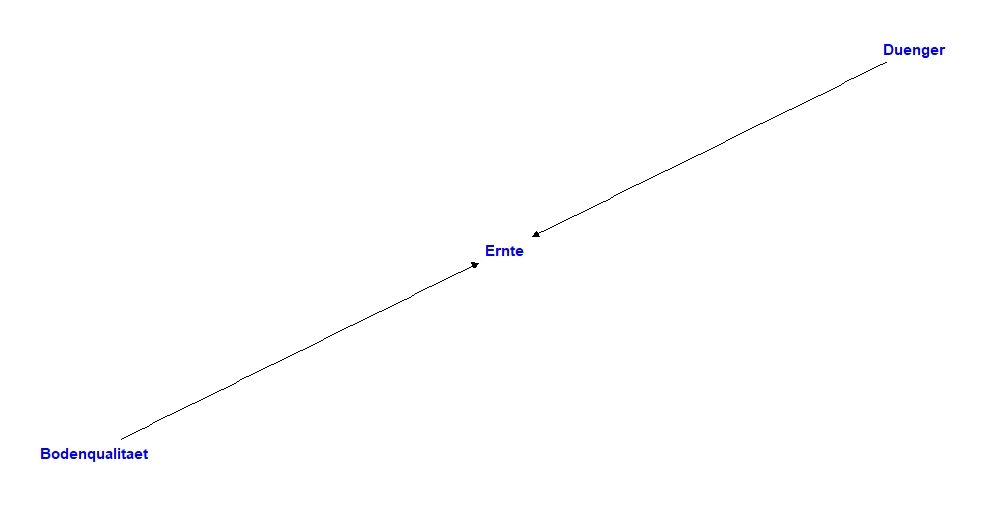
\includegraphics[width=0.8\linewidth]{Resources/DAGDuenger} 

}

\caption[Dünger]{Dünger}\label{fig:unnamed-chunk-1}
\end{figure}
\normalsize
\end{frame}

\begin{frame}{Was ist Ökonometrie und wofür brauchen wir sie?}
\protect\hypertarget{was-ist-uxf6konometrie-und-wofuxfcr-brauchen-wir-sie-3}{}
\begin{itemize}
\tightlist
\item
  In den meisten interessanteren Szenarien (wie die o.g.
  Bildungsrenditen) sind solche Experimente aus unterschiedlichen
  Gründen nicht möglich.
\item
  Stattdessen müssen wir typischerweise mit \hil{Beobachtungsdaten}
  arbeiten, die bereits bestehen werden und
  \alert{nicht in einem Experiment gesammelt wurden}.
\item
  Dann müssen wir statistisch alle anderen wichtigen Faktoren konstant
  halten.

  \begin{itemize}
  \tightlist
  \item
    Beispielsweise werden fähigere Personen mehr verdienen, sich aber
    auch \textit{entscheiden} mehr zu lernen.
  \item
    Höhergebildete haben zudem im Allgemeinen weniger
    Arbeitsmarkterfahrung, welche ebenfalls das Einkommen beeinflusst.
  \end{itemize}
\item
  Die Arbeitsmarkterfahrung ist recht \alert{leicht zu beobachten},
  wohingegen \glqq Fähigkeit\grqq{} \alert{schwer zu erfassen} ist.
\item
  Wir werden sehen, dass das Berücksichtigen von Faktoren wie dem
  Ersteren \alert{leicht} ist.
\item
  \alert{Komplizierter} wird es, wenn ein wichtiger Faktor nicht direkt
  beobachtet werden kann.
\end{itemize}
\end{frame}

\begin{frame}{Was ist Ökonometrie und wofür brauchen wir sie?}
\protect\hypertarget{was-ist-uxf6konometrie-und-wofuxfcr-brauchen-wir-sie-4}{}
\framesubtitle{DAG Lohnregression}

\begin{itemize}
\tightlist
\item
  Die \emph{angenommene} Problemstellung als DAG:
\end{itemize}

\footnotesize
\begin{figure}

{\centering 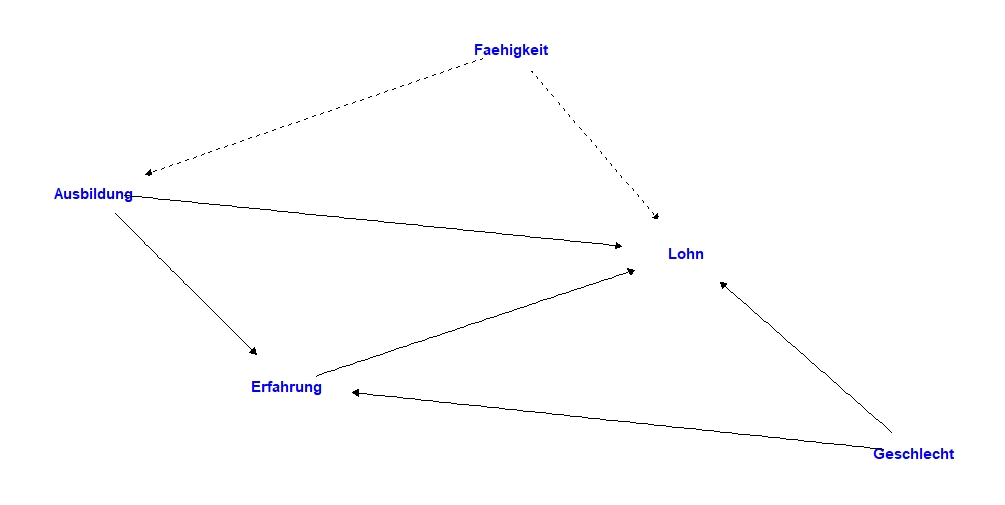
\includegraphics[width=0.8\linewidth]{Resources/DAGLoehne} 

}

\caption[Lohnregression]{Lohnregression}\label{fig:unnamed-chunk-2}
\end{figure}
\normalsize
\end{frame}

\begin{frame}{Gesundheitsökonomisches Beispiel}
\protect\hypertarget{gesundheitsuxf6konomisches-beispiel}{}
\begin{itemize}
\tightlist
\item
  Was ist der \alert{kausale Effekt} von Krankenversicherung (Health
  Insurance, HI) auf die Gesundheit (Health Index) in den USA?

  \begin{itemize}
  \tightlist
  \item
    Health Index ist Zahl von 5 (exzellent) bis 1 (schlecht).
  \end{itemize}
\item
  Betrachte Daten aus dem
  \alert{National Health Interview Survey (NHIS)} aus den USA.
\end{itemize}

\begin{table}[t!]
        \centering
        \begin{tabular}{lrr}
            \toprule
                 & Some HI & No HI  \\
\midrule
    &  \multicolumn{2}{c}{A. Gesundheit} \\
Health Index        &    4,01 & 3,70 \\
\midrule
    &  \multicolumn{2}{c}{B. Charakteristiken} \\
Nonwhite        &    0,16 & 0,17 \\
Age             &    43,98 & 41,26 \\
Education       &    14,31 & 11,56 \\
Family Size     &    3,50 & 3,98 \\
Employed        &    0,92 & 0,85 \\
Family Income   &    106.467 & 45.656 \\
Sample Size     &    8.114 & 1.281 \\
            \bottomrule
        \end{tabular}
\caption{Gesundheit und demografische Charakteristiken von Versicherten und Unversicherten im NHIS}
\label{tab:NHIS}
\end{table}
\end{frame}

\begin{frame}{Gesundheitsökonomisches Beispiel}
\protect\hypertarget{gesundheitsuxf6konomisches-beispiel-1}{}
\begin{itemize}
\tightlist
\item
  Oft: \alert{Unterschied in durchschnittlichem Health Index}
  (\(=4,01-3,70=0,31\)) wird (fälschlicherweise) als kausaler Effekt der
  Versicherung interpretiert.
\item
  Aber: Ein direkter Vergleich der Gesundheit von Versicherten und
  Unversicherten vergleicht \alert{Äpfel mit Birnen} -- nicht Äpfel mit
  Äpfeln.
\item
  Grund: Es gibt viele \alert{systematische Unterschiede} beider
  Gruppen, die für unterschiedlichen Health Index verantwortlich sein
  könnten:

  \begin{itemize}
  \tightlist
  \item
    Höhere Bildung (\(14,31>11,56\)) könnte gesundheitsförderlichen
    Lebensstil begünstigen.
  \item
    Höheres Einkommen (\(106.467>45.656\)) kann für gesunderes Essen
    ausgegeben werden.
  \end{itemize}
\item
  Mit anderen Worten: \emph{ceteris} ist \alert{nicht} \emph{paribus}
  hier!
\end{itemize}
\end{frame}

\begin{frame}{Gesundheitsökonomisches Beispiel}
\protect\hypertarget{gesundheitsuxf6konomisches-beispiel-2}{}
\begin{itemize}
\tightlist
\item
  Um die Problematik noch genauer zu verstehen, bezeichne mit \(Y\) den
  \alert{Health Index} einer Person und den \alert{Versicherungsstatus}
  mit \[
  D=\begin{cases} 1,& \text{Person ist versichert},\\
  0, &\text{sonst}.
  \end{cases}
  \]
\item
  Wir bezeichnen mit \(Y(1)\) (\(Y(0)\)) den Gesundheitszustand, wenn
  die Person versichert (nicht versichert) ist.

  \begin{itemize}
  \tightlist
  \item
    Natürlich beobachten wir die Welt nur in \alert{einem Zustand}, also
    \emph{entweder} \(Y(1)\) \emph{oder} \(Y(0)\).
  \end{itemize}
\item
  Damit ist \(Y(1)-Y(0)\) der \alert{individuelle kausale Effekt} von
  \(D\) auf \(Y\).
\end{itemize}

\xmpl

\begin{itemize}
  
  \item Betrachte 2 (hypothethische) Studierende am MIT in Boston.
  \item Gesunde \alert{Maria} und kränkelnder \alert{Khuzdar} mit $Y_{Maria}(1)=Y_{Maria}(0)=5$ und $Y_{Khuzdar}(1)=4$ und $Y_{Khuzdar}(0)=3$, so dass individuelle kausale Effekte
\begin{align*}
  Y_{Maria}(1)-Y_{Maria}(0)&=0,\\
  Y_{Khuzdar}(1)-Y_{Khuzdar}(0)&=1
\end{align*}
  
\end{itemize}

\endxmpl
\end{frame}

\begin{frame}{Gesundheitsökonomisches Beispiel}
\protect\hypertarget{gesundheitsuxf6konomisches-beispiel-3}{}
\xmpl[*]

\begin{table}[t!]
        \centering
        \begin{tabular}{lrr}
            \toprule
                 & Khuzdar & Maria  \\
\midrule
Potentielles Ergebnis ohne Versicherung $Y(0)$&  3 & 5 \\
Potentielles Ergebnis mit Versicherung $Y(1)$ &  4 & 5 \\
Behandlung $D$                                &  1 & 0 \\
Health Index $Y$                              &  4 & 5 \\
Individueller kausaler Effekt $Y(1)-Y(0)$)    &  1 & 0 \\
            \bottomrule
        \end{tabular}
\caption{Ergebnisse und Behandlung für Khuzdar und Maria}
\label{tab:KM}
\end{table}

\begin{itemize}
  \item \alert{Direkter Vergleich} von Khuzdar und Maria verrät nichts über kausale Effekte:
  \begin{align*}
    Y_{Khuzdar} - Y_{Maria} &= Y_{Khuzdar}(1) - Y_{Maria}(0)\\
    &= \underbrace{Y_{Khuzdar}(1) - Y_{Khuzdar}(0)}_{\text{Individueller kausaler Effekt}} + \underbrace{\big\{Y_{Khuzdar}(0) - Y_{Maria}(0)\big\}}_{\text{Selektionsverzerrung}} \\
    & = 1 -2 = -1.
  \end{align*}
  \item Weil die kerngesunde Maria mit dem kränklichen Khuzdar \alert{nicht vergleichbar} ist ($Y_{Khuzdar}(0) - Y_{Maria}(0)\neq0$), können wir nichts über kausale Effekte lernen!
\end{itemize}

\endxmpl
\end{frame}

\begin{frame}{Gesundheitsökonomisches Beispiel}
\protect\hypertarget{gesundheitsuxf6konomisches-beispiel-4}{}
\begin{itemize}
\tightlist
\item
  Mittelt sich \hil{Selektionsverzerrung} möglicherweise weg, wenn wir
  die ganze Grundgesamtheit betrachten und uns dann für den
  \alert{durchschnittlichen kausalen Effekt} \(\E\big[Y(1)-Y(0)\big]\)
  interessieren?
\item
  \alert{Nein}, denn wenn wir der Einfachheit halber
  \alert{konstante kausale Effekte} für alle unterstellen, also
  \begin{equation}\label{eq:const kap}
  \kappa = Y(1)-Y(0),
  \end{equation} dann ist ein Mittelwertvergleich (wie in
  Tabelle~\ref{tab:NHIS}) auch hier irreführend: \begin{multline*}
  \underbrace{\E[Y(1)\mid D=1] - \E[Y(0)\mid D=0]}_{\text{Differenz in Gruppenmittelwerten}} \\
  \overset{\eqref{eq:const kap}}{=} \underbrace{\kappa}_{\text{kausaler Effekt}} + \underbrace{\big\{\E[Y(0)\mid D=1] - \E[Y(0)\mid D=0]\big\}}_{\text{Selektionsverzerrung}}.
  \end{multline*}
\item
  Im Selektionsverzerrungs-Term fängt \(Y(0)\) alle
  gesundheitsrelevanten Faktoren ein \alert{außer} der Versicherung
  (z.B.~Einkommen und Bildung in Tabelle~\ref{tab:NHIS}).
\end{itemize}
\end{frame}

\begin{frame}{Ziel der Veranstaltung}
\protect\hypertarget{ziel-der-veranstaltung}{}
\begin{itemize}
\tightlist
\item
  Sie werden \ldots{}

  \begin{itemize}
  \tightlist
  \item
    \ldots{} ein tieferes Verständnis für das (lineare)
    Regressionsmodell entwickeln,
  \item
    \ldots{} die Methodik, Schlussfolgerungen aus selbigem zu ziehen,
    verstehen.
  \end{itemize}
\item
  So

  \begin{itemize}
  \tightlist
  \item
    \ldots{} können Sie die Validität Ihnen präsentierter
    ökonometrischer Studien kompetent einschätzen
  \item
    \ldots{} und eigene empirische Studien durchführen.
  \end{itemize}
\item
  Endziel meist die Schätzung \hil{kausaler} Effekte aufgrund von
  \hil{beobachteten Querschnittsdaten}.
\end{itemize}
\end{frame}

\begin{frame}{Überblick}
\protect\hypertarget{uxfcberblick-2}{}
\begin{itemize}
\tightlist
\item
  Organisatorisches
\item
  Ziele der Veranstaltung
\item
  \textbf{Wiederholung Wahrscheinlichkeitstheorie}
\end{itemize}
\end{frame}

\begin{frame}{Wiederholung}
\protect\hypertarget{wiederholung}{}
\begin{itemize}
\tightlist
\item
  Wir wiederholen hier kurz Grundbegriffe für bedingte Verteilungen,
  insbesondere \alert{bedingte Erwartungswerte}.
\item
  Bedingte Erwartungswerte werden im Rest der Veranstaltung ein
  \alert{zentrales Objekt} sein.

  \begin{itemize}
  \tightlist
  \item
    Warum, sehen wir später\ldots{}
  \end{itemize}
\end{itemize}
\end{frame}

\begin{frame}{Zufallsvariable}
\protect\hypertarget{zufallsvariable}{}
\begin{itemize}
\tightlist
\item
  Eine \hil{Zufallsvariable (ZV)} ist ein numerischer Wert mit
  Zufallselement.

  \begin{itemize}
  \tightlist
  \item
    Beispiel: Lohn (\(wage\)), der --
    \alert{bevor Sie jemanden gefragt haben} -- zufällig ist.
  \end{itemize}
\item
  \hil{Diskrete} ZVen nehmen endlich viele Werte an.

  \begin{itemize}
  \tightlist
  \item
    Beispiel: Geschlecht (\(gender\in\{0,1\}\))
  \end{itemize}
\item
  \hil{Stetige} ZVen nehmen Werte auf einem Kontinuum an.

  \begin{itemize}
  \tightlist
  \item
    Beispiel: Lohn (\(0\leq wage <\infty\)).
  \end{itemize}
\item
  Egal ob diskret oder stetig, die \hil{Verteilung} einer ZV \(Y\) ist
  eindeutig festgelegt durch die \hil{Verteilungsfunktion} \[
  F(y)=\Pr\{Y\leq y\}.
  \]
\item
  Wenn \(F(\cdot)\) differenzierbar ist (nur bei \alert{stetigen} ZVen
  möglich), nennen wir die Ableitung \hil{Dichtefunktion} von \(Y\): \[
  f(y)=(\partial/\partial y) F(y).
  \]
\item
  Das Gegenstück für \alert{diskrete} ZVen sind die
  \hil{Punktwahrscheinlichkeiten} \(\Pr\{Y=y_i\}\).
\end{itemize}
\end{frame}

\begin{frame}{Zufallsvariable}
\protect\hypertarget{zufallsvariable-1}{}
\xmpl[Löhne aus dem US CPS]

\begin{itemize}
\tightlist
\item
  Betrachte 50.742 Löhne (\(wage\)) aus dem US
  \hil{Current Population Survey (CPS)}.
\item
  Wir zeigen (geschätzte) \alert{Dichtefunktion} \(f(\cdot)\) der
  logarithmierten Löhne (\(\log(wage)\)).
\end{itemize}

\endxmpl

\footnotesize
\begin{center}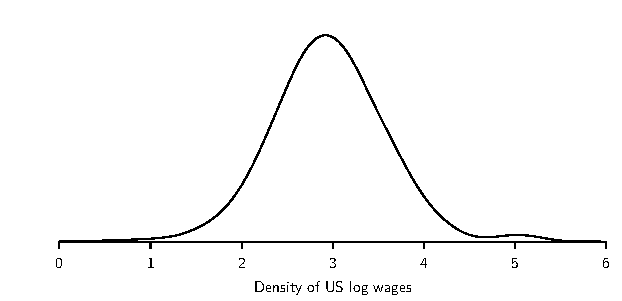
\includegraphics{Resources/Plots/wage-1} \end{center}
\normalsize
\end{frame}

\begin{frame}{Momente}
\protect\hypertarget{momente}{}
\begin{itemize}
\tightlist
\item
  Die Verteilung ist ein komplexes Objekt, aber \hil{Momente} bieten
  eine informative Zusammenfassung.
\item
  Der \hil{Erwartungswert} \(\E[Y]\) ist das \alert{zentrale Lagemaß}.

  \begin{itemize}
  \tightlist
  \item
    \(\E[Y]=\sum_{i=1}^{\infty}y_i\Pr\{Y=y_i\}\) für \alert{diskrete}
    \(Y\).
  \item
    \(\E[Y]=\int_{-\infty}^{\infty}y f(y) \mathrm{d} y\) für
    \alert{stetige} \(Y\).
  \end{itemize}
\item
  Man kann zeigen, dass sich der Erwartungswert der
  \alert{transformierten Variablen} \(g(Y)\) berechnet zu:

  \begin{itemize}
  \tightlist
  \item
    \(\E\big[g(Y)\big]=\sum_{i=1}^{\infty}g(y_i)\Pr\{Y=y_i\}\) für
    \alert{diskrete} \(Y\).
  \item
    \(\E\big[g(Y)\big]=\int_{-\infty}^{\infty}g(y) f(y) \mathrm{d} y\)
    für \alert{stetige} \(Y\).
  \end{itemize}
\item
  Die \hil{Varianz} \(\Var(Y)=\E(Y-\E[Y])^2\) ist das
  \alert{zentrale Streuungsmaß}.
\item
  Auch gerne benutzt wird die \hil{Standardabweichung}
  \(\sd(Y)=\sqrt{\Var(Y)}\).
\end{itemize}
\end{frame}

\begin{frame}{Momente}
\protect\hypertarget{momente-1}{}
\framesubtitle{Rechenregeln}

\thmn\label{eq:mom} Seien \(X\) und \(Y\) zwei Zufallsvariablen und
\(a,b\in\mathbb{R}\). Dann gelten:

\begin{itemize}
\tightlist
\item
  \(\E[X+Y]=\E[X]+\E[Y]\).
\item
  \(\E[aX+b]=a\E[X]+b\) \qquad~(``Linearität des Erwartungswertes'').
\item
  \(\Var(aX+b)=a^2\Var(X)\).
\item
  \(\Var(X)=\E[X^2]-\big(\E[X]\big)^2\) \qquad (``Verschiebungssatz'').
\item
  Sind \(X\) und \(Y\) unabhängig, so gilt
  \(\Var(X+Y)=\Var(X)+\Var(Y)\).
\end{itemize}

\endthmn
\end{frame}

\begin{frame}{Gemeinsame Verteilung}
\protect\hypertarget{gemeinsame-verteilung}{}
\begin{itemize}
\tightlist
\item
  Oft ist die \alert{Beziehung} zwischen zwei (oder mehreren) ZVen \(X\)
  und \(Y\) von Interesse.
\item
  Dafür führen wir den Begriff der \hil{gemeinsamen Verteilungsfunktion}
  ein: \[
  F(x,y) = \Pr\{X\leq x,\ Y\leq y\},\qquad x,y\in\mathbb{R}.
  \]
\item
  Anschaulicher ist oft die \hil{gemeinsame Dichtefunktion} \[
  f(x,y)=\frac{\partial^2 F(x,y)}{\partial x\partial y}
  \] oder, im diskreten Fall, die
  \hil{gemeinsamen Punktwahrscheinlichkeiten} \(\Pr\{X=x_j, Y=y_i\}\).
\end{itemize}
\end{frame}

\begin{frame}{Bedingte Verteilung}
\protect\hypertarget{bedingte-verteilung}{}
\begin{itemize}
\tightlist
\item
  Die \hil{bedingte Verteilung} ist oft eine anschauliche
  Zusammenfassung der gemeinsamen Verteilung.
\item
  Die bedingte Verteilung von \(Y\) gegeben \(X=x\) (geschrieben
  \(Y\mid X=x\)) ist eindeutig festgelegt durch die
  \hil{bedingte Verteilungsfunktion} \begin{align*}
  \Pr\{Y\leq y\mid X=x\} :=\begin{cases} \frac{\Pr\{Y\leq y,\ X=X\}}{\Pr\{X=x\}}& \text{für diskretes }X,\\
     \frac{\partial F(x,y)/\partial x}{f_X(x)} &\text{für stetiges }X.
     \end{cases}
  \end{align*}
\item
  Die \hil{bedingte Dichte} ist (falls sie existiert) die Ableitung der
  bedingten Verteilungsfunktion \[
  f_{Y\mid X=x}(y) = \frac{\partial \Pr\{Y\leq y\mid X=x\}}{\partial y}=\frac{f(x,y)}{f_X(x)}.
  \]
\item
  Das Pondon ist die \hil{bedingte Wahrscheinlichkeit} \[
  \Pr\{Y=y\mid X=x\}=\frac{\Pr\{X=x,\ Y=y\}}{\Pr\{X=x\}}.
  \]
\item
  \alert{Beachte:} Bedingte Verteilungsfunktionen und bedingte Dichten
  sind ganz übliche \alert{Verteilungsfunktionen} und \alert{Dichten}.
\end{itemize}
\end{frame}

\begin{frame}{Bedingte Verteilung}
\protect\hypertarget{bedingte-verteilung-1}{}
\xmpl[Löhne aus dem US CPS]

\begin{itemize}
\tightlist
\item
  Betrachte für die US CPS Daten die (geschätzte)
  \alert{bedingte Dichte} von

  \begin{center}
  $\log(wage)\mid gender,\qquad gender\in\{male,\ female\}.$
  \end{center}
\end{itemize}

\endxmpl

\footnotesize
\begin{center}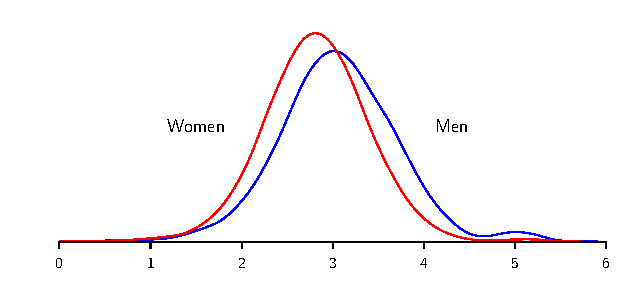
\includegraphics{Resources/Plots/wage2a-1} \end{center}
\normalsize
\end{frame}

\begin{frame}{Bedingte Momente}
\protect\hypertarget{bedingte-momente}{}
\begin{itemize}
\tightlist
\item
  Da bedingte Verteilungen auch wieder ganz übliche Dichten und
  Verteilungsfunktionen besitzen, können wir auch alle Momente
  \alert{analog} definieren.
\item
  Der \hil{bedingte Erwartungswert} \(\E[Y\mid X=x]\) ist \begin{align*}
  \E[Y\mid X=x] &= \sum_{i=1}^{\infty}y_i\Pr\{Y=y_i\mid X=x\}\quad\text{für diskrete Verteilung }Y\mid X=x,\\
  \E[Y\mid X=x] &= \int_{-\infty}^{\infty}y f_{Y\mid X=x}(y) \mathrm{d}y\quad\text{für stetige Verteilung }Y\mid X=x.
  \end{align*}
\item
  Oft bezeichnen wir auch \(\E[Y\mid X]\) als
  \alert{bedingten Erwartungswert:} Diesen interpretieren wir als eine
  von \(X\) abhängige Zufallsvariable, die für realisiertes \(X=x\) den
  Wert \(\E[Y\mid X=x]\) annimmt.
\end{itemize}
\end{frame}

\begin{frame}{Bedingte Momente}
\protect\hypertarget{bedingte-momente-1}{}
\begin{itemize}
\tightlist
\item
  Wenn \(Y\) transformiert ist, ergeben sich die bedingten
  Erwartungswerte (analog zum unbedingten Fall) zu: \begin{align}
  \E\big[g(Y)\mid X=x\big] &= \sum_{i=1}^{\infty}g(y_i)\Pr\{Y=y_i\mid X=x\}\quad\text{für diskrete Verteilung }Y\mid X=x,\notag\\
  \E\big[g(Y)\mid X=x\big] &= \int_{-\infty}^{\infty}g(y) f_{Y\mid X=x}(y) \mathrm{d}y\quad\text{für stetige Verteilung }Y\mid X=x.\label{eq:cE trafo}
  \end{align}
\item
  Die \hil{bedingte Varianz} ist definiert als \[
  \Var(Y\mid X=x) = \E\big[\{Y-\E(Y\mid X=x)\}^2\mid X=x\big].
  \]
\item
  Wie oben bezeichnen wir auch die Zufallsvariable \(\Var(Y\mid X)\) oft
  als \alert{bedingte Varianz:} Für realisiertes \(X=x\) nimmt sie den
  Wert \(\Var(Y\mid X=x)\) an.
\end{itemize}
\end{frame}

\begin{frame}{Bedingte Momente}
\protect\hypertarget{bedingte-momente-2}{}
\xmpl[Löhne aus dem US CPS]

\begin{itemize}
\tightlist
\item
  Männer verdienen im Schnitt mehr als Frauen, denn für den
  \alert{bedingten Erwartungswert} gilt: \[
  \E\big[\log(wage)\mid gender\big] = \begin{cases}
    \E\big[\log(wage)\mid female\big]=2.81,& gender = female,\\
    \E\big[\log(wage)\mid male\big]=3.05,& gender = male.
  \end{cases}
  \]
\item
  Die Lohnverteilung der Männer ist aber variabler, denn für die
  \alert{bedingte Varianz} gilt: \[
  \Var\big(\log(wage)\mid gender\big) = \begin{cases}
    \Var\big(\log(wage)\mid female\big)=0.37,& gender = female,\\
    \Var\big(\log(wage)\mid male\big)=0.50,  & gender = male.
  \end{cases}
  \]
\end{itemize}

\endxmpl
\end{frame}

\begin{frame}{Bedingte Momente}
\protect\hypertarget{bedingte-momente-3}{}
\footnotesize
\begin{center}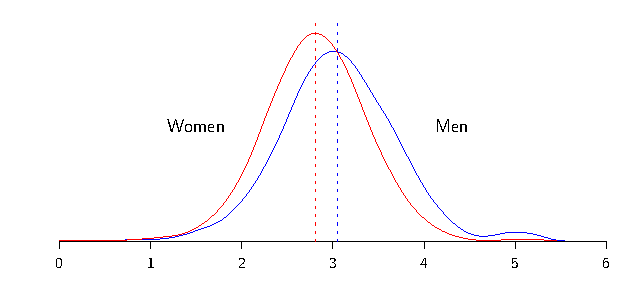
\includegraphics{Resources/Plots/wage3-1} \end{center}
\normalsize
\end{frame}

\begin{frame}{Bedingte Momente}
\protect\hypertarget{bedingte-momente-4}{}
\xmpl[Löhne aus dem US CPS]

\begin{itemize}
\tightlist
\item
  Der bedingte Erwartungswert lässt sich auch für \alert{stetige} \(X\)
  illustrieren.
\item
  Wir betrachten die Erwartungswertfunktion \(x\mapsto\E[Y\mid X=x]\)
  konkret für: \[
  \E\big[\log(wage)\mid experience \big],
  \] wobei \alert{$experience = age - education - 6$} die
  Arbeitsmarkterfahrung (gemessen in Jahren) approximiert.
\item
  Erinnern Sie sich für die folgende Grafik daran, dass für
  \alert{stetige $(X,Y)$} mit gemeinsamer Dichte \(f(x,y)\) gilt \[
  f_{Y\mid X=x}(y)=\frac{f(x,y)}{f_X(x)}.
  \]
\item
  Das heißt die bedingte Dichte \(y\mapsto f_{Y\mid X=x}(y)\) ist ein
  \alert{Schnitt} durch die gemeinsame Dichte \(f(x,y)\) für fixes
  \(x\), geeignet normalisiert (mit \(f_X(x)\), s.d.~sie wieder zu 1
  integriert), so dass sie selber wieder eine Dichte ist.
\end{itemize}

\endxmpl
\end{frame}

\begin{frame}{Bedingte Momente}
\protect\hypertarget{bedingte-momente-5}{}
\footnotesize
\begin{center}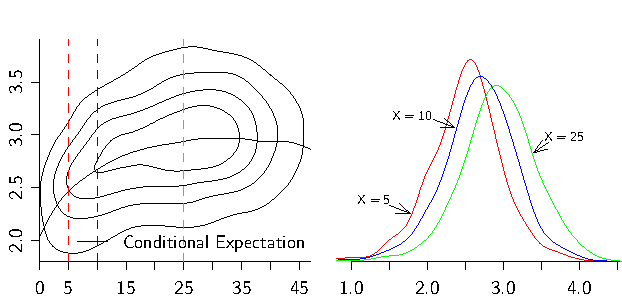
\includegraphics{Resources/Plots/wage4-1} \end{center}
\normalsize
\begin{center}
Labor market experience (years)\,\,\qquad\qquad Log dollars per hour
\end{center}

\begin{center}
\qquad (a) Gemeinsame Dichte von \qquad\qquad (b) Bedingte Dichte von log 
\end{center}
\vspace{-0.5cm}
\begin{center}
\qquad\,\, log wage und experience \quad\qquad\qquad wage gegeben experience
\end{center}
\end{frame}

\begin{frame}{Bedingte Momente}
\protect\hypertarget{bedingte-momente-6}{}
\framesubtitle{Rechenregeln}

\begin{itemize}
\tightlist
\item
  Die üblichen Rechenregeln für \emph{un}bedingte Erwartungen aus
  Theorem \ref{eq:mom} gelten auch für bedingte Erwartungen:
\end{itemize}

\thmn\label{thm:bed mom} Seien \(X\), \(Y\) und \(Z\) drei
Zufallsvariablen und \(a,b\in\mathbb{R}\). Dann gelten:

\begin{itemize}
\tightlist
\item
  \(\E[X+Y\mid Z]=\E[X\mid Z]+\E[Y\mid Z]\).
\item
  \(\E[aX+b\mid Z]=a\E[X\mid Z]+b\) \qquad~(``Linearität des bedingten
  Erwartungswertes'').
\item
  \(\Var(aX+b\mid Z)=a^2\Var(X\mid Z)\).
\item
  \(\Var(X\mid Z)=\E[X^2\mid Z]-(\E[X\mid Z])^2\)
  \qquad (``Verschiebungssatz'').
\item
  Sind \(X\) und \(Y\) unabhängig, so gilt
  \begin{equation}\label{eq:bE indep}
  \E[Y\mid X] = \E[Y].
  \end{equation}
\end{itemize}

\endthmn
\end{frame}

\begin{frame}{Eigenschaften der bedingten Erwartung}
\protect\hypertarget{eigenschaften-der-bedingten-erwartung}{}
\thmn[\hil{Gesetz vom iterierten Erwartungswert (GIE)}]Wenn
\(\E|Y|<\infty\), dann gilt für jede ZV \(X\)
\begin{equation}\label{eq:GIE}
  \E\big[\E[Y\mid X]\big]=\E[Y].
\end{equation} \endthmn

\xmpl[Löhne]

\begin{itemize}
\tightlist
\item
  Nach dem GIE gilt \begin{align*}
  \E\big[\log(wage)\big] & = \E\big(\E[\log(wage)\mid gender]\big)\\
  &= \E\big[\log(wage)\mid gender=male\big]\Pr\{gender = male\}+\\
  &\hspace{2cm} \E\big[\log(wage)\mid gender=female\big]\Pr\{gender = female\}.
  \end{align*}
\item
  D.h.~der Durchschnittslohn ist eine \alert{gewichtete Summe} der
  Durchschnittslöhne von Männern und Frauen -- das macht auch Sinn!
\end{itemize}

\endxmpl
\end{frame}

\begin{frame}{Eigenschaften der bedingten Erwartung}
\protect\hypertarget{eigenschaften-der-bedingten-erwartung-1}{}
\begin{itemize}
\tightlist
\item
  Das GIE gilt sogar \alert{allgemeiner:}
\end{itemize}

\thmn["Der Dümmere gewinnt"]Wenn \(\E|Y|<\infty\), dann gilt für ZVen
\(X_1\) und \(X_2\) \begin{equation}\label{eq:GIE advanced}
  \E\big[\E(Y\mid X_1,X_2)\mid X_1\big]=\E[Y\mid X_1]=\E\big[\E(Y\mid X_1)\mid X_1,X_2\big].
\end{equation} \endthmn

\begin{itemize}
\tightlist
\item
  Unter gewissen Bedingungen kann man aus der bedingten Erwartung
  \alert{Faktoren herausziehen:}
\end{itemize}

\thmn

Wenn \(\E|Y|<\infty\), dann gilt jede ZV \(X\) und für beliebige
Funktionen \(h(\cdot)\) \begin{equation}\label{eq:pull out}
  \E\big[h(X)Y\mid X\big]=h(X)\E[Y\mid X].
\end{equation} \endthmn
\end{frame}

\hypertarget{regression-projektion-und-kausalituxe4t}{%
\section{Regression, Projektion und
Kausalität}\label{regression-projektion-und-kausalituxe4t}}

\begin{frame}{}
\protect\hypertarget{section}{}
\centerline{\textbf{Regression, Projektion und Kausalität}}
\centerline{(Hansen, 2022, Kapitel 2)}
\end{frame}

\begin{frame}{Überblick}
\protect\hypertarget{uxfcberblick-3}{}
\begin{itemize}
\tightlist
\item
  \textbf{Bedingte Erwartung}
\item
  Lineare Projektion
\item
  Kausalität
\item
  Zusammenfassung
\end{itemize}
\end{frame}

\begin{frame}{Bedingte Erwartung und Prognose}
\protect\hypertarget{bedingte-erwartung-und-prognose}{}
\begin{itemize}
\tightlist
\item
  Wir wollen das \hil{bedingte Erwartungswertmodell} einführen.
\item
  Dazu betrachten wir folgendes \alert{Problem:} Gegeben \(X\), was ist
  die optimale Funktion \(g(X)\), um \(Y\) vorherzusagen?

  \begin{itemize}
  \tightlist
  \item
    Dies ist eine klassische Aufgabe aus dem \hil{Supervised Learning}
    als Teilbereich des \hil{Machine Learning}.
  \end{itemize}
\end{itemize}

\bigskip

\begin{itemize}
\tightlist
\item
  \alert{Achtung:} Für den Rest der Vorlesung schreiben wir Vektoren /
  Matrizen fett (z.B.~\(\mA\) anstatt \(A\) für eine Matrix) und Skalare
  normal (also \(y\) anstatt \(\vy\) für eine Zahl), \ldots
\item
  \ldots \alert{außer} bei unseren Prädiktoren / Regressoren \(X\) (und
  manchmal auch \(Z\)).
\item
  \alert{Zwei Gründe:}

  \begin{enumerate}
  \tightlist
  \item
    Einzelner Regressor, wie \(X=1\) auch möglich (aber sehr selten).
  \item
    \(\mX\) brauchen wir als Schreibweise, wenn wir Matrixnotation für
    das lineare Regressionsmodell einführen; siehe
    \eqref{eq:Matrixnotation}.
  \end{enumerate}
\end{itemize}
\end{frame}

\begin{frame}{Optimale Vorhersage}
\protect\hypertarget{optimale-vorhersage}{}
\begin{itemize}
\tightlist
\item
  Welches \(g\) optimal ist, hängt von unserer \hil{Verlustfunktion}
  \(L\) ab.
\item
  Wir benutzen den \hil{quadratischen Fehler} \[
  L\big(Y, g(X)\big) = \big(Y - g(X)\big)^2.
  \]

  \begin{itemize}
  \tightlist
  \item
    Viele andere denkbar, z.B.~\hil{absoluter Fehler}
    \(L\big(Y, g(X)\big) = |Y - g(X)|\), \ldots{}
  \item
    \ldots{} aber quadratischer Fehler liefert oft geschlossene Lösungen
    (z.B.~für Schätzer).
  \end{itemize}
\item
  Der \emph{zufällige} Verlust soll im Durchschnitt klein sein.
\item
  Also sollte gute Vorhersage geringes \hil{Risiko} \[
  R\big(Y, g(X)\big)=\E\big[L\big(Y, g(X)\big)\big]
  \] liefern.
\item
  Hier: Risiko ist der \hil{mittlere quadratische Fehler (MQF)} \[
  R\big(Y, g(X)\big)=\E\big[\big(Y - g(X)\big)^2\big].
  \]
\end{itemize}
\end{frame}

\begin{frame}{Optimales \(g\)?}
\protect\hypertarget{optimales-g}{}
\begin{itemize}
\tightlist
\item
  \alert{Aufgabe} somit: Finde \(g\), welches MQF minimiert.\medskip
\end{itemize}

\thmn[Hansen (2022, Theorem 2.7)]\label{thm:Opt Cond Exp} Wenn
\(\E[Y^2]<\infty\), dann wird der MQF minimiert durch die
\hil{bedingte Erwartungswertfunktion} \[
  m(X)=\E[Y\mid X].
\] Wir sagen \(m(X)\) ist der \hil{beste Prädiktor (BP)} von \(Y\)
gegeben \(X\). \endthmn

\medskip

\begin{itemize}
\tightlist
\item
  Das führt uns zum \alert{bedingten Erwartungswertmodell}
  \begin{equation}\label{eq:bE}
  Y= m(X)+[Y-m(X)] = m(X) + \epsilon
  \end{equation} mit \(\epsilon=Y-m(X)\) dem \hil{Regressionsfehler}.

  \begin{itemize}
  \tightlist
  \item
    Dieses Modell existiert \emph{für alle} \((Y,X)\) (sofern
    \(\E[Y\mid X]\) existiert).
  \end{itemize}
\item
  Die \alert{definierende} Eigenschaft des Regressionsfehlers ist, dass
  \begin{equation}\label{eq:error lbE}
  \E[\epsilon\mid X]\overset{\eqref{eq:bE}}{=}\E[Y-m(X)\mid X]\overset{\eqref{eq:pull out}}{=}\E[Y\mid X]-m(X)=0.
  \end{equation}
\end{itemize}
\end{frame}

\begin{frame}{Eigenschaften des Regressionsfehlers}
\protect\hypertarget{eigenschaften-des-regressionsfehlers}{}
\begin{itemize}
\tightlist
\item
  Aus der obigen definierenden Eigenschaft folgen:
\item
  Der Regressionsfehler hat \alert{Erwartungswert Null}, da
  \begin{equation}\label{eq:mean zero}
  \E[\epsilon] \overset{\eqref{eq:GIE}}{=} \E\big[\E(\epsilon\mid X)\big]\overset{\eqref{eq:error lbE}}{=}\E[0]=0.
  \end{equation}
\item
  Der Regressionsfehler ist \alert{unkorreliert} mit jeder Funktion von
  \(X\), da \begin{equation}\label{eq:uncorr}
  \E[h(X)\epsilon] \overset{\eqref{eq:GIE}}{=} \E\big[\E(h(X)\epsilon\mid X)\big]\overset{\eqref{eq:pull out}}{=} \E\big[h(X)\E(\epsilon\mid X)\big]\overset{\eqref{eq:error lbE}}{=}0
  \end{equation} und somit \[
   \Cov(h(X), \epsilon)=\underbrace{\E\big[h(X)\epsilon\big]}_{\overset{\eqref{eq:uncorr}}{=}0} - \E\big[h(X)\big]\underbrace{\E\big[\epsilon\big]}_{\overset{\eqref{eq:mean zero}}{=}0}=0.
  \]
\end{itemize}
\end{frame}

\begin{frame}{}
\protect\hypertarget{section-1}{}
\begin{proof}[Beweis von Theorem \ref{thm:Opt Cond Exp}]
Für beliebiges $g$ ergibt sich der MQF zu
\begin{align*}
  \E&\Big[\big\{Y-g(X)\big\}^2\Big] \\
  &= \E\Big[\big\{Y-m(X) + m(X) - g(X)\big\}^2\Big]\\
  &= \E\Big[\big\{Y-m(X)\big\}^2\Big] + 2\E\Big[\big\{Y-m(X)\big\}\big\{m(X)-g(X)\big\}\Big] +\E\Big[\big\{m(X)-g(X)\big\}^2\Big]\\ 
  &= \E\Big[\big\{Y-m(X)\big\}^2\Big] +\E\Big[\big\{m(X)-g(X)\big\}^2\Big]\\
  &\geq \E\Big[\big\{Y-m(X)\big\}^2\Big],
\end{align*}
wobei wir ausgenutzt haben, dass
\[
  2\E\Big[\big\{Y-m(X)\big\}\big\{m(X)-g(X)\big\}\Big]\overset{\text{Def. }\epsilon}{=}2\E\Big[\epsilon\big\{m(X)-g(X)\big\}\Big]\overset{\eqref{eq:uncorr}}{=}0.
\]
\end{proof}
\end{frame}

\begin{frame}{Bedingtes Erwartungswertmodell}
\protect\hypertarget{bedingtes-erwartungswertmodell}{}
\begin{itemize}
\tightlist
\item
  Ein (prominenter) \alert{Spezialfall} des bedingten
  Erwartungswertmodells ergibt sich, wenn \[
  m(x)=\E[Y\mid X=x]=x^\prime\vbeta=x_1\beta_1 + \ldots + x_k\beta_k
  \] für einen Parametervektor
  \(\vbeta=(\beta_1,\ldots,\beta_k)^\prime\).\bigskip
\end{itemize}

\defn[Lineares bedingtes Erwartungswertmodell]Das Modell \begin{align}
  Y &= X^\prime\vbeta + \epsilon,\label{eq:Regressionsfehler}\\
  \E[\epsilon\mid X] &=0,\notag
\end{align} heißt \hil{lineares bedingtes Erwartungswertmodell}.
\enddefn
\end{frame}

\begin{frame}{Beispiel}
\protect\hypertarget{beispiel}{}
\framesubtitle{Linearität entsteht oft ganz  natürlich...}

\xmpl[Bivariate Normalverteilung]\label{ex:Biv Norm}

\begin{itemize}
\item Sei 
\[
  \begin{pmatrix}Y\\X \end{pmatrix}\sim N\Bigg(\begin{pmatrix}\mu_Y\\ \mu_X \end{pmatrix}, \begin{pmatrix}\sigma_Y^2 & \rho\sigma_Y\sigma_X\\ \rho\sigma_Y\sigma_X & \sigma_X^2 \end{pmatrix}\Bigg),
\]
wobei $\rho$ die Korrelation zwischen $X$ und $Y$ bezeichnet.
\item Dann gilt
\[
  \E[Y\mid X] = \mu_Y + \rho\frac{\sigma_Y}{\sigma_X}(X-\mu_X).
\]
\item Also ist der bedingte Erwartungswert eine \alert{lineare Funktion} in $x$.
\end{itemize}
\endxmpl
\end{frame}

\begin{frame}{Verschiedene Perspektiven}
\protect\hypertarget{verschiedene-perspektiven}{}
\begin{itemize}
\item
  Standard Ökonometrie Lehrbücher: Nehmen an, dass \[
  Y=m(X)+\epsilon,\qquad \E[\epsilon\mid X]=0,
  \] der wahre \hil{datengenerierende Prozess (DGP)} ist.
\item
  Hier: \alert{DGP egal}; suchen nur Funktion \(m(X)\), um \(Y\) so
  genau wie möglich vorherzusagen (gemessen in MQF).
\end{itemize}
\end{frame}

\begin{frame}{Überblick}
\protect\hypertarget{uxfcberblick-4}{}
\begin{itemize}
\tightlist
\item
  Bedingte Erwartung
\item
  \textbf{Lineare Projektion}
\item
  Kausalität
\item
  Zusammenfassung
\end{itemize}
\end{frame}

\begin{frame}{Lineare Projektion}
\protect\hypertarget{lineare-projektion}{}
\begin{itemize}
\tightlist
\item
  I.A.~ist der \alert{global} beste Prädiktor \(m(X)=\E[Y\mid X]\) eine
  \alert{komplexe Funktion von $X$}, die \emph{in praxi} unbekannt ist.
\item
  Deshalb machen wir unsere Vorhersageaufgabe nun \alert{einfacher}.
\item
  Minimiere den MQF nur unter allen \alert{linearen} Funktionen
  \(g(X)=X^\prime\vb\).
\item
  Die \alert{Lösung} ist der \hil{lineare Projektionskoeffizient} \[
  \vbeta=\argmin_{\vb\in\mathbb{R}^{k}}\E\big[(Y-X^\prime\vb)^2\big].
  \]
\item
  Um das Problem sauber zu lösen, brauchen wir einige \alert{Annahmen:}
\end{itemize}

\ass\label{ass:1}

\begin{enumerate}
  \item $\E[Y^2]<\infty$, 
  \item $\E[X_i^2]<\infty$ für alle $i$, wobei $X=(X_1,\ldots,X_k)^\prime$,
  \item $\E[XX^\prime]$ ist positiv definit (p.d.).
\end{enumerate}
\endass
\end{frame}

\begin{frame}{Lineare Projektionskoeffizienten}
\protect\hypertarget{lineare-projektionskoeffizienten}{}
\begin{itemize}
\tightlist
\item
  Unter Annahme \ref{ass:1} gilt für den
  \alert{linearen Projektionskoeffizienten}, dass
  \begin{equation}\label{eq:proj coeff}
  \vbeta=\big(\E[XX^\prime]\big)^{-1}\E[X Y].
  \end{equation}
\item
  \alert{Warum?} Der MQF ist \begin{align}
  \E\big[(Y-X^\prime\vb)^2\big] &= \E[Y^2] - 2\big(\E[X Y]\big)^\prime\vb + \vb^\prime\E[XX^\prime]\vb\label{eq:MQF calc}\\
  &=:a-2\va^\prime\vb+\vb^\prime\mA\vb\notag\\
  &=(a-\va^\prime\mA^{-1}\va) + (\vb-\mA^{-1}\va)^\prime\mA(\vb-\mA^{-1}\va)=:S(\vb).\notag
  \end{align}

  \begin{itemize}
  \tightlist
  \item
    Beachte: \(\mA^{-1}\) existiert, weil \(\E[XX^\prime]\) p.d. (siehe
    Prop.~\zref{S-prop:pd and det} und
    Def.~\zref{S-matrixproperties}.\zref{S-it:9.3})
  \end{itemize}
\item
  \alert{Erster Term} hängt nicht von \(\vb\) ab.
\item
  \alert{Zweiter Term} ist \(>0\), wenn \(\vb\neq\mA^{-1}\va\), und
  \(=0\), wenn \(\vb=\mA^{-1}\va\) (beides weil \(\mA\) p.d.)
\item
  Damit ist \(\vbeta=\mA^{-1}\va=\big(\E[XX^\prime]\big)^{-1}\E[X Y]\)
  sogar der \alert{eindeutige} Minimierer.
\end{itemize}
\end{frame}

\begin{frame}{BLP und Projektionsfehler}
\protect\hypertarget{blp-und-projektionsfehler}{}
\begin{itemize}
\tightlist
\item
  Mit obigem \(\vbeta\) ist der \hil{beste lineare Prädiktor (BLP)} von
  \(Y\) gegeben \(X\) \begin{equation}\label{eq:BLP eq}
  \mathcal{P}(Y\mid X)=X^\prime\vbeta=X^\prime \big(\E[XX^\prime]\big)^{-1}\E[X Y].
  \end{equation}
\item
  Der \hil{Projektionsfehler} ist \[
  e=Y-X^\prime\vbeta.
  \]

  \begin{itemize}
  \tightlist
  \item
    Dieser ist gleich dem Regressionsfehler \(\epsilon\) aus
    \eqref{eq:Regressionsfehler} \alert{dann und nur dann, wenn} die
    bedingte Erwartung linear in \(X\) ist.
  \end{itemize}
\item
  Die \alert{definierende} Eigenschaft des Projektionsfehlers ist, dass
  \begin{eqnarray*}
  \E[X e] &=& \E\big[X(Y-X^\prime\vbeta)\big]\\
            &\overset{\eqref{eq:proj coeff}}{=}& \E[X Y] - \E[XX^\prime]\big(\E[XX^\prime]\big)^{-1}\E[X Y]=\vzero.
  \end{eqnarray*}
\item
  Wenn \(X\) eine Konstante enthält, folgt somit \(\E[e]=0\) und daher
  \(\Cov(X_i,e)=\E[X_i e]=0\), d.h.~der Projektionsfehler und die
  Regressoren sind \alert{unkorreliert}.
\end{itemize}
\end{frame}

\begin{frame}{Lineares Projektionsmodell}
\protect\hypertarget{lineares-projektionsmodell}{}
\defn[Lineares Projektionsmodell]Das Modell \begin{align*}
  Y &= X^\prime\vbeta + e,\\
  \E[X e ] &=\vzero,\\
  \vbeta&=\big(\E[XX^\prime]\big)^{-1}\E[X Y],
\end{align*} heißt \hil{lineares Projektionsmodell}. \enddefn

\begin{itemize}
\tightlist
\item
  Das lineare Projektionsmodell \alert{existiert sehr allgemein},
  nämlich unter Annahme \ref{ass:1} -- insbesondere keine Annahme über
  linearen bedingten EW (wie im linearen bedingten
  Erwartungswertmodell).
\item
  Aber \alert{Obacht:} I.A. ist \(X^\prime\vbeta\) ``nur'' der BLP und

  \begin{itemize}
  \tightlist
  \item
    \emph{nicht} der bedingte Erwartungswert (also der global beste
    Prädiktor),
  \item
    noch beschreibt es einen strukturellen (kausalen) ökonomischen
    Zusammenhang.
  \end{itemize}
\end{itemize}
\end{frame}

\begin{frame}{Beispiel}
\protect\hypertarget{beispiel-1}{}
\xmpl[Vergleich: Projektion \& bedingter EW]

\begin{itemize}
\item Betrachte $Y=X+X^2$ mit $X\sim N(0,1)$.
\item Dann gilt 
\[
  m(X)=X+X^2
\]
und somit $\epsilon=0$ im \alert{linearen bedingten Erwartungswertmodell}.
\item Im \alert{linearen Projektionsmodell} $Y=\beta_0+\beta_1X + e$ gilt
\[
  \mathcal{P}(Y\mid X)=X+1,
\]
da $X$ und $X^2$ wegen der Normalverteilungsannahme unkorreliert sind.
\begin{itemize}
  \item Die lineare Projektion $\mathcal{P}(Y\mid X)=X+1$ ist also etwas gänzlich anderes als der lineare bedingte Erwartungswert $m(X)=X+X^2$!
\end{itemize}
\item Daher: $e=X^2-1$ ist der Projektionsfehler.
\end{itemize}
\endxmpl
\end{frame}

\begin{frame}{Beispiel}
\protect\hypertarget{beispiel-2}{}
\footnotesize
\begin{center}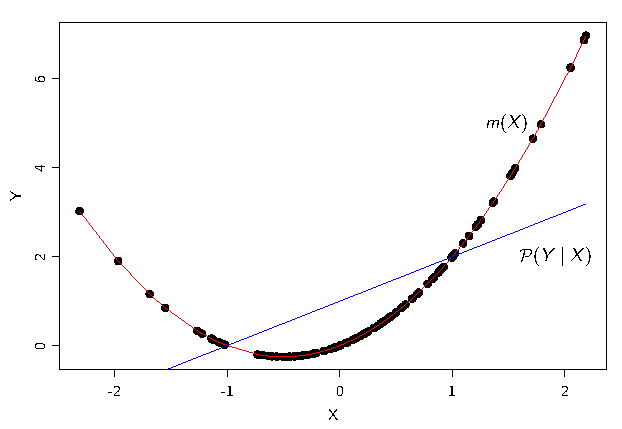
\includegraphics{Resources/Plots/ProjExp-1} \end{center}
\normalsize
\end{frame}

\begin{frame}{Weitere Interpretation des BLP}
\protect\hypertarget{weitere-interpretation-des-blp}{}
\begin{itemize}
\tightlist
\item
  I.A. ist der bedingte Erwartungswert \(\E[Y\mid X]\)
  \alert{NICHT linear}.
\item
  Was ist aber die \alert{beste lineare Approximation} von
  \(\E[Y\mid X]\)?
\item
  \alert{Antwort:} \(X^\prime\vbeta\) ist nicht nur der BLP von \(Y\),
  sondern auch der BLP von \(\E[Y\mid X]\)!
\item
  \alert{Begründung:} Der MQF ist (ähnlich wie in \eqref{eq:MQF calc})
  \begin{equation*}
  \E\big[(m(X)-X^\prime\vb)^2\big] = \E[m^2(X)] - 2\big(\E[X m(X)]\big)^\prime\vb + \vb^\prime\E[XX^\prime]\vb.
  \end{equation*}
\item
  Daher mit dem GIE: \begin{eqnarray*}
  \vbeta &\overset{\text{w.o.}}{=}&\big(\E[XX^\prime]\big)^{-1}\E[X m(X)]\\
  &\overset{\eqref{eq:bE}}{=}& \big(\E[XX^\prime]\big)^{-1}\E\big[X (Y-\epsilon)\big]\\
  &=& \big(\E[XX^\prime]\big)^{-1}\big(\E[XY] -  \E[X\epsilon]\big)\\
  &\overset{\eqref{eq:uncorr}}{=}& \big(\E[XX^\prime]\big)^{-1}\E[X Y].
  \end{eqnarray*}
\item
  Also: \(X^\prime\vbeta\) ist \alert{sowohl} der BLP von \(Y\)
  \alert{als auch} der von \(m(X)\)!
\end{itemize}
\end{frame}

\begin{frame}{Überblick}
\protect\hypertarget{uxfcberblick-5}{}
\begin{itemize}
\tightlist
\item
  Bedingte Erwartung
\item
  Lineare Projektion
\item
  \textbf{Kausalität}
\item
  Zusammenfassung
\end{itemize}
\end{frame}

\begin{frame}{Potential Outcomes Framework}
\protect\hypertarget{potential-outcomes-framework}{}
\xmpl[Lohnregression]

\begin{itemize}
  \item \alert{Endziel} häufig: Was ist der kausale Effekt?
  \item Z.B.: Was ist der kausale Effekt des \alert{Studiums} auf den \alert{Lohn}?
  \item Wir vergleichen Ihren Lohn in einer Welt, in der Sie studiert haben (bezeichnet $Y(1)$) 
  \item ... mit dem Lohn in einer Welt, in der Sie nicht studiert haben (bezeichnet $Y(0)$).
  \item Die Differenz $Y(1)-Y(0)$ ist dann der individuelle kausale Effekt des Studiums.
\end{itemize}
\endxmpl

\begin{itemize}
\tightlist
\item
  \alert{Probleme:}

  \begin{enumerate}
  \tightlist
  \item
    Kausaler Effekt ist individuenspezifisch.
  \item
    Kausaler Effekt nicht beobachtbar.
  \end{enumerate}
\item
  Also führen wir nun das \hil{Potential Outcomes Framework} von Rubin
  (1974) ein\ldots{}
\end{itemize}
\end{frame}

\begin{frame}{Potential Outcomes Framework}
\protect\hypertarget{potential-outcomes-framework-1}{}
\begin{itemize}
\tightlist
\item
  Im einfachsten Fall unterstellt das Potential Outcomes Framework für
  den \hil{Outcome} \begin{equation}\label{eq:R easy}
  Y=h(D,u),
  \end{equation} wobei \(D\) das binäre \hil{Treatment} ist, \(u\) ein
  individuenspezifischer Zufallsfaktor (ersetzt vorherige \(e\) und
  \(\epsilon\)), und \(h\) eine Funktion.
\item
  \(Y(1)=h(1,u)\) und \(Y(0)=h(0,u)\) sind die \hil{Potential Outcomes},
  die zum Treatment (\(D=1\)) bzw. Nicht-Treatment (\(D=0\)) gehören.
\end{itemize}

\defn[Kausaler Effekt]Im Modell \eqref{eq:R easy} ist der
\hil{individuelle kausale Effekt} von \(D\) auf \(Y\) \[
  Y(1)-Y(0),
\] also die Veränderung in \(Y\) aufgrund des Treatments während \(u\)
konstant bleibt.\medskip

Auf Englisch bezeichnen wir diesen als
\hil{individual treatment effect}. \enddefn
\end{frame}

\begin{frame}{Potential Outcomes Framework}
\protect\hypertarget{potential-outcomes-framework-2}{}
\begin{itemize}
\tightlist
\item
  Mit Heraklit (``Man kann nicht zweimal in denselben Fluss steigen.'')
  beobachten wir aber immer nur \alert{einen} Zustand der Welt (entweder
  \(D=1\) oder \(D=0\)).
\item
  Also können wir \alert{nichts} über den kausalen Effekt \(Y(1)-Y(0)\)
  lernen -- m.a.W.~er ist nicht \hil{operational}, d.h.~er kann nicht
  aus der Population heraus geschätzt werden.
\item
  Wenn wir mehrere Leute beobachten, besteht aber Hoffnung etwas über
  den \alert{durchschnittlichen} kausalen Effekt zu lernen:\bigskip
\end{itemize}

\defn[ATE]Im Modell \eqref{eq:R easy} ist der
\hil{durchschnittliche kausale Effekt} von \(D\) auf \(Y\) \[
  ATE=\E\big[Y(1)-Y(0)\big].
\] Auf Englisch bezeichnen wir diesen als
\hil{average treatment effect (ATE)}. \enddefn

\begin{itemize}
\tightlist
\item
  Während es hoffnungslos ist \(Y(1)-Y(0)\) zu schätzen, können wir über
  den \(ATE\) \alert{unter bestimmten Voraussetzungen} etwas aus Daten
  lernen\ldots{}
\end{itemize}
\end{frame}

\begin{frame}{Schätzung des ATE}
\protect\hypertarget{schuxe4tzung-des-ate}{}
\begin{itemize}
\tightlist
\item
  Unter folgender Annahme können wir den ATE schätzen:
\end{itemize}

\ass[\hil{Unabhängigkeitsannahme (UA)}]Das Treatment \(D\) ist
statistisch \alert{unabhängig} von \(u\). \endass

\begin{itemize}
\tightlist
\item
  Denn dann gilt: \begin{align*}
  \E\big[Y(1)\mid D=1\big] &\overset{\eqref{eq:R easy}}{=} \E\big[h(1,u)\mid D=1\big]\overset{\eqref{eq:bE indep}}{=}\E\big[h(1,u)\big]\overset{\eqref{eq:R easy}}{=}\E\big[Y(1)\big],\\
  \E\big[Y(0)\mid D=0\big] &\overset{\eqref{eq:R easy}}{=} \E\big[h(0,u)\mid D=0\big]\overset{\eqref{eq:bE indep}}{=}\E\big[h(0,u)\big]\overset{\eqref{eq:R easy}}{=}\E\big[Y(0)\big].
  \end{align*}
\item
  Der ATE wird dann \alert{operational}, weil er als Differenz der
  erwarteten Outcomes der Behandelten und Unbehandelten berechnet werden
  kann: \[
  ATE=\E\big[Y(1)\mid D=1\big]-\E\big[Y(0)\mid D=0\big].
  \]
\item
  Daher \alert{ideal:} Lotterie, die Leute zufällig (also unabhängig von
  ihren unbeobachteten Faktoren in \(u\)) in \hil{Behandlungsgruppe}
  (\(D=1\)) und \hil{Kontrollgruppe} (\(D=0\)) zuteilt.
\end{itemize}
\end{frame}

\begin{frame}{Schätzung des ATE}
\protect\hypertarget{schuxe4tzung-des-ate-1}{}
\xmpl[Lohnregression]

\begin{itemize}
  \item<1-> Inspiriert durch obige Ausführungen \alert{behaupten} wir, dass der durchschnittliche kausale Effekt eines Studiums ($D$) auf den Lohn $Y$ geschätzt werden kann als Durchschnittsverdienst der Studierten minus dem der Nicht-Studierten:
  \[
    \frac{1}{\#\{i\colon D_i=1\}}\sum_{i\colon D_i=1}Y_i - \frac{1}{\#\{i\colon D_i=0\}}\sum_{i\colon D_i=0}Y_i.
  \]
  \item<1-> \alert{Frage:} Kann dies als durchschnittlicher kausaler Effekt (ATE) interpretiert werden?
  \item<1-> \alert{Tipp:} Ist die Zuteilung des Treatments (Studium: Ja ($D=1$) / Nein ($D=0$)) unabhängig von den unbeobachteten individuellen Faktoren in $u$?
  \item<2-> \alert{Wohl kaum:} Ob ich ein Studium anfange, hängt z.B.\ von meinen angeborenen Fähigkeiten ab -- nicht von einer Lotterie.
  \item<3-> Die Lotterieannahme scheint außerhalb von Laborexperimenten \alert{zu stark}.
  \item<3-> Daher brauchen wir \alert{schwächere Annahmen}, die uns trotzdem erlauben, etwas über kausale Effekte (also ATEs) zu lernen...
\end{itemize}
\endxmpl
\end{frame}

\begin{frame}{Erweiterung unseres Frameworks}
\protect\hypertarget{erweiterung-unseres-frameworks}{}
\begin{itemize}
\tightlist
\item
  Dazu \alert{erweitern} wir das Potential Outcomes Framework und nehmen
  an: \begin{equation}\label{eq:R ext}
  Y=h(D,X,u),
  \end{equation} wobei \(X\) nun zusätzlich beobachtbare \hil{Kovariate}
  sind (können viele sein).
\end{itemize}

\defn

Im Modell \eqref{eq:R ext} ist der \hil{individuelle kausale Effekt} von
\(D\) auf \(Y\) \[
  \boxed{\ h(1,X,u)-h(0,X,u),\ }
\] also die Veränderung in \(Y\) aufgrund des Treatments während \(u\)
und \(X\) konstant bleiben.\medskip

Der \hil{bedingte durchnittliche kausale Effekt} von \(D\) auf \(Y\)
gegeben \(X=x\) ist \[
  \boxed{\ ATE(x)=\E\big[h(1,X,u)-h(0,X,u)\mid X=x\big].\ }
\] \enddefn

\begin{itemize}
\tightlist
\item
  \(ATE(x)\) ist also der \(ATE\) für die
  \alert{Subpopulation mit Charakteristiken $X=x$}.
\end{itemize}
\end{frame}

\begin{frame}{Bedingte Unabhängigkeitsannahme}
\protect\hypertarget{bedingte-unabhuxe4ngigkeitsannahme}{}
\begin{itemize}
\tightlist
\item
  Idealerweise sollte uns eine Regression von \(Y\) auf \((D,X)\) den
  kausalen Effekt der Behandlung verraten, was sie unter folgender
  Bedingung auch tut:
\end{itemize}

\ass[\hil{Bedingte Unabhängigkeitsannahme (BUA)}]Bedingt auf \(X\) sind
\(D\) und \(u\) statistisch unabhängig. \endass

\begin{itemize}
\tightlist
\item
  BUA ist schwächer als Unabhängigkeit von \((u,X)\) und \(D\) (wie
  vorher gefordert): Behandlung \(D\) muss jetzt nur noch
  \alert{nach Bedingung auf $X$} unabhängig von \(u\) sein.
\end{itemize}

\xmpl[Lohnregression]

\begin{itemize}
  \item Angenommen die Entscheidung studieren zu gehen, hängt \alert{nur} von ihren Fähigkeiten ab, die wir als einzelnes beobachtbares $X$ annehmen wollen.
  \item Dann ist die Behandlung $D$ (Studium: Ja / Nein) \alert{nicht unabhängig} von $(u,X)$.
  \item Aber \alert{gegeben ihre individuellen Fähigkeiten $X$} ist die Entscheidung studieren zu gehen nicht mehr abhängig von ihren weiteren (unbeobachtbaren) Eigenschaften in $u$.
\end{itemize}
\endxmpl
\end{frame}

\begin{frame}{Verbindung \(ATE(x)\) und BEF \(m(d,x)\)}
\protect\hypertarget{verbindung-atex-und-bef-mdx}{}
\begin{itemize}
\tightlist
\item
  \alert{Schlüssel} ist, dass BUA impliziert
  \(f(u,d\mid x)=f(u\mid x)f(d\mid x)\), also
  \begin{equation}\label{eq:dens under BUA}
  f(u\mid x) = \frac{f(u,d\mid x)}{f(d\mid x)}=\frac{f(u,d,x)}{f(x)}\cdot\frac{f(x)}{f(d,x)}=f(u\mid d,x).
  \end{equation}
\item
  Daher gilt für die \alert{BEF} \(m(D,X)=\E[Y\mid D,X]\):
  \begin{eqnarray*}
  m(d,x) &\overset{\text{Def.}}{=}& \E\big[Y\mid D=d, X=x\big] \\
  &\overset{\eqref{eq:R ext}}{=} & \E\big[h(d,x,u)\mid D=d, X=x\big]\\
  &\overset{\eqref{eq:cE trafo}}{=}& \int h(d,x,u)f(u\mid d,x)\mathrm{d}u \overset{\eqref{eq:dens under BUA}}{=} \int h(d,x,u)f(u\mid x)\mathrm{d}u.
  \end{eqnarray*}
\item
  Mit dieser Formel ergibt sich \begin{eqnarray*}
  \nabla m(d,x) &:=& m(1,x)-m(0,x)\\
  &=&  \int \big[ h(1,x,u)-h(0,x,u) \big]f(u\mid x)\mathrm{d}u\\
  &\overset{\eqref{eq:cE trafo}}{=}& \E\big[h(1,X,u)-h(0,X,u)\mid X=x\big]\\
  &\overset{\text{Def.}}{=}& ATE(x).
  \end{eqnarray*}
\end{itemize}
\end{frame}

\begin{frame}{Verbindung \(ATE(x)\) und BEF \(m(d,x)\)}
\protect\hypertarget{verbindung-atex-und-bef-mdx-1}{}
\begin{itemize}
\tightlist
\item
  Dieses Resultat ist so \alert{zentral}, dass wir es als Theorem
  formulieren:
\end{itemize}

\thmn[Hansen (2022, Theorem 2.12)]\label{thm:BEF CE} Im DGP
\eqref{eq:R ext} impliziert die BUA, dass die Regressionsableitung nach
der Behandlung der bedingte ATE ist: \[
  \boxed{\ \nabla m(d,x)=ATE(x).\ }
\] \endthmn

\begin{itemize}
\tightlist
\item
  \alert{Faszinierend:} Wenn die unbeobachteten Faktoren \(u\)
  unabhängig von der Behandlung \(D\) sind, nachdem man auf geeignete
  Regressoren \(X\) bedingt hat, dann ist die \alert{Ableitung der BEF}
  gleich dem \alert{bedingten kausalen Effekt}.
\item
  M.a.W.: Unter der BUA können wir von der rein mechanischen BEF (die
  sich nur um beste Vorhersagen kümmert) auf die zugrundeliegende
  ökonomischen Wirkung \(ATE(x)\) schließen!
\item
  Beachte: Wenn wir auf eine geeignete Menge (beobachtbarer) Kovariate
  \(X\) bedingen, ist die BUA gar nicht mehr so restriktiv.
\item
  Theorem~\ref{thm:BEF CE} gibt der BEF ihre
  \alert{zentrale ökonomische Bedeutung}!
\end{itemize}
\end{frame}

\begin{frame}{Verbindung \(ATE(x)\) und BEF \(m(d,x)\)}
\protect\hypertarget{verbindung-atex-und-bef-mdx-2}{}
\framesubtitle{Stetige Behandlung}

\begin{itemize}
\tightlist
\item
  Es ändert sich nichts Wesentliches an Theorem~\ref{thm:BEF CE}, wenn
  wir anstatt binärer Behandlungen \alert{stetige} \(D\) betrachten.
\item
  Wir müssen lediglich

  \begin{itemize}
  \tightlist
  \item
    \(\nabla m(d,x)\) umdefinieren zur
    \alert{"normalen" partiellen Ableitung} \[
    \nabla m(d,x)=\frac{\partial}{\partial d}m(d,x),
    \]
  \item
    den durchschnittlichen Behandlungseffekt umdefinieren zu
    \begin{equation}\label{eq:ATE dx}
    ATE(d,x)=\E\Big[\frac{\partial}{\partial d}h(d,x,u)\,\Big\vert\, D=d,\, X=x\Big].
    \end{equation}
  \end{itemize}
\end{itemize}

\thmn[Hansen (2022, Theorem 2.12 mit stetigem $D$)]\label{thm:BEF CE cts D}
Im DGP \eqref{eq:R ext} \alert{mit stetigem $D$} impliziert die BUA,
dass die Regressionsableitung nach der Behandlung gleich dem bedingten
ATE ist: \[
  \boxed{\ \nabla m(d,x)=ATE(d,x).\ }
\] \endthmn  
\end{frame}

\begin{frame}{Verbindung \(ATE(x)\) und BEF \(m(d,x)\)}
\protect\hypertarget{verbindung-atex-und-bef-mdx-3}{}
\framesubtitle{Der additiv separable Fall}

\begin{itemize}
\tightlist
\item
  Oft wird in Anwendungen heroisch folgender \hil{additiv separable} DGP
  angenommen: \[
  Y=h(D,X,u)=m(D,X)+u,\qquad \E[u\mid D,X]=0.
  \]
\item
  Dann gilt (genau wie unter BUA): \begin{eqnarray*}
  ATE(d,x) & \overset{\eqref{eq:ATE dx}}{=} & \E\Big[\frac{\partial}{\partial d}\big\{m(d,x)+u\big\}\mid D=d,X=x\Big]\\
   &\overset{\text{Thm. }\ref{thm:bed mom}}{=}& \E\Big[\frac{\partial}{\partial d}m(d,x)\mid D=d,X=x\Big] + \E\Big[\frac{\partial}{\partial d}u\mid D=d,X=x\Big]\\
  &\overset{\eqref{eq:pull out}}{=} & \frac{\partial}{\partial d}m(d,x) + \frac{\partial}{\partial d}\underbrace{\E[u\mid D=d,X=x]}_{=0}\\
  &=&\nabla m(d,x).
  \end{eqnarray*}
\item
  \alert{Tradeoff:} Haben das nützliche Resultat
  \(ATE(d,x)=\nabla m(d,x)\) erhalten

  \begin{itemize}
  \tightlist
  \item
    durch \alert{stärkere} Annahme, dass DGP additiv separabel
    (\(h(D,X,u)=m(D,X)+u\)) und
  \item
    durch \alert{schwächere} Annahme, dass \(\E[u\mid D,X]=0\) (anstatt
    BUA).
  \end{itemize}
\end{itemize}
\end{frame}

\begin{frame}{Verbindung \(ATE(x)\) und Regressionskoeffizienten}
\protect\hypertarget{verbindung-atex-und-regressionskoeffizienten}{}
\framesubtitle{Lineares Modell}

\begin{itemize}
\tightlist
\item
  \alert{Überragende Bedeutung} von Regressionskoeffizienten in linearen
  Modellen kommt von
\end{itemize}

\thmn\label{thm:reg coeff caus eff} Wenn die Daten aus dem (additiv
separablen) \hil{linearen Regressionsmodell} \[
  Y=h(D,X,u)=D\alpha+X^\prime\vbeta+u,\qquad \E[u\mid D,X]=0,
\] generiert sind, dann ist der ATE von \(D\) auf \(Y\) gleich dem
\hil{Regressionskoeffizienten:} \[
  \boxed{\ ATE(d,x)=\alpha.\ }
\] \endthmn

\begin{proof}
Aus vorheriger Folie:
\begin{align*}
  ATE(d,x)&=\nabla m(d,x)=\frac{\partial}{\partial d}m(d,x)\\
  &=\frac{\partial}{\partial d}\big[d\alpha+x^\prime\vbeta\big]=\alpha.
\end{align*}
\end{proof}
\end{frame}

\begin{frame}{Beispiel: BEF und ATE}
\protect\hypertarget{beispiel-bef-und-ate}{}
\framesubtitle{BUA ist keine Selbstverständlichkeit}

\xmpl[Cobb--Douglas Produktionsfunktion]

\begin{itemize}
  \item Wir modellieren die Produktion $Y$ einer Fabrik mit der \hil{Cobb--Douglas Produktionsfunktion} $Y=AK^{\alpha}L^{\beta}$, wobei 
  \begin{itemize}
    \item $K=$ \alert{Kapital}, $L=$ \alert{Arbeit}, $A=$ \alert{Technologielevel}.
  \end{itemize}
  \item Logarithmieren liefert den \alert{wahren linearen DGP}
\begin{equation}\label{eq:CD DGP}
  y=\alpha k + \beta l + u,
\end{equation}
  wobei $y=\log Y,\ u=\log A,\ k=\log K,\ l=\log L$.
  \item Nehme an, dass $\alpha=\beta=1/2$ und
  \[
    \begin{pmatrix}k\\ l\\ u\end{pmatrix}=N\Bigg( \begin{pmatrix}1\\ 1\\ 1\end{pmatrix}, \begin{pmatrix}1 & 0 & 0.5\\ 0 & 1 & 0\\ 0.5 & 0 & 1\end{pmatrix}\Bigg).
  \]
  \item Beachte: \alert{Korrelation zwischen $u$ und $k$}, da größere Fabriken auch mehr Roboter haben für bessere Automation.
\end{itemize}
\endxmpl
\end{frame}

\begin{frame}{Beispiel: BEF und ATE}
\protect\hypertarget{beispiel-bef-und-ate-1}{}
\xmpl[*]

\begin{itemize}
  \item<1-> \alert{Frage:} Was ist der kausale Effekt von zusätzlichem $k$ auf die log-Produktion $y$?
  \item<2-> \alert{Antwort:} Wahre DGP in \eqref{eq:CD DGP} besagt: $ATE(k,l)=\E\big[\frac{\partial}{\partial k }\{\alpha k + \beta l + u\}\mid k,l\big]=\alpha=1/2$!
  \item<3-> \alert{Frage:} Was ist die partielle Ableitung der BEF?
  \item<4-> \alert{Antwort:} Benutze Beispiel\ \ref{ex:Biv Norm} und Unabhängigkeit von $u$ und $l$:
  \begin{align*}
    m(k,l)= \E[y\mid k,l] &= \alpha k + \beta l + \E[u\mid k,l]\\
    &= \alpha k + \beta l + \E[u\mid k]\\
    &= \alpha k + \beta l + \mu_u + \rho\frac{\sigma_u}{\sigma_k}(k-\mu_k)\\
    &= 0.5 + k + 0.5 l
  \end{align*}
  und daher $\nabla m(k,l)=(\partial/\partial k)m(k,l)=1$.
  \item<5-> \alert{Frage:} Ist $ATE(k,l)=0.5\neq1=\nabla m(k,l)$ ein Widerspruch zu Theorem\ \ref{thm:BEF CE}?
  \item<6-> \alert{Antwort:} Nein, denn BUA gilt ja nicht: Gegeben $l$ sind $u$ und $k$ nicht unabhängig!
\end{itemize}
\endxmpl
\end{frame}

\begin{frame}{Überblick}
\protect\hypertarget{uxfcberblick-6}{}
\begin{itemize}
\tightlist
\item
  Bedingte Erwartung
\item
  Lineare Projektion
\item
  Kausalität
\item
  \textbf{Zusammenfassung}
\end{itemize}
\end{frame}

\begin{frame}{Zusammenhänge in Kürze}
\protect\hypertarget{zusammenhuxe4nge-in-kuxfcrze}{}
\framesubtitle{BEF und BLP}

\begin{itemize}
\tightlist
\item
  Der bedingte Erwartungswert \(m(X)=\E[Y\mid X]\) ist der
  \alert{beste Prädiktor} von \(Y\) gegeben \(X\).
\item
  Daher ist das bedingte Erwartungswertmodell von \alert{Interesse:} \[
  Y=m(X)+\epsilon,\qquad\E[\epsilon\mid X]=0.
  \]
\item
  Ein wichtiger Spezialfall ist das
  \alert{lineare bedingte Erwartungswertmodell} \[
  Y=X^\prime\vbeta+\epsilon,\qquad\E[\epsilon\mid X]=0.
  \]
\item
  Selbst wenn der bedingte Erwartungswert \alert{nicht} linear in \(X\)
  ist, können wir ein lineares Modell (fast) \alert{immer} aufschreiben:
  \[
  Y=X^\prime\vbeta+e,\qquad\E[X e]=\vzero,\qquad \vbeta=\big(\E[XX^\prime]\big)^{-1}\E[X Y].
  \]
\item
  \(X^\prime\vbeta\) besitzt dann nicht mehr die Interpretation des BPs,
  sondern die des \alert{BLPs} von \(Y\) gegeben \(X\).
\end{itemize}
\end{frame}

\begin{frame}{Zusammenhänge in Kürze}
\protect\hypertarget{zusammenhuxe4nge-in-kuxfcrze-1}{}
\framesubtitle{BEF und ATE}

\begin{itemize}
\tightlist
\item
  Im DGP \(Y=h(D,X,u)\) gilt \alert{unter der BUA}, dass die Ableitung
  der BEF etwas über kausale Effekte verrät, nämlich
  \(\nabla m(d,x)=ATE(d,x)\).
\item
  Wenn wir ein \alert{lineares bedingter Erwartungswertmodell}
  \begin{equation}\label{eq:true lin DGP}
  Y=D\alpha + X^\prime\vbeta+u,\qquad \E[u\mid D,X]=0
  \end{equation} als \alert{DGP} unterstellen, gilt (sogar ohne BUA),
  dass die Regressionskoeffizienten dem kausalen Effekt entsprechen,
  d.h.~\(ATE(d,x)=\alpha\).
\item
  Ob die BUA oder (im separabel additiven Fall) \(\E[u\mid D,X]=0\) gilt
  und somit Effekte als kausal interpretiert werden können, darüber
  müssen Sie \alert{sehr gut nachdenken}.
\item
  Wenn sie ein Modell der Form \(Y=X^\prime\vbeta+e\) schätzen
  \alert{und weder der bedingte Erwartungswert linear ist, noch die BUA gilt},
  dann schätzen Sie aber immer noch den BLP \(X^\prime\vbeta\) -- diese
  Interpretation ist immer gültig!
\end{itemize}
\end{frame}

\begin{frame}{Warnung}
\protect\hypertarget{warnung}{}
\xmpl[Von Regen und Regenschirmen]

\begin{itemize}
\item \alert{Obacht:} \eqref{eq:true lin DGP} kann gelten, aber solange es nicht der DGP ist, können wir \alert{nichts} über Kausalität lernen!
\item Betrachten Sie die Indikatorvariablen $Y=\mathrm{I}_{\{Regen\}}$ und $X=\mathrm{I}_{\{Regenschirm\}}$.
\item Die Verteilung von $(X,Y)$ ist festgelegt durch
\begin{center}
\begin{tabular}{l|cc|c}
\diaghead{\theadfont Diag ColumnmnHead}%
{$Y$}{$X$}&
\thead{$0$}&\thead{$1$}&\thead{$\Sigma$}\\
\hline
 $0$ & $p_{00}$     & $p_{01}$ & $1-p_Y$ \\
 $1$ & $p_{10}$     & $p_{11}$ & $p_Y$ \\
\hline
 $\Sigma$ & $1-p_X$ & $p_X$ & $1$ 
\end{tabular}
\end{center}
\item Zeigen Sie als Hausaufgabe, dass $\E[Y\mid X] = \frac{p_{10}}{1-p_X}+\frac{p_{11} - p_X p_Y}{p_X(1-p_X)}X$ und somit
\[
  Y=\frac{p_{10}}{1-p_X}+\frac{p_{11} - p_X p_Y}{p_X(1-p_X)}X + \epsilon,\qquad \E[\epsilon\mid X]=0.
\]
\item Das ist \alert{nicht} der DGP, deshalb $\epsilon$ anstatt $u$ (und $X$ anstatt $D$).
\end{itemize}
\endxmpl
\end{frame}

\begin{frame}{Drei Interpretationen}
\protect\hypertarget{drei-interpretationen}{}
Ein lineares Modell der Form \[
  Y=X^\prime\vbeta+\varepsilon
\] kann auf \alert{drei Arten} interpretiert werden (von allgemein zu
speziell):

\begin{enumerate}
  \item[1.] \alert{BLP Interpretation:} Wenn $\E[Y\mid X]$ nicht notwendigerweise linear ist, dann haben wir $\varepsilon=e$ und $\vbeta=\big(\E[XX^\prime]\big)^{-1}\E[X Y]$. 
  \begin{itemize}
  \item Wir schätzen nur den \alert{BLP} von $Y$ gegeben $X$.
  \end{itemize}
    \item[2.] \alert{BP Interpretation:} Wenn $\E[\varepsilon\mid X]=0$, dann haben wir $\varepsilon=\epsilon$ und $\E[Y\mid X]=X^\prime\vbeta$. 
  \begin{itemize}
  \item Wir schätzen den bedingten Erwartungswert von $Y$ gegeben $X$, also den \alert{BP}.
  \end{itemize}
    \item[3.] \alert{Kausale Interpretation:} Wenn das lineare Modell den wahren DGP beschreibt \textbf{und} $\E[\varepsilon\mid X]=0$, dann haben wir $\varepsilon=u$. 
  \begin{itemize}
  \item Wir schätzen den \alert{ATE} von $X$ auf $Y$ (über die Regressionskoeffizienten).
  \end{itemize}
\end{enumerate}

Im Folgenden: (a) Keine unterschiedliche Notation für die Fehler --
benennen alles mit \(e\)! (b) Keine unterschiedliche Notation für \(X\)
und \(D\) -- alles wird in \(X\) subsumiert.
\end{frame}

\hypertarget{lineare-regression}{%
\section{Lineare Regression}\label{lineare-regression}}

\begin{frame}{}
\protect\hypertarget{section-2}{}
\centerline{\textbf{Lineare Regression}}
\centerline{(Hansen, 2022, Kapitel 3)}
\end{frame}

\begin{frame}{Das lineare Modell}
\protect\hypertarget{das-lineare-modell}{}
\begin{itemize}
\tightlist
\item
  Wir betrachten im Folgenden das lineare Projektionsmodell
  \begin{equation}\label{eq:LPM}
   \boxed{\ Y=X^\prime\vbeta+e,\qquad \E[X e]=\vzero.\ }
  \end{equation}
\item
  Erinnern Sie sich: Dies ist das \alert{allgemeinste lineare} Modell:

  \begin{itemize}
  \tightlist
  \item
    Im \alert{linearen bedingten Erwartungswertmodell} gelten
    \(Y=X^\prime\vbeta+\epsilon\) und \(\E[\epsilon\mid X]=0\), womit
    \eqref{eq:LPM} für \(e=\epsilon\) gilt.
  \item
    Wenn \(Y=X^\prime\vbeta+u\) der \alert{wahre DGP} ist und
    \(\E[u\mid X]=0\) (oder eine entsprechende Version der BUA), gilt
    auch wieder \eqref{eq:LPM} mit \(e=u\).
  \end{itemize}
\item
  Erinnerung: Unter Annahme~\ref{ass:1} gilt \[
  \vbeta\overset{\eqref{eq:proj coeff}}{=}\big(\E[XX^\prime]\big)^{-1}\E[X Y].
  \]
\end{itemize}
\end{frame}

\begin{frame}{Überblick}
\protect\hypertarget{uxfcberblick-7}{}
\begin{itemize}
\tightlist
\item
  \textbf{KQ Schätzer}
\item
  Residuen, angepasste Werte, Projektions- und Residuenmachermatrix
\item
  Frisch--Waugh--Lovell Theorem
\item
  Anpassungsmaße
\end{itemize}
\end{frame}

\begin{frame}{KQ Schätzer}
\protect\hypertarget{kq-schuxe4tzer}{}
\begin{itemize}
\tightlist
\item
  Um \(\vbeta\) aus Daten zu schätzen, nehmen wir Folgendes für die
  Stichprobe an:
\end{itemize}

\ass\label{ass:id} Die Variablen \((Y_1,X_1),\ldots,(Y_n,X_n)\) sind
identisch verteilte Ziehungen aus einer gemeinsamen Verteilung \(F\).
\endass

\begin{itemize}
\tightlist
\item
  Ein natürlicher Schätzer für
  \(\vbeta=\big(\E[XX^\prime]\big)^{-1}\E[X Y]\) ist dann
  \begin{equation}\label{eq:beta hat ausf}
  \widehat{\vbeta}=\Bigg(\frac{1}{n}\sum_{i=1}^{n}X_iX_i^\prime\Bigg)^{-1}\Bigg(\frac{1}{n}\sum_{i=1}^{n}X_i Y_i\Bigg).
  \end{equation}
\item
  \(\widehat{\vbeta}\) heißt \hil{Kleinster Quadrate (KQ) Schätzer},
  weil er folgendes Minimierungsproblem löst: \[
  \min_{\vb\in\mathbb{R}^{k}}\frac{1}{n}\sum_{i=1}^{n}(Y_i-X_i^\prime\vb)^2.
  \]
\end{itemize}
\end{frame}

\begin{frame}{KQ Schätzer}
\protect\hypertarget{kq-schuxe4tzer-1}{}
\begin{itemize}
\tightlist
\item
  Warum? Weil \(\widehat{\vbeta}\) die \hil{Bedingung 1.\ Ordnung}
  erfüllt: \[
  \vzero=\frac{\partial}{\partial\vbeta}\Bigg[\frac{1}{n}\sum_{i=1}^{n}(Y_i-X_i^\prime\vbeta)^2\Bigg] = -\frac{2}{n}\sum_{i=1}^{n}X_i Y_i+\frac{2}{n}\sum_{i=1}^{n}X_iX_i^\prime\vbeta.
  \]
\item
  Auch die \hil{Bedingung 2.\ Ordnung} ist erfüllt, wenn
  \(\sum_{i=1}^{n}X_iX_i^\prime\) \hil{positiv definit} ist: \[
  \frac{\partial^2}{\partial\vbeta \partial\vbeta^\prime}\Bigg[\frac{1}{n}\sum_{i=1}^{n}(Y_i-X_i^\prime\vbeta)^2\Bigg]=\frac{2}{n}\sum_{i=1}^{n}X_iX_i^\prime.
  \]
\end{itemize}

\thmn\label{thm:KQ} Wenn \(\sum_{i=1}^{n}X_iX_i^\prime\) positiv definit
ist, dann ist der KQ Schätzer \alert{eindeutig} und gleich \[
  \widehat{\vbeta}=\Bigg(\sum_{i=1}^{n}X_i X_i^\prime\Bigg)^{-1}\Bigg(\sum_{i=1}^{n}X_i Y_i\Bigg).
\] \endthmn
\end{frame}

\begin{frame}{Visualisierung KQ Schätzer}
\protect\hypertarget{visualisierung-kq-schuxe4tzer}{}
\footnotesize
\begin{center}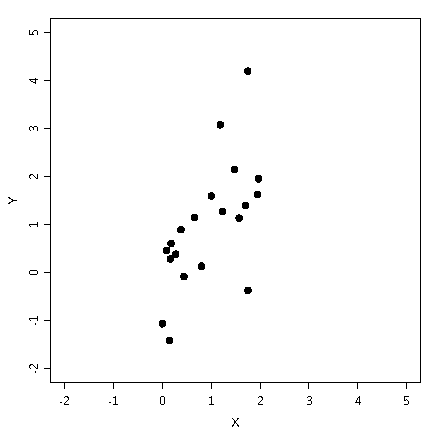
\includegraphics{Resources/Plots/KQIllu1-1} \end{center}
\normalsize
\end{frame}

\begin{frame}{Visualisierung KQ Schätzer}
\protect\hypertarget{visualisierung-kq-schuxe4tzer-1}{}
\footnotesize
\begin{center}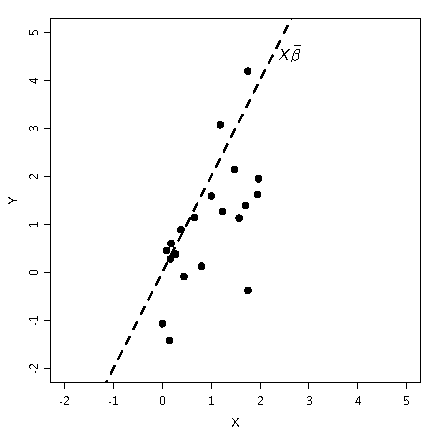
\includegraphics{Resources/Plots/KQIllu2-1} \end{center}
\normalsize
\end{frame}

\begin{frame}{Visualisierung KQ Schätzer}
\protect\hypertarget{visualisierung-kq-schuxe4tzer-2}{}
\footnotesize
\begin{center}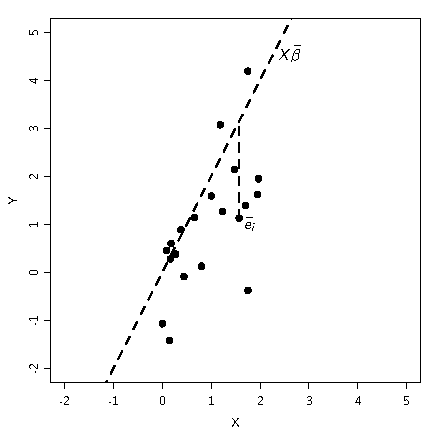
\includegraphics{Resources/Plots/KQIllu3-1} \end{center}
\normalsize
\end{frame}

\begin{frame}{Visualisierung KQ Schätzer}
\protect\hypertarget{visualisierung-kq-schuxe4tzer-3}{}
\footnotesize
\begin{center}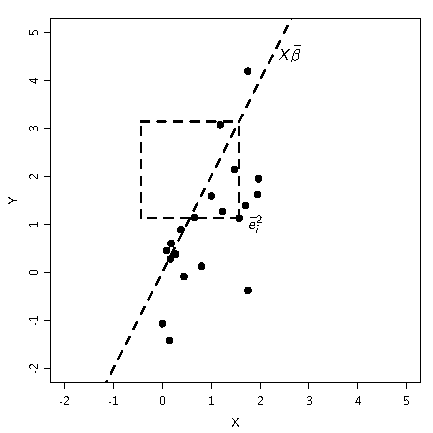
\includegraphics{Resources/Plots/KQIllu4-1} \end{center}
\normalsize
\end{frame}

\begin{frame}{Visualisierung KQ Schätzer}
\protect\hypertarget{visualisierung-kq-schuxe4tzer-4}{}
\footnotesize
\begin{center}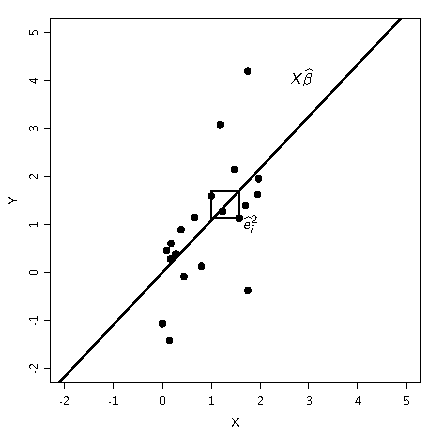
\includegraphics{Resources/Plots/KQIllu5-1} \end{center}
\normalsize
\end{frame}

\begin{frame}{Visualisierung KQ Schätzer}
\protect\hypertarget{visualisierung-kq-schuxe4tzer-5}{}
\footnotesize
\begin{center}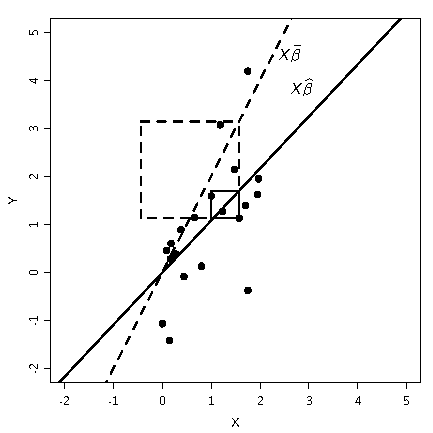
\includegraphics{Resources/Plots/KQIllu6-1} \end{center}
\normalsize
\end{frame}

\begin{frame}{KQ Schätzer in \R}
\protect\hypertarget{kq-schuxe4tzer-in}{}
\xmpl[Card (1995)]\label{ex:Card}

\begin{itemize}
\tightlist
\item
  Betrachten Sie die Lohnregression von Card (1995) \[
   \log(wage) = \beta_0+\beta_1\cdot educ + e.
   \]

  \begin{itemize}
  \tightlist
  \item
    Hier: \(\log(wage)=\) \alert{logarithmiertes Gehalt}, \(educ=\)
    \alert{Jahre in Ausbildung}.
  \end{itemize}
\item
  Die folgende Grafik zeigt die geschätzte Regressionsgerade \[
  \widehat{\log(wage)}=\widehat{\beta}_0 + \widehat{\beta}_1\cdot educ = 5.57 + 0.052\cdot educ.
  \]

  \begin{itemize}
  \tightlist
  \item
    Leute mit 1 zusätzlichem Jahr in Ausbildung verdienen im Schnitt
    5.2\% mehr Geld.
  \end{itemize}
\item
  \alert{Bemerke:} Obiges lineare Projektionsmodell kann auch als
  \alert{lineares bedingtes Erwartungswertmodell} interpretiert werden
  (so dass \(e=\epsilon\)).
\item
  \alert{Aber:} Jahre in Ausbildung sind sicher nicht unabhängig von
  weiteren unbeobachtbaren Faktoren in \(e\) (z.B.~Fähigkeit), also
  \(\E[e\mid educ]=0\) verletzt, und Interpretation als wahrer DGP
  ungültig (so dass \(e\neq u\)).
\end{itemize}

\endxmpl
\end{frame}

\begin{frame}[fragile]{KQ Schätzer in \R}
\protect\hypertarget{kq-schuxe4tzer-in-1}{}
\footnotesize

\begin{Shaded}
\begin{Highlighting}[]
\NormalTok{card }\OtherTok{\textless{}{-}} \FunctionTok{read\_dta}\NormalTok{(}\StringTok{"Resources/Card1995/Card1995.dta"}\NormalTok{)    }\CommentTok{\# Daten auf moodle oder Buch HP}
\NormalTok{ols  }\OtherTok{\textless{}{-}} \FunctionTok{lm}\NormalTok{(lwage76 }\SpecialCharTok{\textasciitilde{}}\NormalTok{ ed76, }\AttributeTok{data=}\NormalTok{card)                  }\CommentTok{\# KQ Schätzung}
\FunctionTok{summary}\NormalTok{(ols)}
\end{Highlighting}
\end{Shaded}

\begin{verbatim}
## 
## Call:
## lm(formula = lwage76 ~ ed76, data = card)
## 
## Residuals:
##     Min      1Q  Median      3Q     Max 
## -1.7380 -0.2776  0.0237  0.2884  1.4608 
## 
## Coefficients:
##             Estimate Std. Error t value Pr(>|t|)    
## (Intercept)  5.57088    0.03883   143.5   <2e-16 ***
## ed76         0.05209    0.00287    18.1   <2e-16 ***
## ---
## Signif. codes:  0 '***' 0.001 '**' 0.01 '*' 0.05 '.' 0.1 ' ' 1
## 
## Residual standard error: 0.421 on 3008 degrees of freedom
##   (603 observations deleted due to missingness)
## Multiple R-squared:  0.0987, Adjusted R-squared:  0.0984 
## F-statistic:  330 on 1 and 3008 DF,  p-value: <2e-16
\end{verbatim}

\normalsize
\end{frame}

\begin{frame}[fragile]{KQ Schätzer in \R}
\protect\hypertarget{kq-schuxe4tzer-in-2}{}
\footnotesize

\begin{Shaded}
\begin{Highlighting}[]
\FunctionTok{plot}\NormalTok{(lwage76 }\SpecialCharTok{\textasciitilde{}}\NormalTok{ ed76, }\AttributeTok{data =}\NormalTok{ card)                      }\CommentTok{\# plotte Resultate}
\FunctionTok{abline}\NormalTok{(ols, }\AttributeTok{col=}\StringTok{"blue"}\NormalTok{)                                }\CommentTok{\# mit Regressionsgerade als Vergleich}
\end{Highlighting}
\end{Shaded}

\begin{center}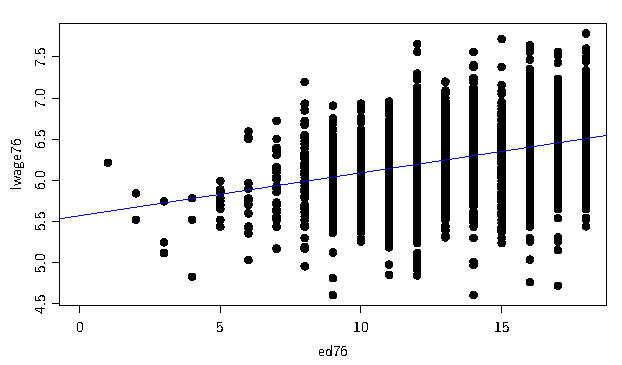
\includegraphics{Resources/Plots/KQinR2-1} \end{center}
\normalsize
\end{frame}

\begin{frame}{Matrixnotation}
\protect\hypertarget{matrixnotation}{}
\begin{itemize}
\tightlist
\item
  \alert{Matrixnotation} erlaubt uns oft eine übersichtlichere
  Schreibweise: \begin{equation}\label{eq:Matrixnotation}
  \underset{(n\times1)}{\mY}=\underset{(n\times k)}{\mX}\underset{(k\times1)}{\vbeta}+\underset{(n\times1)}{\ve},
  \end{equation} wobei \begin{equation*}
  \mY = \begin{pmatrix}Y_1\\ \vdots\\ Y_n \end{pmatrix},\qquad \mX=\begin{pmatrix}X_1^\prime\\ \vdots\\ X_n^\prime \end{pmatrix},\qquad\vbeta=\begin{pmatrix}\beta_1\\ \vdots\\ \beta_k \end{pmatrix},\qquad \ve=\begin{pmatrix}e_1\\ \vdots\\ e_n \end{pmatrix}.
  \end{equation*}
\item
  Insbesondere lassen sich auch \alert{Summen} einfacher darstellen: \[
  \sum_{i=1}^{n}X_i X_i^\prime=\mX^\prime\mX,\qquad\sum_{i=1}^{n}X_i Y_i=\mX^\prime\mY.
  \]
\item
  Damit \begin{equation}\label{eq:beta hat mat}
  \boxed{\ \widehat{\vbeta}=(\mX^\prime\mX)^{-1}\mX^\prime\mY.\ }
  \end{equation}
\end{itemize}
\end{frame}

\begin{frame}{Positive Definitheit}
\protect\hypertarget{positive-definitheit}{}
\begin{itemize}
\tightlist
\item
  Die Annahme aus Theorem~\ref{thm:KQ}, dass \(\mX^\prime\mX\) positiv
  definit ist, lässt sich weiter \alert{veranschaulichen}.
\item
  Weil \(\mX^\prime\mX\) symmetrisch ist, implizieren
  Propositionen~\zref{S-relprop3}.\zref{S-it:27.5}/\zref{S-it:27.6},
  \zref{S-rules3}.\zref{S-it:21.6},
  \zref{S-rules2}.\zref{S-it:20.8}/\zref{S-it:20.9}
  \begin{equation}\label{eq:equiv pd rk}
  \mX^\prime\mX\ \text{positiv definit}\qquad \Longleftrightarrow\qquad \mX\ \text{hat vollen Rang}. 
  \end{equation}
\item
  Vollen Rang zu haben heißt, dass die Spalten von
  \(\mX=(\vx_1\,|\, \ldots\,|\, \vx_k)=\) linear unabhängig sind (siehe
  Definition~\zref{S-linindep}), d.h. \[
  \sum_{i=1}^{k}c_i\vx_i=\vzero\qquad\Longrightarrow\qquad c_1=\ldots=c_k=0.
  \]
\item
  M.a.W.~hat \(\mX\) nicht vollen Rang (und \(\mX^\prime\mX\) ist damit
  nicht positiv definit), wenn man einen Regressor als Linearkombination
  der anderen schreiben kann, wie in \[
  \vx_j=-\sum_{i\neq j}\frac{c_i}{c_j}\vx_i.
  \]
\item
  In diesem Fall liegt \hil{Multikollinearität} vor.
\end{itemize}
\end{frame}

\begin{frame}{Positive Definitheit}
\protect\hypertarget{positive-definitheit-1}{}
\xmpl
\begin{itemize}
\item Betrachte das volle \hil{Dummy-Variablen} Modell:
\[
  \log(wage)=\beta_1+\beta_2\cdot man + \beta_3\cdot woman + e.
\]
\item Hier liegt \alert{Multikollinearität} vor, da $man + woman = 1$.
\item \alert{Lösung:} Lasse Konstante oder einen der Dummies weg.

\item \alert{Obacht:} Je nachdem was Sie machen, ändert sich Interpretation der Koeffizienten.

\begin{itemize}

\item Weglassen von Konstante führt zu
  \[
    \E\big[\log(wage)\mid woman=1\big]=\beta_3,
  \]
  so dass $\beta_3=$ Durchschnittslohn von Frauen.
\item Weglassen von $man$ führt zu
\[
  \E\big[\log(wage)\mid woman=1\big]=\beta_1 + \beta_3,
\]
so dass $\beta_1+\beta_3=$ Durchschnittslohn von Frauen.
\end{itemize}
\end{itemize}
\endxmpl
\end{frame}

\begin{frame}{Überblick}
\protect\hypertarget{uxfcberblick-8}{}
\begin{itemize}
\tightlist
\item
  KQ Schätzer
\item
  \textbf{Residuen, angepasste Werte, Projektions- und
  Residuenmachermatrix}
\item
  Frisch--Waugh--Lovell Theorem
\item
  Anpassungsmaße
\end{itemize}
\end{frame}

\begin{frame}{Terminologie}
\protect\hypertarget{terminologie}{}
\begin{itemize}
\tightlist
\item
  Wir führen weitere wichtige \alert{Grundbegriffe} ein, die im
  Zusammenhang mit dem linearen Projektionsmodell immer wieder
  auftauchen.
\end{itemize}

\defn\label{defn:Aw and Resids} Die \hil{angepassten Werte} und
\hil{Residuen} sind \begin{align*}
    \widehat{\mY} &= \mX\widehat{\vbeta},\\
    \widehat{\ve} &= \mY- \widehat{\mY}.
  \end{align*} Die \hil{Projektionsmatrix} und
\hil{Residuenmachermatrix} sind \begin{align*}
    \mP &:= \mP_{\mX}:=\mX(\mX^\prime\mX)^{-1}\mX^\prime,\\
    \mM &:= \mM_{\mX}:=\mI-\mP.
  \end{align*} \enddefn

\begin{itemize}
\tightlist
\item
  \(\mP\) heißt Projektionsmatrix und \(\mM\) Residuenmachermatrix, weil
  \begin{align}
  \widehat{\mY} &= \mX\widehat{\vbeta} = \mX(\mX^\prime\mX)^{-1}\mX^\prime\mY=\mP\mY,\notag\\
  \widehat{\ve} &= \mY- \widehat{\mY} = (\mI-\mP)\mY=\mM\mY.\label{eq:e hat why}
  \end{align}
\end{itemize}
\end{frame}

\begin{frame}{Visualisierung in \R}
\protect\hypertarget{visualisierung-in}{}
\framesubtitle{Lineare Projektion von Baumvolumen auf Umfang und Höhe}

\footnotesize
\begin{center}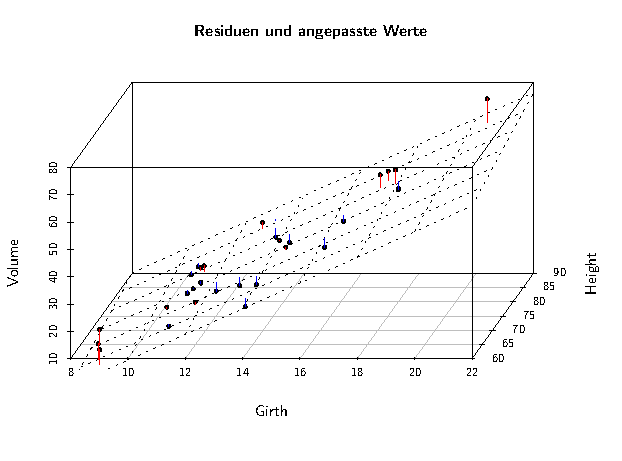
\includegraphics{Resources/Plots/RegPlane-1} \end{center}
\normalsize
\end{frame}

\begin{frame}{Projektionsmatrix}
\protect\hypertarget{projektionsmatrix}{}
\thmn[Eigenschaften von $\mP$ (Hansen, 2022, Theorem 3.3)]\label{thm:Eig P}
Wenn \(\mX^\prime\mX\) p.d.~ist, dann gilt

\begin{enumerate}
  \item\label{it:P1} $\mP\mX=\mX$.
  \item\label{it:P2} $\mP$ ist \hil{symmetrisch}, d.h.\ $\mP=\mP^\prime$.
  \item\label{it:P3} $\mP$ ist \hil{idempotent}, d.h.\ $\mP=\mP\mP$.
  \item\label{it:P4} $\tr(\mP)=k$.
  \item\label{it:P5} Die Eigenwerte von $\mP$ sind $0$ und $1$.
  \item\label{it:P6} $\mP$ hat $k$ Eigenwerte gleich $1$ und $n-k$ gleich $0$.
  \item\label{it:P7} $\rk(\mP)=k$.
\end{enumerate}
\endthmn
\end{frame}

\begin{frame}{Projektionsmatrix}
\protect\hypertarget{projektionsmatrix-1}{}
\begin{block}{Beweis von Theorem \ref{thm:Eig P}}
\begin{enumerate}
  \item Per Definition gilt $\mP\mX=\mX(\mX^\prime\mX)^{-1}\mX^\prime\mX=\mX$.
  \item Symmetrie gilt, da
\begin{eqnarray*}
  \mP^\prime &=& \big[\mX(\mX^\prime\mX)^{-1}\mX^\prime\big]^\prime\\
  &\overset{\text{Prop. }\zref{S-rules2}.\zref{S-it:20.4}}{=}& (\mX^\prime)^\prime\big((\mX^\prime\mX)^{-1}\big)^\prime\mX^\prime\\
  &\overset{\text{Prop. }\zref{S-rules3}.\zref{S-it:21.3}}{=}& \mX\big((\mX^\prime\mX)^\prime\big)^{-1}\mX^\prime\\
  &\overset{\text{Prop. }\zref{S-rules2}.\zref{S-it:20.4}}{=}& \mX(\mX^\prime\mX)^{-1}\mX^\prime=\mP.
\end{eqnarray*}

\item $\mP\mP=\mP\mX(\mX^\prime\mX)^{-1}\mX^\prime\overset{\ref{it:P1}}{=}\mX(\mX^\prime\mX)^{-1}\mX^\prime=\mP$.

\item $\tr(\mP)=\tr\big(\mX(\mX^\prime\mX)^{-1}\mX^\prime\big)\overset{\text{Prop.}}{\underset{\zref{S-rules2}.\zref{S-it:20.6}}{=}}\tr\big((\mX^\prime\mX)^{-1}\mX^\prime\mX\big)=\tr(\mI)=k$.

\item Folgt aus Proposition\ \zref{S-relprop3}.\zref{S-it:27.3} und Idempotenz von $\mP$ (siehe \ref{it:P3}).

\item -- \textcolor{dueblue}{7.} selber machen.
\end{enumerate}

\end{block}
\end{frame}

\begin{frame}{Projektionsmatrix}
\protect\hypertarget{projektionsmatrix-2}{}
\xmpl[Transformierte Regressoren]

\begin{itemize}
  \item Wir \alert{transformieren} die Regressoren $\mX$ mit invertierbarer $(k\times k)$-Matrix $\mA$ zu $\mX\mA$.
    \begin{itemize}
      \item Z.B.\ ändern der Einheit von Metern zu Zentimetern, Celsius zu Fahrenheit etc.
    \end{itemize}
  \item \alert{Frage:} Was passiert mit den angepassten Werten und Residuen?
  \item \alert{Antwort:} Nichts, denn die Projektionsmatrix bleibt dieselbe:
  \begin{eqnarray*}
    \mP_{\mX\mA} &=& \mX\mA\big((\mX\mA)^\prime\mX\mA\big)^{-1}(\mX\mA)^\prime\\
    &\overset{\text{Prop. }\zref{S-rules2}.\zref{S-it:20.4}}{=} & \mX\mA(\mA^\prime\mX^\prime\mX\mA)^{-1}\mA^\prime\mX^\prime\\
    &\overset{\text{Prop. }\zref{S-rules2}.\zref{S-it:20.5}}{=} & \mX\mA\mA^{-1}(\mX^\prime\mX)^{-1}(\mA^\prime)^{-1}\mA^\prime\mX^\prime \\
    &=&\mP.
  \end{eqnarray*}
  \item \alert{Nebenbemerkung:} $\widehat{\vbeta}$ ändert sich natürlich...
\end{itemize}
\endxmpl
\end{frame}

\begin{frame}{Projektionsmatrix}
\protect\hypertarget{projektionsmatrix-3}{}
\xmpl[*]

\begin{itemize}
  \item Es gilt:
  \begin{eqnarray*}
  \widehat{\vbeta}_{\mX\mA} &=& (\mA^\prime\mX^\prime\mX\mA)^{-1}\mA^\prime\mX^\prime\mY\\
  &\overset{\text{Prop. }\zref{S-rules2}.\zref{S-it:20.5}}{=} & \mA^{-1}(\mX^\prime\mX)^{-1}(\mA^\prime)^{-1}\mA^\prime\mX^\prime\mY\\
  &=& \mA^{-1}(\mX^\prime\mX)^{-1}\mX^\prime\mY\\
  &=& \mA^{-1}\widehat{\vbeta}.
  \end{eqnarray*}
  \item Wäre also 
  \[
    \mA=\begin{pmatrix}1/12 & 0 \\ 0 & 100\end{pmatrix},\quad\text{so dass}\quad \mA^{-1}=\begin{pmatrix}12 & 0 \\ 0 & 1/100\end{pmatrix},
  \]
  wird der Effekt der Änderung in den Regressoren intuitiv angepasst.
\end{itemize}
\endxmpl
\end{frame}

\begin{frame}{Residuenmachermatrix}
\protect\hypertarget{residuenmachermatrix}{}
\begin{itemize}
\tightlist
\item
  Viele der Eigenschaften von \(\mP\) aus Theorem \ref{thm:Eig P} gelten
  ähnlich auch für \(\mM\):
\end{itemize}

\thmn[Eigenschaften von $\mM$]\label{thm:Eig M} Wenn \(\mX^\prime\mX\)
p.d.~ist, dann gilt

\begin{enumerate}
  \item\label{it:M1} $\mM\mX=\vzero$.
  \item\label{it:M2} $\mM$ ist symmetrisch.
  \item\label{it:M3} $\mM$ ist idempotent.
  \item\label{it:M4} $\tr(\mM)=n-k$.
  \item\label{it:M5} Die Eigenwerte von $\mM$ sind $0$ und $1$.
  \item\label{it:M6} $\mM$ hat $n-k$ Eigenwerte gleich $1$ und $k$ gleich $0$.
  \item\label{it:M7} $\rk(\mM)=n-k$.
\end{enumerate}
\endthmn
\end{frame}

\begin{frame}{Angepasste Werte und Residuen}
\protect\hypertarget{angepasste-werte-und-residuen}{}
\thmn[Orthogonalität]\label{thm:ortho} Wenn \(\mX^\prime\mX\) p.d.~ist,
dann gelten \begin{align}
  \mX^\prime\widehat{\ve}&=\vzeros,\label{eq:X e.hat}\\
  \widehat{\mY}^\prime\widehat{\ve}&=0.\label{eq:Y.hat e.hat}
\end{align} \endthmn

\begin{itemize}
\tightlist
\item
  \eqref{eq:X e.hat} bedeutet: Regressoren und Residuen sind
  \hil{orthogonal} zueinander.

  \begin{itemize}
  \tightlist
  \item
    Wenn \(\mX\) eine Konstante beinhaltet, folgt insbesondere
    \(0=\sum_{i=1}^{n}\widehat{e}_i\), d.h.~das Stichprobenmittel der
    \(\widehat{\ve}\) ist Null.
  \end{itemize}
\item
  \eqref{eq:Y.hat e.hat} bedeutet: Angepasste Werte und Residuen sind
  orthogonal zueinander.

  \begin{itemize}
  \tightlist
  \item
    Letzteres impliziert, dass KQ \(\mY\) in
    \alert{zwei orthogonale Komponenten zerlegt:}
    \begin{equation}\label{eq:Zerl fit resid}
    \mY=\mP\mY + \mM\mY = \widehat{\mY} + \widehat{\ve}.
    \end{equation}
  \end{itemize}
\end{itemize}
\end{frame}

\begin{frame}{Angepasste Werte und Residuen}
\protect\hypertarget{angepasste-werte-und-residuen-1}{}
\footnotesize
\begin{center}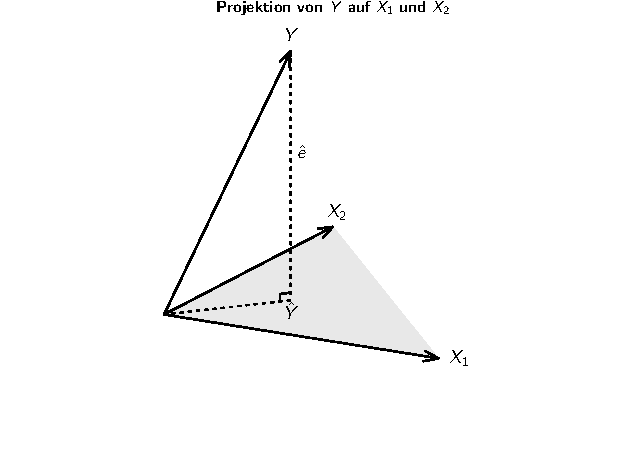
\includegraphics{Resources/Plots/Illu-1} \end{center}
\normalsize
\end{frame}

\begin{frame}{Angepasste Werte und Residuen}
\protect\hypertarget{angepasste-werte-und-residuen-2}{}
\begin{block}{Beweis von Theorem \ref{thm:ortho}}
\eqref{eq:X e.hat} folgt direkt aus
\begin{eqnarray*}
  \mX^\prime\widehat{\ve}&=&\mX^\prime\mM\mY\\
  &\overset{\text{Thm.\ \ref{thm:Eig M}.\ref{it:M2}}}{=}&\mX^\prime\mM^\prime\mY\\
  &\overset{\text{Prop. }\zref{S-rules2}.\zref{S-it:20.4}}{=}&(\mM\mX)^\prime\mY\\
  &\overset{\text{Thm.\ \ref{thm:Eig M}.\ref{it:M1}}}{=}&\vzero.
\end{eqnarray*}
\eqref{eq:Y.hat e.hat} folgt direkt aus
\begin{eqnarray*}
  \widehat{\mY}^\prime\widehat{\ve} &=& (\mP\mY)^\prime(\mM\mY)\\
  &=&\mY^\prime\mathcolor{red}{\mP\mM}\mY\\
  &=&\mY^\prime\mathcolor{red}{\mP(\mI-\mP)}\mY\\
   &=&\mY^\prime\mathcolor{red}{(\mP-\mP\mP)}\mY\\
   &\overset{\text{Thm.\ \ref{thm:Eig P}.\ref{it:P3}}}{=}&\mY^\prime\mathcolor{red}{(\mP-\mP)}\mY\\
  &=&\vzero.
\end{eqnarray*}
\end{block}
\end{frame}

\begin{frame}{Überblick}
\protect\hypertarget{uxfcberblick-9}{}
\begin{itemize}
\tightlist
\item
  KQ Schätzer
\item
  Residuen, angepasste Werte, Projektions- und Residuenmachermatrix
\item
  \textbf{Frisch--Waugh--Lovell Theorem}
\item
  Anpassungsmaße
\end{itemize}
\end{frame}

\begin{frame}{FWL Theorem}
\protect\hypertarget{fwl-theorem}{}
\begin{itemize}
\tightlist
\item
  Eine weitere nützliche \alert{Interpretation} der geschätzten
  Regressionskoeffizienten liefert das so genannte
  \hil{Frisch--Waugh--Lovell (FWL) Theorem}.
\item
  Um dies zu formulieren, \alert{partitioniere}
  \(\mX=(\mX_1\mid \mX_2)\) und schreibe das lineare Modell zu
  \begin{equation}\label{eq:part LM}
  \mY=\underset{(n\times k_1)}{\mX_1}\vbeta_1+\underset{(n\times k_2)}{\mX_2}\vbeta_2+\ve.
  \end{equation}
\end{itemize}

\thmn[FWL Theorem]\label{thm:FWL} Der Schätzer \(\widehat{\vbeta}_2\)
und die Residuen \(\widehat{\ve}\) können entweder durch KQ Schätzung
von \eqref{eq:part LM} berechnet werden oder -- \alert{äquivalent} --
durch folgenden Algorithmus:

\begin{enumerate}
  \item\label{eq:FWL1} Regressiere $\mY$ auf $\mX_1$, erhalte die Residuen $\widetilde{\mY}=\mM_{\mX_1}\mY$.
  \item\label{eq:FWL2} Regressiere $\mX_2$ auf $\mX_1$, erhalte die Residuen $\widetilde{\mX}_2=\mM_{\mX_1}\mX_2$.
  \item\label{eq:FWL3} Regressiere $\widetilde{\mY}$ auf $\widetilde{\mX}_2$, erhalte den KQ Schätzer $\widehat{\vbeta}_2$ und die Residuen $\widehat{\ve}$.
\end{enumerate}
\endthmn

\begin{itemize}
\tightlist
\item
  \alert{Intuition:} \(\widehat{\vbeta}_2\) schätzt Effekt von \(\mX_2\)
  auf \(\mY\) nachdem aus beiden der (lineare) Effekt von \(\mX_1\)
  \alert{herausgerechnet} wurde.
\end{itemize}
\end{frame}

\begin{frame}{FWL Theorem}
\protect\hypertarget{fwl-theorem-1}{}
\begin{block}{Beweis von Theorem \ref{thm:FWL} (1/3)}
Der KQ Schätzer aus dem Algorithmus ergibt sich nach Standard KQ Formel zu
\begin{align}
  \widehat{\vbeta}_2 &= (\widetilde{\mX}_2^\prime \widetilde{\mX}_2)^{-1} \widetilde{\mX}_2^\prime\widetilde{\mY}\\
  &= (\underbrace{\mX_2^\prime\mM_{\mX_1}^\prime}_{"\mX^\prime"}\underbrace{\mM_{\mX_1}\mX_2}_{"\mX"})^{-1}\underbrace{\mX_2^\prime\mM_{\mX_1}^\prime}_{"\mX^\prime"}\underbrace{\mM_{\mX_1}\mY}_{"\mY"}\notag\\
  &= (\mX_2^\prime\mM_{\mX_1}\mX_2)^{-1}\mX_2^\prime\mM_{\mX_1}\mY,\label{eq:(2.15)}
\end{align}
wobei der letzte Schritt aus Theorem \ref{thm:Eig M}.\ref{it:M2} und \ref{thm:Eig M}.\ref{it:M3} folgt.\medskip

Wir zeigen jetzt, dass der \alert{Standard KQ Schätzer} genau \eqref{eq:(2.15)} erfüllt. Mit \eqref{eq:e hat why} folgt
\begin{align}
  \mY &= \mX\widehat{\vbeta}+\mM\mY\notag\\
    &= \mX_1\widehat{\vbeta}_1 + \mX_2\widehat{\vbeta}_2+\mM\mY.\label{eq:h0}
\end{align}
Durchmultiplizieren von \eqref{eq:h0} mit $\mX_2^\prime\mM_{\mX_1}$ ergibt (ausnutzend, dass $\mM_{\mX_1}\mX_1=\vzero$)
\begin{equation}\label{eq:(2.17)}
\mX_2^\prime\mM_{\mX_1}\mY = \mX_2^\prime\mM_{\mX_1}\mX_2\widehat{\vbeta}_2 + \mX_2^\prime\mM_{\mX_1}\mM\mY.
\end{equation}
\end{block}
\end{frame}

\begin{frame}{FWL Theorem}
\protect\hypertarget{fwl-theorem-2}{}
\begin{block}{Beweis von Theorem \ref{thm:FWL} (2/3)}
Zeigen nun: Letzter Term in \eqref{eq:(2.17)} ist gleich Null, d.h.\ $\mX_2^\prime\mM_{\mX_1}\mM\mY=\vzero$.\medskip

Schreibe dafür $\mP\mX=\mX$ (Theorem \ref{thm:Eig P}.\ref{it:P1}) partitioniert als $\mP(\mX_1\mid\mX_2)=(\mX_1\mid\mX_2)$, um zu erkennen, dass $\mathcolor{red}{\mP\mX_1}=\mathcolor{red}{\mX_1}$. Damit:
\[
  \mP\mP_{\mX_1}=\mathcolor{red}{\mP\mX_1}(\mX_1^\prime\mX_1)^{-1}\mX_1^\prime = \mathcolor{red}{\mX_1}(\mX_1^\prime\mX_1)^{-1}\mX_1^\prime=\mP_{\mX_1}.
\]
Wegen Symmetrie von $\mP$ und $\mP_{\mX_1}$ (Theorem\nbs{}\ref{thm:Eig P}.\ref{it:P2}) daher $\mP_{\mX_1}\mP=\mP_{\mX_1}$, womit
\begin{align}
\mM_{\mX_1}\mM &= (\mI-\mP_{\mX_1})(\mI-\mP)\notag\\
&= \mI-\mP-\mP_{\mX_1}+\mP_{\mX_1}\mP\notag\\
&= \mI-\mP-\mP_{\mX_1}+\mP_{\mX_1}\notag\\
&=\mI-\mP\notag\\
&=\mM.\label{eq:help MM}
\end{align}
Damit und weil $\mM\mX_2=\vzero$ (aus Theorem \ref{thm:Eig M}.\ref{it:M1}):
\begin{equation}\label{eq:(2.18)}
  \mX_2^\prime\mM_{\mX_1}\mM\overset{\eqref{eq:help MM}}{=}\mX_2^\prime\mM\overset{\text{Prop. }\zref{S-rules2}.\zref{S-it:20.4}}{=}(\mM^\prime\mX_2)^\prime\overset{\text{Thm. \ref{thm:Eig M}.\ref{it:M2}}}{=}(\mM\mX_2)^\prime=\vzero.
\end{equation}

\end{block}
\end{frame}

\begin{frame}{FWL Theorem}
\protect\hypertarget{fwl-theorem-3}{}
\begin{block}{Beweis von Theorem \ref{thm:FWL} (3/3)}
Einsetzen von \eqref{eq:(2.18)} in \eqref{eq:(2.17)} ergibt:
\[
  \mX_2^\prime\mM_{\mX_1}\mY=\mX_2^\prime\mM_{\mX_1}\mX_2\widehat{\vbeta}_2.
\]
Auflösen nach $\widehat{\vbeta}_2$ liefert den Schätzer in \eqref{eq:(2.15)} und wir sind fertig.\medskip

Jetzt zu den \alert{Residuen:} Durchmultiplizieren von \eqref{eq:h0} mit $\mM_{\mX_1}$ liefert (da $\mM_{\mX_1}\mM=\mM$)
\begin{align*}
  \mM_{\mX_1}\mY &= \mM_{\mX_1}\mX_2\widehat{\vbeta}_1 + \mM\mY\\
  \Longleftrightarrow\qquad \widetilde{\mY} &= \widetilde{\mX}_2\widehat{\vbeta}_2 + \mM\mY.
\end{align*}
Da (nach obigem) $\widehat{\vbeta}_2$ der Schätzer einer Regression von $\widetilde{\mY}$ auf $\widetilde{\mX}_2$ ist, sind $\mM\mY$ genau die Regressionsresiduen (wegen \eqref{eq:Zerl fit resid}). Aber es gilt ja genau $\widehat{\ve}=\mM\mY$ nach \eqref{eq:e hat why}!

\end{block}
\end{frame}

\begin{frame}{Anwendung des FWL Theorems}
\protect\hypertarget{anwendung-des-fwl-theorems}{}
\xmpl[Regression mit Konstante]\label{ex:FWL}

\begin{itemize}
  \item Nehme $\mX_1=\viota=(1,\ldots,1)^\prime$. Folgende Regressionen ergeben nach dem FWL Theorem identische Schätzungen $\widehat{\vbeta}_2$ für den Effekt von $\mX_2$:
  \begin{enumerate}
    \item Regressiere $\mY$ auf $\viota$ (d.h.\ eine Konstante) und $\mX_2$.
    \item Regressiere $\mY-\overline{\mY}$ auf $\mX_2-\overline{\mX}_2$, wobei letzteres die Spalten von $\mX_2$ zentriert um deren jeweilge Spaltenmittelwerte.
  \end{enumerate}
  \item Gilt, weil
  \[
    \mM_{\viota} = \mI-\viota(\viota^\prime\viota)^{-1}\viota^\prime=\mI-\frac{\viota\viota^\prime}{n}.
  \]
  \item Daher sind die Residuen aus Schritt \ref{eq:FWL1} des FWL Theorems
  \[
    \widetilde{\mY}=\mM_{\viota}\mY=\mY-\viota \frac{1}{n}\viota^\prime \mY=\mY-\viota\overline{Y}=:\mY-\overline{\mY}
  \]
  die \hil{mittelwertbereinigten} Variablen.
  
  \item Ähnliches gilt für Residuen $\widetilde{\mX}_2=\mM_{\iota}\mX_2=\mX_2-\overline{\mX}_2$ aus Schritt \ref{eq:FWL2} des FWL Theorems.
\end{itemize}
\endxmpl
\end{frame}

\begin{frame}{Überblick}
\protect\hypertarget{uxfcberblick-10}{}
\begin{itemize}
\tightlist
\item
  KQ Schätzer
\item
  Residuen, angepasste Werte, Projektions- und Residuenmachermatrix
\item
  Frisch--Waugh--Lovell Theorem
\item
  \textbf{Anpassungsmaße}
\end{itemize}
\end{frame}

\begin{frame}{TSS, ESS und SSR}
\protect\hypertarget{tss-ess-und-ssr}{}
\begin{itemize}
\tightlist
\item
  \eqref{eq:Y.hat e.hat} (also \(\widehat{\mY}^\prime\widehat{\ve}=0\))
  erlaubt uns die \hil{Total Sum of Squares}
  \(\text{TSS}=\mY^\prime\mY\) zu zerlegen in \begin{align*}
  \mY^\prime\mY &= (\widehat{\mY} + \widehat{\ve})^\prime(\widehat{\mY} + \widehat{\ve})\\
  &= \widehat{\mY}^\prime\widehat{\mY} + 2\widehat{\mY}^\prime\widehat{\ve}+\widehat{\ve}^\prime\widehat{\ve}\\
  &= \widehat{\mY}^\prime\widehat{\mY} + \widehat{\ve}^\prime\widehat{\ve}\\
  &=: \text{ESS} + \text{SSR},
  \end{align*} wobei ESS die \hil{Explained Sum of Squares} sind und SSR
  die \hil{Sum of Squared Residuals}.
\item
  Das ist eine \alert{fundamentale Eigenschaft} der KQ Schätzung: KQ
  zerlegt Varianz von \(\mY\)

  \begin{enumerate}
  \tightlist
  \item
    in einen Teil, den wir \alert{erklären} können, und
  \item
    in einen Teil, den wir \alert{nicht erklären} können.
  \end{enumerate}
\end{itemize}
\end{frame}

\begin{frame}{Unzentriertes \(R^2\)}
\protect\hypertarget{unzentriertes-r2}{}
\begin{itemize}
\tightlist
\item
  Die obige Zerlegung \(\text{TSS}=\text{ESS} + \text{SSR}\) motiviert
  das \hil{unzentrierte $R^2$} als \alert{Maß für die Anpassungsgüte:}
\end{itemize}

\defn[\hil{Unzentriertes $R^2$}]\[
  R_u^2=\frac{\text{ESS}}{\text{TSS}}=\frac{\text{TSS}-\text{SSR}}{\text{TSS}}=1-\frac{\text{SSR}}{\text{TSS}}=1-\frac{\widehat{\ve}^\prime\widehat{\ve}}{\mY^\prime\mY}.
\] \enddefn

\begin{itemize}
\tightlist
\item
  Wir interpretieren \(R_u^2\) als den Teil der Variation in den Daten,
  der durch das Modell erklärt wird.

  \begin{itemize}
  \tightlist
  \item
    \(R_u^2=1\), wenn die Regressionslinie perfekt passt.
  \item
    \(R_u^2=0\), wenn \(\widehat{\vbeta}=\vzero\) (siehe
    \eqref{eq:Zerl fit resid} mit dann
    \(\mY=\mX\widehat{\vbeta} + \widehat{\ve}=\widehat{\ve}\)).
  \end{itemize}
\end{itemize}
\end{frame}

\begin{frame}{Zentriertes \(R^2\)}
\protect\hypertarget{zentriertes-r2}{}
\begin{itemize}
\tightlist
\item
  Das unzentrierte \(R^2\) wird \alert{selten benutzt}, da
  Lineartransformationen von \(\mY\) das \(R_u^2\) ändern.
\item
  Dieser Nachteil wir vermieden durch das \hil{zentrierte $R^2$}:
\end{itemize}

\defn[\hil{Zentriertes $R^2$}]\begin{eqnarray*}
  R^2 &=&1-\frac{\widehat{\ve}^\prime\widehat{\ve}}{\mY^\prime\mM_{\viota}\mY}\\
      &\overset{\text{Bsp.}\ \ref{ex:FWL}}{=}&1-\frac{\widehat{\ve}^\prime\widehat{\ve}}{(\mY-\overline{\mY})^\prime(\mY-\overline{\mY})}.
\end{eqnarray*} \enddefn

\begin{itemize}
\tightlist
\item
  \alert{Interpretation:} Modellanpassung wird verglichen mit
  Referenzmodell, welches nur Konstante enthält (so dass
  \(\widehat{\mY}^{\text{ref}}=\overline{\mY}\) und somit
  \(\widehat{\ve}^{\text{ref}}=\mY-\overline{\mY}\) wie in
  Beispiel~\ref{ex:FWL}).
\item
  \alert{Obacht:} Wenn angepasstes Modell keine Konstante enthält, ist
  \(R^2<0\) möglich -- etwas unnatürlich für ein \emph{Anpassungs}maß.
\end{itemize}
\end{frame}

\hypertarget{eigenschaften-von-kq-in-kleinen-stichproben}{%
\section{Eigenschaften von KQ in kleinen
Stichproben}\label{eigenschaften-von-kq-in-kleinen-stichproben}}

\begin{frame}{}
\protect\hypertarget{section-3}{}
\centerline{\textbf{Eigenschaften von KQ in kleinen Stichproben}}
\centerline{(Hansen, 2022, Kapitel 4)}
\end{frame}

\begin{frame}{Modell}
\protect\hypertarget{modell}{}
\begin{itemize}
\tightlist
\item
  In diesem Kapitel betrachten wir das
  \alert{lineare bedingte Erwartungswertmodell}
  \begin{equation}\label{eq:lbE}
  \boxed{\ Y=X^\prime\vbeta+e,\qquad\E[e\mid X]=0.\ }
  \end{equation}
\item
  Streng genommen sollten wir also \(Y=X^\prime\vbeta+\epsilon\),
  \(\E[\epsilon\mid X]=0\) schreiben, aber wir tun dies hier nicht, um
  die Notation einheitlich zu halten.

  \begin{itemize}
  \tightlist
  \item
    Seien Sie sich aber nach wie vor im Klaren über den Unterschied
    zwischen dem linearen \alert{Projektionsmodell} und dem linearen
    bedingten \alert{Erwartungswertmodell}!
  \end{itemize}
\item
  In diesem Kapitel leiten wir Verteilungseigenschaften von
  \(\widehat{\vbeta}\) her, die in kleinen Stichproben --
  \alert{d.h.\ für jedes (!) $n$} -- gelten.
\end{itemize}
\end{frame}

\begin{frame}{Stichprobe}
\protect\hypertarget{stichprobe}{}
\begin{itemize}
\tightlist
\item
  Annahme~\ref{ass:id} ist nicht stark genug, um
  Verteilungseigenschaften von \(\widehat{\vbeta}\) herzuleiten, weshalb
  wir nachschärfen:\bigskip
\end{itemize}

\ass\label{ass:iid} Die Variablen \((Y_1,X_1),\ldots,(Y_n,X_n)\) sind
\hil{unabhängig, identisch verteilte (u.i.v.)} Ziehungen aus einer
gemeinsamen Verteilung \(F\). \endass

\begin{itemize}
\tightlist
\item
  \alert{Plausible} Annahme für Querschnittsdaten.

  \begin{itemize}
  \tightlist
  \item
    Wenn sie eine Zufallsstichprobe von 1000 Leuten aus einer großen
    Population (z.B.~Deutschland) ziehen, sollten die Antworten ungefähr
    unabhängig sein.
  \end{itemize}
\item
  \alert{Obacht:} Wenn Individuen in irgendeiner Art verbunden sind
  (z.B.~Schüler aus verschiedenen Parallelklassen), kann die
  Unabhängigkeitsannahme verletzt sein.
\item
  Damit der KQ Schätzer eindeutig ist, nehmen wir zudem an:
\end{itemize}

\ass\label{ass:pd} \(\mX^\prime\mX\) ist positiv definit. \endass
\end{frame}

\begin{frame}{Überblick}
\protect\hypertarget{uxfcberblick-11}{}
\begin{itemize}
\tightlist
\item
  \textbf{Erwartungswert}
\item
  Varianz
\item
  Gauss--Markov Theorem
\item
  Ausschluss und Inklusion von Variablen
\end{itemize}
\end{frame}

\begin{frame}{Erwartungswert}
\protect\hypertarget{erwartungswert}{}
\begin{itemize}
\tightlist
\item
  Ein \alert{Gütekriterium} eines Schätzers ist, dass er im Mittel
  richtig schätzt (a.k.a.~Unverzerrtheit):
\end{itemize}

\defn[Unverzerrtheit]Ein Schätzer \(\widehat{\vtheta}\) ist
\hil{unverzerrt} für \(\vtheta\), wenn
\(\E\big[\widehat{\vtheta}\big]=\vtheta\). \enddefn

\begin{itemize}
\tightlist
\item
  \alert{Frage:} Ist der KQ Schätzer \(\widehat{\vbeta}\) unverzerrt für
  \(\vbeta\)?
\end{itemize}

\thmn[Hansen (2022, Theorem 4.1)]\label{thm:cond exp ols} Im linearen
bedingten Erwartungswertmodell \eqref{eq:lbE} gilt unter den Annahmen
\ref{ass:1}, \ref{ass:iid} und \ref{ass:pd}, dass die bedingte
Verteilung \(\widehat{\vbeta}\mid\mX\) um \(\vbeta\) zentriert ist, d.h.
\[
  \E\big[\widehat{\vbeta}\mid \mX\big]=\vbeta.
\] \endthmn

\begin{itemize}
\tightlist
\item
  Theorem \ref{thm:cond exp ols} und das GIE implizieren die
  (unbedingte) \alert{Unverzerrtheit} des KQ Schätzers,
  d.h.~\(\E\big[\widehat{\vbeta}\big]=\vbeta\).
\end{itemize}
\end{frame}

\begin{frame}{Erwartungswert}
\protect\hypertarget{erwartungswert-1}{}
\begin{block}{Beweis von Theorem \ref{thm:cond exp ols}}
Unter Annahme \ref{ass:iid} gilt im linearen bedingten Erwartungswertmodell
\[
  \E[Y_i\mid X_1,\ldots,X_n]\overset{\text{ÜA}}{=}\E[Y_i\mid X_i]\overset{\eqref{eq:lbE}}{=}X_i^\prime\vbeta.
\]
Damit
\begin{equation}\label{eq:h1}
  \E[\mY\mid\mX]\overset{\text{Def.}}{=}\begin{pmatrix}\vdots\\ \E[Y_i\mid X_1,\ldots,X_n]\\ \vdots\end{pmatrix}=\begin{pmatrix}\vdots\\ X_i^\prime\vbeta\\ \vdots\end{pmatrix}=\mX\vbeta.
\end{equation}
Dies ausnutzend erhalten wir
\begin{eqnarray*}
 \E\big[\widehat{\vbeta}\mid \mX\big] &\overset{\eqref{eq:beta hat mat}}{=}& \E\big[(\mX^\prime\mX)^{-1}\mX^\prime\mY\mid\mX\big]\\
 &\overset{\eqref{eq:pull out}}{=}& (\mX^\prime\mX)^{-1}\mX^\prime\E\big[\mY\mid\mX\big]\\
 &\overset{\eqref{eq:h1}}{=}&(\mX^\prime\mX)^{-1}\mX^\prime\mX\vbeta\\
 &=&\vbeta.
\end{eqnarray*}
\end{block}
\end{frame}

\begin{frame}{Illustration der Unverzerrtheit in \R}
\protect\hypertarget{illustration-der-unverzerrtheit-in}{}
\xmpl[Simulationsbeispiel]

\begin{itemize}
\tightlist
\item
  Betrachte den DGP \[
  Y_i=\beta_0+e_i,\qquad i=1,\ldots,n
  \] mit \(e_i\overset{\text{u.i.v.}}{\sim}N(0,1)\), \(\beta_0=0\) und
  \(n=100\).
\item
  Der KQ Schätzer ist
  \(\widehat{\beta}_0=\frac{1}{n}\sum_{i=1}^{n}Y_i\).
\item
  Über verschiedene Replikationen \(\{Y_i^{(r)}\}_{i=1,\ldots,n}\)
  (\(r=1,\ldots,\text{reps}\)) hinweg, sollte für die KQ Schätzer
  \(\widehat{\beta}_0^{(r)}\) gelten: \[
  \frac{1}{\text{reps}}\sum_{r=1}^{\text{reps}}\widehat{\beta}_0^{(r)} \approx \E[\widehat{\beta}_0]=\beta_0.
  \]
\end{itemize}

\endxmpl
\end{frame}

\begin{frame}[fragile]{Illustration der Unverzerrtheit in \R}
\protect\hypertarget{illustration-der-unverzerrtheit-in-1}{}
\footnotesize

\begin{Shaded}
\begin{Highlighting}[]
\NormalTok{n    }\OtherTok{\textless{}{-}} \DecValTok{100}            \CommentTok{\# Stichprobenlänge}
\NormalTok{reps }\OtherTok{\textless{}{-}} \DecValTok{500}            \CommentTok{\# Anzahl Wiederholungen}
\NormalTok{KQ   }\OtherTok{\textless{}{-}} \FunctionTok{rep}\NormalTok{(}\ConstantTok{NA}\NormalTok{, reps)  }\CommentTok{\# Vektor für KQ Schätzer}

\ControlFlowTok{for}\NormalTok{ (r }\ControlFlowTok{in} \DecValTok{1}\SpecialCharTok{:}\NormalTok{reps)\{}
\NormalTok{  Y     }\OtherTok{\textless{}{-}} \FunctionTok{rnorm}\NormalTok{(n)    }\CommentTok{\# DGP}
\NormalTok{  KQ[r] }\OtherTok{\textless{}{-}} \FunctionTok{mean}\NormalTok{(Y)     }\CommentTok{\# KQ Schätzer}
\NormalTok{\}}

\FunctionTok{plot}\NormalTok{( }\FunctionTok{density}\NormalTok{(KQ), }\AttributeTok{col=}\StringTok{"blue"}\NormalTok{, }\AttributeTok{lwd=}\DecValTok{3}\NormalTok{, }
     \AttributeTok{main=}\StringTok{"Kerndichteschaetzung des KQ Schaetzers"}\NormalTok{, }\AttributeTok{xlab=}\StringTok{""}\NormalTok{)}
\FunctionTok{abline}\NormalTok{(}\AttributeTok{v=}\DecValTok{0}\NormalTok{, }\AttributeTok{lty=}\DecValTok{1}\NormalTok{)                     }\CommentTok{\# Wahrer Wert von beta\_0}
\FunctionTok{abline}\NormalTok{(}\AttributeTok{v=}\FunctionTok{mean}\NormalTok{(KQ), }\AttributeTok{lty=}\DecValTok{2}\NormalTok{, }\AttributeTok{col=}\StringTok{"blue"}\NormalTok{)  }\CommentTok{\# Stichprobenmittel über KQ Schätzer}
\end{Highlighting}
\end{Shaded}

\normalsize
\end{frame}

\begin{frame}{Illustration der Unverzerrtheit in \R}
\protect\hypertarget{illustration-der-unverzerrtheit-in-2}{}
\footnotesize
\begin{center}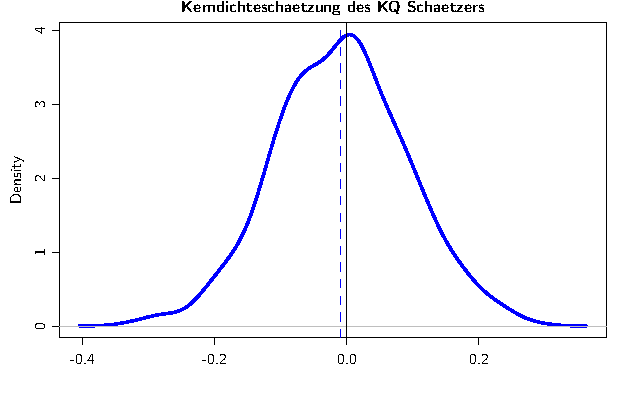
\includegraphics{Resources/Plots/Unbiased2-1} \end{center}
\normalsize
\end{frame}

\begin{frame}{Illustration der bedingten Unverzerrtheit in \R}
\protect\hypertarget{illustration-der-bedingten-unverzerrtheit-in}{}
\xmpl[Simulationsbeispiel]

\begin{itemize}
\tightlist
\item
  Betrachte den DGP \[
  Y_i=\beta_0 + \beta_1 X_i+e_i,\qquad i=1,\ldots,n
  \] mit \(e_i\overset{\text{u.i.v.}}{\sim}N(0,1)\), \(X_i=i\),
  \(\beta_0=0\), \(\beta_1=1\) und \(n=10\).
\item
  (Beispiel: Sie wollen den Einfluss von \alert{Düngermenge} \(X_i\) auf
  \alert{Ertrag} \(Y_i\) des Weizenfeldes messen und legen
  (deterministisch) die Menge \(X_i=i\) für jedes Ihrer 10 Felder fest.)
\item
  Über verschiedene Replikationen \(\{Y_i^{(r)}\}_{i=1,\ldots,n}\)
  (\(r=1,\ldots,\text{reps}\)) hinweg, sollte für den KQ Schätzer
  \(\widehat{\beta}_1^{(r)}\) gelten: \[
  \frac{1}{\text{reps}}\sum_{r=1}^{\text{reps}}\widehat{\beta}_1^{(r)} \approx \E[\widehat{\beta}_1\mid \mX]=\beta_1=1.
  \]
\item
  (Ähnliches gilt natürlich auch für den KQ Schätzer von \(\beta_0\),
  aber wir konzentrieren uns hier auf den Steigungsparameter.)
\end{itemize}

\endxmpl
\end{frame}

\begin{frame}[fragile]{Illustration der bedingten Unverzerrtheit in \R}
\protect\hypertarget{illustration-der-bedingten-unverzerrtheit-in-1}{}
\footnotesize

\begin{Shaded}
\begin{Highlighting}[]
\NormalTok{n    }\OtherTok{\textless{}{-}} \DecValTok{10}              \CommentTok{\# Stichprobenlänge}
\NormalTok{reps }\OtherTok{\textless{}{-}} \DecValTok{500}             \CommentTok{\# Anzahl Wiederholungen}
\NormalTok{X    }\OtherTok{\textless{}{-}} \DecValTok{1}\SpecialCharTok{:}\DecValTok{10}            \CommentTok{\# Fixe Regressoren}
\NormalTok{KQ   }\OtherTok{\textless{}{-}} \FunctionTok{rep}\NormalTok{(}\ConstantTok{NA}\NormalTok{, reps)   }\CommentTok{\# Vektor für KQ Schätzer}

\ControlFlowTok{for}\NormalTok{ (r }\ControlFlowTok{in} \DecValTok{1}\SpecialCharTok{:}\NormalTok{reps)\{}
\NormalTok{   Y     }\OtherTok{\textless{}{-}}\NormalTok{ X }\SpecialCharTok{+} \FunctionTok{rnorm}\NormalTok{(n)    }\CommentTok{\# DGP}
\NormalTok{   KQ[r] }\OtherTok{\textless{}{-}} \FunctionTok{lm}\NormalTok{(Y }\SpecialCharTok{\textasciitilde{}}\NormalTok{ X)}\SpecialCharTok{$}\NormalTok{coefficients[}\DecValTok{2}\NormalTok{]  }\CommentTok{\# Betrachten nur beta\_1 hier}
\NormalTok{\}}
\FunctionTok{plot}\NormalTok{( }\FunctionTok{density}\NormalTok{(KQ), }\AttributeTok{col=}\StringTok{"blue"}\NormalTok{, }\AttributeTok{lwd=}\DecValTok{3}\NormalTok{,}
      \AttributeTok{main=}\StringTok{"Kerndichteschaetzung des KQ Schaetzers gegeben X"}\NormalTok{, }\AttributeTok{xlab=}\StringTok{""}\NormalTok{)}
\FunctionTok{abline}\NormalTok{(}\AttributeTok{v=}\DecValTok{1}\NormalTok{, }\AttributeTok{lty=}\DecValTok{1}\NormalTok{)                     }\CommentTok{\# Wahrer Wert von beta\_1}
\FunctionTok{abline}\NormalTok{(}\AttributeTok{v=}\FunctionTok{mean}\NormalTok{(KQ), }\AttributeTok{lty=}\DecValTok{2}\NormalTok{, }\AttributeTok{col=}\StringTok{"blue"}\NormalTok{)  }\CommentTok{\# Stichprobenmittel über KQ Schätzer}
\end{Highlighting}
\end{Shaded}

\normalsize
\end{frame}

\begin{frame}{Illustration der bedingten Unverzerrtheit in \R}
\protect\hypertarget{illustration-der-bedingten-unverzerrtheit-in-2}{}
\footnotesize
\begin{center}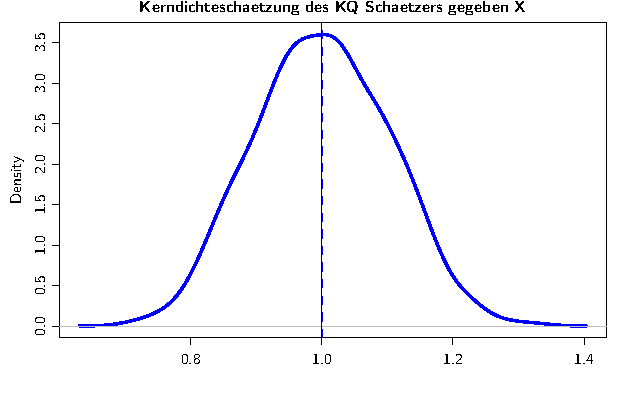
\includegraphics{Resources/Plots/Unbiased4-1} \end{center}
\normalsize
\end{frame}

\begin{frame}{Überblick}
\protect\hypertarget{uxfcberblick-12}{}
\begin{itemize}
\tightlist
\item
  Erwartungswert
\item
  \textbf{Varianz}
\item
  Gauss--Markov Theorem
\item
  Ausschluss und Inklusion von Variablen
\end{itemize}
\end{frame}

\begin{frame}{Varianz-Kovarianz Matrix}
\protect\hypertarget{varianz-kovarianz-matrix}{}
\begin{itemize}
\tightlist
\item
  Erinnern Sie sich an die \hil{Varianz-Kovarianz Matrix} eines
  Zufallsvektors \(\mZ=(Z_1,\ldots,Z_k)^\prime\): \begin{align*}
  \Var(\mZ) & = \E\Big[\big(\mZ-\E[\mZ]\big)\big(\mZ-\E[\mZ]\big)^\prime\Big]\\
          &= \begin{pmatrix}
          \Var(Z_1) & \Cov(Z_1,Z_2) & \ldots & \Cov(Z_1,Z_k)\\
          \Cov(Z_2,Z_1) & \Var(Z_2) & \ldots & \Cov(Z_2,Z_k)\\
          \vdots        & \vdots    &  \ddots&  \vdots      \\
          \Cov(Z_k,Z_1) & \Cov(Z_k,Z_2)& \ldots & \Var(Z_k)
          \end{pmatrix}.
  \end{align*}
\item
  Analog dazu definieren wir die \hil{bedingte Varianz-Kovarianz Matrix}
  von \(\mZ\) gegeben \(\mX\): \begin{equation}\label{eq:bed Var}
  \Var(\mZ\mid \mX) = \E\Big[\big(\mZ-\E[\mZ\mid \mX]\big)\big(\mZ-\E[\mZ\mid \mX]\big)^\prime\mid \mX\Big].
  \end{equation}
\item
  Aus Definition folgt direkt (gilt auch bedingt):
  \begin{equation}\label{eq:Form VaR}
  \Var(\mA^\prime \mZ)=\mA^\prime\Var( \mZ)\mA.
  \end{equation}
\end{itemize}
\end{frame}

\begin{frame}{Varianz}
\protect\hypertarget{varianz}{}
\begin{itemize}
\tightlist
\item
  Um die Varianz des KQ Schätzers herzuleiten, ist folgende Formel
  hilfreich: \begin{eqnarray}
  \widehat{\vbeta} & \overset{\eqref{eq:beta hat mat}}{=} & (\mX^\prime\mX)^{-1}\mX^\prime\mY\notag\\
   & \overset{\eqref{eq:lbE}}{=} & (\mX^\prime\mX)^{-1}\mX^\prime(\mX\vbeta + \ve)\notag\\
   &=& \vbeta + (\mX^\prime\mX)^{-1}\mX^\prime\ve.\label{eq:decomp beta hat}
  \end{eqnarray}
\item
  Für
  \(\mD:=\Var(\ve\mid\mX)\overset{\eqref{eq:bed Var}}{\underset{\E[\ve\mid\mX]=\vzero}{=}}\E[\ve\ve^\prime\mid \mX]\)
  gilt:

  \begin{itemize}
  \tightlist
  \item
    Das \(i\)-te Diagonalelement ist \[
    \E[e_i^2\mid \mX] \overset{\text{ÜA}}{=} \E[e_i^2\mid X_i]=:\sigma_i^2.
    \]
  \item
    Das \((i,j)\)-te Element ist (ÜA über Dichten) \[
    \E[e_i e_j\mid \mX] = \E[e_i\mid X_i]\E[e_j\mid X_j] = 0.
    \]
  \end{itemize}
\item
  Damit: \(\mD=\diag(\sigma_1^2,\ldots,\sigma_n^2)\).
\end{itemize}
\end{frame}

\begin{frame}{Varianz}
\protect\hypertarget{varianz-1}{}
\begin{itemize}
\item
  Aus der Definition der Varianz-Kovarianz Matrix folgt unmittelbar
  \begin{eqnarray}
  \Var(\widehat{\vbeta}\mid \mX) &\overset{\eqref{eq:decomp beta hat}}{=} &\Var(\vbeta + (\mX^\prime\mX)^{-1}\mX^\prime\ve\mid \mX)\notag\\
  &=&\Var((\mX^\prime\mX)^{-1}\mX^\prime\ve\mid \mX)\notag\\
  &\overset{\eqref{eq:Form VaR}}{=}& (\mX^\prime\mX)^{-1}\mX^\prime\Var(\ve\mid \mX)\mX(\mX^\prime\mX)^{-1}\notag\\
  &=& (\mX^\prime\mX)^{-1}\mX^\prime\mD\mX(\mX^\prime\mX)^{-1}.\label{eq:var form ols}
  \end{eqnarray}
\item
  Die obige Formel für \(\Var(\widehat{\vbeta}\mid \mX)\) ist sehr lang.
\item
  Unter \alert{Homoskedastie} vereinfacht sie sich aber
  erheblich\ldots{}
\end{itemize}
\end{frame}

\begin{frame}{Varianz}
\protect\hypertarget{varianz-2}{}
\framesubtitle{Homoskedastie}

\ass[Bedingte Homoskedastie]\label{ass:cond hom} Die Fehler sind
\hil{bedingt homoskedastisch}, d.h. \[
  \E[e^2\mid X]=\sigma^2.
\] Gilt dies nicht, so sind die Fehler \hil{bedingt heteroskedastisch}.
\endass

\begin{itemize}
\tightlist
\item
  Unter \alert{bedingter Homoskedastie} gilt wegen Verschiebungssatz
  \begin{eqnarray}
  \var(e\mid X) &=& \E[e^2\mid X] - \big(\E[e\mid X]\big)^2\notag\\
  &\overset{\eqref{eq:lbE}}{=}&  \E[e^2\mid X]\notag \\
  &=& \sigma^2\notag\\
  \Rightarrow\ \mD=\Var(\ve\mid \mX) & = & \sigma^2\mI.\label{eq:homo impl}
  \end{eqnarray}
\item
  Dies einsetzen in \eqref{eq:var form ols} liefert: \[
  \Var(\widehat{\vbeta}\mid \mX) = \sigma^2(\mX^\prime\mX)^{-1}.
  \]
\end{itemize}
\end{frame}

\begin{frame}{Varianz}
\protect\hypertarget{varianz-3}{}
\framesubtitle{Homoskedastie}

\begin{itemize}
\tightlist
\item
  \emph{In praxi} gilt Homoskedastie sehr selten, aber die Formel ist
  nützlich, um die \alert{Intuition} für die Formel zu schärfen.
\item
  Die Varianz
  \(\Var(\widehat{\vbeta}\mid \mX) = \sigma^2(\mX^\prime\mX)^{-1}\) ist
  \alert{größer}, \ldots{}

  \begin{itemize}
  \tightlist
  \item
    \ldots{} je \alert{größer} die Fehlervarianz
    \(\sigma^2=\Var(e\mid X)\) und
  \item
    \ldots{} je \alert{kleiner} die Schwankungsbreite der \(X\) und
  \item
    \ldots{} je \alert{kleiner} \(n\).
  \end{itemize}
\item
  Beachte für die letzten beiden Punkte mit \(X_i=(1,X_{1i})^\prime\),
  dass \begin{align*}
   (\mX^\prime\mX)^{-1}&=\bigg(\sum_{i=1}^{n}X_iX_i^\prime\bigg)^{-1}=\left(\begin{pmatrix}n & \sum_{i=1}^{n}X_{1i}\\ \sum_{i=1}^{n}X_{1i} & \sum_{i=1}^{n}X_{1i}^2\end{pmatrix}\right)^{-1}\\
   &= \frac{1}{n\sum_{i=1}^{n}X_{1i}^2 - \big(\sum_{i=1}^{n}X_{1i}\big)^2}\begin{pmatrix} \sum_{i=1}^{n}X_{1i}^2 & -\sum_{i=1}^{n}X_{1i}\\ -\sum_{i=1}^{n}X_{1i} & n\end{pmatrix}\\
   &= \underbrace{\frac{1}{n}}_{=Stichprobe}\underbrace{\frac{1}{\frac{1}{n}\sum_{i=1}^{n}X_{1i}^2 - \big(\frac{1}{n}\sum_{i=1}^{n}X_{1i}\big)^2}}_{=Stichprobenvarianz=Schwankungsbreite}\begin{pmatrix} \frac{1}{n}\sum_{i=1}^{n}X_{1i}^2 & -\frac{1}{n}\sum_{i=1}^{n}X_{1i}\\ -\frac{1}{n}\sum_{i=1}^{n}X_{1i} & 1\end{pmatrix}.
  \end{align*}
\end{itemize}
\end{frame}

\begin{frame}{Varianz}
\protect\hypertarget{varianz-4}{}
\begin{itemize}
\tightlist
\item
  Wir sammeln die Resultate im folgenden
\end{itemize}

\thmn[Hansen (2022, Theorem 4.2)]\label{thm:Var KQ} Im linearen
bedingten Erwartungswertmodell \eqref{eq:lbE} gilt unter den Annahmen
\ref{ass:1}, \ref{ass:iid} und \ref{ass:pd}, dass \[
  \Var(\widehat{\vbeta}\mid \mX)=(\mX^\prime\mX)^{-1}\mX^\prime\mD\mX(\mX^\prime\mX)^{-1}.
\] Unter der zusätzlichen Annahme \ref{ass:cond hom} vereinfacht sich
die Formel zu \[
  \Var(\widehat{\vbeta}\mid \mX) = \sigma^2(\mX^\prime\mX)^{-1}.
\] \endthmn

\begin{itemize}
\tightlist
\item
  Beachte: Homoskedastie (Annahme \ref{ass:cond hom}) beschreibt
  Zusammenhang von \((X_i,e_i=Y_i-X_i^\prime\vbeta)\) \alert{innerhalb}
  einer Beobachtung, \ldots{}
\item
  \ldots{} während u.i.v. (Annahme \ref{ass:iid}) den Zusammenhang
  \alert{zwischen} \((X_i, Y_i)\) und \((X_j, Y_j)\) (\(i\neq j\))
  beschreibt.
\end{itemize}
\end{frame}

\begin{frame}{Illustration von Heteroskedastie in \R}
\protect\hypertarget{illustration-von-heteroskedastie-in}{}
\xmpl[Card (1995)]

\begin{itemize}
\tightlist
\item
  Erinnern Sie sich an die Lohnregression von Card (1995) aus
  Beispiel~\ref{ex:Card}: \[
   \log(wage) = \beta_0+\beta_1\cdot educ + e.
   \]
\item
  Die Fehler in diesem Modell sind \alert{bedingt heteroskedastisch}, da
  je länger die Ausbildungsdauer, desto größer die Varianz im Verdienst
  (d.h. \(\Var(e\mid X)\) steigt in \(X\)).
\end{itemize}

\footnotesize
\begin{center}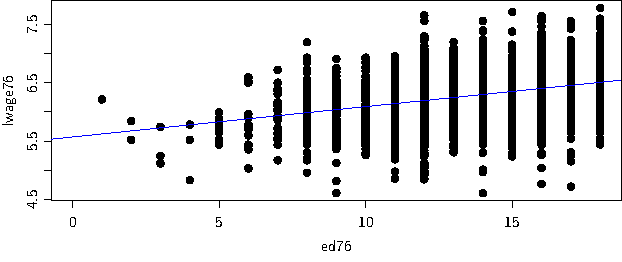
\includegraphics{Resources/Plots/Heterosk-1} \end{center}
\normalsize

\endxmpl
\end{frame}

\begin{frame}{Unbedingte Varianz}
\protect\hypertarget{unbedingte-varianz}{}
\begin{itemize}
\tightlist
\item
  Ähnlich wie schon beim Erwartungswert können wir auch hier von der
  \alert{bedingten} Varianz aus Theorem \ref{thm:Var KQ} auf die
  \alert{unbedingte} Varianz schließen.
\end{itemize}

\thmn[Hansen (2022, Theorem 2.8)]\label{thm:Var decomp} Wenn
\(\E[Y^2]<\infty\), dann gilt
\(\Var(Y)=\E\big[\Var(Y\mid X)\big] + \Var\big(\E[Y\mid X]\big)\).
\endthmn

\begin{itemize}
\tightlist
\item
  Unbedingte Varianz zerlegt sich in

  \begin{itemize}
  \tightlist
  \item
    ersten Term (\alert{"within group variance"}): Erwartete Varianz von
    \(Y\) innerhalb Gruppe \(X\);
  \item
    zweiten Term (\alert{"across group variance"}): Varianz von
    erwartetem \(Y\) zwischen Gruppen \(X\).
  \end{itemize}
\item
  Falls \(\E[\widehat{\vbeta}^2]<\infty\), \begin{eqnarray*}
  \Var(\widehat{\vbeta}) &\overset{\text{Thm.}\ \ref{thm:Var decomp}}{=} & \E\big[\Var(\widehat{\vbeta}\mid \mX)\big] + \Var\big(\E[\widehat{\vbeta}\mid \mX]\big) \\
  &\overset{\text{Thm.}\ \ref{thm:cond exp ols}}{=}& \E\big[\Var(\widehat{\vbeta}\mid \mX)\big] + \underbrace{\Var\big(\vbeta\big)}_{=\vzero} \\
  &\overset{\text{Thm.}\ \ref{thm:Var KQ}}{=} & \E\big[(\mX^\prime\mX)^{-1}\mX^\prime\mD\mX(\mX^\prime\mX)^{-1}\big].
  \end{eqnarray*}
\end{itemize}
\end{frame}

\begin{frame}{Überblick}
\protect\hypertarget{uxfcberblick-13}{}
\begin{itemize}
\tightlist
\item
  Erwartungswert
\item
  Varianz
\item
  \textbf{Gauss--Markov Theorem}
\item
  Ausschluss und Inklusion von Variablen
\end{itemize}
\end{frame}

\begin{frame}{Motivation}
\protect\hypertarget{motivation}{}
\begin{itemize}
\tightlist
\item
  KQ ist unverzerrt,
  d.h.~\(\E\big[\widehat{\vbeta}\mid\mX\big]=\vbeta\), aber das gilt für
  \alert{andere Schätzer} auch.

  \begin{itemize}
  \tightlist
  \item
    Z.B.~gilt für
    \(\widetilde{\vbeta}=(\mZ^\prime\mX)^{-1}\mZ^\prime\mY\) mit
    \(Z_i=X_i^2\) auch, dass
    \(\E\big[\widetilde{\vbeta}\mid\mX\big]=\vbeta\).
  \end{itemize}
\item
  Wir können nicht sagen, dass KQ besser als diese ist -- sie sind alle
  \alert{gleich} unverzerrt!
\item
  \alert{Frage:} Warum sollten wir also unbedingt den KQ Schätzer
  benutzen?
\item
  \alert{Antwort:} Weil er vielleicht niedrigere Varianz besitzt, also
  weniger um den wahren Wert herum streut.
\end{itemize}

\defn

Ein Schätzer \(\overline{\vbeta}\) hat \hil{niedrigere Varianz} als
\(\widetilde{\vbeta}\), wenn
\(\Var(\widetilde{\vbeta})-\Var(\overline{\vbeta})\) positiv
semi-definit (p.s.d.) ist (geschrieben:
\(\Var(\widetilde{\vbeta})-\Var(\overline{\vbeta})\geq0\) oder auch
\(\Var(\widetilde{\vbeta})\geq\Var(\overline{\vbeta})\)). \enddefn

\begin{itemize}
\tightlist
\item
  \alert{Warum?} Weil so \emph{jede} Linearkombination
  \(\vc^\prime\overline{\vbeta}\) nicht größere Varianz hat als dieselbe
  Linearkombination \(\vc^\prime\widetilde{\vbeta}\), d.h. \[
  \Var(\vc^\prime\widetilde{\vbeta})-\Var(\vc^\prime\overline{\vbeta})\overset{\eqref{eq:Form VaR}}{=}\vc^\prime\big[\Var(\widetilde{\vbeta})-\Var(\overline{\vbeta})\big]\vc\geq0.
  \]
\end{itemize}
\end{frame}

\begin{frame}{Gauss--Markov Theorem}
\protect\hypertarget{gaussmarkov-theorem}{}
\begin{itemize}
\tightlist
\item
  Das \hil{Gauss--Markov Theorem (GMT)} betrachtet

  \begin{enumerate}
  \tightlist
  \item
    \alert{lineare Schätzer:} \(\widetilde{\vbeta}=\mA^\prime\mY\) mit
    \(\mA=\mA(\mX)\) eine \((k\times n)\)-Matrix;
  \item
    \alert{unverzerrte Schätzer:}
    \(\E\big[\widetilde{\vbeta}\mid \mX\big]=\vbeta\).
  \end{enumerate}
\item
  Das GMT besagt, dass KQ in einer wichtigen Klasse von Schätzern (den
  linearen und unverzerrten) die \alert{niedrigste Varianz} besitzt --
  KQ ist der \hil{best linear unbiased estimator (BLUE)}!
\end{itemize}

\thmn[Gauss--Markov Theorem]\label{thm:GMT} Betrachte das lineare
bedingte Erwartungswertmodell \eqref{eq:lbE}. Sei \(\widetilde{\vbeta}\)
ein \alert{linearer} und \alert{unverzerrter} Schätzer. Dann gilt unter
den Annahmen \ref{ass:1}, \ref{ass:iid}, \ref{ass:pd} und
\ref{ass:cond hom}, dass \[
  \Var(\widetilde{\vbeta}\mid\mX)\geq\sigma^2(\mX^\prime\mX)^{-1}=\Var(\widehat{\vbeta}\mid \mX).
\] \endthmn
\end{frame}

\begin{frame}{Beweis}
\protect\hypertarget{beweis}{}
\begin{block}{Beweis von Theorem \ref{thm:GMT} (1/2)}
Aus $\widetilde{\vbeta}=\mA^\prime\mY$ folgt
\[
  \E\big[\widetilde{\vbeta}\mid\mX\big] \overset{\eqref{eq:pull out}}{=} \mA^\prime\E[\mY\mid\mX]\overset{\eqref{eq:lbE}}{=}\mA^\prime\mX\vbeta.
\]
Da $\widetilde{\vbeta}$ unverzerrt ist, muss gelten $\mA^\prime\mX=\mI_k$.\medskip

Des Weiteren gilt unter Annahme \ref{ass:cond hom},
\begin{eqnarray*}
  \Var(\widetilde{\vbeta}\mid \mX) &=& \Var(\mA^\prime\mY\mid\mX)\\
  &\overset{\eqref{eq:Form VaR}}{=} & \mA^\prime\Var(\mY\mid\mX)\mA\\
  &\overset{\eqref{eq:lbE}}{=} & \mA^\prime\Var(\mX\vbeta+\ve\mid\mX)\mA\\
  &=& \mA^\prime\Var(\ve\mid\mX)\mA\\
  &\overset{\eqref{eq:homo impl}}{=}&\sigma^2\mA^\prime\mA.
\end{eqnarray*}

Wir müssen also nur noch zeigen, dass für alle $\mA$ mit $\mA^\prime\mX=\mI_{k}$ gilt, dass
\[
  \mA^\prime\mA\geq(\mX^\prime\mX)^{-1}.
\]
\end{block}
\end{frame}

\begin{frame}{Beweis}
\protect\hypertarget{beweis-1}{}
\begin{block}{Beweis von Theorem \ref{thm:GMT} (2/2)}
Setze $\mC=\mA-\mX(\mX^\prime\mX)^{-1}$. Wegen $\mA^\prime\mX=\mI_{k}$ gilt $\mX^\prime\mC=\vzero$. Damit:
\begin{align*}
  \mA^\prime\mA - (\mX^\prime\mX)^{-1} &= \big(\mC + \mX(\mX^\prime\mX)^{-1}\big)^\prime \big(\mC + \mX(\mX^\prime\mX)^{-1}\big) - (\mX^\prime\mX)^{-1}\\
  &= \mC^\prime\mC + \underbrace{\mC^\prime\mX}_{=(\mX^\prime\mC)^\prime=\vzero}(\mX^\prime\mX)^{-1} + (\mX^\prime\mX)^{-1}\underbrace{\mX^\prime\mC}_{=\vzero}\\
  &\hspace{1cm} + \underbrace{(\mX^\prime\mX)^{-1}\mX^\prime\mX}_{=\mI_k}(\mX^\prime\mX)^{-1} - (\mX^\prime\mX)^{-1}\\
  &= \mC^\prime\mC\geq0.
\end{align*}
Beachte für letzte Ungleichung: Klar, dass $\mC^\prime\mC$ p.s.d., da für alle Vektoren $\vx$,
\[
  \vx^\prime\mC^\prime\mC\vx=(\mC\vx)^\prime(\mC\vx)\geq0.
\]
\end{block}
\end{frame}

\begin{frame}{Illustration des GMT via \R Beispiel}
\protect\hypertarget{illustration-des-gmt-via-beispiel}{}
\xmpl[Simulationsbeispiel]

\begin{itemize}
\tightlist
\item
  Betrachte wieder den DGP \[
  Y_i=\beta_0+e_i,\qquad i=1,\ldots,n
  \] mit \(\beta_0=0\) und \(e_i\overset{\text{u.i.v.}}{\sim}N(0,1)\).
\item
  Der KQ Schätzer ist
  \(\widehat{\beta}_0=\frac{1}{n}\sum_{i=1}^{n}Y_i\).
\item
  Der zweite Schätzer, den wir betrachten, ist der
  \alert{gewichtete Schätzer} \[
  \widetilde{\beta}_0=\sum_{i=1}^{n}w_i Y_i,\qquad w_i=\begin{cases} \frac{1.5}{n},& i=1,\ldots,n/2;\\
  \frac{0.5}{n}, & i=n/2+1,\ldots,n.\end{cases}
  \]

  \begin{itemize}
  \tightlist
  \item
    \alert{linear:} Klar!
  \item
    \alert{unverzerrt:} Auch klar, wegen Wahl der Gewichte.
  \end{itemize}
\item
  Nach dem GMT müsste \(\widetilde{\beta}_0\) also breiter streuen als
  \(\widehat{\beta}_0\)!
\end{itemize}

\endxmpl
\end{frame}

\begin{frame}[fragile,allowframebreaks]{Illustration des GMT via
\R Beispiel}
\protect\hypertarget{illustration-des-gmt-via-beispiel-1}{}
\footnotesize

\begin{Shaded}
\begin{Highlighting}[]
\NormalTok{n    }\OtherTok{\textless{}{-}} \DecValTok{100}      
\NormalTok{reps }\OtherTok{\textless{}{-}} \FloatTok{1e6}

\NormalTok{epsilon }\OtherTok{\textless{}{-}} \FloatTok{0.5}
\NormalTok{w       }\OtherTok{\textless{}{-}} \FunctionTok{c}\NormalTok{(}\FunctionTok{rep}\NormalTok{((}\DecValTok{1}\SpecialCharTok{+}\NormalTok{epsilon)}\SpecialCharTok{/}\NormalTok{n,n}\SpecialCharTok{/}\DecValTok{2}\NormalTok{), }\FunctionTok{rep}\NormalTok{((}\DecValTok{1}\SpecialCharTok{{-}}\NormalTok{epsilon)}\SpecialCharTok{/}\NormalTok{n,n}\SpecialCharTok{/}\DecValTok{2}\NormalTok{))}

\NormalTok{ols }\OtherTok{\textless{}{-}}\NormalTok{ weightedestimator }\OtherTok{\textless{}{-}} \FunctionTok{rep}\NormalTok{(}\ConstantTok{NA}\NormalTok{, reps)}

\ControlFlowTok{for}\NormalTok{ (i }\ControlFlowTok{in} \DecValTok{1}\SpecialCharTok{:}\NormalTok{reps)\{}
\NormalTok{  y                    }\OtherTok{\textless{}{-}} \FunctionTok{rnorm}\NormalTok{(n)}
\NormalTok{  ols[i]               }\OtherTok{\textless{}{-}} \FunctionTok{mean}\NormalTok{(y)}
\NormalTok{  weightedestimator[i] }\OtherTok{\textless{}{-}} \FunctionTok{crossprod}\NormalTok{(w,y)  }
\NormalTok{\}}

\FunctionTok{plot}\NormalTok{( }\FunctionTok{density}\NormalTok{(ols), }\AttributeTok{col=}\StringTok{"blue"}\NormalTok{, }\AttributeTok{lwd=}\DecValTok{3}\NormalTok{, }
     \AttributeTok{main=}\StringTok{"Kerndichteschaetzung des KQ und gewichteten Schaetzers"}\NormalTok{, }\AttributeTok{xlab=}\StringTok{""}\NormalTok{)}
\FunctionTok{lines}\NormalTok{( }\FunctionTok{density}\NormalTok{(weightedestimator), }\AttributeTok{col=}\StringTok{"red"}\NormalTok{, }\AttributeTok{lwd=}\DecValTok{3}\NormalTok{)     }

\FunctionTok{abline}\NormalTok{(}\AttributeTok{v=}\DecValTok{0}\NormalTok{, }\AttributeTok{lty=}\DecValTok{2}\NormalTok{)}
\FunctionTok{legend}\NormalTok{(}\StringTok{\textquotesingle{}topright\textquotesingle{}}\NormalTok{, }\FunctionTok{c}\NormalTok{(}\StringTok{"$}\SpecialCharTok{\textbackslash{}\textbackslash{}}\StringTok{widehat\{}\SpecialCharTok{\textbackslash{}\textbackslash{}}\StringTok{beta\}\_0$"}\NormalTok{, }\StringTok{"$}\SpecialCharTok{\textbackslash{}\textbackslash{}}\StringTok{widetilde\{}\SpecialCharTok{\textbackslash{}\textbackslash{}}\StringTok{beta\}\_0$"}\NormalTok{), }
                                                            \AttributeTok{col=}\FunctionTok{c}\NormalTok{(}\StringTok{"blue"}\NormalTok{, }\StringTok{"red"}\NormalTok{), }\AttributeTok{lwd=}\DecValTok{3}\NormalTok{)}
\end{Highlighting}
\end{Shaded}

\begin{center}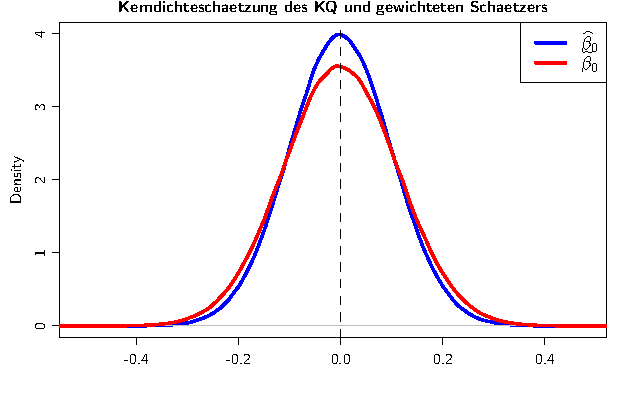
\includegraphics{Resources/Plots/GMT-1} \end{center}
\normalsize
\end{frame}

\begin{frame}{Überblick}
\protect\hypertarget{uxfcberblick-14}{}
\begin{itemize}
\tightlist
\item
  Erwartungswert
\item
  Varianz
\item
  Gauss--Markov Theorem
\item
  \textbf{Ausschluss und Inklusion von Variablen}
\end{itemize}
\end{frame}

\begin{frame}{Ausschluss relevanter Variablen}
\protect\hypertarget{ausschluss-relevanter-variablen}{}
\begin{itemize}
\tightlist
\item
  Wir interessieren uns für \(\vbeta_1\) im
  \alert{partitionierten wahren DGP} \begin{equation}\label{eq:true DGP}
  \mY=\mX_1\vbeta_1 + \mX_2\vbeta_2+\vu,\qquad\E[\vu\mid\mX]=\vzero.
  \end{equation}

  \begin{itemize}
  \tightlist
  \item
    \alert{Erinnerung:} In linearen Modellen reicht anstatt der BUA
    schon \(\E[\vu\mid\mX]=\vzero\).
  \end{itemize}
\item
  Wir führen jedoch die Schätzung basierend auf folgendem Modell durch:
  \begin{equation}\label{eq:small model}
  \mY=\mX_1\vbeta + \ve,\qquad\E[\mX^\prime\ve]=\vzero.
  \end{equation}

  \begin{itemize}
  \tightlist
  \item
    Dies ist nicht mehr der wahre DGP, sondern nur noch zu
    interpretieren als \alert{lineares Projektionsmodell} -- deshalb
    \(\ve\) anstatt \(\vu\).
  \end{itemize}
\item
  Wir lassen also \alert{relevante Variablen} aus (wenn
  \(\vbeta_2\neq\vzero\)) und schätzen den Einfluss von \(\mX_1\) auf
  \(\mY\) via \[
  \widehat{\vbeta}=(\mX_1^\prime\mX_1)^{-1}\mX_1^\prime\mY.
  \]
\end{itemize}
\end{frame}

\begin{frame}{Ausschluss relevanter Variablen}
\protect\hypertarget{ausschluss-relevanter-variablen-1}{}
\begin{itemize}
\tightlist
\item
  Die Konsequenz dieses Auslassens ist eine \alert{verzerrte Schätzung}
  des kausalen Effekts \(\vbeta_1\): \begin{eqnarray*}
  \E\big[\widehat{\vbeta}\mid\mX\big] &\overset{\eqref{eq:pull out}}{=} & (\mX_1^\prime\mX_1)^{-1}\mX_1^\prime\E[\mY\mid\mX]\\
  & \overset{\eqref{eq:true DGP}}{=} & (\mX_1^\prime\mX_1)^{-1}\mX_1^\prime\E[\mX_1\vbeta_1 + \mX_2\vbeta_2+\vu\mid\mX] \\
  &\overset{\eqref{eq:pull out}}{=}& (\mX_1^\prime\mX_1)^{-1}\mX_1^\prime(\mX_1\vbeta_1 + \mX_2\vbeta_2)\\
  &=& \vbeta_1 + (\mX_1^\prime\mX_1)^{-1}\mX_1^\prime\mX_2\vbeta_2.
  \end{eqnarray*}
\item
  Dies ist \alert{ungleich} \(\vbeta_1\), außer wenn

  \begin{enumerate}
  \tightlist
  \item
    \(\vbeta_2=\vzero\) (also wenn die zusätzlichen Regressoren
    irrelevant sind) \alert{oder}
  \item
    \(\mX_1^\prime\mX_2=\vzero\) (also wenn \(\mX_1\) und \(\mX_2\)
    orthogonal).
  \end{enumerate}
\item
  Also gilt i.A.: Ausschluss relevanter Variablen führt zu verzerrter
  Schätzung.
\end{itemize}
\end{frame}

\begin{frame}{Inklusion irrelevanter Variablen}
\protect\hypertarget{inklusion-irrelevanter-variablen}{}
\begin{itemize}
\tightlist
\item
  Nehme jetzt an, dass \eqref{eq:small model} das wahre Modell ist (mit
  dann \(\ve=\vu\) und \(\E[\vu\mid\mX_1]=\vzero\) sowie
  \(\vbeta_1=\vbeta\)), \ldots{}
\item
  \ldots{} wir jedoch auf Basis von Modell \eqref{eq:true DGP} schätzen.
\item
  Dies bedeutet \alert{Inklusion irrelevanter Variablen}, da
  \(\vbeta_2=\vzero\).
\item
  Beide Modelle \eqref{eq:true DGP} und \eqref{eq:small model} sind also
  korrekt, jedoch verwendet \eqref{eq:small model} die Information, dass
  \(\vbeta_2=\vzero\), \eqref{eq:true DGP} jedoch nicht.
\end{itemize}
\end{frame}

\begin{frame}{Inklusion irrelevanter Variablen}
\protect\hypertarget{inklusion-irrelevanter-variablen-1}{}
\begin{itemize}
\tightlist
\item
  Der Schätzer basierend auf der \hil{langen Regression}
  \eqref{eq:true DGP} \[
  \widehat{\vbeta}_1\overset{\eqref{eq:(2.15)}}{=} (\mX_1^\prime\mM_{\mX_2}\mX_1)^{-1}\mX_1^\prime\mM_{\mX_2}\mY
  \] ist offensichtlich \alert{linear} und auch \alert{unverzerrt}, da
  \(\E\big[\widehat{\vbeta}_1\mid\mX_1\big] \overset{\eqref{eq:GIE advanced}}{=} \E\Big(\E\big[\widehat{\vbeta}_1 \mid\mX_1,\mX_2\big]\mid\mX_1\Big)\)
  und \begin{eqnarray*}
  \E\big[\widehat{\vbeta}_1\mid\mX_1,\mX_2\big] &=&\E\big[(\mX_1^\prime\mM_{\mX_2}\mX_1)^{-1}\mX_1^\prime\mM_{\mX_2}\mY\mid\mX\big]\\
  &\overset{\eqref{eq:pull out}}{=}& (\mX_1^\prime\mM_{\mX_2}\mX_1)^{-1}\mX_1^\prime\mM_{\mX_2}\E\big[\mY\mid\mX\big]\\
  &\overset{\eqref{eq:small model}}{=}&  (\mX_1^\prime\mM_{\mX_2}\mX_1)^{-1}\mX_1^\prime\mM_{\mX_2}\E\big[\mX_1\vbeta+\vu\mid\mX\big]\\
  &\overset{\eqref{eq:pull out}}{=}&  (\mX_1^\prime\mM_{\mX_2}\mX_1)^{-1}\mX_1^\prime\mM_{\mX_2}\big(\mX_1\vbeta+\underbrace{\E[\vu\mid\mX]}_{=\vzero}\big)=\vbeta\\
   \Longrightarrow\quad \E\big[\widehat{\vbeta}_1\mid\mX_1\big] &=& \vbeta.
  \end{eqnarray*}
\item
  Nach GMT gilt also:
  \(\Var(\widehat{\vbeta}_1\mid\mX_1)\geq \Var(\widehat{\vbeta}\mid\mX_1)\).
\end{itemize}
\end{frame}

\begin{frame}{Zusammenfassung}
\protect\hypertarget{zusammenfassung}{}
\begin{itemize}
\tightlist
\item
  \alert{Zusätzliche} Regressoren reduzieren das Risiko der
  \hil{Verzerrung durch ausgelassene Variablen}, was (sehr) gut ist.
\item
  Auf der anderen Seite verringern sie die
  \alert{Präzision des Schätzers}, was weniger gut ist.
\item
  Bei \alert{großem $n$:} \emph{Über}spezifizierung naheliegend, da
  Verzerrung durch Unterspezifizierung nicht mit \(n\) verschwindet,
  aber dank großem \(n\) der Schätzer immer noch recht präzise ist.
\item
  Bei \alert{kleinem $n$:} \emph{Unter}spezifizierung naheliegend, da
  Hinzunahme von zu vielen Variablen zu Effizienzverlusten führen kann,
  die schwerer wiegen als Verzerrung durch ausgelassene Variablen.
\end{itemize}
\end{frame}

\hypertarget{eigenschaften-von-kq-in-grouxdfen-stichproben}{%
\section{Eigenschaften von KQ in großen
Stichproben}\label{eigenschaften-von-kq-in-grouxdfen-stichproben}}

\begin{frame}{}
\protect\hypertarget{section-4}{}
\centerline{\textbf{Eigenschaften von KQ in großen Stichproben}}
\centerline{(Hansen, 2022, Kapitel 7)}
\end{frame}

\begin{frame}{Ausblick}
\protect\hypertarget{ausblick}{}
\begin{itemize}
\tightlist
\item
  Im vorherigen Kapitel: Können Erwartungswert und Varianz des KQ
  Schätzers \alert{für jedes $n$} bestimmen.
\item
  Aber: Über die \alert{Verteilung} von \(\widehat{\vbeta}\) für fixes
  \(n\) können wir ohne weitere Annahmen nichts aussagen.

  \begin{itemize}
  \tightlist
  \item
    Mit \alert{normalverteilten Fehlern} ginge es (siehe Hansen, 2022,
    Kapitel 5), aber wir verfolgen das nicht weiter.
  \end{itemize}
\item
  Also: Brauchen \alert{Asymptotik}, d.h.~\(n\to\infty\).
\item
  Dazu wiederholen wir zunächst einige Grundbegriffe.
\item
  Danach untersuchen wir \(\widehat{\vbeta}\) in unserem (allgemeinsten)
  \alert{linearen Projektionsmodell}.
\end{itemize}
\end{frame}

\begin{frame}{Überblick}
\protect\hypertarget{uxfcberblick-15}{}
\begin{itemize}
\tightlist
\item
  \textbf{Wiederholung asymptotischer Theorie}
\item
  Konsistenz des KQ Schätzers
\item
  Asymptotische Normalität des KQ Schätzers
\end{itemize}
\end{frame}

\begin{frame}{Wiederholung asymptotischer Theorie}
\protect\hypertarget{wiederholung-asymptotischer-theorie}{}
\begin{itemize}
\tightlist
\item
  In \(\widehat{\vbeta}\) aus \eqref{eq:beta hat mat} taucht eine
  \alert{Zufallsmatrix} \((\mX^\prime\mX)\) auf.
\item
  Wir werden hier bekannte Konvergenzbegriffe wiederholen und dabei (wo
  nötig) \alert{auf Zufallsmatrizen erweitern}.
\item
  Konvergenz benötigt immer einen \alert{Abstandsbegriff}, also -- in
  mathematischer Sprache -- eine \alert{Norm}.
\item
  Dazu führen wir für \((k\times\ell)\)-Matrizen
  \(\mA=(A_{ij})_{\substack{i=1,\ldots,k\\ j=1,\ldots,\ell}}\) die
  \hil{euklidische Norm} ein: \[
  \boxed{ \Vert \mA \Vert := \sqrt{\sum_{i=1}^{k}\sum_{j=1}^{\ell} A_{ij}^2}. }
  \]
\item
  Wenn \(\mA=(A_1,\ldots, A_k)^\prime\) ein \alert{Vektor} ist (also
  eine \((k\times 1)\)-Matrix), wird unmittelbar klar, woher der Name
  kommt, denn: \[
  \Vert \mA \Vert = \sqrt{A_1^2+\ldots+A_k^2}.
  \]
\item
  Wenn \(A\) ein \alert{Skalar} ist (also eine \((1\times 1)\)-Matrix),
  wird die euklidische Norm zum \hil{Absolutbetrag} \[
  \Vert A \Vert = |A|.
  \]
\end{itemize}
\end{frame}

\begin{frame}{Konvergenzmodi}
\protect\hypertarget{konvergenzmodi}{}
\framesubtitle{Definitionen}

\defn[Konvergenz in Wahrscheinlichkeit]Die Zufallsmatrizen \(\mZ_n\)
\hil{konvergieren in Wahrscheinlichkeit} gegen (\alert{zufälliges} oder
\alert{deterministisches}) \(\mZ\) (geschrieben:
\(\mZ_n\overset{\Pr}{\longrightarrow}\mZ\)), wenn für alle
\(\epsilon>0\) \[
  \lim_{n\to\infty}\Pr\big\{\Vert \mZ_n-\mZ\Vert\leq\epsilon\big\}=1.
\] \enddefn

\defn[Konvergenz in Verteilung]Die Zufallsvektoren \(\mZ_n\)
\hil{konvergieren in Verteilung} gegen \(\mZ\) (geschrieben:
\(\mZ_n\overset{d}{\longrightarrow}\mZ\)), wenn \[
  F_{\mZ_n}(\vz)\underset{(n\to\infty)}{\longrightarrow} F_{\mZ}(\vz)
\] für alle Stetigkeitsstellen \(\vz\) von \(F_{\mZ}(\cdot)\). \(\mZ\)
heißt \hil{asymptotische Verteilung} von \(\mZ_n\). \enddefn

\begin{itemize}
\tightlist
\item
  Konvergenz in \alert{Wahrscheinlichkeit:} \(\mZ_n\) und \(\mZ\) werden
  sich ähnlicher.
\item
  Konvergenz in \alert{Verteilung:} \emph{Verteilungsfunktionen} von
  \(\mZ_n\) und \(\mZ\) werden sich ähnlicher.
\end{itemize}
\end{frame}

\begin{frame}{Konvergenzmodi}
\protect\hypertarget{konvergenzmodi-1}{}
\framesubtitle{Beispiele}

\xmpl

\begin{itemize}
\tightlist
\item
  Sei \(Z\sim N(0,1)\).
\item
  Wenn \(Z_n=Z+1/n\), dann gelten \(Z_n\overset{\Pr}{\longrightarrow}Z\)
  und \(Z_n\overset{d}{\longrightarrow}Z\).
\item
  Wenn \(Z_n=-Z+1/n\), dann gelten \(Z_n\overset{d}{\longrightarrow}Z\)
  und \(Z_n\overset{\Pr}{\not\longrightarrow}Z\).
\end{itemize}

\endxmpl

\xmpl

\begin{itemize}
\tightlist
\item
  Betrachte
  \(Z_n=\begin{cases}n,& \Pr\{Z_n=n\}=1/\sqrt{n},\\ 0, & \Pr\{Z_n=0\}=1-1/\sqrt{n}.\end{cases}\)
\item
  Dann gilt \(Z_n\overset{d}{\longrightarrow}Z=0\), da (ÜA)
  \(F_{Z_n}(z)\) gegen \(F_{Z}(z)\) konvergiert in allen
  Stetigkeitsstellen.
\end{itemize}

\endxmpl
\end{frame}

\begin{frame}{Regeln für Konvergenzen}
\protect\hypertarget{regeln-fuxfcr-konvergenzen}{}
\begin{enumerate}
\tightlist
\item
  Für Zufallsvektoren gilt \begin{equation}\label{eq:pr impl d}
    \mZ_n\overset{\Pr}{\longrightarrow}\mZ\qquad\Longrightarrow\qquad \mZ_n\overset{d}{\longrightarrow}\mZ.
  \end{equation} Wenn \(\mZ\) deterministisch ist, gilt auch die
  Umkehrung: \[
    \mZ_n\overset{d}{\longrightarrow}\mZ\qquad\Longrightarrow\qquad \mZ_n\overset{\Pr}{\longrightarrow}\mZ.
  \]
\item
  Für Zufallsmatrizen \(\mZ_n=(Z_{n,ij})\) und \(\mZ=(Z_{ij})\) gilt
  \begin{equation}\label{eq:equiv cj conv}
    \mZ_n\overset{\Pr}{\longrightarrow}\mZ \qquad\Longleftrightarrow\qquad Z_{n,ij}\overset{\Pr}{\longrightarrow}Z_{ij}\quad\text{für alle }i,j,
  \end{equation} d.h.~\alert{gemeinsame} Konvergenz in
  Wahrscheinlichkeit ist äquivalent zur \alert{komponentenweisen}
  Konvergenz in Wahrscheinlichkeit.
\end{enumerate}
\end{frame}

\begin{frame}{Regeln für Konvergenzen}
\protect\hypertarget{regeln-fuxfcr-konvergenzen-1}{}
\begin{enumerate}
\setcounter{enumi}{2}
\tightlist
\item
  \hil{Continuous Mapping Theorem (CMT 1)}: Sei \(\mZ_n\) eine
  \(\mathbb{R}^{k\times\ell}\)-wertige Zufallsmatrix und
  \(\vg:\mathbb{R}^{k\times\ell}\mapsto\mathbb{R}^{p\times q}\) eine in
  \(c\) stetige Funktion. Dann gilt: \[
    \boxed{\ \mZ_n\overset{\Pr}{\longrightarrow}\vc\qquad\Longrightarrow\qquad \vg(\mZ_n)\overset{\Pr}{\longrightarrow}\vg(\vc).\ }
  \]
\item
  \hil{Continuous Mapping Theorem (CMT 2)}: Seien \(\mZ_n\) und \(\mZ\)
  zwei \(\mathbb{R}^{k}\)-wertige Zufallsvektoren und
  \(\vg:\mathbb{R}^{k}\mapsto\mathbb{R}^p\) eine Funktion mit
  Unstetigkeitsstellen \(\mD_{\vg}\), die \(\Pr\{\mZ\in \mD_{\vg}\}=0\)
  erfüllen. Dann gilt: \[
    \boxed{\ \mZ_n\overset{d}{\longrightarrow}\mZ \qquad\Longrightarrow\qquad \vg(\mZ_n)\overset{d}{\longrightarrow}\vg(\mZ).\ }
  \]
\item
  \hil{Satz von Slutzky}: Gelten \(X_n\overset{d}{\longrightarrow}X\)
  und \(Y_n\overset{\Pr}{\longrightarrow}c\), dann \begin{align*}
    X_n+Y_n & \overset{d}{\longrightarrow}X+c,\\
    X_nY_n & \overset{d}{\longrightarrow}cX,\\
    X_n/Y_n & \overset{d}{\longrightarrow}X/c,\qquad\text{wenn }c\neq0.
  \end{align*}
\end{enumerate}
\end{frame}

\begin{frame}{Zwei Klassiker}
\protect\hypertarget{zwei-klassiker}{}
\thmn[\hil{Gesetz der großen Zahlen (GGZ)}]\label{thm:GGZ} Für
u.i.v.~Zufallsmatrizen \(\mZ_i\) mit \(\E\Vert \mZ\Vert<\infty\) gilt \[
  \boxed{\ \overline{\mZ}_n:=\frac{1}{n}\sum_{i=1}^{n}\mZ_i\overset{\Pr}{\longrightarrow}\vmu=\E[\mZ].\ }
\] \endthmn

\thmn[\hil{Zentraler Grenzwertsatz (ZGWS)}]\label{thm:ZGWS} Für
u.i.v.~Zufallsvektoren \(\mZ_i\) mit \(\E\Vert \mZ\Vert^2<\infty\) gilt
\[
  \boxed{\ \sqrt{n}\big(\overline{\mZ}_n-\vmu\big)\overset{d}{\longrightarrow}N(\vzero, \mV),\ }
\] wobei \(\vmu=\E[\mZ]\), \(\mV=\Var(\mZ)\). \endthmn
\end{frame}

\begin{frame}[fragile,allowframebreaks]{\R Illustration des ZGWS}
\protect\hypertarget{illustration-des-zgws}{}
\xmpl[ZGWS für Rademacher Verteilung]

\begin{itemize}
\tightlist
\item
  Betrachte u.i.v.~\alert{Rademacher} \(Z_i\) mit
  \(\Pr\{Z_i=1\}=1-\Pr\{Z_i=-1\}=1/2\).
\item
  Dann gilt: \(\vmu=\E[Z]=0\) und \(\mV=\Var(Z)=1\).
\item
  Für \(n=2,20,50,200\):

  \begin{enumerate}
  \tightlist
  \item
    Berechne 20000-mal \(\sqrt{n}\big(\overline{Z}_n-\mu\big)\) und
    \ldots{}
  \item
    \ldots{} vergleiche das Histogramm mit \(N(0,1)\)-Verteilung.
  \end{enumerate}
\end{itemize}

\endxmpl

\footnotesize

\begin{Shaded}
\begin{Highlighting}[]
\CommentTok{\# generiere u.i.v. Rademacher ZVen}
\NormalTok{Z.bar }\OtherTok{\textless{}{-}} \FunctionTok{matrix}\NormalTok{((}\FunctionTok{rbinom}\NormalTok{(}\DecValTok{4000000}\NormalTok{, }\AttributeTok{size=}\DecValTok{1}\NormalTok{, }\AttributeTok{prob=}\FloatTok{0.5}\NormalTok{)}\SpecialCharTok{{-}}\FloatTok{0.5}\NormalTok{) }\SpecialCharTok{*} \DecValTok{2}\NormalTok{, }\AttributeTok{nrow=}\DecValTok{20000}\NormalTok{, }\AttributeTok{ncol=}\DecValTok{200}\NormalTok{)}

\CommentTok{\# Berechne Stichprobenmittel für n=1,2,...,200}
\NormalTok{Z.bar }\OtherTok{\textless{}{-}} \FunctionTok{apply}\NormalTok{(Z.bar, }\DecValTok{1}\NormalTok{, }\ControlFlowTok{function}\NormalTok{(x) \{}\FunctionTok{cumsum}\NormalTok{(x)}\SpecialCharTok{/}\DecValTok{1}\SpecialCharTok{:}\FunctionTok{length}\NormalTok{(x)\})}
\NormalTok{x     }\OtherTok{\textless{}{-}} \FunctionTok{seq}\NormalTok{(}\SpecialCharTok{{-}}\DecValTok{10}\NormalTok{,}\DecValTok{10}\NormalTok{,}\AttributeTok{by=}\FloatTok{0.02}\NormalTok{)}
\FunctionTok{par}\NormalTok{(}\AttributeTok{mfrow=}\FunctionTok{c}\NormalTok{(}\DecValTok{2}\NormalTok{,}\DecValTok{2}\NormalTok{))}

\CommentTok{\# n=2}
\FunctionTok{hist}\NormalTok{(}\FunctionTok{sqrt}\NormalTok{(}\DecValTok{2}\NormalTok{) }\SpecialCharTok{*}\NormalTok{ Z.bar[}\DecValTok{2}\NormalTok{, ],   }\AttributeTok{freq=}\ConstantTok{FALSE}\NormalTok{, }\AttributeTok{main=}\StringTok{"n=2"}\NormalTok{, }\AttributeTok{xlab=}\StringTok{""}\NormalTok{, }\AttributeTok{xlim=}\FunctionTok{c}\NormalTok{(}\SpecialCharTok{{-}}\DecValTok{4}\NormalTok{,}\DecValTok{4}\NormalTok{), }\AttributeTok{ylim=}\FunctionTok{c}\NormalTok{(}\DecValTok{0}\NormalTok{,}\FloatTok{0.7}\NormalTok{))}
\FunctionTok{curve}\NormalTok{(}\FunctionTok{dnorm}\NormalTok{(x, }\AttributeTok{sd=}\DecValTok{1}\NormalTok{), }\AttributeTok{col=}\StringTok{"red"}\NormalTok{, }\AttributeTok{add=}\ConstantTok{TRUE}\NormalTok{)}

\CommentTok{\# n=20}
\FunctionTok{hist}\NormalTok{(}\FunctionTok{sqrt}\NormalTok{(}\DecValTok{20}\NormalTok{) }\SpecialCharTok{*}\NormalTok{ Z.bar[}\DecValTok{20}\NormalTok{, ],  }\AttributeTok{freq=}\ConstantTok{FALSE}\NormalTok{, }\AttributeTok{main=}\StringTok{"n=20"}\NormalTok{, }\AttributeTok{xlab=}\StringTok{""}\NormalTok{, }\AttributeTok{xlim=}\FunctionTok{c}\NormalTok{(}\SpecialCharTok{{-}}\DecValTok{4}\NormalTok{,}\DecValTok{4}\NormalTok{), }\AttributeTok{ylim=}\FunctionTok{c}\NormalTok{(}\DecValTok{0}\NormalTok{,}\FloatTok{0.7}\NormalTok{))}
\FunctionTok{curve}\NormalTok{(}\FunctionTok{dnorm}\NormalTok{(x, }\AttributeTok{sd=}\DecValTok{1}\NormalTok{), }\AttributeTok{col=}\StringTok{"red"}\NormalTok{, }\AttributeTok{add=}\ConstantTok{TRUE}\NormalTok{)}

\CommentTok{\# n=50}
\FunctionTok{hist}\NormalTok{(}\FunctionTok{sqrt}\NormalTok{(}\DecValTok{50}\NormalTok{) }\SpecialCharTok{*}\NormalTok{ Z.bar[}\DecValTok{50}\NormalTok{, ],  }\AttributeTok{freq=}\ConstantTok{FALSE}\NormalTok{, }\AttributeTok{main=}\StringTok{"n=50"}\NormalTok{, }\AttributeTok{xlab=}\StringTok{""}\NormalTok{, }\AttributeTok{xlim=}\FunctionTok{c}\NormalTok{(}\SpecialCharTok{{-}}\DecValTok{4}\NormalTok{,}\DecValTok{4}\NormalTok{), }\AttributeTok{ylim=}\FunctionTok{c}\NormalTok{(}\DecValTok{0}\NormalTok{,}\FloatTok{0.7}\NormalTok{))}
\FunctionTok{curve}\NormalTok{(}\FunctionTok{dnorm}\NormalTok{(x, }\AttributeTok{sd=}\DecValTok{1}\NormalTok{), }\AttributeTok{col=}\StringTok{"red"}\NormalTok{, }\AttributeTok{add=}\ConstantTok{TRUE}\NormalTok{)}

\CommentTok{\# n=200}
\FunctionTok{hist}\NormalTok{(}\FunctionTok{sqrt}\NormalTok{(}\DecValTok{200}\NormalTok{) }\SpecialCharTok{*}\NormalTok{ Z.bar[}\DecValTok{200}\NormalTok{, ], }\AttributeTok{freq=}\ConstantTok{FALSE}\NormalTok{, }\AttributeTok{main=}\StringTok{"n=200"}\NormalTok{, }\AttributeTok{xlab=}\StringTok{""}\NormalTok{, }\AttributeTok{xlim=}\FunctionTok{c}\NormalTok{(}\SpecialCharTok{{-}}\DecValTok{4}\NormalTok{,}\DecValTok{4}\NormalTok{), }\AttributeTok{ylim=}\FunctionTok{c}\NormalTok{(}\DecValTok{0}\NormalTok{,}\FloatTok{0.7}\NormalTok{))}
\FunctionTok{curve}\NormalTok{(}\FunctionTok{dnorm}\NormalTok{(x, }\AttributeTok{sd=}\DecValTok{1}\NormalTok{), }\AttributeTok{col=}\StringTok{"red"}\NormalTok{, }\AttributeTok{add=}\ConstantTok{TRUE}\NormalTok{)}
\end{Highlighting}
\end{Shaded}

\begin{figure}

{\centering 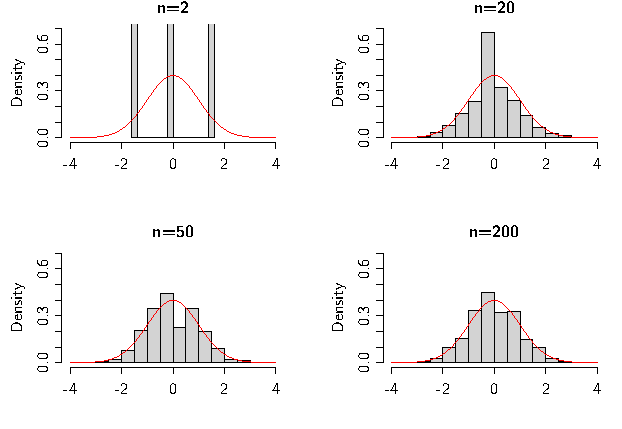
\includegraphics{Resources/Plots/ZGWS-1} 

}

\caption[Zentraler Grenzwertsatz]{Zentraler Grenzwertsatz}\label{fig:ZGWS}
\end{figure}
\normalsize
\end{frame}

\begin{frame}{Überblick}
\protect\hypertarget{uxfcberblick-16}{}
\begin{itemize}
\tightlist
\item
  Wiederholung asymptotischer Theorie
\item
  \textbf{Konsistenz des KQ Schätzers}
\item
  Asymptotische Normalität des KQ Schätzers
\end{itemize}
\end{frame}

\begin{frame}{Konsistenz}
\protect\hypertarget{konsistenz}{}
\begin{itemize}
\tightlist
\item
  Wie gesagt: Betrachten das \alert{lineare Projektionsmodell} \[
  \boxed{\ Y=X^\prime\vbeta+e,\qquad \E[Xe]=\vzero.\ }
  \]
\end{itemize}

\thmn[Hansen (2022, Theorem 7.1)]\label{thm:KQ cons} Im linearen
Projektionsmodell gilt unter den Annahmen \ref{ass:1} und \ref{ass:iid},
dass \[
  \boxed{\ \widehat{\vbeta}\overset{\Pr}{\longrightarrow}\vbeta,\ }
\] d.h.~\(\widehat{\vbeta}\) ist \hil{konsistent} für \(\vbeta\).
\endthmn

\begin{itemize}
\tightlist
\item
  Theorem \ref{thm:KQ cons} besagt: \(\widehat{\vbeta}\) wird \(\vbeta\)
  immer ähnlicher, wenn \(n\to\infty\).
\end{itemize}
\end{frame}

\begin{frame}{Beweis}
\protect\hypertarget{beweis-2}{}
\begin{block}{Beweis von Theorem \ref{thm:KQ cons} (1/3)}
Ausgangspunkt ist \eqref{eq:decomp beta hat}, d.h.
\begin{align*}
  \widehat{\vbeta}-\vbeta &= (\mX^\prime\mX)^{-1}\mX^\prime\ve\\
  &= \Big(\frac{1}{n}\sum_{i=1}^{n}X_i X_i^\prime\Big)^{-1} \Big(\frac{1}{n}\sum_{i=1}^{n}X_i e_i\Big).
\end{align*}
Wir wollen ein GGZ für den \alert{ersten Term} anwenden. Es gilt:
\begin{enumerate}
  \item $X_iX_i^\prime$ ist u.i.v.\ wegen Annahme \ref{ass:iid}.
  \item $\E[X_iX_i^\prime]<\infty$ wegen Annahme \ref{ass:1}.
\end{enumerate}
Wir können also das GGZ (Theorem \ref{thm:GGZ}) anwenden und erhalten
\begin{equation}\label{eq:cons1}
  \frac{1}{n}\sum_{i=1}^{n}X_i X_i^\prime \overset{\Pr}{\longrightarrow} \E[XX^\prime].
\end{equation}
\end{block}
\end{frame}

\begin{frame}{Beweis}
\protect\hypertarget{beweis-3}{}
\begin{block}{Beweis von Theorem \ref{thm:KQ cons} (2/3)}
Ebenso können wir das GGZ (Theorem \ref{thm:GGZ}) auf den \alert{zweiten Term} anwenden:
\begin{equation}\label{eq:cons2}
  \frac{1}{n}\sum_{i=1}^{n}X_i e_i\overset{\Pr}{\longrightarrow}\E[Xe]=\vzero.
\end{equation}
Aus \eqref{eq:cons1}--\eqref{eq:cons2} also wegen \eqref{eq:equiv cj conv}:
\[
  \Big(\frac{1}{n}\sum_{i=1}^{n}X_i X_i^\prime,\ \frac{1}{n}\sum_{i=1}^{n}X_i e_i\Big)\overset{\Pr}{\longrightarrow}\Big(\E[XX^\prime],\ \vzero\Big).
\]
Mit dem CMT 1 folgt dann für $g(\mA,\vb)=\mA^{-1}\vb$:
\[
  \Big(\frac{1}{n}\sum_{i=1}^{n}X_i X_i^\prime\Big)^{-1} \Big(\frac{1}{n}\sum_{i=1}^{n}X_i e_i\Big)\overset{\Pr}{\longrightarrow}\big(\E[XX^\prime]\big)^{-1}\vzero.
\]
Daher also, wie behauptet,
\[
  \widehat{\vbeta}-\vbeta\overset{\Pr}{\longrightarrow}\big(\E[XX^\prime]\big)^{-1}\vzero=\vzero.
\]
\end{block}
\end{frame}

\begin{frame}{Beweis}
\protect\hypertarget{beweis-4}{}
\begin{block}{Beweis von Theorem \ref{thm:KQ cons} (3/3)}
Warum ist $g(\mA,\vb)=\mA^{-1}\vb$ stetig (für die Anwendung von CMT 1)?
\begin{itemize}
  \item $g(\mA,\vb)=\mA^{-1}\vb$ ist stetig in $\mA$ und $\vb$ für alle Werte der Argumente, für die $\mA^{-1}$ existiert.
  \item Wegen Annahme \ref{ass:1} ist $\E[XX^\prime]$ p.d., so dass $(\E[XX^\prime])^{-1}$ existiert. 
  \item Daher ist $g(\mA,\vb)$ stetig in $\mA=\E[XX^\prime]$.
\end{itemize}
\end{block}
\end{frame}

\begin{frame}[fragile,allowframebreaks]{\R Illustration von Konsistenz}
\protect\hypertarget{illustration-von-konsistenz}{}
\xmpl

\begin{itemize}
\tightlist
\item
  Betrachte das Modell \(Y=\beta+e\) mit \(\beta=0\) und
  \(e\sim N(0,1)\).
\item
  Der KQ Schätzer ist dann \(\widehat{\beta}=\overline{Y}_n\).
\end{itemize}

\endxmpl

\footnotesize

\begin{Shaded}
\begin{Highlighting}[]
\NormalTok{Y.bar }\OtherTok{\textless{}{-}} \FunctionTok{matrix}\NormalTok{( }\FunctionTok{rnorm}\NormalTok{(}\DecValTok{4000000}\NormalTok{), }\AttributeTok{nrow=}\DecValTok{20000}\NormalTok{, }\AttributeTok{ncol=}\DecValTok{200}\NormalTok{ )}
\NormalTok{Y.bar }\OtherTok{\textless{}{-}} \FunctionTok{apply}\NormalTok{(Y.bar, }\DecValTok{1}\NormalTok{, }\ControlFlowTok{function}\NormalTok{(x) \{}\FunctionTok{cumsum}\NormalTok{(x)}\SpecialCharTok{/}\DecValTok{1}\SpecialCharTok{:}\FunctionTok{length}\NormalTok{(x)\})}
\NormalTok{x }\OtherTok{\textless{}{-}} \FunctionTok{seq}\NormalTok{(}\SpecialCharTok{{-}}\DecValTok{10}\NormalTok{,}\DecValTok{10}\NormalTok{,}\AttributeTok{by=}\FloatTok{0.02}\NormalTok{)}
\FunctionTok{par}\NormalTok{(}\AttributeTok{mfrow=}\FunctionTok{c}\NormalTok{(}\DecValTok{2}\NormalTok{,}\DecValTok{2}\NormalTok{))}

\CommentTok{\# n=2}
\FunctionTok{hist}\NormalTok{(Y.bar[}\DecValTok{2}\NormalTok{, ],   }\AttributeTok{freq=}\ConstantTok{FALSE}\NormalTok{, }\AttributeTok{main=}\StringTok{"n=2"}\NormalTok{, }\AttributeTok{xlab=}\StringTok{""}\NormalTok{, }\AttributeTok{xlim=}\FunctionTok{c}\NormalTok{(}\SpecialCharTok{{-}}\DecValTok{3}\NormalTok{, }\DecValTok{3}\NormalTok{), }\AttributeTok{ylim=}\FunctionTok{c}\NormalTok{(}\DecValTok{0}\NormalTok{,}\DecValTok{4}\NormalTok{))}
\FunctionTok{abline}\NormalTok{(}\AttributeTok{v=}\DecValTok{0}\NormalTok{, }\AttributeTok{lty=}\StringTok{"dashed"}\NormalTok{)}
\CommentTok{\# n=20}
\FunctionTok{hist}\NormalTok{(Y.bar[}\DecValTok{20}\NormalTok{, ],  }\AttributeTok{freq=}\ConstantTok{FALSE}\NormalTok{, }\AttributeTok{main=}\StringTok{"n=20"}\NormalTok{, }\AttributeTok{xlab=}\StringTok{""}\NormalTok{, }\AttributeTok{xlim=}\FunctionTok{c}\NormalTok{(}\SpecialCharTok{{-}}\DecValTok{3}\NormalTok{, }\DecValTok{3}\NormalTok{), }\AttributeTok{ylim=}\FunctionTok{c}\NormalTok{(}\DecValTok{0}\NormalTok{,}\DecValTok{4}\NormalTok{))}
\FunctionTok{abline}\NormalTok{(}\AttributeTok{v=}\DecValTok{0}\NormalTok{, }\AttributeTok{lty=}\StringTok{"dashed"}\NormalTok{)}
\CommentTok{\# n=50}
\FunctionTok{hist}\NormalTok{(Y.bar[}\DecValTok{50}\NormalTok{, ],  }\AttributeTok{freq=}\ConstantTok{FALSE}\NormalTok{, }\AttributeTok{main=}\StringTok{"n=50"}\NormalTok{, }\AttributeTok{xlab=}\StringTok{""}\NormalTok{, }\AttributeTok{xlim=}\FunctionTok{c}\NormalTok{(}\SpecialCharTok{{-}}\DecValTok{3}\NormalTok{, }\DecValTok{3}\NormalTok{), }\AttributeTok{ylim=}\FunctionTok{c}\NormalTok{(}\DecValTok{0}\NormalTok{,}\DecValTok{4}\NormalTok{))}
\FunctionTok{abline}\NormalTok{(}\AttributeTok{v=}\DecValTok{0}\NormalTok{, }\AttributeTok{lty=}\StringTok{"dashed"}\NormalTok{)}
\CommentTok{\# n=200}
\FunctionTok{hist}\NormalTok{(Y.bar[}\DecValTok{200}\NormalTok{, ], }\AttributeTok{freq=}\ConstantTok{FALSE}\NormalTok{, }\AttributeTok{main=}\StringTok{"n=200"}\NormalTok{, }\AttributeTok{xlab=}\StringTok{""}\NormalTok{, }\AttributeTok{xlim=}\FunctionTok{c}\NormalTok{(}\SpecialCharTok{{-}}\DecValTok{3}\NormalTok{, }\DecValTok{3}\NormalTok{), }\AttributeTok{ylim=}\FunctionTok{c}\NormalTok{(}\DecValTok{0}\NormalTok{,}\DecValTok{4}\NormalTok{))}
\FunctionTok{abline}\NormalTok{(}\AttributeTok{v=}\DecValTok{0}\NormalTok{, }\AttributeTok{lty=}\StringTok{"dashed"}\NormalTok{)}
\end{Highlighting}
\end{Shaded}

\begin{center}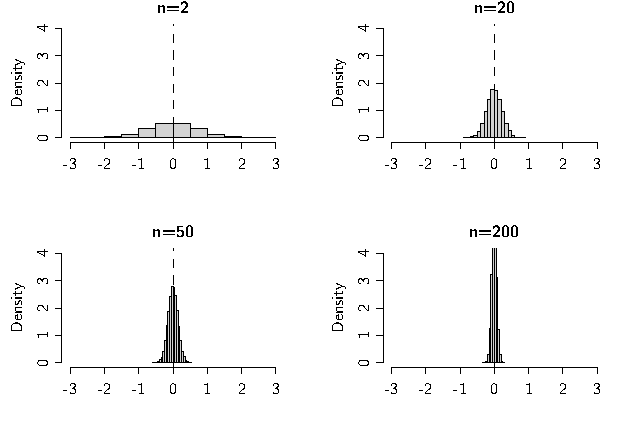
\includegraphics{Resources/Plots/KQ_cons-1} \end{center}
\normalsize
\end{frame}

\begin{frame}[fragile,allowframebreaks]{\R Illustration von
Inkonsistenz}
\protect\hypertarget{illustration-von-inkonsistenz}{}
\framesubtitle{Oder warum Momentenbedingungen wichtig sind}

\xmpl

\begin{itemize}
\tightlist
\item
  Betrachte das Modell \(Y=\beta+e\) mit \(\beta=0\) und
  \(e\sim t_{1.9}\).
\item
  Hier gilt \(\E[Y^2]=\infty\), in Verletzung von Annahme \ref{ass:1}.
\end{itemize}

\endxmpl

\footnotesize

\begin{Shaded}
\begin{Highlighting}[]
\NormalTok{Y.bar }\OtherTok{\textless{}{-}} \FunctionTok{matrix}\NormalTok{( }\FunctionTok{rt}\NormalTok{(}\DecValTok{4000000}\NormalTok{, }\AttributeTok{df=}\FloatTok{1.9}\NormalTok{), }\AttributeTok{nrow=}\DecValTok{20000}\NormalTok{, }\AttributeTok{ncol=}\DecValTok{200}\NormalTok{ )}
\NormalTok{Y.bar }\OtherTok{\textless{}{-}} \FunctionTok{apply}\NormalTok{(Y.bar, }\DecValTok{1}\NormalTok{, }\ControlFlowTok{function}\NormalTok{(x) \{}\FunctionTok{cumsum}\NormalTok{(x)}\SpecialCharTok{/}\DecValTok{1}\SpecialCharTok{:}\FunctionTok{length}\NormalTok{(x)\})}
\NormalTok{x }\OtherTok{\textless{}{-}} \FunctionTok{seq}\NormalTok{(}\SpecialCharTok{{-}}\DecValTok{10}\NormalTok{,}\DecValTok{10}\NormalTok{,}\AttributeTok{by=}\FloatTok{0.02}\NormalTok{)}
\FunctionTok{par}\NormalTok{(}\AttributeTok{mfrow=}\FunctionTok{c}\NormalTok{(}\DecValTok{2}\NormalTok{,}\DecValTok{2}\NormalTok{))}

\CommentTok{\# n=2}
\FunctionTok{hist}\NormalTok{(Y.bar[}\DecValTok{2}\NormalTok{, ],   }\AttributeTok{freq=}\ConstantTok{FALSE}\NormalTok{, }\AttributeTok{main=}\StringTok{"n=2"}\NormalTok{, }\AttributeTok{xlab=}\StringTok{""}\NormalTok{, }\AttributeTok{xlim=}\FunctionTok{c}\NormalTok{(}\SpecialCharTok{{-}}\DecValTok{3}\NormalTok{, }\DecValTok{3}\NormalTok{), }\AttributeTok{ylim=}\FunctionTok{c}\NormalTok{(}\DecValTok{0}\NormalTok{,}\DecValTok{4}\NormalTok{))}
\FunctionTok{abline}\NormalTok{(}\AttributeTok{v=}\DecValTok{0}\NormalTok{, }\AttributeTok{lty=}\StringTok{"dashed"}\NormalTok{)}
\CommentTok{\# n=20}
\FunctionTok{hist}\NormalTok{(Y.bar[}\DecValTok{20}\NormalTok{, ],  }\AttributeTok{freq=}\ConstantTok{FALSE}\NormalTok{, }\AttributeTok{main=}\StringTok{"n=20"}\NormalTok{, }\AttributeTok{xlab=}\StringTok{""}\NormalTok{, }\AttributeTok{xlim=}\FunctionTok{c}\NormalTok{(}\SpecialCharTok{{-}}\DecValTok{3}\NormalTok{, }\DecValTok{3}\NormalTok{), }\AttributeTok{ylim=}\FunctionTok{c}\NormalTok{(}\DecValTok{0}\NormalTok{,}\DecValTok{4}\NormalTok{))}
\FunctionTok{abline}\NormalTok{(}\AttributeTok{v=}\DecValTok{0}\NormalTok{, }\AttributeTok{lty=}\StringTok{"dashed"}\NormalTok{)}
\CommentTok{\# n=50}
\FunctionTok{hist}\NormalTok{(Y.bar[}\DecValTok{50}\NormalTok{, ],  }\AttributeTok{freq=}\ConstantTok{FALSE}\NormalTok{, }\AttributeTok{main=}\StringTok{"n=50"}\NormalTok{, }\AttributeTok{xlab=}\StringTok{""}\NormalTok{, }\AttributeTok{xlim=}\FunctionTok{c}\NormalTok{(}\SpecialCharTok{{-}}\DecValTok{3}\NormalTok{, }\DecValTok{3}\NormalTok{), }\AttributeTok{ylim=}\FunctionTok{c}\NormalTok{(}\DecValTok{0}\NormalTok{,}\DecValTok{4}\NormalTok{))}
\FunctionTok{abline}\NormalTok{(}\AttributeTok{v=}\DecValTok{0}\NormalTok{, }\AttributeTok{lty=}\StringTok{"dashed"}\NormalTok{)}
\CommentTok{\# n=200}
\FunctionTok{hist}\NormalTok{(Y.bar[}\DecValTok{200}\NormalTok{, ], }\AttributeTok{freq=}\ConstantTok{FALSE}\NormalTok{, }\AttributeTok{main=}\StringTok{"n=200"}\NormalTok{, }\AttributeTok{xlab=}\StringTok{""}\NormalTok{, }\AttributeTok{xlim=}\FunctionTok{c}\NormalTok{(}\SpecialCharTok{{-}}\DecValTok{3}\NormalTok{, }\DecValTok{3}\NormalTok{), }\AttributeTok{ylim=}\FunctionTok{c}\NormalTok{(}\DecValTok{0}\NormalTok{,}\DecValTok{4}\NormalTok{))}
\FunctionTok{abline}\NormalTok{(}\AttributeTok{v=}\DecValTok{0}\NormalTok{, }\AttributeTok{lty=}\StringTok{"dashed"}\NormalTok{)}
\end{Highlighting}
\end{Shaded}

\begin{center}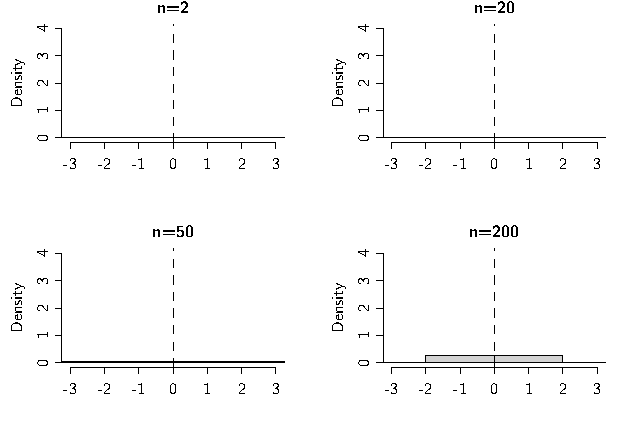
\includegraphics{Resources/Plots/KQ_incons-1} \end{center}
\normalsize
\end{frame}

\begin{frame}{Überblick}
\protect\hypertarget{uxfcberblick-17}{}
\begin{itemize}
\tightlist
\item
  Wiederholung asymptotischer Theorie
\item
  Konsistenz des KQ Schätzers
\item
  \textbf{Asymptotische Normalität des KQ Schätzers}
\end{itemize}
\end{frame}

\begin{frame}{Asymptotische Normalität}
\protect\hypertarget{asymptotische-normalituxe4t}{}
\begin{itemize}
\tightlist
\item
  Konsistenz zeigt
  \(\widehat{\vbeta}-\vbeta\overset{\Pr}{\longrightarrow}\vzero\),
  d.h.~mit \eqref{eq:pr impl d} \[
  \widehat{\vbeta}-\vbeta\overset{d}{\longrightarrow}\vzero.
  \]
\item
  Zum (bspw.) Hypothesentesten reicht das noch nicht aus, weist aber den
  Weg.
\item
  Wir müssen \(\widehat{\vbeta}-\vbeta\) \alert{"aufskalieren"}, um eine
  \alert{nicht-degenerierte Verteilung} zu bekommen.
\item
  Der \alert{"richtige" Faktor} zum Aufskalieren wird (wie im ZGWS)
  \(\sqrt{n}\) sein.
\item
  Um Resultate für \(\sqrt{n}(\widehat{\vbeta}-\vbeta)\) herleiten zu
  können, müssen wir Annahme \ref{ass:1} nachschärfen:\medskip
\end{itemize}

\ass\label{ass:1 ex}

\begin{enumerate}
  \item $\E[Y^4]<\infty$,
  \item $\E[X_i^4]<\infty$ für alle $i$,
  \item $\mQ_{XX^\prime}=\E[XX^\prime]$ ist p.d.
\end{enumerate}
\endass
\end{frame}

\begin{frame}{Asymptotische Normalität}
\protect\hypertarget{asymptotische-normalituxe4t-1}{}
\begin{itemize}
\tightlist
\item
  \alert{Warum} Annahme \ref{ass:1 ex}?
\item
  \alert{Weil} so die Matrix \begin{equation}\label{eq:Omega}
  \mOmega=\Var(Xe)=\E\big[(Xe)(Xe)^\prime\big]=\E[XX^\prime e^2]
  \end{equation} endlich ist: \begin{align}
  \Vert\mOmega\Vert &\leq \E\Vert XX^\prime e^2\Vert\notag\\
    & \leq \E\big[\Vert X\Vert \cdot \Vert X^\prime\Vert e^2\big]\notag\\
    & = \E\big[\Vert X\Vert^2   e^2\big]\label{eq:fin var}\\
    &\leq \Big(\E\Vert X\Vert^4\Big)^{1/2}  \Big(\E[ e^4]\Big)^{1/2}<\infty.\notag
  \end{align}
\item
  Hier haben wir

  \begin{itemize}
  \tightlist
  \item
    im \alert{zweiten Schritt} benutzt, dass die euklidische Norm
    \hil{submultiplikativ} ist,
    d.h.~\(\Vert \mA\mB\Vert\leq \Vert \mA\Vert\cdot\Vert \mB\Vert\),
    und
  \item
    im \alert{vierten Schritt} die \hil{Cauchy--Schwarz Ungleichung}
    \(\E|XY|\leq \sqrt{\E|X|^2 \E|Y|^2}\).
  \end{itemize}
\end{itemize}
\end{frame}

\begin{frame}{Asymptotische Normalität}
\protect\hypertarget{asymptotische-normalituxe4t-2}{}
\thmn[Asymptotische Normalität von $\widehat{\vbeta}$]\label{thm:KQ AN}
Im linearen Projektionsmodell gilt unter den Annahmen \ref{ass:iid} und
\ref{ass:1 ex}, dass \[
  \boxed{\ \sqrt{n}\big(\widehat{\vbeta}-\vbeta\big)\overset{d}{\longrightarrow}N(\vzero, \mV_{\vbeta}),\ }
\] wobei
\(\mV_{\vbeta}=\mQ^{-1}_{XX^\prime}\mOmega\mQ^{-1}_{XX^\prime}\) die
\hil{asymptotische Varianz} von \(\widehat{\vbeta}\) ist. \endthmn

\begin{itemize}
\tightlist
\item
  \alert{Wahnsinn:} Egal welche Verteilung die Regressoren, Regressanden
  oder Fehler haben, der KQ Schätzer ist immer asymptotisch
  normalverteilt!!!
\item
  Aus offensichtlichen Gründen sagen wir, dass \(\mV_{\vbeta}\)
  \hil{Sandwich Form} hat:

  \begin{itemize}
  \tightlist
  \item
    \(\mOmega\) ist das \hil{Meat} und
  \item
    \(\mQ^{-1}_{XX^\prime}\) ist das \hil{Bread}.
  \end{itemize}
\end{itemize}
\end{frame}

\begin{frame}{Beweis}
\protect\hypertarget{beweis-5}{}
\begin{block}{Beweis von Theorem \ref{thm:KQ AN} (1/3)}
Ausgangspunkt ist wieder \eqref{eq:decomp beta hat}, d.h.
\begin{equation*}
  \sqrt{n}\big(\widehat{\vbeta}-\vbeta\big) = \Big(\frac{1}{n}\sum_{i=1}^{n}X_i X_i^\prime\Big)^{-1} \Big(\frac{1}{\sqrt{n}}\sum_{i=1}^{n}X_i e_i\Big).
\end{equation*}
Haben bereits im Beweis von Theorem \ref{thm:KQ cons} gesehen:
\begin{equation}\label{eq:convXX}
  \Big(\frac{1}{n}\sum_{i=1}^{n}X_i X_i^\prime\Big)^{-1}\overset{\Pr}{\longrightarrow}\mQ_{XX^\prime}^{-1}.
\end{equation}
Also müssen wir uns nur noch um den \alert{zweiten Term} kümmern...

\end{block}
\end{frame}

\begin{frame}{Beweis}
\protect\hypertarget{beweis-6}{}
\begin{block}{Beweis von Theorem \ref{thm:KQ AN} (2/3)}
Für $\frac{1}{\sqrt{n}}\sum_{i=1}^{n}X_i e_i$ können wir den ZGWS (Theorem \ref{thm:ZGWS}) anwenden, denn:
\begin{enumerate}
  \item $X_i e_i=X_i(Y_i-X_i^\prime\vbeta)$ ist u.i.v.\ als Funktion von u.i.v.\ Variablen (Annahme \ref{ass:iid}).
  \item $\E\big[\Vert X e\Vert^2\big]=\E\big[\Vert X\Vert^2 e^2\big]<\infty$, wie unter \eqref{eq:fin var}.\medskip
\end{enumerate}

Theorem \ref{thm:ZGWS} impliziert daher:
\begin{equation}\label{eq:error CLT}
  \frac{1}{\sqrt{n}}\sum_{i=1}^{n}X_i e_i\overset{d}{\longrightarrow}N(\vzero,\mOmega).
\end{equation}

(Erinnern Sie sich, dass im linearen Projektionsmodell $\vmu=\E[X_ie_i]=\vzero$ gilt.)
\end{block}
\end{frame}

\begin{frame}{Beweis}
\protect\hypertarget{beweis-7}{}
\begin{block}{Beweis von Theorem \ref{thm:KQ AN} (3/3)}
Kombiniere \eqref{eq:convXX} und \eqref{eq:error CLT} mit dem Satz von Slutzky:
\begin{align*}
  \sqrt{n}\big(\widehat{\vbeta}-\vbeta\big) &= \Big(\frac{1}{n}\sum_{i=1}^{n}X_i X_i^\prime\Big)^{-1} \Big(\frac{1}{\sqrt{n}}\sum_{i=1}^{n}X_i e_i\Big)\\
  &\overset{d}{\longrightarrow} \mQ^{-1}_{XX^\prime}N(\vzero,\mOmega).
\end{align*}

Da Linearkombinationen normalverteilter Zufallsvektoren wieder normalverteilt sind, gilt
\begin{align*}
  \mQ^{-1}_{XX^\prime}N(\vzero,\mOmega)&\overset{d}{=}N\big(\vzero,\mQ^{-1}_{XX^\prime}\mOmega(\mQ^{-1}_{XX^\prime})^\prime\big)\\
  &=N\big(\vzero,\mQ^{-1}_{XX^\prime}\mOmega(\mQ^{\prime}_{XX^\prime})^{-1}\big)\\
  &=N(\vzero,\mQ^{-1}_{XX^\prime}\mOmega\mQ^{-1}_{XX^\prime}),
\end{align*}
wobei der vorletzte Schritt aus Proposition\ \zref{S-rules3}.\zref{S-it:21.3} und der letzte aus Symmetrie von $\mQ_{XX^\prime}$ folgt (d.h. $\mQ_{XX^\prime}^\prime=\mQ_{XX^\prime}$).
\end{block}
\end{frame}

\begin{frame}{\R Illustration}
\protect\hypertarget{illustration}{}
\xmpl

\begin{itemize}
\tightlist
\item
  Betrachte das Modell \(Y=\beta+e\) für \[
  e=\frac{u^r-\E[u^r]}{\Big(\E[u^{2r}] - \big(\E[u^r]\big)^2\Big)^{1/2}},\qquad u\sim N(0,1).
  \]

  \begin{itemize}
  \tightlist
  \item
    Insbesondere gilt \(e\sim(0,1)\), d.h.~\(\E[e]=0\) und
    \(\Var(e)=1\).
  \end{itemize}
\item
  Wir zeigen die \alert{Verteilung} von
  \(\sqrt{n}(\widehat{\beta}-\beta)\) für \(n=100\) und verschiedene
  Werte von \(r=1,4,6\) und \(8\).
\item
  \alert{Lektion:} Die Normalverteilungsapproximation ist nicht immer
  akkurat in endlichen Stichproben!
\end{itemize}

\endxmpl
\end{frame}

\begin{frame}[fragile]{\R Illustration}
\protect\hypertarget{illustration-1}{}
\footnotesize

\begin{Shaded}
\begin{Highlighting}[]
\NormalTok{r }\OtherTok{\textless{}{-}} \DecValTok{100000}
\NormalTok{n }\OtherTok{\textless{}{-}} \DecValTok{100}
\NormalTok{k\_vec }\OtherTok{\textless{}{-}} \FunctionTok{c}\NormalTok{(}\DecValTok{8}\NormalTok{,}\DecValTok{6}\NormalTok{,}\DecValTok{4}\NormalTok{)}
\NormalTok{x }\OtherTok{\textless{}{-}} \FunctionTok{seq}\NormalTok{(}\SpecialCharTok{{-}}\FloatTok{2.5}\NormalTok{,}\FloatTok{2.5}\NormalTok{,.}\DecValTok{01}\NormalTok{)}
\NormalTok{xn }\OtherTok{\textless{}{-}} \FunctionTok{length}\NormalTok{(x)}

\NormalTok{f }\OtherTok{\textless{}{-}} \FunctionTok{matrix}\NormalTok{(}\DecValTok{0}\NormalTok{,xn,}\DecValTok{5}\NormalTok{)}
\ControlFlowTok{for}\NormalTok{ (i }\ControlFlowTok{in} \DecValTok{1}\SpecialCharTok{:}\DecValTok{3}\NormalTok{)\{}
\NormalTok{  k }\OtherTok{\textless{}{-}}\NormalTok{ k\_vec[i]}
\NormalTok{  m1 }\OtherTok{\textless{}{-}} \FunctionTok{prod}\NormalTok{(}\FunctionTok{seq}\NormalTok{(}\AttributeTok{from=}\DecValTok{1}\NormalTok{,}\AttributeTok{by=}\DecValTok{2}\NormalTok{,}\AttributeTok{length.out=}\NormalTok{k}\SpecialCharTok{/}\DecValTok{2}\NormalTok{))}
\NormalTok{  m2 }\OtherTok{\textless{}{-}} \FunctionTok{prod}\NormalTok{(}\FunctionTok{seq}\NormalTok{(}\AttributeTok{from=}\DecValTok{1}\NormalTok{,}\AttributeTok{by=}\DecValTok{2}\NormalTok{,}\AttributeTok{length.out=}\NormalTok{k))}
\NormalTok{  y }\OtherTok{\textless{}{-}}  \FunctionTok{matrix}\NormalTok{(}\FunctionTok{rnorm}\NormalTok{(n}\SpecialCharTok{*}\NormalTok{r),n,r)}\SpecialCharTok{\^{}}\NormalTok{k}
\NormalTok{  y1 }\OtherTok{\textless{}{-}}\NormalTok{ (y}\SpecialCharTok{{-}}\NormalTok{m1)}\SpecialCharTok{/}\FunctionTok{sqrt}\NormalTok{(m2}\SpecialCharTok{{-}}\NormalTok{m1}\SpecialCharTok{\^{}}\DecValTok{2}\NormalTok{)}
\NormalTok{  beta }\OtherTok{\textless{}{-}} \FunctionTok{colMeans}\NormalTok{(y1)}\SpecialCharTok{*}\FunctionTok{sqrt}\NormalTok{(n)}
\NormalTok{  bd }\OtherTok{\textless{}{-}}\NormalTok{ .}\DecValTok{7}\SpecialCharTok{*}\FunctionTok{sd}\NormalTok{(beta)}\SpecialCharTok{/}\NormalTok{(r}\SpecialCharTok{\^{}}\NormalTok{(.}\DecValTok{2}\NormalTok{))}
  \ControlFlowTok{for}\NormalTok{ (j }\ControlFlowTok{in} \DecValTok{1}\SpecialCharTok{:}\NormalTok{xn)\{}
\NormalTok{    xj }\OtherTok{\textless{}{-}}\NormalTok{ x[j]}
\NormalTok{    f[j,i] }\OtherTok{\textless{}{-}} \FunctionTok{mean}\NormalTok{(}\FunctionTok{dnorm}\NormalTok{((beta}\SpecialCharTok{{-}}\NormalTok{xj)}\SpecialCharTok{/}\NormalTok{bd))}\SpecialCharTok{/}\NormalTok{bd}
\NormalTok{  \}}
\NormalTok{\}}
\NormalTok{f[,}\DecValTok{4}\NormalTok{] }\OtherTok{\textless{}{-}} \FunctionTok{dnorm}\NormalTok{(x)}

\NormalTok{wd }\OtherTok{=} \FloatTok{1.4}
\end{Highlighting}
\end{Shaded}

\normalsize
\end{frame}

\begin{frame}[fragile,allowframebreaks]{\R Illustration}
\protect\hypertarget{illustration-2}{}
\footnotesize

\begin{Shaded}
\begin{Highlighting}[]
\NormalTok{leg1 }\OtherTok{\textless{}{-}} \FunctionTok{expression}\NormalTok{(}\StringTok{\textquotesingle{}N(0,1)\textquotesingle{}}\SpecialCharTok{\^{}}\DecValTok{8}\NormalTok{)}
\NormalTok{leg2 }\OtherTok{\textless{}{-}} \FunctionTok{expression}\NormalTok{(}\StringTok{\textquotesingle{}N(0,1)\textquotesingle{}}\SpecialCharTok{\^{}}\DecValTok{6}\NormalTok{)}
\NormalTok{leg3 }\OtherTok{\textless{}{-}} \FunctionTok{expression}\NormalTok{(}\StringTok{\textquotesingle{}N(0,1)\textquotesingle{}}\SpecialCharTok{\^{}}\DecValTok{4}\NormalTok{)}
\NormalTok{leg4 }\OtherTok{\textless{}{-}} \FunctionTok{expression}\NormalTok{(}\StringTok{\textquotesingle{}N(0,1)\textquotesingle{}}\NormalTok{)}
\NormalTok{leg }\OtherTok{\textless{}{-}} \FunctionTok{c}\NormalTok{(leg1,leg2,leg3,leg4)}


\FunctionTok{plot}\NormalTok{(x,f[,}\DecValTok{1}\NormalTok{], }\AttributeTok{type=}\StringTok{"l"}\NormalTok{,}\AttributeTok{lty=}\DecValTok{5}\NormalTok{,}\AttributeTok{xlab=}\StringTok{""}\NormalTok{,}\AttributeTok{ylab=}\StringTok{""}\NormalTok{,}\AttributeTok{ylim=}\FunctionTok{c}\NormalTok{(}\DecValTok{0}\NormalTok{,}\FloatTok{1.4}\NormalTok{),}\AttributeTok{xaxs=}\StringTok{"i"}\NormalTok{,}\AttributeTok{yaxs=}\StringTok{"i"}\NormalTok{,}\AttributeTok{bty=}\StringTok{"n"}\NormalTok{,}\AttributeTok{xaxt=}\StringTok{"n"}\NormalTok{,}\AttributeTok{yaxt=}\StringTok{"n"}\NormalTok{,}\AttributeTok{lwd=}\NormalTok{wd)}
\FunctionTok{lines}\NormalTok{(x,f[,}\DecValTok{2}\NormalTok{],}\AttributeTok{lty=}\DecValTok{6}\NormalTok{,}\AttributeTok{lwd=}\NormalTok{wd)}
\FunctionTok{lines}\NormalTok{(x,f[,}\DecValTok{3}\NormalTok{],}\AttributeTok{lty=}\DecValTok{2}\NormalTok{,}\AttributeTok{lwd=}\NormalTok{wd)}
\FunctionTok{lines}\NormalTok{(x,f[,}\DecValTok{4}\NormalTok{],}\AttributeTok{lty=}\DecValTok{1}\NormalTok{,}\AttributeTok{lwd=}\NormalTok{wd)}
\FunctionTok{axis}\NormalTok{(}\DecValTok{1}\NormalTok{,}\FunctionTok{seq}\NormalTok{(}\SpecialCharTok{{-}}\DecValTok{3}\NormalTok{,}\DecValTok{3}\NormalTok{,}\DecValTok{1}\NormalTok{),}\AttributeTok{lwd=}\NormalTok{wd)}
\FunctionTok{legend}\NormalTok{(}\StringTok{"topright"}\NormalTok{,}\AttributeTok{legend=}\NormalTok{leg,}\AttributeTok{lty=}\FunctionTok{c}\NormalTok{(}\DecValTok{5}\NormalTok{,}\DecValTok{6}\NormalTok{,}\DecValTok{2}\NormalTok{,}\DecValTok{1}\NormalTok{),}\AttributeTok{lwd=}\NormalTok{wd,}\AttributeTok{bty=}\StringTok{"n"}\NormalTok{)}
\end{Highlighting}
\end{Shaded}

\begin{center}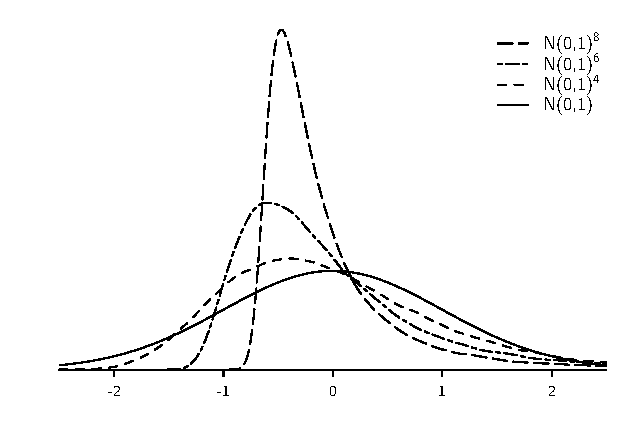
\includegraphics{Resources/Plots/InNor2-1} \end{center}
\normalsize
\end{frame}

\begin{frame}{Diskussion von Theorem \ref{thm:KQ AN}}
\protect\hypertarget{diskussion-von-theorem}{}
\begin{itemize}
\tightlist
\item
  Es ist interessant, die asymptotische Varianz \(\mV_{\vbeta}\) der
  Verteilung von \(\sqrt{n}(\widehat{\vbeta}-\vbeta)\) mit der Varianz
  des KQ Schätzers im linearen bedingten Erwartungswertmodell zu
  \alert{vergleichen} (siehe Theorem \ref{thm:Var KQ}): \[
  \mV_{\widehat{\vbeta}} := \Var(\widehat{\vbeta}\mid \mX) = (\mX^\prime\mX)^{-1}(\mX^\prime\mD\mX) (\mX^\prime\mX)^{-1}. 
  \]
\item
  Also: \[
  \mV_{\vbeta}\approx\Var\big(\sqrt{n}(\widehat{\vbeta}-\vbeta)\big)=n\Var(\widehat{\vbeta})\approx n\Var(\widehat{\vbeta}\mid\mX)=n\mV_{\widehat{\vbeta}}.
  \]
\item
  Das motiviert als Schätzer von \(\mV_{\vbeta}\): \[
  n\mV_{\widehat{\vbeta}}=\Big(\frac{1}{n}\mX^\prime\mX\Big)^{-1}\Big(\frac{1}{n}\mX^\prime\mD\mX\Big) \Big(\frac{1}{n}\mX^\prime\mX\Big)^{-1}
  \]
\item
  Dieser wird im folgenden Kapitel zur Inferenz wichtig, da \alert{nur}
  zu wissen, dass \(\sqrt{n}(\widehat{\vbeta}-\vbeta)\) asymptotisch
  normal ist, uns nicht weiter hilft, wenn wir nicht auch die
  \alert{Varianz} kennen (oder zumindest schätzen können)\ldots{}
\end{itemize}
\end{frame}

\hypertarget{inferenz}{%
\section{Inferenz}\label{inferenz}}

\begin{frame}{}
\protect\hypertarget{section-5}{}
\centerline{\textbf{Inferenz}}
\centerline{(Hansen, 2022, Kapitel 7 \& 9)}
\end{frame}

\begin{frame}{Ausblick}
\protect\hypertarget{ausblick-1}{}
\begin{itemize}
\tightlist
\item
  \alert{Im vorherigen Kapitel:} Haben etwas über die Verteilung von
  \(\widehat{\vbeta}\) in großen Stichproben gelernt.
\item
  \alert{Jetzt:} Wollen das anwenden, um
  \alert{Hypothesentests, Konfidenzintervalle, etc.} zu konstruieren.
\item
  Alles funktioniert wieder für das (allgemeinste)
  \alert{lineare Projektionsmodell}.
\end{itemize}
\end{frame}

\begin{frame}{Überblick}
\protect\hypertarget{uxfcberblick-18}{}
\begin{itemize}
\tightlist
\item
  \textbf{Wiederholung Testtheorie}
\item
  Bedingte Homoskedastie
\item
  Bedingte Heteroskedastie
\item
  Hypothesentests
\item
  Konfidenzintervalle
\end{itemize}
\end{frame}

\begin{frame}{Motivation}
\protect\hypertarget{motivation-1}{}
\begin{itemize}
\tightlist
\item
  \alert{Warum} brauchen wir Testtheorie?
\item
  \alert{Weil} es ein Glückstreffer wäre, wenn \(\widehat{\vbeta}\) dem
  wahren Wert \(\vbeta\) in einer endlichen Stichprobe entspräche.
\item
  Daher müssen wir die \alert{Zufälligkeit} von \(\widehat{\vbeta}\) mit
  einbeziehen, wenn wir Schlussfolgerungen über \(\vbeta\) ziehen
  wollen.
\item
  \alert{Großartig:} Testtheorie erlaubt uns, Schlüsse aus Daten zu
  ziehen, die die Zufälligkeit der Stichprobe berücksichtigen.
\item
  Wir präsentieren Testtheorie hier für den Parameter von Interesse \[
  \vtheta=\vr(\vbeta),\qquad \vr:\mathbb{R}^{k}\mapsto\mathbb{R}^{p}.
  \]

  \begin{itemize}
  \tightlist
  \item
    \alert{Beispiele:} \(\vtheta=\beta_j\),
    \(\vtheta=\beta_j-\beta_{\ell}\), \(\vtheta=\beta_j/\beta_{\ell}\).
  \end{itemize}
\end{itemize}
\end{frame}

\begin{frame}{Hypothesen}
\protect\hypertarget{hypothesen}{}
\defn[Hypothesen]Die \hil{Nullhypothese} (kurz: \hil{Null})
\(\mathbb{H}_0\) ist die Restriktion \(\vtheta=\vtheta_0\).\bigskip

Die \hil{Alternativhypothese} (kurz: \hil{Alternative}) \(\mathbb{H}_1\)
kann entweder zweiseitig sein (\(\vtheta\neq\vtheta_0\)) oder einseitig
(\(\vtheta>\vtheta_0\) oder \(\vtheta<\vtheta_0\) komponentenweise).
\enddefn

\begin{itemize}
\tightlist
\item
  Die Null ist meist (wie hier) eine \hil{einfache} Hypothese, während
  die Alternative \hil{zusammengesetzt} ist.
\item
  \alert{Ziel} von Hypothesentests: Sind die beobachteten Daten
  konsistent mit \(\mathbb{H}_0\)? Ja (``akzeptiere \(\mathbb{H}_0\)'')
  oder Nein (``verwirf \(\mathbb{H}_0\)'').
\item
  Um das zu entscheiden, teilen wir den Raum aller möglichen Stichproben
  in eine \hil{Annahmeregion} \(S_0\) und eine \hil{Ablehnregion}
  \(S_1\).
\end{itemize}
\end{frame}

\begin{frame}{Teststatistik und kritische Werte}
\protect\hypertarget{teststatistik-und-kritische-werte}{}
\begin{itemize}
\tightlist
\item
  Die Teilung des Stichprobenraums erfolgt via einer reellwertigen
  \hil{Teststatistik} \[
  T=T\big((Y_1,X_1),\ldots,(Y_n, X_n)\big)
  \] und einem \hil{kritischen Wert} \(c\).
\item
  Ideal: \alert{Kleine} Werte von \(T\) sind wahrscheinlich unter
  \(\mathbb{H}_0\) und \alert{große} Werte von \(T\) sind wahrscheinlich
  unter \(\mathbb{H}_1\).
\end{itemize}

\footnotesize
\begin{center}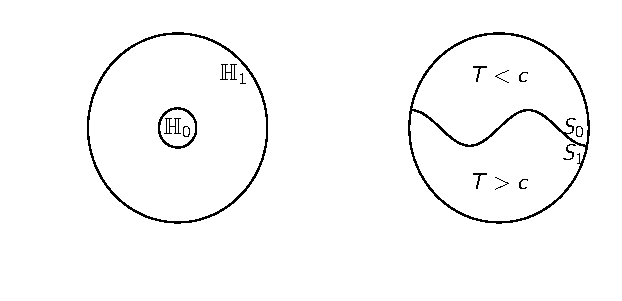
\includegraphics{Resources/Plots/Illu_test-1} \end{center}
\normalsize
\end{frame}

\begin{frame}{Teststatistik und kritische Werte}
\protect\hypertarget{teststatistik-und-kritische-werte-1}{}
\xmpl

\begin{itemize}
\tightlist
\item
  Im Modell \[
  Y_i=\beta+e_i,\qquad e_i\overset{\text{u.i.v.}}{\sim}N(0,\sigma^2)
  \] gilt \[
  \widehat{\beta}=\overline{Y}_n,\quad\Var(\widehat{\beta})=\sigma^2/n.
  \]
\item
  Eine geeignete Teststatistik (bei bekanntem \(\sigma\)) für die Null
  \(\mathbb{H}_0\colon \beta=\beta_0\) ist der Absolutwert der
  \hil{$t$-Statistik} \[
  T=T(Y_1,\ldots,Y_n)=|t(Y_1,\ldots,Y_n)|=\frac{\big|\overline{Y}_n-\beta_0\big|}{\sigma/\sqrt{n}}.
  \]
\item
  Die Wahl eines (geeigneten, s.u.) kritischen Werts \(c\) teilt dann
  den Stichprobenraum in Annahmeregion \(S_0\) und Ablehnregion \(S_1\).
\end{itemize}

\endxmpl
\end{frame}

\begin{frame}{Fehler 1.~Art}
\protect\hypertarget{fehler-1.-art}{}
\defn[\hil{Fehler 1.\ Art}]Die Null fälschlicherweise abzulehnen
(\(\mathbb{H}_0\) abzulehnen, obwohl \(\mathbb{H}_0\) wahr) ist ein
\hil{Fehler 1.\ Art}.\medskip

Die Wahrscheinlichkeit eines Fehlers 1.~Art nennen wir das
\hil{Signifikanzniveau} des Tests: \[
  \Pr\big\{\text{Verwirf}\ \mathbb{H}_0 \mid \mathbb{H}_0\ \text{ist wahr}\big\}=\Pr\big\{T>c\mid \mathbb{H}_0\ \text{ist wahr}\big\}.
\] Das \hil{asymptotische Signifikanzniveau} eines Tests ist \[
  \lim_{n\to\infty}\Pr\big\{T>c\mid \mathbb{H}_0\ \text{ist wahr}\big\}.
\] \enddefn

\begin{itemize}
\tightlist
\item
  Im Folgenden am \alert{häufigsten:} Kontrolle des
  \alert{asymptotischen Signifikanzniveaus}, weil wir unter
  \(\mathbb{H}_0\) nur haben \[
  T\overset{d}{\longrightarrow} \xi,\qquad n\to\infty.
  \]
\item
  Die Verteilung \(G(u)=\Pr\{\xi\leq u\}\) nennen wir die
  \hil{asymptotische Nullverteilung}
\end{itemize}
\end{frame}

\begin{frame}{Fehler 2.~Art}
\protect\hypertarget{fehler-2.-art}{}
\begin{itemize}
\tightlist
\item
  Nur das Niveau einzuhalten ist \alert{keine Kunst}.

  \begin{itemize}
  \tightlist
  \item
    Generiere eine rechteckverteilte ``Teststatistik''
    \(T \sim U[0,1]\).
  \item
    Ein Test, der \emph{immer} ablehnt wenn \(T>1-\alpha\), ist per
    Konstruktion ein Test z.N.~\(\alpha\) für \alert{jedes Testproblem},
    \ldots{}
  \item
    \ldots{} aber wir können nichts aus ihm lernen.
  \end{itemize}
\item
  Ein guter Test braucht \alert{Macht:}\medskip
\end{itemize}

\defn[Fehler 2.\ Art]Die Null fälschlicherweise zu akzeptieren
(\(\mathbb{H}_0\) annehmen, obwohl \(\mathbb{H}_1\) wahr) ist ein
\hil{Fehler 2.\ Art}.\medskip

Die Wahrscheinlichkeit \(H_0\) abzulehnen, wenn \(H_1\) wahr ist, heißt
\hil{Macht}: \[
  \Pr\big\{\text{Verwirf}\ \mathbb{H}_0\mid \mathbb{H}_1\ \text{ist wahr}\big\}.
\] \enddefn

\begin{itemize}
\tightlist
\item
  Dominanter Ansatz in Statistik: Will Test mit hoher Macht, der
  \alert{vorspezifiziertes} Signifikanzniveau einhält.
\end{itemize}
\end{frame}

\begin{frame}{Fehler 1.~und 2.~Art}
\protect\hypertarget{fehler-1.-und-2.-art}{}
\begin{itemize}
\tightlist
\item
  Es gibt \alert{zwei} Zustände der Wirklichkeit (\(\mathbb{H}_0\) oder
  \(\mathbb{H}_1\)) und \alert{zwei} Entscheidungen (akzeptiere
  \(\mathbb{H}_0\) oder verwirf \(\mathbb{H}_0\)).
\item
  Insgesamt können also \alert{4 Dinge} eintreten:
\end{itemize}

\begin{center}
\begin{tabular}{|l|c|c|}\hline
\diaghead{\theadfont Diag ColumnmnHead}%
{Entscheidung}{Wirklichkeit}&
\thead{$\mathbb{H}_0$ wahr}&\thead{$\mathbb{H}_0$ falsch}\\
\hline
Akzeptiere $\mathbb{H}_0$ & korrekt     & Fehler 2.\ Art \\
\hline
Verwirf $\mathbb{H}_0$      & Fehler 1.\ Art    & korrekt \\
\hline
\end{tabular}
\end{center}
\end{frame}

\begin{frame}{Fehler 1.~und 2.~Art}
\protect\hypertarget{fehler-1.-und-2.-art-1}{}
\xmpl[Fortsetzung]\label{ex:Error types}

\begin{itemize}
\tightlist
\item
  Da die \(t\)-Statistik standardnormalverteilt ist, gilt für die
  Teststatistik \begin{equation}\label{eq:t ex distr}
   T\sim|N(0,1)|.
  \end{equation}
\item
  Wählen wir also \(c=c_{\alpha}=\Phi^{-1}(1-\alpha/2)\), dann gilt für
  das \alert{Signifikanzniveau} \begin{align*}
  \Pr\big\{\text{Verwirf}\ \mathbb{H}_0 \mid \mathbb{H}_0\ \text{ist wahr}\big\} &= \Pr\big\{T>c\mid \mathbb{H}_0\ \text{ist wahr}\big\}\\
  &= \Pr\big\{|N(0,1)|>c_{\alpha}\big\}\\
  &= \Phi(-c_{\alpha}) + \big[1-\Phi(c_{\alpha})\big]\\
  &= \alpha/2 + \big[1-(1-\alpha/2)\big]\\
  &=\alpha.
  \end{align*}
\item
  Die \alert{Macht} eines Tests ist i.A.~schwierig zu berechnen -- man
  hofft meist, dass sie groß ist.
\end{itemize}

\endxmpl
\end{frame}

\begin{frame}{\(p\)-Wert}
\protect\hypertarget{p-wert}{}
\begin{itemize}
\tightlist
\item
  Ein Test der Null kennt nur die \alert{beiden} Ergebnisse ``Akzeptiere
  \(\mathbb{H}_0\)'' und ``Verwirf \(\mathbb{H}_0\)''.
\item
  Das ist \alert{keine gute Zusammenfassung der Evidenz} für oder gegen
  die Null!

  \begin{itemize}
  \tightlist
  \item
    Beispiel \ref{ex:Error types}: \(T=500\) liefert größere Evidenz
    gegen \(\mathbb{H}_0\colon\beta=\beta_0\) als \(T=2.1\).
  \end{itemize}
\item
  Eine bessere Zusammenfassung liefert der \(p\)-Wert:\medskip
\end{itemize}

\defn[$p$-Wert]Der \hil{(asymptotische) $p$-Wert} ist die
Zufallsvariable \begin{equation*}
  p = 1-G\big(T\big((Y_1,X_1),\ldots,(Y_n,X_n)\big)\big),
\end{equation*} wobei \(G(\cdot)\) die asymptotische Nullverteilung der
Teststatistik ist. \enddefn

\begin{itemize}
\tightlist
\item
  Der \(p\)-Wert ist eine \alert{äquivalente Teststatistik}, weil unter
  \(\mathbb{H}_0\) (prüfen Sie es nach!): \[
  T>c\ \text{mit asympt. Wkt.}\ \alpha\qquad\Longleftrightarrow\qquad p<\alpha\ \text{mit asympt. Wkt.}\ \alpha.
  \]
\end{itemize}
\end{frame}

\begin{frame}{\(p\)-Wert}
\protect\hypertarget{p-wert-1}{}
\[
   \boxed{\ T>c\ \text{mit asympt. Wkt.}\ \alpha\qquad\Longleftrightarrow\qquad p<\alpha\ \text{mit asympt. Wkt.}\ \alpha\ }
\]

\begin{itemize}
\tightlist
\item
  Wir zeigen hier nur ``\(\Longrightarrow\)''.
\item
  Dann gilt \begin{equation}\label{eq:hyp}
   \Pr\big\{T>c\mid\mathbb{H}_0\ \text{ist wahr}\big\} \underset{(n\to\infty)}{\longrightarrow}\alpha=\Pr\{\xi>c\}=1-G(c).
  \end{equation}
\item
  Also auch \begin{eqnarray*}
   \Pr\big\{p<\alpha\mid\mathbb{H}_0\ \text{ist wahr}\big\}&\overset{\eqref{eq:hyp}}{=}& \Pr\{p<1-G(c)\mid\mathbb{H}_0\ \text{ist wahr}\}\\
   &=& \Pr\big\{1-G(T)<1-G(c)\mid\mathbb{H}_0\ \text{ist wahr}\big\}\\
   &=& \Pr\big\{G(T)>G(c)\mid\mathbb{H}_0\ \text{ist wahr}\big\}\\
   &=& \Pr\big\{T>c\mid\mathbb{H}_0\ \text{ist wahr}\big\}\underset{(n\to\infty)}{\overset{\eqref{eq:hyp}}{\longrightarrow}}\alpha.
  \end{eqnarray*}
\item
  ÜA: Zeigen Sie, dass auch die Rückrichtung (``\(\Longleftarrow\)'')
  gilt.
\end{itemize}
\end{frame}

\begin{frame}{\(p\)-Wert}
\protect\hypertarget{p-wert-2}{}
\begin{itemize}
\tightlist
\item
  Der große Vorteil des \(p\)-Wertes ist seine
  \alert{Normierung:}\medskip
\end{itemize}

\thmn[Hansen (2022, p. 231)]\label{thm:p-Wert} Gelte
\(T\overset{d}{\longrightarrow}\xi\) unter \(\mathbb{H}_0\), wobei die
asymptotische Nullverteilung \(G(\cdot)\) streng monoton steigt und
stetig ist. Dann gilt \[
  p\overset{d}{\longrightarrow} U[0,1].
\] \endthmn

\begin{itemize}
\tightlist
\item
  Wegen dieser Normierung ist die \alert{"Ungewöhnlichkeit" von $p$}
  einfacher zu interpretieren als die ``Ungewöhnlichkeit'' von \(T\).
\item
  Der \(p\)-Wert wird oft auch das \hil{marginale Signifikanzniveau}
  genannt: Der kleinste Wert von \(\alpha\) für den ein Test basierend
  auf \(T\) die Null ablehnt.

  \begin{itemize}
  \tightlist
  \item
    \(p=0.11\) heißt \(T\) lehnt \(\mathbb{H}_0\) zu Niveaus
    \(\alpha>0.11\) ab, \ldots{}
  \item
    \ldots{} aber verwirft nicht für Niveaus \(\alpha<0.11\).
  \end{itemize}
\end{itemize}
\end{frame}

\begin{frame}{\(p\)-Wert}
\protect\hypertarget{p-wert-3}{}
\begin{block}{Beweis von Theorem \ref{thm:p-Wert}}
Das CMT 2 und $T\overset{d}{\longrightarrow}\xi$ implizieren, dass 
\[
  p=1-G(T) \overset{d}{\longrightarrow}1-G(\xi).
\]
Die Verteilung von $1-G(\xi)$ ist die $U[0,1]$-Verteilung, denn
\begin{align*}
  \Pr\{1-G(\xi)\leq u\} &= \Pr\{1-u\leq G(\xi)\}\\
  &= \Pr\{G^{-1}(1-u)\leq \xi \}\\
  &= 1-\Pr\{\xi\leq G^{-1}(1-u)\}\\
  &= 1- G\big(G^{-1}(1-u)\big)\\
  &= 1-(1-u)\\
  &= u.
\end{align*}
Wir haben also gezeigt, dass
\[
  p\overset{d}{\longrightarrow}U[0,1].
\]
\end{block}
\end{frame}

\begin{frame}{\(p\)-Wert}
\protect\hypertarget{p-wert-4}{}
\begin{quote}
\glqq ... surely, God loves the .06 nearly as much as the .05. Can there be any doubt that God views the strength of evidence for or against the null as a fairly continuous function of the magnitude of p?\grqq{} \textup{---Rosnow, R. L., \& Rosenthal, R. (1989). Statistical procedures and the justification of knowledge in psychological science. American Psychologist, 44(10), 1276-1284.}\\[2ex]
\end{quote}

\begin{itemize}
\tightlist
\item
  Ein verwandtes Problem:

  \begin{center}
  
\includegraphics[width=3cm,keepaspectratio=true]{"Resources/p_values.png"}
  \end{center}
\end{itemize}
\end{frame}

\begin{frame}{\(p\)-Wert}
\protect\hypertarget{p-wert-5}{}
\xmpl[Fortsetzung]\label{ex:p val}

\begin{itemize}
\tightlist
\item
  Der \(p\)-Wert für \(\mathbb{H}_0\colon\beta=\beta_0\) berechnet sich
  zu \begin{eqnarray*}
  p & = & 1- G(T)\\
  &\overset{\eqref{eq:t ex distr}}{=} & 1-\Pr\big\{|Z|\leq T\big\},\qquad Z\sim N(0,1),\\
  &=& 1-\big(\Pr\big\{Z\leq T\big\}-\Pr\big\{Z\leq -T\big\}\big)\\
  &=& 1-\big(\Phi(T) - \Phi(-T)\big)\\
  &=& 1-\big(\Phi(T) - [1-\Phi(T)]\big)\\
  &=& 2-2\Phi(T)\\
  &=& 2 \big[1-\Phi(T)\big]=2\big[1-\Phi(|t|)\big].
  \end{eqnarray*}
\item
  (Hier gilt nicht nur \(p\overset{d}{\longrightarrow}U[0,1]\), sondern
  sogar \(p\sim U[0,1]\).)
\item
  Berechnen Sie als Übungsaufgabe den \(p\)-Wert für einen Test von
  \(\mathbb{H}_0\colon\beta=\beta_0\) mit der einseitigen Alternative
  \(\mathbb{H}_1\colon\beta>\beta_0\).
\end{itemize}

\endxmpl
\end{frame}

\begin{frame}{\(p\)-Wert}
\protect\hypertarget{p-wert-6}{}
\footnotesize
\begin{center}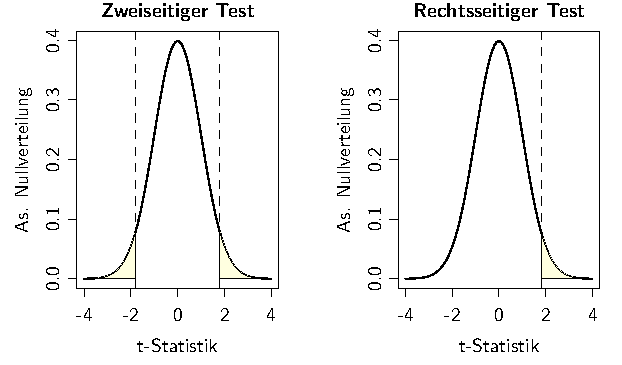
\includegraphics{Resources/Plots/pVal-1} \end{center}
\normalsize
\end{frame}

\begin{frame}{Rezept}
\protect\hypertarget{rezept}{}
Allgemein geht man beim \alert{Hypothesentesten} wie folgt vor:

\begin{enumerate}
\tightlist
\item
  Wähle ein \alert{Signifikanzniveau $\alpha$} (häufig: \(\alpha=5\%\)).
\item
  Finde eine \alert{Teststatistik $T$} mit asymptotischer Verteilung
  \(T\overset{d}{\longrightarrow}\xi\) unter \(\mathbb{H}_0\).
\item
  Setze den asymptotischen \alert{kritischen Wert $c$} so, dass
  \(1-G(c)=\alpha\), wobei \(G\) die Verteilungsfunktion von \(\xi\)
  ist.
\item
  Berechne den (asymptotischen) \alert{$p$-Wert} \(p=1-G(T)\).
\item
  \alert{Lehne $\mathbb{H}_0$ ab}, wenn \(T>c\) oder, äquivalent dazu,
  \(p<\alpha\).
\item
  \alert{Akzeptiere $\mathbb{H}_0$}, wenn \(T\leq c\) oder, äquivalent
  dazu, \(p\geq\alpha\).
\item
  Berichte den \alert{$p$-Wert} als Zusammenfassung der Evidenz
  betreffend \(\mathbb{H}_0\) und \(\mathbb{H}_1\).
\end{enumerate}
\end{frame}

\begin{frame}{Überblick}
\protect\hypertarget{uxfcberblick-19}{}
\begin{itemize}
\tightlist
\item
  Wiederholung Testtheorie
\item
  \textbf{Bedingte Homoskedastie}
\item
  Bedingte Heteroskedastie
\item
  Hypothesentests
\item
  Konfidenzintervalle
\end{itemize}
\end{frame}

\begin{frame}{}
\protect\hypertarget{section-6}{}
\begin{itemize}
\tightlist
\item
  Inferenz befasst sich mit (statistisch abgesicherten)
  \alert{Rückschlüssen von den Daten auf die Wirklichkeit.}
\item
  Wir wissen bereits aus Theorem~\ref{thm:KQ AN}, dass \[
  \sqrt{n}\big(\widehat{\vbeta}-\vbeta\big)\overset{d}{\longrightarrow}N(\vzero, \mV_{\vbeta})
  \] für
  \(\mV_{\vbeta}=\mQ^{-1}_{XX^\prime}\mOmega\mQ^{-1}_{XX^\prime}\).
\item
  Um Rückschlüsse aus den Daten für das wahre \(\vbeta\) gewinnen zu
  können, müssen wir nur noch das \alert{unbekannte} \(\mV_{\vbeta}\)
  schätzen.
\item
  \alert{Wie} \(\mV_{\beta}\) geschätzt werden kann, hängt davon ab, ob
  bedingte Homoskedastie oder bedingte Heteroskedastie vorliegt\ldots{}
\end{itemize}
\end{frame}

\begin{frame}{Bedingte Homoskedastie}
\protect\hypertarget{bedingte-homoskedastie}{}
\begin{itemize}
\tightlist
\item
  Am einfachsten wird Inferenz unter \alert{bedingter Homoskedastie},
  d.h.~wenn \(\E[e^2\mid X]=\sigma^2\) (siehe Annahme
  \ref{ass:cond hom}).
\item
  Dann gilt nämlich: \begin{eqnarray*}
  \mOmega &\overset{\eqref{eq:Omega}}{=}&\E[XX^\prime e^2]\\
  &\overset{\eqref{eq:GIE}}{=}& \E\big[\E(XX^\prime e^2\mid X)\big]\\
  &\overset{\eqref{eq:pull out}}{=}& \E\big[XX^\prime \E( e^2\mid X)\big]\\
  &=& \sigma^2\E[XX^\prime]=\sigma^2\mQ_{XX^\prime}.
  \end{eqnarray*}
\item
  Somit \alert{vereinfacht} sich die asymptotische Varianz aus Theorem
  \ref{thm:KQ AN} zu \[
  \mV_{\vbeta} = \mQ_{XX^\prime}^{-1} \mathcolor{blue}{\mOmega} \mQ_{XX^\prime}^{-1} =  \mQ_{XX^\prime}^{-1}\mathcolor{blue}{\sigma^2} \underbrace{\mathcolor{blue}{\mQ_{XX^\prime}} \mQ_{XX^\prime}^{-1}}_{=\mI}=\sigma^2 \mQ_{XX^\prime}^{-1}.
  \]
\item
  \alert{Aufgabe:} Schätze \(\sigma^2\) und \(\mQ_{XX^\prime}^{-1}\).
\end{itemize}
\end{frame}

\begin{frame}{Schätzer von \(\mQ_{XX^\prime}^{-1}\) und \(\sigma^2\)}
\protect\hypertarget{schuxe4tzer-von-mq_xxprime-1-und-sigma2}{}
\begin{itemize}
\tightlist
\item
  \(\mQ_{XX^\prime}^{-1}\): Direkt aus \eqref{eq:convXX} zu schätzen.
\item
  \(\sigma^2=\E[e^2\mid X]\): Erwartungswert auf Gleichung anwenden
  liefert
  \(\sigma^2=\E[\sigma^2]=\E[\E(e^2\mid X)]\overset{\eqref{eq:GIE}}{=}\E[e^2]\),
  was Stichprobenmittel
  \(\widehat{\sigma}^2 = \frac{1}{n}\widehat{\ve}^\prime\widehat{\ve}\)
  als Schätzer nahelegt.
\item
  \alert{Warum?} \begin{eqnarray*}
  \widehat{\sigma}^2 &=& \frac{1}{n}\widehat{\ve}^\prime\widehat{\ve}\\
  &\overset{\eqref{eq:e hat why}}{=}& \frac{1}{n}(\mM\mY)^\prime(\mM\mY)\\
  &\overset{\text{Prop. }\zref{S-rules2}.\zref{S-it:20.4}}{=}& \frac{1}{n}\mY^\prime\mM^\prime\mM\mY\\
  &\overset{\text{Thm.}\ \ref{thm:Eig M}}{=}& \frac{1}{n}\mY^\prime\mM\mY\\
  &=& \frac{1}{n}(\mX\vbeta+\ve)^\prime\mM(\mX\vbeta+\ve)\\
  &\overset{\mM\mX=\vzero}{=}& \frac{1}{n}\ve^\prime\mM\ve\\
  &=& \frac{1}{n}\ve^\prime(\mI-\mP)\ve.
  \end{eqnarray*}
\end{itemize}
\end{frame}

\begin{frame}{Konsistenz von \(\widehat{\sigma}^2\)}
\protect\hypertarget{konsistenz-von-widehatsigma2}{}
\begin{itemize}
\tightlist
\item
  Die Definition von \(\mP\) ausnutzend, erhalten wir damit:
  \begin{equation*}
  \widehat{\sigma}^2 = \frac{\ve^\prime\ve}{n} - \frac{\ve^\prime\mX}{n} \Big(\frac{\mX^\prime\mX}{n}\Big)^{-1}  \frac{\mX^\prime\ve}{n}
  \end{equation*}
\item
  Das ist eine \alert{stetige Funktion} in drei Argumenten:
  \begin{align*}
  \Big(\frac{\mX^\prime\mX}{n}\Big)^{-1} &\overset{\Pr}{\longrightarrow}\mQ_{XX^\prime}^{-1}&&(\text{siehe } \eqref{eq:convXX}),\\
  \frac{\ve^\prime\mX}{n} &\overset{\Pr}{\longrightarrow}\vzero &&(\text{siehe } \eqref{eq:cons2}),\\
  \frac{\ve^\prime\ve}{n} &\overset{\Pr}{\longrightarrow}\sigma^2&&(\text{Warum?}).
  \end{align*}
\item
  Das CMT 1 impliziert deshalb: \[
  \widehat{\sigma}^2\overset{\Pr}{\longrightarrow}\sigma^2.
  \]
\end{itemize}
\end{frame}

\begin{frame}{Zusammenfassung}
\protect\hypertarget{zusammenfassung-1}{}
\begin{itemize}
\tightlist
\item
  Wir schreiben das Obige nochmal kompakt auf:
\end{itemize}

\thmn\label{thm:KQ under cond homo} Im linearen Projektionsmodell gilt
unter den Annahmen \ref{ass:1}, \ref{ass:iid} und \ref{ass:cond hom},
dass \begin{align*}
  \widehat{\sigma}^2&\overset{\Pr}{\longrightarrow}\sigma^2,\\
  \widehat{\mQ}_{XX^\prime}^{-1}:=\Big(\frac{\mX^\prime\mX}{n}\Big)^{-1}&\overset{\Pr}{\longrightarrow}\mQ_{XX^\prime}^{-1},\\ \widehat{\mV}_{\vbeta}^{0}:=\widehat{\sigma}^2\Big(\frac{\mX^\prime\mX}{n}\Big)^{-1}& \overset{\Pr}{\longrightarrow}\sigma^2\mQ_{XX^\prime}^{-1}=:\mV_{\vbeta}^{0}.
\end{align*} \endthmn
\end{frame}

\begin{frame}{Anwendung}
\protect\hypertarget{anwendung}{}
\begin{itemize}
\tightlist
\item
  \alert{Wofür} das Ganze?
\item
  Theoreme \ref{thm:KQ AN} und \ref{thm:KQ under cond homo} implizieren
  unter \alert{bedingter Homoskedastie} (zusammen mit dem Satz von
  Slutzky) \[
  \big(\widehat{\mV}_{\vbeta}^{0}\big)^{-1/2}\sqrt{n}\big(\widehat{\vbeta} - \vbeta\big) \overset{d}{\longrightarrow} \big(\mV_{\vbeta}^{0}\big)^{-1/2} N(\vzero, \mV_{\vbeta}^{0}).
  \]
\item
  Ähnliche Argumente wie in Schritt 3/3 des Beweises von Theorem
  \ref{thm:KQ AN} liefern: \begin{align*}
  \big(\mV_{\vbeta}^{0}\big)^{-1/2} N(\vzero, \mV_{\vbeta}^{0})&\overset{d}{=}N\Big(\vzero, \big(\mV_{\vbeta}^{0}\big)^{-1/2}\big(\mV_{\vbeta}^{0}\big)^{1/2}\big(\mV_{\vbeta}^{0}\big)^{1/2}\big(\mV_{\vbeta}^{0}\big)^{-1/2}\Big)\\
  &=N(\vzero,\mI).
  \end{align*}
\item
  Also: \begin{equation}\label{eq:beta hat cond homo}
  \boxed{\ \big(\widehat{\mV}_{\vbeta}^{0}\big)^{-1/2}\sqrt{n}\big(\widehat{\vbeta} - \vbeta\big) \overset{d}{\longrightarrow}N(\vzero, \mI).\ } 
  \end{equation}
\item
  Dieses Resultat können wir für Inferenzzwecke nutzen, aber bedingte
  Homoskedastie ist sehr speziell.
\item
  Daher schauen wir uns Inferenz direkt für den allgemeineren Fall der
  \alert{bedingten Heteroskedastie} an.
\end{itemize}
\end{frame}

\begin{frame}{Überblick}
\protect\hypertarget{uxfcberblick-20}{}
\begin{itemize}
\tightlist
\item
  Wiederholung Testtheorie
\item
  Bedingte Homoskedastie
\item
  \textbf{Bedingte Heteroskedastie}
\item
  Hypothesentests
\item
  Konfidenzintervalle
\end{itemize}
\end{frame}

\begin{frame}{Bedingte Heteroskedastie}
\protect\hypertarget{bedingte-heteroskedastie}{}
\begin{itemize}
\tightlist
\item
  Die Annahme bedingter Homoskedastie ist häufig \alert{nicht erfüllt}.
\end{itemize}

\xmpl[Heteroskedastie ist ganz natürlich]

\begin{itemize}
\tightlist
\item
  Betrachte das \alert{lineare bedingter Erwartungswertmodell} mit
  \alert{binärer} abhängiger Variable \(Y\in\{0,1\}\):
  \begin{equation}\label{eq:toy model}
  Y=X^\prime\vbeta+e,\qquad \E[e\mid X]=0.
  \end{equation}
\item
  Dann gilt \begin{eqnarray*}
  \E[e^2\mid X] &\overset{\E[e\mid X]=0}{=}& \Var(e\mid X) \\
  &\overset{\eqref{eq:toy model}}{=}& \Var(Y\mid X) \\
  &\overset{\text{Thm. }\ref{thm:bed mom}}{=}& \E[Y^2\mid X] - \big(\E[Y\mid X]\big)^2 \\
  &\overset{Y\in\{0,1\}}{=}& \E[Y\mid X] \big(1 - \E[Y\mid X]\big)\\
  &\overset{\eqref{eq:toy model}}{=}& X^\prime\vbeta(1-X^\prime\vbeta).
  \end{eqnarray*}
\item
  Wir haben also \alert{bedingte Heteroskedastizität:} Die bedingte
  Varianz variiert mit \(X\)!
\end{itemize}

\endxmpl
\end{frame}

\begin{frame}{Bedingte Heteroskedastie}
\protect\hypertarget{bedingte-heteroskedastie-1}{}
\begin{itemize}
\tightlist
\item
  Weil bedingte Heteroskedastizität die Regel ist, wird die
  Approximation in \eqref{eq:beta hat cond homo} dann
  \alert{nicht stimmen}, genau so wie alles, was darauf aufbaut\ldots{}

  \begin{itemize}
  \tightlist
  \item
    Hypothesentests
  \item
    Konfidenzintervalle
  \end{itemize}
\item
  Im allgemeinen Fall (siehe Theorem \ref{thm:KQ AN}) ist
  \(\mV_{\vbeta}=\mQ^{-1}_{XX^\prime}\mOmega\mQ^{-1}_{XX^\prime}\) und
  wir müssen noch \[
  \mOmega\overset{\eqref{eq:Omega}}{=}\E[XX^\prime e^2]
  \] schätzen.
\item
  Was läge da näher als \begin{align}
  \widehat{\mOmega} &= \frac{1}{n}\sum_{i=1}^{n}\widehat{e}_i^2X_i X_i^\prime,\label{eq:Omega hat}\\
  \widehat{\mV}_{\vbeta}^{\text{HC0}} &= \widehat{\mQ}^{-1}_{XX^\prime}\widehat{\mOmega}\widehat{\mQ}^{-1}_{XX^\prime}.
  \end{align}
\end{itemize}
\end{frame}

\begin{frame}{Konsistenz von \(\widehat{\mOmega}\) und
\(\widehat{\mV}_{\vbeta}^{\text{HC0}}\)}
\protect\hypertarget{konsistenz-von-widehatmomega-und-widehatmv_vbetatexthc0}{}
\thmn[Hansen (2022, Theorem 7.6)]\label{thm:KQ under cond hetero} Im
linearen Projektionsmodell gilt unter den Annahmen \ref{ass:iid} und
\ref{ass:1 ex}, dass \[
  \widehat{\mOmega}\overset{\Pr}{\longrightarrow}\mOmega\qquad\text{und}\qquad \widehat{\mV}_{\vbeta}^{\text{HC0}}\overset{\Pr}{\longrightarrow}\mV_{\vbeta}.
\] \endthmn

\begin{itemize}
\tightlist
\item
  Aus offensichtlichen Gründen wird
  \(\widehat{\mV}_{\vbeta}^{\text{HC0}}\)
  \hil{Heteroskedastie-konsistenter Kovarianz-Matrix Schätzer} genannt.
\item
  Es gibt eine Reihe von \alert{Varianten} von
  \(\widehat{\mV}_{\vbeta}^{\text{HC0}}\), bezeichnet
  \(\widehat{\mV}_{\vbeta}^{\text{HC1}},\ldots,\widehat{\mV}_{\vbeta}^{\text{HC5}}\).

  \begin{itemize}
  \tightlist
  \item
    Z.B.~ersetzt \(\widehat{\mV}_{\vbeta}^{\text{HC1}}\) in
    \eqref{eq:Omega hat} die Residuen \(\widehat{e}_i^2\) durch
    \(n/(n-k)\widehat{e}_i^2\).
  \end{itemize}
\item
  Unter den Annahmen von Theorem~\ref{thm:KQ under cond hetero}:
  \begin{equation}\label{eq:beta hat cond hetero}
  \boxed{\ \big(\widehat{\mV}_{\vbeta}^{\text{HC0}}\big)^{-1/2}\sqrt{n}\big(\widehat{\vbeta} - \vbeta\big) \overset{d}{\longrightarrow}N(\vzero, \mI).\ } 
  \end{equation}
\end{itemize}
\end{frame}

\begin{frame}{Überblick}
\protect\hypertarget{uxfcberblick-21}{}
\begin{itemize}
\tightlist
\item
  Wiederholung Testtheorie
\item
  Bedingte Homoskedastie
\item
  Bedingte Heteroskedastie
\item
  \textbf{Hypothesentests}
\item
  Konfidenzintervalle
\end{itemize}
\end{frame}

\begin{frame}{\(t\)-Test}
\protect\hypertarget{t-test}{}
\begin{itemize}
\tightlist
\item
  Im Rest dieses Kapitels formulieren wir alle Resultate basierend auf
  dem \alert{allgemeinen Ergebnis} \eqref{eq:beta hat cond hetero}.

  \begin{itemize}
  \tightlist
  \item
    Die Resultate für den \alert{Spezialfall} der bedingten
    Homoskedastie erhält man durch ersetzen von
    \(\widehat{\mV}_{\vbeta}^{\text{HC0}}\) durch
    \(\widehat{\mV}_{\vbeta}^{0}\); vgl.~\eqref{eq:beta hat cond homo}.
  \end{itemize}
\item
  Wir fangen mit dem einfachsten Test einer
  \alert{einzigen linearen Restriktion} an: \[
  \boxed{\ \mathbb{H}_0\colon \va^\prime\vbeta=r,\ }
  \] wobei \(\underset{(k\times 1)}{\va}\) ein bekannter Vektor ist und
  \(r\) ein bekannter Skalar.

  \begin{itemize}
  \tightlist
  \item
    Häufigster Fall: Test auf \hil{Signifikanz} der \(i\)-ten Variable,
    d.h.~\(\mathbb{H}_0\colon \beta_i=0\).
  \item
    Wenn wir \(\mathbb{H}_0\colon \beta_i=0\) ablehnen können, dann ist
    \(X_i\) \hil{signifikant}.
  \end{itemize}
\end{itemize}
\end{frame}

\begin{frame}{\(t\)-Test}
\protect\hypertarget{t-test-1}{}
\framesubtitle{Die Konstruktion}

\begin{itemize}
\tightlist
\item
  Das CMT 2 und Theorem \ref{thm:KQ AN} implizieren \[
  \sqrt{n}\big(\va^\prime\widehat{\vbeta}- \va^\prime\vbeta\big)\overset{d}{\longrightarrow}\va^\prime N(\vzero, \mV_{\vbeta})\overset{d}{=}N(\va^\prime\vzero, \va^\prime\mV_{\vbeta}\va)=N(0, \va^\prime\mV_{\vbeta}\va).
  \]
\item
  Unter \(\mathbb{H}_0\colon\va^\prime\vbeta=r\) gilt dann
  \begin{equation}\label{eq:h2}
  \sqrt{n}\big(\va^\prime\widehat{\vbeta}- r\big)\overset{d}{\longrightarrow}N(0, \va^\prime\mV_{\vbeta}\va).
  \end{equation}
\item
  Das CMT 1 und Theorem \ref{thm:KQ under cond hetero} implizieren
  \begin{equation}\label{eq:h3}
  \va^\prime\widehat{\mV}_{\vbeta}^{\text{HC0}}\va \overset{\Pr}{\longrightarrow}\va^\prime\mV_{\vbeta}\va.
  \end{equation}
\item
  Aus dem Satz von Slutzky zusammen mit \eqref{eq:h2}--\eqref{eq:h3}
  folgt für die \hil{$t$-Statistik} \[
  t=\frac{\va^\prime\widehat{\vbeta}- r}{\sqrt{\va^\prime\widehat{\mV}_{\vbeta}^{\text{HC0}}\va/n}}=\frac{\sqrt{n}(\va^\prime\widehat{\vbeta}- r)}{\sqrt{\va^\prime\widehat{\mV}_{\vbeta}^{\text{HC0}}\va}}\overset{d}{\longrightarrow}\frac{N(0,\va^\prime\mV_{\vbeta}\va)}{\sqrt{\va^\prime\mV_{\vbeta}\va}}=N(0,1),
  \] falls \(\va^\prime\mV_{\vbeta}\va>0\).
\end{itemize}
\end{frame}

\begin{frame}{\(t\)-Test}
\protect\hypertarget{t-test-2}{}
\framesubtitle{Zusammenfassung}

\begin{itemize}
\tightlist
\item
  Wir sammeln Obiges wieder in einem Theorem:\medskip
\end{itemize}

\thmn[\hil{$t$-Test}]\label{thm:t Test} Gelten die Annahmen von Theorem
\ref{thm:KQ under cond hetero}. Dann gilt unter
\(\mathbb{H}_0\colon \va^\prime\vbeta=r\) falls
\(\va^\prime\mV_{\vbeta}\va>0\), dass
\begin{equation}\label{eq:t statistic}
  t=\frac{\va^\prime\widehat{\vbeta}- r}{\sqrt{\va^\prime\widehat{\mV}_{\vbeta}^{\text{HC0}}\va/n}}\overset{d}{\longrightarrow}N(0,1).
\end{equation} Im speziellen Fall, dass \(\mathbb{H}_0\colon\beta_i=0\),
gilt \[
  \boxed{\ t=\frac{\widehat{\beta}_i}{\sqrt{\big(\widehat{\mV}_{\vbeta}^{\text{HC0}}\big)_{ii}/n}}\overset{d}{\longrightarrow}N(0,1),\ }
\] wobei \(\big(\widehat{\mV}_{\vbeta}^{\text{HC0}}\big)_{ii}\) das
\(i\)-te Diagonalelement der Matrix
\(\widehat{\mV}_{\vbeta}^{\text{HC0}}\) bezeichnet.

Wir bezeichnen
\(\sqrt{\big(\widehat{\mV}_{\vbeta}^{\text{HC0}}\big)_{ii}/n}\) als den
\hil{Standardfehler} des Schätzers \(\widehat{\beta}_i\). \endthmn
\end{frame}

\begin{frame}{\(t\)-Test}
\protect\hypertarget{t-test-3}{}
\framesubtitle{Anwendung}

\begin{itemize}
\tightlist
\item
  Aus Theorem \ref{thm:t Test} ergibt sich folgender
  \alert{Test zum asymptotischen Signifikanzniveau $\alpha$} der
  Hypothese \(\mathbb{H}_0\colon \va^\prime\vbeta=r\):
  \begin{equation}\label{eq:t Test}
  \boxed{\ \text{Verwirf }\mathbb{H}_0\text{, falls }\quad T=|t|>\Phi^{-1}(1-\alpha/2).\ }
  \end{equation}
\item
  Der (asymptotische) \alert{$p$-Wert} ist (siehe Beispiel
  \ref{ex:p val}) \[
  p=2\big[1-\Phi(|t|)\big].
  \]
\item
  Für die konkrete Alternative
  \(\mathbb{H}_1\colon\va^\prime\vbeta=r_1\neq r\), lässt sich die
  \alert{Macht} berechnen als \[
  \Pr\big\{\text{Verwirf}\ \mathbb{H}_0\mid \mathbb{H}_1\ \text{ist wahr}\big\}=\Pr\big\{|t|>\Phi^{-1}(1-\alpha/2)\mid \va^\prime\vbeta=r_1\big\}.
  \]
\item
  Für \(n\to\infty\) lässt sich hierfür ein Ausdruck finden\ldots{}
\end{itemize}
\end{frame}

\begin{frame}{\(t\)-Test in \R}
\protect\hypertarget{t-test-in}{}
\xmpl[Card (1995)]\label{ex:Card1}

\begin{itemize}
\tightlist
\item
  Wir erweitern die Lohnregression von Card (1995) um weitere
  Regressoren: \begin{align*}
  experience &= \alert{age - educ - 6}\ (exper), \\
  black &= \text{\alert{Indikatorvariable fuer Hautfarbe}}\ (black),\\
  south &= \text{\alert{Indikatorvariable fuer Suedstaaten}}\ (reg76r),\\
  urban &= \text{\alert{Indikatorvariable fuer Standard Metropolitan Statistical Area}}\ (smsa76r).
  \end{align*}
\item
  Wir betrachten dann die KQ Regression: \begin{multline}
  \log(wage) =  \beta_0+ \beta_1\cdot educ + \beta_2\cdot exper + \beta_3\cdot(exper/100)^2 + \\
   \beta_4\cdot black + \beta_5\cdot south + \beta_6\cdot urban + e. \label{eq:Card1}
  \end{multline}
\item
  Alle Regressoren sind \alert{signifikante} Prädiktoren des Gehalts,
  d.h.~wir können \(\mathbb{H}_0\colon\beta_i=0\) ablehnen.

  \begin{itemize}
  \tightlist
  \item
    \alert{Achtung:} Heißt nur signifikant im
    \alert{linearen Projektionsmodell}, ob die Regressoren auch
    signifikant im \alert{wahren DGP} sind, steht auf einem anderen
    Blatt!
  \end{itemize}
\end{itemize}

\endxmpl
\end{frame}

\begin{frame}[fragile,allowframebreaks]{\(t\)-Test im \R Beispiel}
\protect\hypertarget{t-test-im-beispiel}{}
\footnotesize

\begin{Shaded}
\begin{Highlighting}[]
\NormalTok{card}\SpecialCharTok{$}\NormalTok{exper      }\OtherTok{\textless{}{-}}\NormalTok{ card}\SpecialCharTok{$}\NormalTok{age76 }\SpecialCharTok{{-}}\NormalTok{ card}\SpecialCharTok{$}\NormalTok{ed76 }\SpecialCharTok{{-}} \DecValTok{6}         \CommentTok{\# add experience variable}
\NormalTok{card            }\OtherTok{\textless{}{-}}\NormalTok{ card[}\FunctionTok{is.na}\NormalTok{(card}\SpecialCharTok{$}\NormalTok{lwage76)}\SpecialCharTok{==}\ConstantTok{FALSE}\NormalTok{, ] }\CommentTok{\# remove NAs}
\NormalTok{KQ              }\OtherTok{\textless{}{-}} \FunctionTok{lm}\NormalTok{(lwage76 }\SpecialCharTok{\textasciitilde{}}\NormalTok{ ed76 }\SpecialCharTok{+}\NormalTok{ exper }\SpecialCharTok{+} \FunctionTok{I}\NormalTok{(exper}\SpecialCharTok{\^{}}\DecValTok{2}\SpecialCharTok{/}\DecValTok{100}\NormalTok{) }\SpecialCharTok{+}\NormalTok{ black }\SpecialCharTok{+} 
\NormalTok{                        reg76r }\SpecialCharTok{+}\NormalTok{ smsa76r, }\AttributeTok{data=}\NormalTok{card)}
\FunctionTok{summary}\NormalTok{( KQ )  }\CommentTok{\# only shows homoskedasticity{-}only standard errors (s.e.s)}
\end{Highlighting}
\end{Shaded}

\begin{verbatim}
## 
## Call:
## lm(formula = lwage76 ~ ed76 + exper + I(exper^2/100) + black + 
##     reg76r + smsa76r, data = card)
## 
## Residuals:
##     Min      1Q  Median      3Q     Max 
## -1.5930 -0.2232  0.0189  0.2422  1.3319 
## 
## Coefficients:
##                Estimate Std. Error t value Pr(>|t|)    
## (Intercept)     4.73366    0.06760   70.02  < 2e-16 ***
## ed76            0.07401    0.00351   21.11  < 2e-16 ***
## exper           0.08360    0.00665   12.57  < 2e-16 ***
## I(exper^2/100) -0.22409    0.03178   -7.05  2.2e-12 ***
## black          -0.18963    0.01763  -10.76  < 2e-16 ***
## reg76r         -0.12486    0.01512   -8.26  < 2e-16 ***
## smsa76r         0.16142    0.01557   10.37  < 2e-16 ***
## ---
## Signif. codes:  0 '***' 0.001 '**' 0.01 '*' 0.05 '.' 0.1 ' ' 1
## 
## Residual standard error: 0.374 on 3003 degrees of freedom
## Multiple R-squared:  0.291,  Adjusted R-squared:  0.289 
## F-statistic:  205 on 6 and 3003 DF,  p-value: <2e-16
\end{verbatim}

\begin{Shaded}
\begin{Highlighting}[]
\FunctionTok{library}\NormalTok{(sandwich)}
\FunctionTok{library}\NormalTok{(lmtest)}
\NormalTok{teststatsRobust }\OtherTok{\textless{}{-}} \FunctionTok{coeftest}\NormalTok{(KQ, }\AttributeTok{df =} \ConstantTok{Inf}\NormalTok{, }\AttributeTok{vcov =} \FunctionTok{vcovHC}\NormalTok{(KQ, }\AttributeTok{type=}\StringTok{"HC0"}\NormalTok{))  }\CommentTok{\# HC{-}consistent s.e.s}
\NormalTok{teststatsRobust}
\end{Highlighting}
\end{Shaded}

\begin{verbatim}
## 
## z test of coefficients:
## 
##                Estimate Std. Error z value Pr(>|z|)    
## (Intercept)     4.73366    0.07008   67.55  < 2e-16 ***
## ed76            0.07401    0.00364   20.34  < 2e-16 ***
## exper           0.08360    0.00672   12.43  < 2e-16 ***
## I(exper^2/100) -0.22409    0.03177   -7.05  1.8e-12 ***
## black          -0.18963    0.01741  -10.89  < 2e-16 ***
## reg76r         -0.12486    0.01533   -8.14  3.8e-16 ***
## smsa76r         0.16142    0.01516   10.65  < 2e-16 ***
## ---
## Signif. codes:  0 '***' 0.001 '**' 0.01 '*' 0.05 '.' 0.1 ' ' 1
\end{verbatim}

\normalsize
\end{frame}

\begin{frame}{Wald Test}
\protect\hypertarget{wald-test}{}
\begin{itemize}
\tightlist
\item
  Oft ist es von Interesse, \alert{mehrere Restriktionen} gleichzeitig
  zu testen.
\item
  Deshalb betrachten wir nun \[
  \boxed{\ \mathbb{H}_0\colon \mR^\prime\vbeta=\vr,\ }
  \] wobei \(\underset{(k\times q)}{\mR}\) vollen Spaltenrang \(q\) hat
  (d.h.~wir testen \alert{keine linear redundanten} Hypothesen) und
  \(\underset{(q\times 1)}{\vr}\) ein bekannter Wert ist.
\item
  Z.B.~können wir die \alert{gemeinsame Signifikanz} aller Regressoren
  testen, d.h. \[
  \mathbb{H}_0\colon \beta_1=\ldots=\beta_k=0.
  \]

  \begin{itemize}
  \tightlist
  \item
    Hier: \(\mR=\mI_{k}\) und \(\vr=\vzero\).
  \end{itemize}
\end{itemize}
\end{frame}

\begin{frame}{Wald Test}
\protect\hypertarget{wald-test-1}{}
\framesubtitle{Die Konstruktion}

\begin{itemize}
\tightlist
\item
  Das CMT 2 und Theorem \ref{thm:KQ AN} implizieren \[
  \sqrt{n}\big(\mR^\prime\widehat{\vbeta}- \mR^\prime\vbeta\big)\overset{d}{\longrightarrow}\mR^\prime N(\vzero, \mV_{\vbeta})\overset{d}{=}N(\mR^\prime\vzero, \mR^\prime\mV_{\vbeta}\mR)=N(\vzero, \mR^\prime\mV_{\vbeta}\mR).
  \]
\item
  Unter \(\mathbb{H}_0\colon\mR^\prime\vbeta=\vr\) gilt dann
  \begin{equation}\label{eq:h4}
  \sqrt{n}\big(\mR^\prime\widehat{\vbeta}- \vr\big)\overset{d}{\longrightarrow}N(\vzero, \mR^\prime\mV_{\vbeta}\mR).
  \end{equation}
\item
  Das CMT 1 und Theorem \ref{thm:KQ under cond hetero} implizieren
  \begin{equation}\label{eq:h5}
  \mR^\prime\widehat{\mV}_{\vbeta}^{\text{HC0}}\mR \overset{\Pr}{\longrightarrow}\mR^\prime\mV_{\vbeta}\mR.
  \end{equation}
\item
  Aus dem Satz von Slutzky zusammen mit \eqref{eq:h4}--\eqref{eq:h5}
  folgt \begin{equation}\label{eq:h6}
  \big(\mR^\prime\widehat{\mV}_{\vbeta}^{\text{HC0}}\mR\big)^{-1/2}\sqrt{n}\big(\mR^\prime\widehat{\vbeta}- \vr\big)\overset{d}{\longrightarrow}N(\vzero,\mI).
  \end{equation}
\end{itemize}
\end{frame}

\begin{frame}{Wald Test}
\protect\hypertarget{wald-test-2}{}
\framesubtitle{Die Konstruktion}

\begin{itemize}
\tightlist
\item
  Das CMT 2 angewandt auf \eqref{eq:h6} liefert \[
  \sqrt{n}\big(\mR^\prime\widehat{\vbeta}- \vr\big)^\prime\Big[\big(\mR^\prime\widehat{\mV}_{\vbeta}^{\text{HC0}}\mR\big)^{-1/2}\Big]^\prime \big(\mR^\prime\widehat{\mV}_{\vbeta}^{\text{HC0}}\mR\big)^{-1/2}\sqrt{n}\big(\mR^\prime\widehat{\vbeta}- \vr\big)\overset{d}{\longrightarrow}\mZ^\prime\mZ,
  \] wobei \(\mZ\sim N(\vzero,\mI)\).
\item
  Per Definition der \(\chi^2\)-Verteilung gilt
  \(\mZ^\prime\mZ\sim \chi^2_q\), als Summe \(q\) unabhängiger
  quadrierter Normalverteilungen.
\item
  Somit gilt für die \hil{Wald Statistik} \[
  W=n (\mR^\prime\widehat{\vbeta}- \vr)^\prime (\mR^\prime\widehat{\mV}_{\vbeta}^{\text{HC0}}\mR)^{-1}(\mR^\prime\widehat{\vbeta}- \vr)\overset{d}{\longrightarrow}\chi^2_q,
  \] falls \(\mR^\prime\mV_{\vbeta}\mR>0\) (also p.d.).
\end{itemize}
\end{frame}

\begin{frame}{Wald Test}
\protect\hypertarget{wald-test-3}{}
\framesubtitle{Zusammenfassung und Anwendung}

\begin{itemize}
\tightlist
\item
  Wir sammeln Obiges wieder in einem Theorem:\medskip
\end{itemize}

\thmn[\hil{Wald Test}]\label{thm:Wald Test} Gelten die Annahmen von
Theorem~\ref{thm:KQ under cond hetero}. Dann gilt unter
\(\mathbb{H}_0\colon \mR^\prime\vbeta=\vr\) falls
\(\mR^\prime\mV_{\vbeta}\mR>0\), dass \[
  \boxed{\ W=n (\mR^\prime\widehat{\vbeta}- \vr)^\prime (\mR^\prime\widehat{\mV}_{\vbeta}^{\text{HC0}}\mR)^{-1}(\mR^\prime\widehat{\vbeta}- \vr)\overset{d}{\longrightarrow}\chi^2_q.\ }
\] \endthmn

\begin{itemize}
\tightlist
\item
  Aus Theorem \ref{thm:Wald Test} ergibt sich folgender
  \alert{Test zum asymptotischen Signifikanzniveau $\alpha$} der
  Hypothese \(\mathbb{H}_0\colon \mR^\prime\vbeta=\vr\): \[
  \boxed{\ \text{Verwirf }\mathbb{H}_0\text{, falls }\quad W>\chi^{2,-1}_q(1-\alpha).\ }
  \]
\item
  Der (asymptotische) \alert{$p$-Wert} ist \[
  p=1-\chi_{q}^{2}(W),
  \] wobei \(\chi_{q}^{2}(\cdot)\) die Verteilungsfunktion einer
  \(\chi_q^2\)-Verteilung ist.
\end{itemize}
\end{frame}

\begin{frame}[fragile]{Wald Test in \R}
\protect\hypertarget{wald-test-in}{}
\xmpl[Card (1995)]

\begin{itemize}
\tightlist
\item
  Wir testen die Hypothese
  \(\mathbb{H}_0\colon \beta_1=\ldots=\beta_6=0\) im Modell
  \eqref{eq:Card1}.

  \begin{itemize}
  \tightlist
  \item
    Warum testen wir nicht auch noch \(\beta_0=0\)?
  \end{itemize}
\item
  Nicht weiter erstaunlich, dass die Prädiktoren auch
  \alert{gemeinsam signifikant} sind.
\end{itemize}

\endxmpl

\footnotesize

\begin{Shaded}
\begin{Highlighting}[]
\FunctionTok{waldtest}\NormalTok{(KQ, }\DecValTok{1}\SpecialCharTok{:}\DecValTok{6}\NormalTok{, }\AttributeTok{vcov =} \FunctionTok{vcovHC}\NormalTok{(KQ, }\AttributeTok{type=}\StringTok{"HC0"}\NormalTok{), }\AttributeTok{test =} \StringTok{"Chisq"}\NormalTok{)}
\end{Highlighting}
\end{Shaded}

\begin{verbatim}
## Wald test
## 
## Model 1: lwage76 ~ ed76 + exper + I(exper^2/100) + black + reg76r + smsa76r
## Model 2: lwage76 ~ 1
##   Res.Df Df Chisq Pr(>Chisq)    
## 1   3003                        
## 2   3009 -6  1309     <2e-16 ***
## ---
## Signif. codes:  0 '***' 0.001 '**' 0.01 '*' 0.05 '.' 0.1 ' ' 1
\end{verbatim}

\normalsize
\end{frame}

\begin{frame}{Überblick}
\protect\hypertarget{uxfcberblick-22}{}
\begin{itemize}
\tightlist
\item
  Wiederholung Testtheorie
\item
  Bedingte Homoskedastie
\item
  Bedingte Heteroskedastie
\item
  Hypothesentests
\item
  \textbf{Konfidenzintervalle}
\end{itemize}
\end{frame}

\begin{frame}{Konfidenzintervalle}
\protect\hypertarget{konfidenzintervalle}{}
\begin{itemize}
\tightlist
\item
  Natürlich glaubt wegen Schätzunsicherheit keiner daran, dass für einen
  \hil{Punktschätzer} \(\widehat{\vtheta}=\vtheta\) in endlichen
  Stichproben gilt.

  \begin{itemize}
  \tightlist
  \item
    Z.B.~\(\vtheta=\vbeta\) und \(\widehat{\vtheta}=\widehat{\vbeta}\).
  \end{itemize}
\item
  Was wäre, wenn wir anstatt einer Punktschätzung, eine geeignete
  \hil{mengenwertige Schätzung} \(\widehat{C}\) angeben?

  \begin{itemize}
  \tightlist
  \item
    Z.B.~\(\widehat{C}=[\widehat{L},\widehat{U}]\) für \(\beta_i\), was
    wir dann eine \hil{Intervallschätzung} nennen.
  \end{itemize}
\end{itemize}

\defn[Konfidenzintervalle und -regionen]Eine mengenwertige Schätzung
\(\widehat{C}\) mit vorspezifizierter
\hil{Überdeckungswahrscheinlichkeit} \(1-\alpha\) (\(0<\alpha<1\)), so
dass \(\Pr\{\vtheta\in\widehat{C}\}=1-\alpha\), nennen wir ein

\begin{itemize}
  \item \hil{Konfidenzintervall}, wenn $\vtheta$ ein Skalar bzw.
  \item \hil{Konfidenzregion}, wenn $\vtheta$ vektorwertig!
\end{itemize}
\enddefn
\end{frame}

\begin{frame}{Allgemeine Konstruktion}
\protect\hypertarget{allgemeine-konstruktion}{}
\begin{itemize}
\tightlist
\item
  Meist nur \hil{asymptotische Konfidenzintervalle bzw.\ -regionen},
  d.h.~\(\lim_{n\to\infty}\Pr\{\vtheta\in\widehat{C}\}=1-\alpha\).
\item
  Doch wie \alert{konstruieren} wir solche?
\item
  \(\widehat{C}=\mathbb{R}^{q}\) mit Wkt.~\(1-\alpha\) und
  \(\widehat{C}=\emptyset\) mit Wkt.~\(\alpha\) ist eine
  \alert{valide Konfidenzregion}, aber offensichtlich
  \alert{keine gute Wahl}, da im Durchschnitt viel zu groß.
\item
  Eine bessere \alert{Möglichkeit} ist \(\widehat{C}\) zu definieren als
  \begin{equation}\label{eq:Def C}
  \boxed{\ \widehat{C}:=\big\{\vtheta_0\mid \mathbb{H}_0\colon \vtheta=\vtheta_0\ \text{kann z.N.}\ \alpha\ \text{nicht abgelehnt werden}\big\}.\ }
  \end{equation}
\item
  Diese Konstruktion probieren wir nun aus für

  \begin{enumerate}
  \tightlist
  \item
    \(\vtheta=\va^\prime\vbeta\) (für \alert{Konfidenzintervalle}) und
  \item
    \(\vtheta=\mR^\prime\vbeta\) (für \alert{Konfidenzregionen}).
  \end{enumerate}
\end{itemize}
\end{frame}

\begin{frame}{1.~\(\vtheta=\va^\prime\vbeta\)}
\protect\hypertarget{vthetavaprimevbeta}{}
\begin{itemize}
\tightlist
\item
  Angenommen wir interessieren uns für ein \alert{Konfidenzintervall}
  des Parameters \(\va^\prime\vbeta\).

  \begin{itemize}
  \tightlist
  \item
    Z.B.~\(\beta_i\), wenn \(\va\) dem \(i\)-ten Einheitsvektor
    entspricht.
  \end{itemize}
\item
  \eqref{eq:Def C} sagt uns nun, dass \begin{eqnarray}
  \widehat{C} &=& \big\{r\mid \mathbb{H}_0\colon \va^\prime\vbeta=r\ \text{kann z.N.}\ \alpha\ \text{nicht abgelehnt werden}\big\}\notag\\
  &\overset{\eqref{eq:t Test}}{=} & \big\{r\mid |t|\leq\Phi^{-1}(1-\alpha/2)\big\}\label{eq:h7}\\
  &\overset{\eqref{eq:t statistic}}{=}& \bigg\{r\mid -\Phi^{-1}(1-\alpha/2)\leq \frac{\va^\prime\widehat{\vbeta}-r}{\sqrt{\va^\prime\widehat{\mV}_{\vbeta}^{\text{HC0}}\va/n}} \leq\Phi^{-1}(1-\alpha/2)\bigg\}\notag\\
  &=& \Big\{r\mid \va^\prime\widehat{\vbeta}-\Phi^{-1}(1-\alpha/2)\sqrt{\va^\prime\widehat{\mV}_{\vbeta}^{\text{HC0}}\va/n}\leq r \leq\notag\\
  &&\hspace{3cm}\va^\prime\widehat{\vbeta} + \Phi^{-1}(1-\alpha/2)\sqrt{\va^\prime\widehat{\mV}_{\vbeta}^{\text{HC0}}\va/n}\Big\}\notag\\
  &=&\Big[\va^\prime\widehat{\vbeta} \pm \Phi^{-1}(1-\alpha/2)\sqrt{\va^\prime\widehat{\mV}_{\vbeta}^{\text{HC0}}\va/n}\Big].\notag
  \end{eqnarray}
\end{itemize}
\end{frame}

\begin{frame}{1.~\(\vtheta=\va^\prime\vbeta\)}
\protect\hypertarget{vthetavaprimevbeta-1}{}
\thmn\label{thm:conf int t} Unter den Annahmen von Theorem
\ref{thm:t Test} ist \[
  \widehat{C} = \Big[\va^\prime\widehat{\vbeta} \pm \Phi^{-1}(1-\alpha/2)\sqrt{\va^\prime\widehat{\mV}_{\vbeta}^{\text{HC0}}\va/n}\Big]
\] ein asymptotisches \((1-\alpha)\)-Konfidenzintervall für den
Parameter \(\va^\prime\vbeta\).\medskip

Im Spezialfall, dass \(\va^\prime\vbeta=\beta_i\), ist \[
  \boxed{\ \widehat{C} = \Big[\widehat{\beta_i} \pm \Phi^{-1}(1-\alpha/2)\sqrt{\big(\widehat{\mV}_{\vbeta}^{\text{HC0}}\big)_{ii}/n}\Big]\ }
\] ein asymptotisches \((1-\alpha)\)-Konfidenzintervall für \(\beta_i\).
\endthmn

\begin{proof}
Folgt direkt aus \eqref{eq:h7} und Theorem \ref{thm:t Test}.
\end{proof}
\end{frame}

\begin{frame}{1.~\(\vtheta=\va^\prime\vbeta\)}
\protect\hypertarget{vthetavaprimevbeta-2}{}
\framesubtitle{Interpretation}

\begin{itemize}
\tightlist
\item
  95\%-Konfidenzintervall \alert{sagt aus:} In 95\% aller wiederholt
  gezogener Stichproben erwarten wir, dass der wahre Wert im
  Konfidenzintervall enthalten ist.
\item
  95\%-Konfidenzintervall \alert{sagt nicht aus:} Der wahre Parameter
  liegt mit \(95\%\)-iger Wahrscheinlichkeit im berechneten Intervall --
  das tut er oder er tut es nicht!
\end{itemize}
\end{frame}

\begin{frame}{1.~\(\vtheta=\va^\prime\vbeta\)}
\protect\hypertarget{vthetavaprimevbeta-3}{}
\framesubtitle{\R Illustration}

\xmpl

\begin{itemize}
\tightlist
\item
  Betrachte das \alert{bedingt homoskedastische Regressionsmodell} \[
  Y_i = \beta + e_i,\qquad e_i\overset{\text{u.i.v.}}{\sim}N(0,1),\qquad i=1,\ldots,n
  \]
\item
  Wir simulieren dieses Modell \alert{25 mal} für \alert{$n=100$} und
  \alert{$\beta=2$}.
\item
  Jedes Mal berechnen wir das
  \alert{asymptotische $90\%$-Konfidenzintervall}, das auf bedingter
  Homoskedastie beruht (also \(\widehat{\mV}_{\vbeta}^{0}\) ersetzt
  \(\widehat{\mV}_{\vbeta}^{\text{HC0}}\) in Theorem
  \ref{thm:conf int t}).

  \begin{itemize}
  \tightlist
  \item
    (\(\widehat{\mV}_{\vbeta}^{0}\) zu benutzen ist hier nicht wichtig;
    es macht nur den \R Code übersichtlicher.)
  \end{itemize}
\end{itemize}

\endxmpl
\end{frame}

\begin{frame}[fragile]{1.~\(\vtheta=\va^\prime\vbeta\)}
\protect\hypertarget{vthetavaprimevbeta-4}{}
\framesubtitle{\R Illustration}

\footnotesize

\begin{Shaded}
\begin{Highlighting}[]
\NormalTok{beta   }\OtherTok{\textless{}{-}} \DecValTok{2}
\NormalTok{reps   }\OtherTok{\textless{}{-}} \DecValTok{25}
\NormalTok{Bounds }\OtherTok{\textless{}{-}} \FunctionTok{matrix}\NormalTok{(}\DecValTok{0}\NormalTok{, }\AttributeTok{nrow =}\NormalTok{ reps, }\AttributeTok{ncol =} \DecValTok{2}\NormalTok{)}
\ControlFlowTok{for}\NormalTok{ (i }\ControlFlowTok{in} \DecValTok{1}\SpecialCharTok{:}\NormalTok{reps) \{}
\NormalTok{  e   }\OtherTok{\textless{}{-}} \FunctionTok{rnorm}\NormalTok{(}\DecValTok{100}\NormalTok{)}
\NormalTok{  Y   }\OtherTok{\textless{}{-}}\NormalTok{ beta }\SpecialCharTok{+}\NormalTok{ e}
\NormalTok{  reg }\OtherTok{\textless{}{-}} \FunctionTok{lm}\NormalTok{(Y }\SpecialCharTok{\textasciitilde{}} \DecValTok{1}\NormalTok{)}
\NormalTok{  Bounds[i, }\DecValTok{1}\NormalTok{] }\OtherTok{\textless{}{-}}\NormalTok{  reg}\SpecialCharTok{$}\NormalTok{coefficients }\SpecialCharTok{{-}} \FloatTok{1.645} \SpecialCharTok{*} \FunctionTok{sqrt}\NormalTok{(}\FunctionTok{diag}\NormalTok{(}\FunctionTok{vcov}\NormalTok{(reg))) }\CommentTok{\# lower bound }
\NormalTok{  Bounds[i, }\DecValTok{2}\NormalTok{] }\OtherTok{\textless{}{-}}\NormalTok{  reg}\SpecialCharTok{$}\NormalTok{coefficients }\SpecialCharTok{+} \FloatTok{1.645} \SpecialCharTok{*} \FunctionTok{sqrt}\NormalTok{(}\FunctionTok{diag}\NormalTok{(}\FunctionTok{vcov}\NormalTok{(reg))) }\CommentTok{\# upper bound }
\NormalTok{\}}
\FunctionTok{plot}\NormalTok{(}\DecValTok{1}\NormalTok{, }\AttributeTok{type=}\StringTok{"n"}\NormalTok{, }\AttributeTok{xlab=}\StringTok{""}\NormalTok{, }\AttributeTok{ylab=}\StringTok{""}\NormalTok{,}
     \AttributeTok{ylim=}\FunctionTok{c}\NormalTok{(}\FunctionTok{min}\NormalTok{(Bounds), }\FunctionTok{max}\NormalTok{(Bounds)), }\AttributeTok{xlim=}\FunctionTok{c}\NormalTok{(}\DecValTok{1}\NormalTok{, }\DecValTok{25}\NormalTok{))}
\FunctionTok{segments}\NormalTok{(}\AttributeTok{x0=} \DecValTok{1}\SpecialCharTok{:}\DecValTok{25}\NormalTok{, }\AttributeTok{y0=}\NormalTok{Bounds[,}\DecValTok{1}\NormalTok{], }\AttributeTok{x1 =} \DecValTok{1}\SpecialCharTok{:}\DecValTok{25}\NormalTok{, }\AttributeTok{y1 =}\NormalTok{ Bounds[,}\DecValTok{2}\NormalTok{])}
\FunctionTok{abline}\NormalTok{(}\AttributeTok{h=}\DecValTok{2}\NormalTok{, }\AttributeTok{col =} \StringTok{"red"}\NormalTok{, }\AttributeTok{lty =} \DecValTok{2}\NormalTok{, }\AttributeTok{lwd =} \DecValTok{2}\NormalTok{)}
\end{Highlighting}
\end{Shaded}

\normalsize
\end{frame}

\begin{frame}{1.~\(\vtheta=\va^\prime\vbeta\)}
\protect\hypertarget{vthetavaprimevbeta-5}{}
\framesubtitle{\R Illustration}

\footnotesize
\begin{center}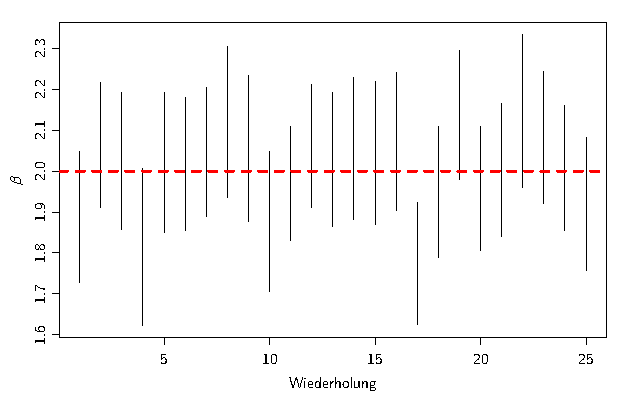
\includegraphics{Resources/Plots/CI_Illu2-1} \end{center}
\normalsize
\end{frame}

\begin{frame}{2.~\(\vtheta=\mR^\prime\vbeta\)}
\protect\hypertarget{vthetamrprimevbeta}{}
\begin{itemize}
\tightlist
\item
  Angenommen wir interessieren uns nun für eine \alert{Konfidenzregion}
  des Parametervektors \(\mR^\prime\vbeta\).

  \begin{itemize}
  \tightlist
  \item
    Z.B.~\(\vbeta\) selber, wenn \(\mR\) der Einheitsmatrix entspricht,
    oder auch einem Untervektor \(\vbeta_1\) von
    \(\vbeta=(\vbeta_1^\prime, \vbeta_2^\prime)^\prime\).
  \end{itemize}
\item
  \eqref{eq:Def C} sagt uns nun, dass \begin{eqnarray}
  \widehat{C} &=& \big\{\vr\mid \mathbb{H}_0\colon \mR^\prime\vbeta=\vr\ \text{kann z.N.}\ \alpha\ \text{nicht abgelehnt werden}\big\}\notag\\
  &\overset{\eqref{eq:t Test}}{=} & \big\{\vr\mid W\leq\chi_q^{2,-1}(1-\alpha)\big\}\label{eq:h8}\\
  &=& \Big\{\vr\mid n (\mR^\prime\widehat{\vbeta}- \vr)^\prime (\mR^\prime\widehat{\mV}_{\vbeta}^{\text{HC0}}\mR)^{-1}(\mR^\prime\widehat{\vbeta}- \vr)\leq\chi_q^{2,-1}(1-\alpha)\Big\}.\notag
  \end{eqnarray}
\end{itemize}
\end{frame}

\begin{frame}{2.~\(\vtheta=\mR^\prime\vbeta\)}
\protect\hypertarget{vthetamrprimevbeta-1}{}
\thmn

Unter den Annahmen von Theorem \ref{thm:Wald Test} ist \[
  \boxed{\ \widehat{C} = \Big\{\vr\mid n (\mR^\prime\widehat{\vbeta}- \vr)^\prime (\mR^\prime\widehat{\mV}_{\vbeta}^{\text{HC0}}\mR)^{-1}(\mR^\prime\widehat{\vbeta}- \vr)\leq\chi_q^{2,-1}(1-\alpha)\Big\}\ }
\] ein asymptotisches \((1-\alpha)\)-Konfidenzintervall für den
Parameter \(\mR^\prime\vbeta\).\medskip \endthmn

\begin{proof}
Folgt direkt aus \eqref{eq:h8} und Theorem \ref{thm:Wald Test}.
\end{proof}

\begin{itemize}
\tightlist
\item
  Es ist unmittelbar klar, dass \(\widehat{C}\) die Form einer
  \alert{Ellipse} hat.
\end{itemize}
\end{frame}

\hypertarget{instrumentvariablen}{%
\section{Instrumentvariablen}\label{instrumentvariablen}}

\begin{frame}{}
\protect\hypertarget{section-7}{}
\centerline{\textbf{Instrumentvariablen}}
\centerline{(Hansen, 2022, Kapitel 12)}
\end{frame}

\begin{frame}{Ausblick}
\protect\hypertarget{ausblick-2}{}
\begin{itemize}
\tightlist
\item
  In diesem Kapitel betrachten wir Modelle der Form
  \begin{equation}\label{eq:struc eq}
  \boxed{\ Y=X^\prime\vbeta+e,\qquad \E[Xe]\neq\vzero,\ }
  \end{equation} und sagen \(X\) ist \hil{endogen} für \(\vbeta\), wenn
  \(\E[Xe]\neq\vzero\).
\item
  D.h.~wir betrachten insbesondere

  \begin{itemize}
  \tightlist
  \item
    kein \alert{lineares Projektionsmodell} \[
    Y=X^\prime\vbeta^\ast+e^\ast,\qquad\vbeta^\ast=\E[XX^\prime]^{-1}\E[XY],\qquad\E[Xe^\ast]=\vzero.
    \]
  \item
    und kein \alert{lineares bedingter Erwartungswertmodell} \[
    Y=X^\prime\vbeta^{\ddagger}+\eps,\qquad \E[\eps\mid X]=\vzero,
    \] da dort ja gilt
    \(\E[X\eps]\overset{\eqref{eq:uncorr}}{=}\vzero\).
  \end{itemize}
\item
  Also wollen wir \eqref{eq:struc eq} als \alert{wahren DGP} betrachten
  -- allerdings einen, der Tücken mit sich bringt, wie wir auf der
  nächsten Folie sehen.
\item
  Um diese Tücken schon in der Benennung deutlich werden zu lassen,
  nennen wir \eqref{eq:struc eq} ein \hil{strukturelles Modell} und
  \(\vbeta\) einen \hil{strukturellen Parameter}.
\end{itemize}
\end{frame}

\begin{frame}{Ausblick}
\protect\hypertarget{ausblick-3}{}
\begin{itemize}
\tightlist
\item
  Was ist das \alert{Problem} des strukturellen Modells in
  \eqref{eq:struc eq}?
\item
  Wir können \alert{nur} aufgrund der Beobachtungen
  \((Y_i, X_i^\prime)\) nichts über den strukturellen Parameter
  \(\vbeta\) lernen, denn\ldots{}
\item
  \ldots{} KQ schätzt den \alert{linearen Projektionskoeffizienten}
  (Theorem \ref{thm:KQ cons}) anstatt den
  \alert{strukturellen Parameter} von Interesse: \begin{align}
  \widehat{\vbeta}\overset{\Pr}{\longrightarrow}\vbeta^\ast&=\E[XX^\prime]^{-1}\E[XY]\notag\\
  &=\E[XX^\prime]^{-1}\E[X(X^\prime\vbeta+e)]\notag\\
  &=\vbeta+\E[XX^\prime]^{-1}\E[Xe]\label{eq:bias beta}\\
  &\neq\vbeta.\notag
  \end{align}
\item
  Wir brauchen also \alert{mehr Informationen} als nur die
  \((Y_i, X_i^\prime)\), um etwas über \(\vbeta\) zu lernen -- das
  werden die \hil{Instrumente} sein\ldots{}
\item
  Aber zuerst wollen wir uns 3 Beispiele anschauen, wie strukturelle
  Modelle der Form \eqref{eq:struc eq} \alert{entstehen} können.
\end{itemize}
\end{frame}

\begin{frame}{Überblick}
\protect\hypertarget{uxfcberblick-23}{}
\begin{itemize}
\tightlist
\item
  \textbf{Beispiele}
\item
  Instrumente
\item
  IV Schätzer
\item
  TSLS Schätzer
\item
  Asymptotische Eigenschaften
\item
  Testen überidentifizierender Restriktionen
\item
  Endogenitätstest
\end{itemize}
\end{frame}

\begin{frame}{1. Regressionen mit ausgelassenen Variablen}
\protect\hypertarget{regressionen-mit-ausgelassenen-variablen}{}
\begin{itemize}
\tightlist
\item
  Nehmen wir an \(k=3\) und
  \(Y=\beta_0^\dagger +\beta_1^\dagger X_1 + \beta_2^\dagger X_2+u\) sei
  der \alert{wahre DGP}.
\item
  Aber wir können \(X_2\) \alert{nicht beobachten} und schreiben das
  Modell um zu \begin{equation}\label{eq:ovb mod}
  Y=\underbrace{\beta_0^\dagger + \beta_2^\dagger\E[X_2]}_{=\beta_0} +\underbrace{\beta_1^\dagger}_{=\beta_1} X_1 + \underbrace{\beta_2^\dagger (X_2 - \E[X_2]) + u.}_{=e}
  \end{equation}
\item
  Wenn \(X_1\) und \(X_2\) korrelieren, haben wir
  \(\E[X_1 e]\neq\vzero\) in \eqref{eq:ovb mod}.\medskip
\end{itemize}

\xmpl[Lohnregression]

\begin{itemize}
\tightlist
\item
  Unterstellen wir
  \(\log(wage)=\beta_0^\dagger+\beta_1^\dagger\cdot educ + \beta_2^\dagger\cdot ability+u\)
  als \alert{wahren DGP}.
\item
  Wegen der \alert{Unbeobachtbarkeit} von \emph{ability}, schätzen wir
  aber nur \[
  \log(wage)=\beta_0+\beta_1\cdot educ + e,\qquad e=\beta_2^\dagger\cdot (ability-\E[ability]) + u.
  \]
\item
  Da \emph{ability} und \emph{educ} (positiv) korrelieren, ist
  \(\E[educ\cdot e]\neq0\) die Folge.
\end{itemize}

\endxmpl
\end{frame}

\begin{frame}{2. Messfehler in den Regressoren}
\protect\hypertarget{messfehler-in-den-regressoren}{}
\begin{itemize}
\tightlist
\item
  Angenommen \(Y=(X^{\dagger})^\prime\vbeta+u\) mit
  \(\E[u\mid X^{\dagger}]=0\) sei der \alert{wahre DGP}.
\item
  Aber anstatt \(X^{\dagger}\) beobachten wir nur \(X=X^{\dagger}+\nu\),
  wobei \(\E[\nu]=\vzero\) und \(\nu\) unabhängig von \(X^{\dagger}\)
  und \(u\) ist; das ist der \hil{klassische Messfehler}!
\item
  Schreibe das Modell um, zu \[
  Y=(X^{\dagger})^\prime\vbeta+u=(X-\nu)^\prime\vbeta+u=X^\prime\vbeta + \underbrace{u-\nu^\prime\vbeta}_{=e}.
  \]
\item
  Wenn \(\vbeta\neq\vzero\) und \(\E[\nu\nu^\prime]>0\), dann ist \(X\)
  \alert{endogen}, denn \[
  \E[Xe] = \E\big[(X^{\dagger}+\nu)(u-\nu^\prime\vbeta)\big] = -\E[\nu\nu^\prime]\vbeta\neq\vzero.
  \]
\item
  Für \alert{$k=1$}, schätzt KQ dann wegen \eqref{eq:bias beta} den
  linearen Projektionskoeffizienten \[
  \beta^\ast=\beta + \frac{\E[Xe]}{\E[X^2]} = \beta\Big(1-\frac{\E[\nu^2]}{\E[X^2]}\Big).
  \]
\item
  Da \(\E[\nu^2]/\E[X^2]<1\), verzerrt dies die KQ Schätzung hin zur 0
  -- \hil{attenuation bias}!
\end{itemize}
\end{frame}

\begin{frame}{2. Messfehler in den Regressoren}
\protect\hypertarget{messfehler-in-den-regressoren-1}{}
\xmpl

\begin{itemize}
\tightlist
\item
  Betrachte die Paare \((Y,X)\), wobei \(X=X^\dagger+\nu\) mit
  \(\nu=\pm1\) mit Wkt.~\(1/2\).
\item
  Die 6 Kreise für die (messfehlerbehafteten) \((Y,X)\) strecken die
  Verteilung entlang der \(x\)-Achse aus, aber \alert{nicht} entlang der
  \(y\)-Achse.
\item
  Die Regressionslinie wird \alert{flacher} -- das ist der
  o.g.~attenuation bias.
\end{itemize}

\endxmpl
\end{frame}

\begin{frame}{2. Messfehler in den Regressoren}
\protect\hypertarget{messfehler-in-den-regressoren-2}{}
\footnotesize
\begin{center}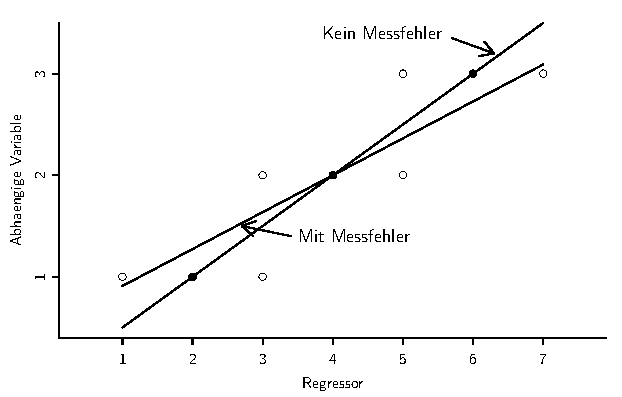
\includegraphics{Resources/Plots/Messfehler-1} \end{center}
\normalsize
\end{frame}

\begin{frame}{3. Simultane Gleichungssyteme}
\protect\hypertarget{simultane-gleichungssyteme}{}
\begin{itemize}
\tightlist
\item
  Betrachten Sie folgendes Beispiel zu \alert{Angebot und Nachfrage}.
\item
  Mit \(Q^d\) (\(Q^s\)) der nachgefragten (angebotenen) Menge und dem
  (nicht markträumenden) Preis \(\widetilde{P}\): \begin{align*}
  Q^d &= \beta_0^d+\beta_1^d \widetilde{P} + u^d,\\
  Q^s &= \beta_0^s+\beta_1^s \widetilde{P} + u^s,
  \end{align*} wobei \(\E[u^d]=\E[u^s]=\E[u^s u^d]=0\).
\item
  Was können wir über die \alert{Nachfrage- und Angebotskurve} lernen,
  wenn wir Preise \(P\) und Mengen \(Q\) nur im Gleichgewicht beobachten
  (also wenn \(Q^d=Q^s\))?
\item
  Im \alert{Gleichgewicht} gilt \[
  P=\frac{\beta_0^s-\beta_0^d+u^s-u^d}{\beta_1^d-\beta_1^s}.
  \]
\item
  Der Gleichgewichtspreis \(P\) ist \alert{endogen} in beiden
  Gleichungen, denn: \[
  \E[Pu^s] =\frac{\Var(u^s)}{\beta_1^d-\beta_1^s}\qquad\text{und}\qquad \E[Pu^d] =-\frac{\Var(u^d)}{\beta_1^d-\beta_1^s}.
  \]
\end{itemize}
\end{frame}

\begin{frame}{3. Simultane Gleichungssyteme}
\protect\hypertarget{simultane-gleichungssyteme-1}{}
\begin{itemize}
\tightlist
\item
  Aufgrund der Endogenität von \(P\) können wir also
  \alert{weder über die Nachfrage- noch über die Angebotskurve} etwas
  aus den beobachteten Gleichgewichtspreisen \((Q,P)\) lernen!
\item
  Z.B.~gibt es im Angebots- und Nachfragemodell
  \(Q^s=\widetilde{P}+u^s\) und \(Q^{d}=4-\widetilde{P}+u^d\) für
  Rademacher-verteilte \(u^{s}\) und \(u^d\) (d.h.~\(\pm1\) mit
  Wkt.~1/2) \alert{4 Gleichgewichtszustände}, also 4 Paare \((P,Q)\).
\end{itemize}

\footnotesize
\begin{center}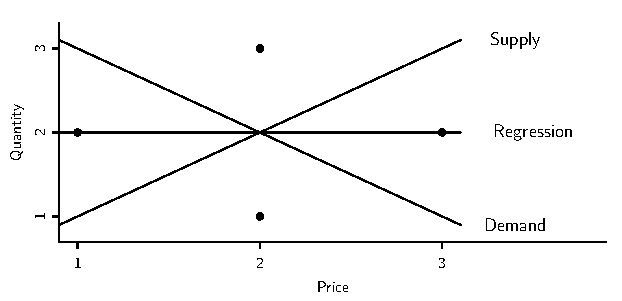
\includegraphics{Resources/Plots/DS-1} \end{center}
\normalsize
\end{frame}

\begin{frame}{Überblick}
\protect\hypertarget{uxfcberblick-24}{}
\begin{itemize}
\tightlist
\item
  Beispiele
\item
  \textbf{Instrumente}
\item
  IV Schätzer
\item
  TSLS Schätzer
\item
  Asymptotische Eigenschaften
\item
  Testen überidentifizierender Restriktionen
\item
  Endogenitätstest
\end{itemize}
\end{frame}

\begin{frame}{Das Problem}
\protect\hypertarget{das-problem}{}
\begin{itemize}
\tightlist
\item
  Wie oben gesagt, betrachten wir hier nun \alert{strukturelle Modelle:}
  \begin{equation}\label{eq:struc eq1}
  Y=X^\prime\vbeta+e,\qquad\E[Xe]\neq\vzero.
  \end{equation}
\item
  In vielen Anwendungen ist meist nur eine \alert{Teilmenge} \(X_2\) von
  \(k_2\) Regressoren in \(X\) endogen (d.h.~\(\E[X_2e]\neq\vzero\)).
\item
  Die restlichen \(k_1\) Regressoren \(X_1\), für die dann
  \(\E[X_1e]=\vzero\) gilt, nennen wir \hil{exogen}.
\item
  Wir können damit das strukturelle Modell auch schreiben als \[
  Y=X_1^\prime\vbeta_1+X_2^\prime\vbeta_2 + e,\qquad \E[Xe]\neq\vzero.
  \]
\item
  Um \(\vbeta=(\vbeta_1^\prime, \vbeta_2^\prime)^\prime\) konsistent zu
  schätzen, brauchen wir \alert{zusätzliche Informationen}.
\item
  Solche Informationen liefern uns \hil{Instrumente}\ldots{}
\end{itemize}
\end{frame}

\begin{frame}{Instrumente}
\protect\hypertarget{instrumente}{}
\defn\label{defn:IV} Der \((\ell\times1)\) Zufallsvektor \(Z\) ist eine
\hil{Instrumentvariable (IV)} für \eqref{eq:struc eq1}, falls
\begin{align}
  \E[Ze] &=\vzero & (\text{\hil{Instrumentexogenität}}),\label{eq:(12.5)}\\
  \E[Z Z^\prime] &>0 & (\text{\hil{Nicht-Redundanz}}),\label{eq:(12.6)}\\
  \rk\big(\E[ZX^\prime]\big)&=k & (\text{\hil{Instrumentrelevanz}}).\label{eq:(12.7)}
\end{align} \enddefn

\begin{itemize}
\tightlist
\item
  Im Folgenden diskutieren wir die einzelnen Teile der
  Definition\ldots{}
\end{itemize}
\end{frame}

\begin{frame}{Instrumentexogenität: \(\E[Ze]=\vzero\)}
\protect\hypertarget{instrumentexogenituxe4t-ezevzero}{}
\begin{itemize}
\tightlist
\item
  \eqref{eq:(12.5)}, also \(\E[Ze]=\vzero\), bezeichnen wir als die
  Bedingung der \hil{Instrumentexogenität}.
\item
  Als exogene Variablen erfüllen auch die \(X_1\) diese Annahme und
  sollten daher \alert{Teil von $Z$} sein.
\item
  Daher \alert{partitionieren} wir die Instrumente \(Z\) oft als \[
  Z=\begin{pmatrix}Z_1\\ Z_2\end{pmatrix}=\begin{pmatrix}X_1\\ Z_2\end{pmatrix}.
  \]
\item
  Die \(Z_1=X_1\) bezeichnen wir als die
  \hil{inkludierten exogenen Variablen} \ldots{}
\item
  \ldots{} und die \(Z_2\) als die
  \hil{exkludierten exogenen Variablen}.
\item
  Die \(Z_2\) sind also die Variablen,

  \begin{enumerate}
  \tightlist
  \item
    die potentiell im Modell für \(Y\) hätten auftauchen können (im
    Sinne, dass sie \alert{unkorreliert mit $e$} sind);
  \item
    aber einen \alert{wahren Koeffizienten von 0} in der strukturellen
    Gleichung \eqref{eq:struc eq1} haben (also keinen eigenständigen
    Einfluss auf \(Y\) haben).
  \end{enumerate}
\end{itemize}
\end{frame}

\begin{frame}{Nicht-Redundanz der Instrumente: \(\E[Z Z^\prime]>0\)}
\protect\hypertarget{nicht-redundanz-der-instrumente-ez-zprime0}{}
\begin{itemize}
\tightlist
\item
  Die Annahme \(\E[Z Z^\prime]>0\) schließt \alert{linear redundante}
  Instrumente aus.

  \begin{itemize}
  \tightlist
  \item
    Das ist ähnlich wie schon bei \(\E[X X^\prime]>0\) in Annahme
    \ref{ass:1}.
  \end{itemize}
\end{itemize}
\end{frame}

\begin{frame}{Instrumentrelevanz: \(\rk\big(\E[ZX^\prime]\big)=k\)}
\protect\hypertarget{instrumentrelevanz-rkbigezxprimebigk}{}
\begin{itemize}
\tightlist
\item
  Die Annahme
  \(\rk\big(\underset{(\ell\times k)}{\E[ZX^\prime]}\big)=k\) wird
  interpretiert als \hil{Instrumentrelevanz}.
\item
  Eine \alert{notwendige Bedingung} dafür ist \(\ell\geq k\), d.h.~wir
  brauchen mindestens so viele Instrumente wie Regressoren.
\item
  \alert{Woher} kommt die obige Interpretation als
  Instrumentrelevanz?\medskip
\end{itemize}

\lem\label{lem:help} Gelte \(\E[ZZ^\prime]>0\). Definiere \(\varPi\)
implizit durch \(\mathcal{P}(X\mid Z)=\varPi^\prime Z\), d.h.~nach
\eqref{eq:BLP eq} \(\varPi=\big(\E[ZZ^\prime]\big)^{-1}\E[ZX^\prime]\).
Dann gilt: \[
  \rk\big(\E[ZX^\prime]\big)=k \qquad\Longleftrightarrow\qquad \rk(\varPi)=k.
\] Ferner gilt: Im Fall \(\rk(\varPi)=k\) ist die Matrix
\(\varPi^\prime\E[ZX^\prime]\) invertierbar. \endlem
\end{frame}

\begin{frame}{Instrumentrelevanz: \(\rk\big(\E[ZX^\prime]\big)=k\)}
\protect\hypertarget{instrumentrelevanz-rkbigezxprimebigk-1}{}
\begin{block}{Beweis von Lemma \ref{lem:help}}
Schreibe das lineare Projektionsmodell als $X=\varPi^\prime Z + \nu$ mit $\E[Z\nu^\prime]=\vzero$. Daher
\begin{equation}\label{eq:impl Proj}
  \E[ZX^\prime]=\E[Z(\varPi^\prime Z + \nu)^\prime]=\E[ZZ^\prime]\varPi.
\end{equation}
Daraus:
\begin{eqnarray*}
  \rk\big(\E[ZX^\prime]\big) &\overset{\eqref{eq:impl Proj}}{=}&\rk\big(\E[ZZ^\prime]\varPi\big)\overset{\text{Prop.}}{\underset{\zref{S-rules1}.\zref{S-it:19.7}}{\leq}}\rk\big(\varPi\big),\\
  \rk\big(\varPi\big) &=& \rk\big(\E[ZZ^\prime]^{-1}\E[ZZ^\prime]\varPi\big)\overset{\text{Prop.}}{\underset{\zref{S-rules1}.\zref{S-it:19.7}}{\leq}} \rk\big(\E[ZZ^\prime]\varPi\big)\overset{\eqref{eq:impl Proj}}{=}\rk\big(\E[ZX^\prime]\big).
\end{eqnarray*}
Aus diesen beiden Ungleichungen folgt $\rk(\varPi)=\rk\big(\E[ZX^\prime]\big)$, also insbesondere die obige Äquivalenz.\bigskip

Wenn $\rk(\varPi)=k$ (also $\varPi$ hat vollen Rang), dann ist
\[
  \varPi^\prime\E[ZX^\prime]\overset{\eqref{eq:impl Proj}}{=}\varPi^\prime\E[ZZ^\prime]\varPi
\]
invertierbar, weil $\varPi$ vollen Rang hat und $\E[ZZ^\prime]>0$.
\end{block}
\end{frame}

\begin{frame}{Instrumentrelevanz: \(\rk\big(\E[ZX^\prime]\big)=k\)}
\protect\hypertarget{instrumentrelevanz-rkbigezxprimebigk-2}{}
\begin{itemize}
\tightlist
\item
  \alert{Interpretation:} Betrachte den Fall \(k=\ell\) und nur \(X_k\)
  ist endogen. Sei daher \(Z_j=X_j\) für alle \(j=1,\ldots,k-1\).
\item
  In diesem Fall folgt aus \(\mathcal{P}(X\mid Z)=\varPi^\prime Z\): \[
  \varPi^\prime=\begin{pmatrix}
    1 & 0 & \ldots & 0 & 0\\
    0 & 1 & \ldots & 0 & 0\\
    \vdots & \vdots & \ddots& \vdots & \vdots\\
    0 & 0 & \ldots & 1 & 0\\
    \pi_1 & \pi_2 & \ldots & \pi_{k-1} & \pi_k
  \end{pmatrix}.
  \]
\item
  Die Rangbedingung verlangt (wegen Lemma \ref{lem:help}) daher
  \alert{$\pi_k\neq0$}, d.h.~das Instrument \(Z_k\) muss
  \alert{mit $X_k$ korrelieren nachdem für $X_1,\ldots,X_{k-1}$ kontrolliert wurde.}
\item
  M.a.W.: Das Instrument muss \alert{relevant} für den endogenen
  Regressor sein -- daher der Name der Instrumentrelevanz!
\end{itemize}
\end{frame}

\begin{frame}{Zusammenfassung}
\protect\hypertarget{zusammenfassung-2}{}
\begin{itemize}
\tightlist
\item
  \alert{Instrumentexogenität} verlangt: Instrumente \(Z_2\) haben
  keinen eigenen Einfluss auf \(Y\).
\item
  \alert{Instrumentrelevanz} verlangt: Instrumente \(Z_2\) korrelieren
  mit den endogenen Variablen nachdem für die exogenen kontrolliert
  wurde.
\item
  \alert{Zusammengenommen:} Die exkludierten Instrumente \(Z_2\) sind
  kausal für die endogenen Variablen \(X_2\), aber beeinflussen \(Y\)
  nicht kausal, außer durch \(X_2\).
\end{itemize}

\xmpl

\begin{itemize}
\tightlist
\item
  \alert{Messfehler:} Wenn \(X\) eine Version von \(X^\dagger\) mit
  Messfehler ist, dann ist ein valides Instrument \(Z_2\) eine
  alternative Messung von \(X^\dagger\), deren Messfehler unabhängig von
  dem in \(X\) ist.
\item
  \alert{Angebot und Nachfrage:} Ein valides Instrument \(Z_2\) für
  \(P\) in der Nachfragegleichung ist eine Variable, die nicht direkt
  die Nachfrage beeinflusst, außer indirekt über das Angebot
  (typischerweise Variable mit Bezug zu Produktionskosten).
\item
  \alert{Ausgelassene Variablen:} Instrument beeinflusst Regressor
  (z.B.~\(educ\)), aber nicht direkt die abhängige Variable
  (z.B.~\(\log(wage)\)), außer durch indirekten Effekt über Regressor.
\end{itemize}

\endxmpl
\end{frame}

\begin{frame}{Überblick}
\protect\hypertarget{uxfcberblick-25}{}
\begin{itemize}
\tightlist
\item
  Beispiele
\item
  Instrumente
\item
  \textbf{IV Schätzer}
\item
  TSLS Schätzer
\item
  Asymptotische Eigenschaften
\item
  Testen überidentifizierender Restriktionen
\item
  Endogenitätstest
\end{itemize}
\end{frame}

\begin{frame}{IV Schätzer}
\protect\hypertarget{iv-schuxe4tzer}{}
\begin{itemize}
\tightlist
\item
  Wir betrachten hier erstmal den \hil{exakt identifizierten} Fall
  \alert{$\ell=k$}.
\item
  Wie können wir
  \alert{Instrumente nun benutzen, um $\vbeta$ konsistent} im
  strukturellen Modell \eqref{eq:struc eq1} zu schätzen?
\item
  Ganz einfach: \begin{equation}\label{eq:beta IV eq}
  \E[ZY]\overset{\eqref{eq:struc eq1}}{=}\E[Z(X^\prime\vbeta+e)]=\E[ZX^\prime]\vbeta + \underbrace{\E[Ze]}_{\overset{\eqref{eq:(12.5)}}{=}\vzero}=\E[ZX^\prime]\vbeta.
  \end{equation}
\item
  Im Fall \(\ell=k\) ist \(\E[ZX^\prime]\) eine symmetrische
  \(k\times k\)-Matrix mit \(\rk(\E[ZX^\prime])=k\) (wegen
  \eqref{eq:(12.7)}).
\item
  Proposition~\zref{S-rules3}.\zref{S-it:21.6} impliziert daher, dass
  \((\E[ZX^\prime])^{-1}\) existiert und somit \[
  \vbeta=\big(\E[ZX^\prime]\big)^{-1}\E[ZY].
  \]
\end{itemize}
\end{frame}

\begin{frame}{IV Schätzer}
\protect\hypertarget{iv-schuxe4tzer-1}{}
\begin{itemize}
\tightlist
\item
  Wir haben eine Formel für \(\vbeta\), aber für die Schätzung brauchen
  wir Daten.\medskip
\end{itemize}

\ass\label{ass:iid IV} Die Variablen
\((Y_1,X_1,Z_1),\ldots,(Y_n,X_n,Z_n)\) sind u.i.v. \endass

\begin{itemize}
\tightlist
\item
  Ähnlich wie oben ist ein natürlicher Schätzer von
  \(\vbeta=\big(\E[ZX^\prime]\big)^{-1}\E[ZY]\) dann der
  \hil{Instrumentvariablen-Schätzer} \begin{equation}\label{eq:IV}
  \boxed{\ \widehat{\vbeta}_{\text{IV}} = \bigg(\frac{1}{n}\sum_{i=1}^{n}Z_iX_i^\prime\bigg)^{-1}\bigg(\frac{1}{n}\sum_{i=1}^{n}Z_iY_i\bigg). \ }
  \end{equation}
\item
  Für \(Z=X\) ist der IV-Schätzer natürlich wieder der KQ Schätzer,
  d.h.~\(\widehat{\vbeta}_{\text{IV}}=\widehat{\vbeta}\).
\end{itemize}
\end{frame}

\begin{frame}{IV Schätzer}
\protect\hypertarget{iv-schuxe4tzer-2}{}
\xmpl

\begin{itemize}
\tightlist
\item
  Betrachte eine Regression \(Y=\beta_1+\beta_2 X_2+e\) mit
  \alert{endogenem} \(X_2\in\mathbb{R}\).
\item
  In diesem Fall ist der \alert{IV-Schätzer} mit Instrument \(Z_2\)
  (nach durchmultiplizieren mit
  \(\frac{1}{n}\sum_{i=1}^{n}(Z_{2,i} - \overline{Z}_{2,n})^2\) in
  Zähler und Nenner) \begin{align*}
  \widehat{\vbeta}_{\text{IV}} &= \frac{\frac{1}{n}\sum_{i=1}^{n}(Z_{2,i} - \overline{Z}_{2,n})Y_i\ /\ \frac{1}{n}\sum_{i=1}^{n}(Z_{2,i} - \overline{Z}_{2,n})^2}{\frac{1}{n}\sum_{i=1}^{n}(Z_{2,i} - \overline{Z}_{2,n})X_{2,i}\ /\ \frac{1}{n}\sum_{i=1}^{n}(Z_{2,i} - \overline{Z}_{2,n})^2}\\
  &= \frac{\text{Steigungskoeffizient einer Regression von }Y\text{ auf }Z_2}{\text{Steigungskoeffizient einer Regression von }X_2\text{ auf }Z_2}.
  \end{align*}
\item
  Das macht \alert{Sinn}, weil \begin{align}
  X_2 &= \pi_1+\pi_2 Z_2 + v,\label{eq:fs ex}\\
  Y &=\beta_1 + \beta_2X_2 + e \overset{\eqref{eq:fs ex}}{=} \underbrace{\beta_1+\beta_2\pi_1}_{=\beta_1^\ast} + \underbrace{\beta_2\pi_2}_{\beta_2^\ast} Z_2 + \underbrace{e+\beta_2v.}_{=e^\ast}\notag
  \end{align}
\end{itemize}

\endxmpl
\end{frame}

\begin{frame}{Mehr zum IV Schätzer}
\protect\hypertarget{mehr-zum-iv-schuxe4tzer}{}
\begin{itemize}
\tightlist
\item
  Wegen
  \(\widehat{\vbeta}_{\text{IV}} = \big(\frac{1}{n}\sum_{i=1}^{n}Z_iX_i^\prime\big)^{-1}\big(\frac{1}{n}\sum_{i=1}^{n}Z_iY_i\big)\)
  folgt unmittelbar \[
  \frac{1}{n}\sum_{i=1}^{n}Z_i\big(Y_i-X_i^\prime\widehat{\vbeta}_{\text{IV}}\big)=\vzero.
  \]
\item
  D.h.~die \hil{Residuen}
  \(\widehat{e}_i=Y_i-X_i^\prime\widehat{\vbeta}_{\text{IV}}\) sind
  \alert{orthogonal zu den Instrumenten} \(Z_i\): \[
  \frac{1}{n}\sum_{i=1}^{n}Z_i\widehat{e}_i=\vzero.
  \]
\item
  Setzen wir \(\mZ=(Z_1,\ldots,Z_n)^\prime\), so schreibt sich der
  IV-Schätzer in \alert{Matrixnotation} als \[
  \widehat{\vbeta}_{\text{IV}}=(\mZ^\prime\mX)^{-1}\mZ^\prime\mY.
  \]
\end{itemize}
\end{frame}

\begin{frame}{Beispiel}
\protect\hypertarget{beispiel-3}{}
\xmpl[Card (1995)]\label{ex:Card5}

\begin{itemize}
\tightlist
\item
  Betrachte die KQ Regression in \eqref{eq:Card1}, d.h.
  \begin{multline*}
  \log(wage) =  \beta_0+ \beta_1\cdot educ + \beta_2\cdot exper + \beta_3\cdot(exper/100)^2 + \\
   \beta_4\cdot black + \beta_5\cdot south + \beta_6\cdot urban + e.
  \end{multline*}
\item
  \(e\) enthält die ausgelassene Variable \(ability\), die \(educ\)
  beeinflussen könnte.
\item
  Ein Instrument könnte der Dummy \[
  Z=\text{"In einem Bezirk mit 4-Jahres College aufgewachsen"}
  \] sein (\alert{nearc4}), denn:

  \begin{enumerate}
  \tightlist
  \item
    \alert{Instrumentexogenität:} Tatsache, ob jemand nahe eines College
    aufgewachsen ist, sollte nichts mit \(ability\) zu tun haben.
  \item
    \alert{Instrumentrelevanz:} Nah am College zu wohnen, reduziert
    Wohnungskosten, so dass College eher besucht wird (\(nearc4\) und
    \(educ\) korrelieren positiv).
  \end{enumerate}
\end{itemize}

\endxmpl
\end{frame}

\begin{frame}[fragile]{\R Beispiel}
\protect\hypertarget{beispiel-4}{}
\footnotesize

\begin{Shaded}
\begin{Highlighting}[]
\CommentTok{\# IV estimation}
\NormalTok{IV }\OtherTok{\textless{}{-}} \FunctionTok{ivreg}\NormalTok{(lwage76 }\SpecialCharTok{\textasciitilde{}}\NormalTok{ ed76 }\SpecialCharTok{+}\NormalTok{ exper }\SpecialCharTok{+} \FunctionTok{I}\NormalTok{(exper}\SpecialCharTok{\^{}}\DecValTok{2}\SpecialCharTok{/}\DecValTok{100}\NormalTok{) }\SpecialCharTok{+}\NormalTok{ black }\SpecialCharTok{+}\NormalTok{ reg76r }\SpecialCharTok{+}\NormalTok{ smsa76r}
                  \SpecialCharTok{|}\NormalTok{ nearc4 }\SpecialCharTok{+}\NormalTok{ exper }\SpecialCharTok{+} \FunctionTok{I}\NormalTok{(exper}\SpecialCharTok{\^{}}\DecValTok{2}\SpecialCharTok{/}\DecValTok{100}\NormalTok{) }\SpecialCharTok{+}\NormalTok{ black }\SpecialCharTok{+}\NormalTok{ reg76r }\SpecialCharTok{+}\NormalTok{ smsa76r, }\AttributeTok{data=}\NormalTok{card)}
\NormalTok{IV}
\end{Highlighting}
\end{Shaded}

\begin{verbatim}
## 
## Call:
## ivreg(formula = lwage76 ~ ed76 + exper + I(exper^2/100) + black +     reg76r + smsa76r | nearc4 + exper + I(exper^2/100) + black +     reg76r + smsa76r, data = card)
## 
## Coefficients:
##    (Intercept)            ed76           exper  I(exper^2/100)           black  
##          3.753           0.132           0.107          -0.228          -0.131  
##         reg76r         smsa76r  
##         -0.105           0.131
\end{verbatim}

\normalsize

\xmpl[*]

\begin{itemize}
\tightlist
\item
  \alert{Erstaunlich:} Der Koeffizient von \(educ\) ist im Vergleich zur
  KQ Schätzung in Beispiel~\ref{ex:Card1} von 0.074 auf 0.132 gestiegen
  -- ein zusätzliches Jahr in Ausbildung erhöht das durchschnittliche
  Gehalt nun um 13.2\%!
\item
  Wir hätten erwartet, dass KQ den (wahrscheinlich) positiven Effekt von
  \(ability\) der Variable \(educ\) zuschlägt und somit den
  \alert{wahren Einfluss von $educ$ auf $log(wage)$ überschätzt}.
\end{itemize}

\endxmpl
\end{frame}

\begin{frame}{Überblick}
\protect\hypertarget{uxfcberblick-26}{}
\begin{itemize}
\tightlist
\item
  Beispiele
\item
  Instrumente
\item
  IV Schätzer
\item
  \textbf{TSLS Schätzer}
\item
  Asymptotische Eigenschaften
\item
  Testen überidentifizierender Restriktionen
\item
  Endogenitätstest
\end{itemize}
\end{frame}

\begin{frame}{TSLS Schätzer}
\protect\hypertarget{tsls-schuxe4tzer}{}
\begin{itemize}
\tightlist
\item
  Wir betrachten nun den \hil{überidentifizierten} Fall
  \alert{$\ell>k$}, d.h.~mehr exkludierte Intrumente als endogene
  Variablen!
\item
  Wir können die \((\ell\times k)\)-Matrix \(\E[ZX^\prime]\) nicht mehr
  invertieren, weil sie noch nicht einmal mehr symmetrisch ist -- wir
  brauchen eine \alert{andere Idee}\ldots{}
\item
  Multipliziere \eqref{eq:beta IV eq} durch mit \(\varPi^\prime\): \[
  \varPi^\prime\E[ZY] = \varPi^\prime\E[ZX^\prime]\vbeta.
  \]
\item
  Unter unserer Bedingung \(\rk(\E[ZX^\prime])=k\) (siehe
  \eqref{eq:(12.7)}) ist aber nach Lemma \ref{lem:help} die Matrix
  \(\varPi^\prime\E[ZX^\prime]\) invertierbar, so dass \[
  \vbeta = \big(\varPi^\prime\E[ZX^\prime]\big)^{-1} \varPi^\prime\E[ZY].
  \]
\item
  Schätzer für \(\E[ZX^\prime]\) und \(\E[ZY]\) haben wir vorhin schon
  gesehen, aber \alert{wie schätzen wir $\varPi$}?
\end{itemize}
\end{frame}

\begin{frame}{TSLS Schätzer}
\protect\hypertarget{tsls-schuxe4tzer-1}{}
\begin{itemize}
\tightlist
\item
  \eqref{eq:(12.7)} erlaubt uns \eqref{eq:impl Proj} zu schreiben als \[
  \varPi=\big(\E[ZZ^\prime]\big)^{-1}\E[ZX^\prime].
  \]
\item
  Ein natürlicher \alert{Schätzer} von \(\varPi\) ist also
  \begin{equation}\label{eq:Proj Pi}
  \widehat{\varPi}=\bigg(\frac{1}{n}\sum_{i=1}^{n}Z_iZ_i^\prime\bigg)^{-1}\frac{1}{n}\sum_{i=1}^{n}Z_iX_i^\prime.
  \end{equation}
\item
  Ein natürlicher Schätzer von
  \(\vbeta = \big(\varPi^\prime\E[ZX^\prime]\big)^{-1} \varPi^\prime\E[ZY]\)
  ist daher der \hil{Two-Stage Least Squares (TSLS) Schätzer}
  \begin{equation}\label{eq:TSLS}
  \boxed{ \widehat{\vbeta}_{\text{TSLS}}= \Bigg(\widehat{\varPi}^\prime\bigg(\frac{1}{n}\sum_{i=1}^{n}Z_iX_i^\prime\bigg)\Bigg)^{-1}\widehat{\varPi}^\prime\bigg(\frac{1}{n}\sum_{i=1}^{n}Z_iY_i\bigg). }
  \end{equation}
\end{itemize}
\end{frame}

\begin{frame}{Zwei Interpretationen}
\protect\hypertarget{zwei-interpretationen}{}
\begin{itemize}
\tightlist
\item
  \alert{Zwei Interpretationen} von
  \(\widehat{\vbeta}_{\text{TSLS}}= \Big(\widehat{\varPi}^\prime\big(\frac{1}{n}\sum_{i=1}^{n}Z_iX_i^\prime\big)\Big)^{-1}\widehat{\varPi}\big(\frac{1}{n}\sum_{i=1}^{n}Z_iY_i\big)\):
  \begin{align}
  X_i & \overset{\text{siehe}}{\underset{\eqref{eq:Zerl fit resid}}{=}}\widehat{\varPi}^\prime Z_i + \widehat{V}_i,&& \widehat{\varPi}=\bigg(\frac{1}{n}\sum_{i=1}^{n}Z_iZ_i^\prime\bigg)^{-1}\frac{1}{n}\sum_{i=1}^{n}Z_iX_i^\prime,\notag\\
  \widehat{X}_i & \overset{\text{Def.}}{\underset{\ref{defn:Aw and Resids}}{=}}\widehat{\varPi}^\prime Z_i, &&\frac{1}{n}\sum_{i=1}^{n}Z_iX_i^\prime = \frac{1}{n}\sum_{i=1}^{n}Z_iZ_i^\prime\widehat{\varPi}.\label{eq:h11}
  \end{align}
\end{itemize}

\begin{enumerate}
\item
  TSLS ist
  \alert{IV mit $k$ linear kombinierten Instrumenten $\widehat{X}_i = \widehat{\varPi}^\prime Z_i$}
  (vgl.~\eqref{eq:IV}): \begin{equation*}
    \widehat{\vbeta}_{\text{TSLS}} =\bigg(\frac{1}{n}\sum_{i=1}^{n}\underbrace{\widehat{\varPi}^\prime Z_i}_{=\widehat{X}_i}X_i^\prime\bigg)^{-1}\bigg(\frac{1}{n}\sum_{i=1}^{n}\underbrace{\widehat{\varPi}^{\prime}Z_i}_{=\widehat{X}_i}Y_i\bigg).
  \end{equation*}
\item
  TSLS ist \alert{KQ mit Regressoren $\widehat{X}_i$}
  (vgl.~\eqref{eq:beta hat ausf}): \begin{equation}\label{eq:TSLS why}
    \widehat{\vbeta}_{\text{TSLS}} \overset{\eqref{eq:h11}}{=}\bigg(\frac{1}{n}\sum_{i=1}^{n}\underbrace{\widehat{\varPi}^\prime Z_i}_{=\widehat{X}_i}\underbrace{Z_i^\prime \widehat{\varPi}}_{=\widehat{X}_i^\prime}\bigg)^{-1}\bigg(\frac{1}{n}\sum_{i=1}^{n}\underbrace{\widehat{\varPi}^{\prime}Z_i}_{=\widehat{X}_i}Y_i\bigg).
  \end{equation}
\end{enumerate}
\end{frame}

\begin{frame}{Zwei Interpretationen}
\protect\hypertarget{zwei-interpretationen-1}{}
\begin{itemize}
\tightlist
\item
  Die zweite Interpretation \eqref{eq:TSLS why} liefert den
  \alert{Grund für den Namen:}
\end{itemize}

\begin{block}{Alternative Berechnung des TSLS Schätzers}
\begin{enumerate}
  \item Regressiere (jede Komponente von) $X_i$ auf $Z_i$ um $\widehat{X}_i=\widehat{\varPi}^\prime Z_i$ zu erhalten.
    \begin{itemize}
      \item Das Modell $X_i=\varPi^\prime Z_i + V_i$ wird \hil{reduzierte Form} genannt.
    \end{itemize}
  \item Regressiere $Y_i$ auf $\widehat{X}_i$ um $\widehat{\vbeta}_{\text{TSLS}}$ zu erhalten. 
\end{enumerate}\medskip
\alert{Obacht:} Die einfachen KQ Standardfehler aus dem 2.\ Schritt sind falsch -- wie man es richtig macht, sehen wir gleich.
\end{block}
\end{frame}

\begin{frame}{Mehr zum TSLS Schätzer}
\protect\hypertarget{mehr-zum-tsls-schuxe4tzer}{}
\begin{itemize}
\tightlist
\item
  Aus der Definition von \(\widehat{\vbeta}_{\text{TSLS}}\) folgt \[
  \vzero=\frac{1}{n}\sum_{i=1}^{n} \widehat{\varPi} Z_i\big(Y_i-X_i^\prime\widehat{\vbeta}_{\text{TSLS}}\big)=\frac{1}{n}\sum_{i=1}^{n} \widehat{\varPi} Z_i\widehat{e}_i.
  \]
\item
  D.h.~die Residuen
  \(\widehat{e}_i=Y_i-X_i^\prime\widehat{\vbeta}_{\text{TSLS}}\) sind
  \alert{orthogonal} zu allen exogenen Regressoren, aber
  \alert{nicht unbedingt orthogonal} zu den anderen Regressoren.
\item
  IV ist ein \alert{Spezialfall} von TSLS, denn im exakt identifizierten
  Fall \(\ell=k\) gilt: \begin{align*}
  \widehat{\vbeta}_{\text{TSLS}} &\overset{\eqref{eq:Proj Pi}}{\underset{\eqref{eq:TSLS}}{=}} \Bigg(\bigg(\frac{1}{n}\sum_{i=1}^{n}Z_iX_i^\prime\bigg)^\prime \bigg(\frac{1}{n}\sum_{i=1}^{n}Z_iZ_i^\prime\bigg)^{-1}\bigg(\frac{1}{n}\sum_{i=1}^{n}Z_iX_i^\prime\bigg)\Bigg)^{-1}\times\\
  &\hspace{2cm}\bigg(\frac{1}{n}\sum_{i=1}^{n}Z_iX_i^\prime\bigg)^\prime \bigg(\frac{1}{n}\sum_{i=1}^{n}Z_iZ_i^\prime\bigg)^{-1}\bigg(\frac{1}{n}\sum_{i=1}^{n}Z_iY_i\bigg)\\
  &= \bigg(\frac{1}{n}\sum_{i=1}^{n}Z_iX_i^\prime\bigg)^{-1}\bigg(\frac{1}{n}\sum_{i=1}^{n}Z_iY_i\bigg)=\widehat{\vbeta}_{\text{IV}}.
  \end{align*}
\end{itemize}
\end{frame}

\begin{frame}[fragile,allowframebreaks]{\R Beispiel}
\protect\hypertarget{beispiel-5}{}
\xmpl[*]

\begin{itemize}
\tightlist
\item
  Händisches Ausrechnen des IV Schätzers nach 2-Schritt Verfahren
  liefert \alert{identische Werte.}
\end{itemize}

\endxmpl

\footnotesize

\begin{Shaded}
\begin{Highlighting}[]
\CommentTok{\# Standard KQ}
\NormalTok{KQ   }\OtherTok{\textless{}{-}} \FunctionTok{lm}\NormalTok{(lwage76 }\SpecialCharTok{\textasciitilde{}}\NormalTok{ ed76 }\SpecialCharTok{+}\NormalTok{ exper }\SpecialCharTok{+} \FunctionTok{I}\NormalTok{(exper}\SpecialCharTok{\^{}}\DecValTok{2}\SpecialCharTok{/}\DecValTok{100}\NormalTok{) }\SpecialCharTok{+}\NormalTok{ black }\SpecialCharTok{+} 
\NormalTok{                        reg76r }\SpecialCharTok{+}\NormalTok{ smsa76r, }\AttributeTok{data=}\NormalTok{card)}

\CommentTok{\# Standard IV}
\NormalTok{IV   }\OtherTok{\textless{}{-}} \FunctionTok{ivreg}\NormalTok{(lwage76 }\SpecialCharTok{\textasciitilde{}}\NormalTok{ ed76 }\SpecialCharTok{+}\NormalTok{ exper }\SpecialCharTok{+} \FunctionTok{I}\NormalTok{(exper}\SpecialCharTok{\^{}}\DecValTok{2}\SpecialCharTok{/}\DecValTok{100}\NormalTok{) }\SpecialCharTok{+}\NormalTok{ black }\SpecialCharTok{+}\NormalTok{ reg76r }\SpecialCharTok{+}\NormalTok{ smsa76r}
                  \SpecialCharTok{|}\NormalTok{ nearc4 }\SpecialCharTok{+}\NormalTok{ exper }\SpecialCharTok{+} \FunctionTok{I}\NormalTok{(exper}\SpecialCharTok{\^{}}\DecValTok{2}\SpecialCharTok{/}\DecValTok{100}\NormalTok{) }\SpecialCharTok{+}\NormalTok{ black }\SpecialCharTok{+}\NormalTok{ reg76r }\SpecialCharTok{+}\NormalTok{ smsa76r, }\AttributeTok{data=}\NormalTok{card)}

\CommentTok{\# Reduzierte Form}
\NormalTok{redf }\OtherTok{\textless{}{-}} \FunctionTok{lm}\NormalTok{(ed76 }\SpecialCharTok{\textasciitilde{}}\NormalTok{ nearc4 }\SpecialCharTok{+}\NormalTok{ exper }\SpecialCharTok{+} \FunctionTok{I}\NormalTok{(exper}\SpecialCharTok{\^{}}\DecValTok{2}\SpecialCharTok{/}\DecValTok{100}\NormalTok{) }\SpecialCharTok{+}\NormalTok{ black }\SpecialCharTok{+}\NormalTok{ reg76r }\SpecialCharTok{+}\NormalTok{ smsa76r, }\AttributeTok{data=}\NormalTok{card)}

\CommentTok{\# TSLS by hand with incorrect standard errors (although by very little here)}
\NormalTok{ivbyhand }\OtherTok{\textless{}{-}} \FunctionTok{lm}\NormalTok{(lwage76 }\SpecialCharTok{\textasciitilde{}} \FunctionTok{fitted}\NormalTok{(redf) }\SpecialCharTok{+}\NormalTok{ exper }\SpecialCharTok{+} \FunctionTok{I}\NormalTok{(exper}\SpecialCharTok{\^{}}\DecValTok{2}\SpecialCharTok{/}\DecValTok{100}\NormalTok{) }\SpecialCharTok{+}\NormalTok{ black }\SpecialCharTok{+}\NormalTok{ reg76r }\SpecialCharTok{+}\NormalTok{ smsa76r, }
                                                                                \AttributeTok{data=}\NormalTok{card)}
\CommentTok{\# Pretty regression table of selected coefficients}
\FunctionTok{stargazer}\NormalTok{(KQ, IV, redf, ivbyhand, }\AttributeTok{type=}\StringTok{"text"}\NormalTok{,}
\AttributeTok{keep=}\FunctionTok{c}\NormalTok{(}\StringTok{"ed"}\NormalTok{, }\StringTok{"near"}\NormalTok{, }\StringTok{"exp"}\NormalTok{, }\StringTok{"bl"}\NormalTok{), }\AttributeTok{keep.stat=}\FunctionTok{c}\NormalTok{(}\StringTok{"n"}\NormalTok{, }\StringTok{"rsq"}\NormalTok{))}
\end{Highlighting}
\end{Shaded}

\begin{verbatim}
## 
## ========================================================
##                          Dependent variable:            
##               ------------------------------------------
##                      lwage76           ed76     lwage76 
##                  OLS    instrumental    OLS       OLS   
##                           variable                      
##                  (1)        (2)         (3)       (4)   
## --------------------------------------------------------
## ed76          0.074***    0.132***                      
##                (0.004)    (0.049)                       
##                                                         
## nearc4                               0.337***           
##                                       (0.083)           
##                                                         
## fitted(redf)                                   0.132*** 
##                                                 (0.050) 
##                                                         
## exper         0.084***    0.107***   -0.410*** 0.107*** 
##                (0.007)    (0.021)     (0.034)   (0.022) 
##                                                         
## I(exper2/100) -0.224***  -0.228***     0.073   -0.228***
##                (0.032)    (0.033)     (0.165)   (0.034) 
##                                                         
## black         -0.190***   -0.131**   -1.006*** -0.131** 
##                (0.018)    (0.053)     (0.090)   (0.054) 
##                                                         
## --------------------------------------------------------
## Observations    3,010      3,010       3,010     3,010  
## R2              0.291      0.225       0.474     0.187  
## ========================================================
## Note:                        *p<0.1; **p<0.05; ***p<0.01
\end{verbatim}

\normalsize
\end{frame}

\begin{frame}{Überblick}
\protect\hypertarget{uxfcberblick-27}{}
\begin{itemize}
\tightlist
\item
  Beispiele
\item
  Instrumente
\item
  IV Schätzer
\item
  TSLS Schätzer
\item
  \textbf{Asymptotische Eigenschaften}
\item
  Testen überidentifizierender Restriktionen
\item
  Endogenitätstest
\end{itemize}
\end{frame}

\begin{frame}{Asymptotische Eigenschaften}
\protect\hypertarget{asymptotische-eigenschaften}{}
\begin{itemize}
\tightlist
\item
  Wir beschäftigen uns jetzt mit den asymptotischen Eigenschaften des
  TSLS Schätzers.

  \begin{itemize}
  \tightlist
  \item
    \alert{Konsistenz} und \alert{asymptotische Normalität.}
  \end{itemize}
\item
  Dazu schreiben wir den TSLS Schätzer aus \eqref{eq:TSLS} in
  \alert{Matrixnotation:} \begin{align}
  \widehat{\vbeta}_{\text{TSLS}} & = \big(\mX^\prime\mZ (\mZ^\prime\mZ)^{-1} \mX^\prime\mZ\big)^{-1}\mZ^\prime\mX(\mZ^\prime\mZ)^{-1}\mZ^\prime\mY\notag\\
  &= \big(\mX^\prime\mZ (\mZ^\prime\mZ)^{-1} \mZ^\prime\mX\big)^{-1}\mX^\prime\mZ(\mZ^\prime\mZ)^{-1}\mZ^\prime(\mX\vbeta+\ve)\notag\\
  &= \vbeta + \big(\mX^\prime\mZ (\mZ^\prime\mZ)^{-1} \mZ^\prime\mX\big)^{-1}\mX^\prime\mZ(\mZ^\prime\mZ)^{-1}\mZ^\prime\ve.\label{eq:TSLS help}
  \end{align}
\end{itemize}
\end{frame}

\begin{frame}{Konsistenz}
\protect\hypertarget{konsistenz-1}{}
\thmn[Hansen (2022, Theorem 12.1)]\label{thm:cons TSLS} Seien \(Z\)
Instrumentvariablen für \(X\) (d.h.~Definition \ref{defn:IV} gilt für
\(Z\)). Gelten Annahme \ref{ass:iid IV} und \[
  \E[Y^2]<\infty,\quad\E\Vert X\Vert^2<\infty,\quad\E\Vert Z\Vert^2<\infty.
\] Dann gilt: \[
  \boxed{\ \widehat{\vbeta}_{\text{TSLS}} \overset{\Pr}{\longrightarrow}\vbeta.\ }
\] \endthmn

\begin{itemize}
\tightlist
\item
  Ein \alert{tolles Resultat:} Instrumente erlauben uns den
  strukturellen Parameter \(\vbeta\) konsistent zu schätzen!
\end{itemize}
\end{frame}

\begin{frame}{Konsistenz}
\protect\hypertarget{konsistenz-2}{}
\begin{block}{Beweisskizze von Theorem \ref{thm:cons TSLS}}
Schreibe \eqref{eq:TSLS help} um zu
\begin{align*}
  \widehat{\vbeta}_{\text{TSLS}}-\vbeta &= \bigg(\Big(\frac{1}{n}\mX^\prime\mZ\Big) \Big(\frac{1}{n}\mZ^\prime\mZ\Big)^{-1} \Big(\frac{1}{n}\mZ^\prime\mX\Big)\bigg)^{-1}\Big(\frac{1}{n}\mX^\prime\mZ\Big)\Big(\frac{1}{n}\mZ^\prime\mZ\Big)^{-1}\Big(\frac{1}{n}\mZ^\prime\ve\Big)\\
  &\overset{\Pr}{\longrightarrow} \Big(\E[XZ^\prime]\big(\E[ZZ^\prime]\big)^{-1} \E[ZX^\prime]\Big)^{-1} \E[XZ^\prime] \big(\E[ZZ^\prime]\big)^{-1}\underbrace{\E[Ze]}_{\overset{\eqref{eq:(12.5)}}{=}\vzero}=\vzero,
\end{align*}
wobei die Konvergenzen aus (den Annahmen in Kombination mit) dem GGZ in Theorem \ref{thm:GGZ} und dem CMT 1 folgen.
\end{block}
\end{frame}

\begin{frame}{Asymptotische Normalität}
\protect\hypertarget{asymptotische-normalituxe4t-3}{}
\thmn[Hansen (2022, Theorem 12.2)]\label{thm:AN TSLS} Seien \(Z\)
Instrumentvariablen für \(X\) (d.h.~Definition \ref{defn:IV} gilt für
\(Z\)). Gelten Annahme \ref{ass:iid IV} und \[  
  \E[Y^4]<\infty,\quad\E\Vert X\Vert^4<\infty,\quad \E\Vert Z\Vert^4<\infty,\quad \mOmega:=\E[ZZ^\prime e^2]>0.
\] Dann gilt: \[
  \boxed{\ \sqrt{n}\big(\widehat{\vbeta}_{\text{TSLS}}-\vbeta\big) \overset{d}{\longrightarrow}N(\vzero,\mV_{\vbeta_{\text{TSLS}}}),\ }
\] wobei \begin{align*}
  \mV_{\vbeta_{\text{TSLS}}} &= \big(\mQ_{ZX^\prime}^\prime\mQ_{ZZ^\prime}^{-1}\mQ_{ZX^\prime}\big)^{-1}\big(\mQ_{ZX^\prime}^\prime\mQ_{ZZ^\prime}^{-1}\mOmega\mQ_{ZZ^\prime}^{-1}\mQ_{ZX^\prime}\big)\big(\mQ_{ZX^\prime}^\prime\mQ_{ZZ^\prime}^{-1}\mQ_{ZX^\prime}\big)^{-1},\\
  \mQ_{ZX^\prime} &= \E[ZX^\prime],\\
  \mQ_{ZZ^\prime} &= \E[ZZ^\prime].
\end{align*} \endthmn

\begin{itemize}
\tightlist
\item
  Die Standardfehler, die sich aus \(\mV_{\vbeta_{\text{TSLS}}}\)
  ergeben, sind die \alert{richtigen} -- nicht diejenigen aus der
  Zwei-Schritt Regression!
\end{itemize}
\end{frame}

\begin{frame}{Asymptotische Normalität}
\protect\hypertarget{asymptotische-normalituxe4t-4}{}
\begin{block}{Beweisskizze von Theorem \ref{thm:AN TSLS}}
Schreibe \eqref{eq:TSLS help} um zu
\begin{align*}
  \sqrt{n}\big(\widehat{\vbeta}_{\text{TSLS}}-\vbeta\big) &= \bigg(\Big(\frac{1}{n}\mX^\prime\mZ\Big) \Big(\frac{1}{n}\mZ^\prime\mZ\Big)^{-1} \Big(\frac{1}{n}\mZ^\prime\mX\Big)\bigg)^{-1}\Big(\frac{1}{n}\mX^\prime\mZ\Big)\Big(\frac{1}{n}\mZ^\prime\mZ\Big)^{-1}\Big(\frac{1}{\sqrt{n}}\mZ^\prime\ve\Big)\\
  &\overset{d}{\longrightarrow} \big(\mQ_{ZX^\prime}^\prime\mQ_{ZZ^\prime}^{-1} \mQ_{ZX^\prime}\big)^{-1} \mQ_{ZX^\prime}^\prime\mQ_{ZZ^\prime}^{-1}N(\vzero,\mOmega)\overset{d}{=}N(\vzero,\mV_{\vbeta_{\text{TSLS}}}),
\end{align*}
wobei die Konvergenzen aus (den Annahmen in Kombination mit) 
\begin{itemize}
  \item dem GGZ in Theorem \ref{thm:GGZ}, 
  \item dem ZGWS in Theorem \ref{thm:ZGWS} und 
  \item dem Satz von Slutzky
\end{itemize}
folgen.
\end{block}
\end{frame}

\begin{frame}{Asymptotische Varianz}
\protect\hypertarget{asymptotische-varianz}{}
\begin{itemize}
\tightlist
\item
  Um das Resultat aus Theorem \ref{thm:AN TSLS} für
  \alert{Inferenzzwecke} benutzen zu können, brauchen wir einen
  konsistenten Schätzer der asymptotischen Varianz
  \(\mV_{\vbeta_{\text{TSLS}}}\).
\item
  Einzig für \(\mOmega=\E[ZZ^\prime e^2]\) brauchen wir noch einen
  \alert{Schätzer:} \[
  \widehat{\mOmega} = \frac{1}{n}\sum_{i=1}^{n} Z_iZ_i^\prime \widehat{e}_i^2,\qquad \widehat{e}_i=Y_i-X_i^\prime\widehat{\vbeta}_{\text{TSLS}}.
  \]
\end{itemize}

\thmn\label{thm:cons var TSLS} Unter den Annahmen von Theorem
\ref{thm:AN TSLS} gilt: \begin{multline*}
  \widehat{\mV}_{\vbeta_{\text{TSLS}}}=\big(\widehat{\mQ}_{ZX^\prime}^\prime\widehat{\mQ}_{ZZ^\prime}^{-1}\widehat{\mQ}_{ZX^\prime}\big)^{-1}\big(\widehat{\mQ}_{ZX^\prime}^\prime\widehat{\mQ}_{ZZ^\prime}^{-1}\widehat{\mOmega}\widehat{\mQ}_{ZZ^\prime}^{-1}\widehat{\mQ}_{ZX^\prime}\big)\big(\widehat{\mQ}_{ZX^\prime}^\prime\widehat{\mQ}_{ZZ^\prime}^{-1}\widehat{\mQ}_{ZX^\prime}\big)^{-1}\\
  \overset{\Pr}{\longrightarrow}\mV_{\vbeta_{\text{TSLS}}},
\end{multline*} wobei
\(\widehat{\mQ}_{ZX^\prime}=(1/n)\sum_{i=1}^{n}Z_iX_i^\prime\) und
\(\widehat{\mQ}_{ZZ^\prime}=(1/n)\sum_{i=1}^{n}Z_iZ_i^\prime\). \endthmn
\end{frame}

\begin{frame}{Asymptotische Varianz}
\protect\hypertarget{asymptotische-varianz-1}{}
\begin{itemize}
  \item Wenn die Instrumente $Z=(Z_a, Z_b)$ so sind, dass schon $\dim(Z_a)\geq k$, dann kann man unter bedingter Homoskedastie zeigen (siehe Hansen, 2022, S.\ 364), dass 
  \begin{itemize}
    \item die asymptotische Varianz des TSLS Schätzers basierend auf $Z_a$
  \end{itemize}
\alert{größer} ist als
  \begin{itemize}
    \item die asymptotische Varianz des TSLS Schätzers basierend auf allen Instrumenten $Z=(Z_a, Z_b)$.
  \end{itemize}
  \item Mit Hilfe von Theorem \ref{thm:AN TSLS} und Theorem \ref{thm:cons var TSLS} lassen sich wieder die oben genannten Inferenzwerkzeuge (\alert{Tests} und \alert{Konfidenzintervalle}) herleiten.
  \item \alert{Neue Tests}, die bei IV Regressionen relevant werden, besprechen wir nach dem folgenden Beispiel.
\end{itemize}
\end{frame}

\begin{frame}{\R Beispiel}
\protect\hypertarget{beispiel-6}{}
\xmpl[Card (1995)]\label{ex:Card6}

\begin{itemize}
\tightlist
\item
  Wir betrachten wieder die Lohnregression in \eqref{eq:Card1}.
\item
  Wenn (wie in Beispiel \ref{ex:Card5} argumentiert) \(educ\) endogen
  ist, dann wohl auch \(exper = age - educ - 6\) und \((exper/100)^2\).
\item
  \alert{Geeignete Instrumente} sind \(age\) und \(age^2\): Sie sind
  exogen (keine Wahl beim Alter, also unkorreliert mit \(ability\)) und
  stark korreliert mit \(exper\) und \((exper/100)^2\).
\item
  Wir ersetzen auch \(nearc4\) durch die beiden Indikatoren
  \begin{align*}
  nearc4a &= \text{"In Bezirk mit}\ \text{\color{red}{öffentlichem}}\ \text{4-Jahres College aufgewachsen"},\\
  nearc4b &= \text{"In Bezirk mit}\  \text{\color{red}{privatem}}\ \text{4-Jahres College aufgewachsen"}.
  \end{align*}

  \begin{itemize}
  \tightlist
  \item
    Nicht unbedingt Tiefsinn dahinter, wollen nur den
    \alert{überidentifizierten} Fall mal illustrieren.
  \end{itemize}
\end{itemize}

\endxmpl
\end{frame}

\begin{frame}[fragile,allowframebreaks]{\R Beispiel}
\protect\hypertarget{beispiel-7}{}
\footnotesize

\begin{Shaded}
\begin{Highlighting}[]
\NormalTok{TSLS }\OtherTok{\textless{}{-}} \FunctionTok{ivreg}\NormalTok{(lwage76 }\SpecialCharTok{\textasciitilde{}}\NormalTok{ black }\SpecialCharTok{+}\NormalTok{ reg76r }\SpecialCharTok{+}\NormalTok{ smsa76r  }\CommentTok{\# exogenous variables}
                  \SpecialCharTok{|}\NormalTok{ ed76 }\SpecialCharTok{+}\NormalTok{ exper }\SpecialCharTok{+} \FunctionTok{I}\NormalTok{(exper}\SpecialCharTok{\^{}}\DecValTok{2}\SpecialCharTok{/}\DecValTok{100}\NormalTok{) }\CommentTok{\# endogenous variables}
                  \SpecialCharTok{|}\NormalTok{ nearc4a }\SpecialCharTok{+}\NormalTok{ nearc4b }\SpecialCharTok{+}\NormalTok{ age76 }\SpecialCharTok{+} \FunctionTok{I}\NormalTok{(age76}\SpecialCharTok{\^{}}\DecValTok{2}\NormalTok{), }\AttributeTok{data=}\NormalTok{card) }\CommentTok{\# instruments}
\FunctionTok{summary}\NormalTok{(TSLS)}
\end{Highlighting}
\end{Shaded}

\begin{verbatim}
## 
## Call:
## ivreg(formula = lwage76 ~ black + reg76r + smsa76r | ed76 + exper + 
##     I(exper^2/100) | nearc4a + nearc4b + age76 + I(age76^2), 
##     data = card)
## 
## Residuals:
##     Min      1Q  Median      3Q     Max 
## -1.9206 -0.2722  0.0207  0.2819  1.4304 
## 
## Coefficients:
##                Estimate Std. Error t value Pr(>|t|)    
## (Intercept)      3.7481     0.4834    7.75  1.2e-14 ***
## ed76             0.1597     0.0409    3.90  9.7e-05 ***
## exper            0.0470     0.0250    1.88  0.06021 .  
## I(exper^2/100)  -0.0323     0.1281   -0.25  0.80126    
## black           -0.0640     0.0630   -1.02  0.30961    
## reg76r          -0.0857     0.0256   -3.34  0.00083 ***
## smsa76r          0.0835     0.0412    2.02  0.04307 *  
## 
## Diagnostic tests:
##                                    df1  df2 statistic p-value    
## Weak instruments (ed76)              4 3002      8.65 6.2e-07 ***
## Weak instruments (exper)             4 3002   1215.98 < 2e-16 ***
## Weak instruments (I(exper^2/100))    4 3002   1113.77 < 2e-16 ***
## Wu-Hausman                           2 3001      2.98   0.051 .  
## Sargan                               1   NA      0.52   0.469    
## ---
## Signif. codes:  0 '***' 0.001 '**' 0.01 '*' 0.05 '.' 0.1 ' ' 1
## 
## Residual standard error: 0.433 on 3003 degrees of freedom
## Multiple R-Squared: 0.0511,  Adjusted R-squared: 0.0492 
## Wald test:  130 on 6 and 3003 DF,  p-value: <2e-16
\end{verbatim}

\normalsize
\end{frame}

\begin{frame}{Überblick}
\protect\hypertarget{uxfcberblick-28}{}
\begin{itemize}
\tightlist
\item
  Beispiele
\item
  Instrumente
\item
  IV Schätzer
\item
  TSLS Schätzer
\item
  Asymptotische Eigenschaften
\item
  \textbf{Testen überidentifizierender Restriktionen}
\item
  Endogenitätstest
\end{itemize}
\end{frame}

\begin{frame}{Testen überidentifizierender Restriktionen}
\protect\hypertarget{testen-uxfcberidentifizierender-restriktionen}{}
\begin{itemize}
\tightlist
\item
  Im Fall \(\ell>k\) haben wir \alert{mehr Momente als freie Parameter}
  -- das können wir zum Testen der Instrumentexogenität benutzen: \[
  \boxed{\ \mathbb{H}_0\colon \E[Ze]=\vzero\qquad \text{vs}\qquad \mathbb{H}_1\colon \E[Ze]\neq \vzero.\ }
  \]
\end{itemize}

\xmpl[Illustratives Beispiel]\label{ex:illu over}

\begin{itemize}
\tightlist
\item
  Angenommen \(Y=X_2\beta + e\) (ohne Konstante) für einen endogenen
  Regressor \(X_2\) und zwei Instrumente \(Z=(Z_1, Z_2)^\prime\).
\item
  Dann folgt aus
  \(\mathbb{H}_0 \colon \vzero=\E[Ze]=(\E[Z_1 e],\ \E[Z_2 e])^\prime\)
  mit \(e=Y-X_2\beta\): \begin{align*}
  \E[Z_1Y] &= \E[Z_1X_2]\beta\quad\leadsto\quad\text{IV Schätzung von }\beta\text{ mit Instrument }Z_1,\\
  \E[Z_2Y] &= \E[Z_2X_2]\beta\quad\leadsto\quad\text{IV Schätzung von }\beta\text{ mit Instrument }Z_2.
  \end{align*}
\item
  Wenn \(\mathbb{H}_0\) korrekt ist, werden \alert{beide} IV Schätzer
  \(\beta\) konsistent schätzen, \ldots{}
\item
  \ldots{} und wenn nicht, werden sie gegen
  \alert{unterschiedliche Grenzwerte} konvergieren.
\end{itemize}

\endxmpl
\end{frame}

\begin{frame}{Sargans Teststatistik}
\protect\hypertarget{sargans-teststatistik}{}
\begin{itemize}
\tightlist
\item
  Im allgemeinen Fall müssen wir etwas anders vorgehen als in Beispiel
  \ref{ex:illu over}.
\item
  Um \(\mathbb{H}_0\colon \E[Ze]=\vzero\) zu testen, betrachte das
  lineare Projektionsmodell \begin{equation}\label{eq:Sargan}
  e=Z^\prime\valpha+\nu,\qquad \valpha=\big(\E[ZZ^\prime]\big)^{-1}\E[Ze].
  \end{equation}
\item
  Daher kann \(\mathbb{H}_0\) schreiben als \alert{$\valpha=\vzero$} --
  das testen wir!

  \begin{enumerate}
  \tightlist
  \item
    Ersetze \(e\) durch TSLS Residuen
    \(\widehat{e}_i=Y_i-X_i^\prime\widehat{\vbeta}_{\text{TSLS}}\) in
    \eqref{eq:Sargan}\ldots{}
  \item
    \ldots{} und schätze \(\valpha\) über KQ, so dass
    \(\widehat{\valpha}\overset{\eqref{eq:beta hat mat}}{=}(\mZ^\prime\mZ)^{-1}\mZ^\prime\widehat{\ve}\).
  \end{enumerate}
\item
  Unter \alert{bedingter Homosekdastie} \(\E[e^2\mid Z]=\sigma^2\) führt
  dies zu \hil{Sargans Teststatistik} \[
  \boxed{\ S=\widehat{\valpha}^\prime \big[\widehat{\Var}(\widehat{\valpha})\big]^{-1}\widehat{\valpha} = \frac{\widehat{\ve}^\prime\mZ(\mZ^\prime\mZ)^{-1}\mZ^\prime\widehat{\ve}}{\widehat{\sigma}^2},\qquad \widehat{\sigma}^2=\frac{1}{n}\widehat{\ve}^\prime\widehat{\ve}.\ }
  \]
\end{itemize}
\end{frame}

\begin{frame}{Sargans Test}
\protect\hypertarget{sargans-test}{}
\thmn[Sargans Test (Hansen, 2022, Theorem 12.16)]Unter den Annahmen von
Theorem \ref{thm:AN TSLS} und \(\E[e^2\mid Z]=\sigma^2\) gilt \[
  \boxed{\ S\overset{d}{\longrightarrow}\chi_{\ell-k}^{2}.\ }
\] Für \(c=\chi_{\ell-k}^{2,-1}(1-\alpha)\) gilt
\(\Pr\{S>c\mid\mathbb{H}_0\}\longrightarrow\alpha\), so dass der Test

\begin{center}
"Verwirf $\mathbb{H}_0$, falls $S>c$" 
\end{center}

asymptotisches Signifikanzniveau \(\alpha\) hat. \endthmn
\end{frame}

\begin{frame}{Kommentare}
\protect\hypertarget{kommentare}{}
\begin{itemize}
\tightlist
\item
  In überidentifizierten Fällen ist es \alert{immer ratsam} auf
  überidentifizierende Restriktionen zu testen.

  \begin{itemize}
  \tightlist
  \item
    Wenn \(\E[Ze]=\vzero\) nicht verworfen wird, stärkt das unseren
    Glauben an das Modell.
  \item
    Wenn \(\E[Ze]=\vzero\) verworfen wird, sollten wir besorgt sein und
    geschätzte Parameter vorsichtig interpretieren.
  \end{itemize}
\item
  Scheint vernünftig hohe Maßstäbe anzulegen (z.B.~\(p\leq0.01\)), weil
  es nicht glaubhaft ist, dass ein überidentifiziertes Modell
  \alert{buchstäblich wahr} ist.
\item
  Ein Test beantwortet die Frage:

  \begin{center}
  "Gibt es Evidenz dagegen, dass das Modell wahr ist?"
  \end{center}
\item
  Aber wir wollen wissen:

  \begin{center}
  "Gibt es Evidenz dagegen, dass das Modell eine gute Approximation ist?"
  \end{center}
\item
  Da Tests einen strengeren Maßstab anlegen, können wir also mit dem
  Signifikanzniveau \alert{heruntergehen}.
\end{itemize}
\end{frame}

\begin{frame}{Beispiel}
\protect\hypertarget{beispiel-8}{}
\xmpl[Card (1995)]

\begin{itemize}
\tightlist
\item
  Haben in Beispiel \ref{ex:Card6} ein \alert{überidentifziertes Modell}
  gesehen.
\item
  Obigem Rat folgend, schauen wir uns \alert{Sargans Test} an.
\item
  Mit einer Teststatistik von 0.53 ergibt sich ein
  \alert{$p$-Wert von $0.469$}, so dass nichts gegen das Modell spricht.
\item
  Ein bisschen Vorsicht müssen wir aber bei der Interpretation des
  Testergebnisses walten lassen: Sargans Test benutzt die -- nicht
  unbedingt glaubwürdige -- \alert{Annahme der bedingten Homoskedastie}.
\end{itemize}

\endxmpl
\end{frame}

\begin{frame}{Überblick}
\protect\hypertarget{uxfcberblick-29}{}
\begin{itemize}
\tightlist
\item
  Beispiele
\item
  Instrumente
\item
  IV Schätzer
\item
  TSLS Schätzer
\item
  Asymptotische Eigenschaften
\item
  Testen überidentifizierender Restriktionen
\item
  \textbf{Endogenitätstest}
\end{itemize}
\end{frame}

\begin{frame}{Motivation für Endogenitätstest}
\protect\hypertarget{motivation-fuxfcr-endogenituxe4tstest}{}
\begin{itemize}
\tightlist
\item
  Betrachte das \alert{partitionierte Modell} \[
  \boxed{\ Y=\underset{(1\times k_1)}{X_1^\prime}\vbeta_1+\underset{(1\times k_2)}{X_2^\prime}\vbeta_2 + e,\qquad \E[X_1e]=\vzero,\qquad \E[X_2e]\neq\vzero.\ }
  \]
\item
  TSLS erlaubt \(X_2\) mit dem Fehler \(e\) zu korrelieren
  (\(\E[X_2e]\neq\vzero\)).
\item
  Es kann aber auch sein, dass \(\E[X_2e]=\vzero\), so dass wir
  \alert{nur exogene Variablen} haben.
\item
  Damit wäre es

  \begin{enumerate}
  \tightlist
  \item
    unnötig TSLS zu benutzen und
  \item
    klüger den KQ Schätzer zu benutzen (erinnern Sie sich an das
    \alert{GMT}).
  \end{enumerate}
\item
  Deshalb möchten wir auf \alert{Exogenität von $X_2$ testen:} \[
  \boxed{\ \mathbb{H}_0\colon \E[X_2e]=\vzero\qquad\text{vs.}\qquad \mathbb{H}_1\colon \E[X_2e]\neq\vzero.\ }
  \]
\end{itemize}
\end{frame}

\begin{frame}{Endogenitätstest}
\protect\hypertarget{endogenituxe4tstest}{}
\begin{itemize}
\tightlist
\item
  Betrachte das \alert{strukturelle Modell} und die
  \alert{reduzierte Form} \begin{align}
  Y & =X_1^\prime\vbeta_1+X_2^\prime\vbeta_2 + e,\label{eq:seq}\\
  X_2 &= \varPi^\prime Z + u_2.\label{eq:rf}
  \end{align}
\item
  \(X_2\) ist endogen (\(\E[X_2e]\neq\vzero\)), wenn \(u_2\) und \(e\)
  korrelieren (\(Z\) und \(e\) tun es ja nicht).
\item
  Deshalb betrachte \alert{lineare Projektion} von \(e\) auf \(u_2\):
  \begin{equation}\label{eq:e}
  e=u_2^\prime\valpha+\nu,\qquad \valpha = \big(\E[u_2u_2^\prime]\big)^{-1}\E[u_2 e].
  \end{equation}
\item
  Einsetzen von \eqref{eq:e} in \eqref{eq:seq} liefert die
  \hil{Kontrollfunktionsregression}: \begin{equation}\label{eq:WH}
  Y = X_1^\prime\vbeta_1+X_2^\prime\vbeta_2 + u_2^\prime\valpha+\nu,\qquad \valpha = \big(\E[u_2u_2^\prime]\big)^{-1}\E[u_2 e].
  \end{equation}
\item
  Wegen \[
  \E[X_2e]=\vzero\quad\overset{\eqref{eq:rf}}{\Longleftrightarrow}\quad\E[(\varPi^\prime Z + u_2)e]=\vzero\quad\overset{\eqref{eq:(12.5)}}{\Longleftrightarrow}\quad\E[u_2e]=\vzero\quad\overset{\eqref{eq:WH}}{\Longleftrightarrow}\quad\valpha=\vzero
  \] benutzen wir einen \alert{Wald Test}, um
  \(\mathbb{H}_0\colon\valpha=\vzero\) in \eqref{eq:WH} zu testen.
\end{itemize}
\end{frame}

\begin{frame}{Endogenitätstest}
\protect\hypertarget{endogenituxe4tstest-1}{}
\begin{itemize}
\tightlist
\item
  Damit der Wald Test \alert{durchführbar} wird, verfahren wir wie
  folgt.
\end{itemize}

\begin{enumerate}
\tightlist
\item
  KQ für die \alert{reduzierte Form} in \eqref{eq:rf} liefert: \[
    X_{2i}=\widehat{\varPi}^\prime Z_i+\widehat{u}_{2i},\qquad i=1,\ldots,n.
  \]
\item
  KQ für die \alert{Kontrollfunktionsregression} \eqref{eq:WH} (mit
  \(u_{2i}\) ersetzt durch \(\widehat{u}_{2i}\) aus dem ersten Schritt)
  liefert: \[
    Y_i=X_{1i}^\prime\widehat{\vbeta}_{1} + X_{2i}^\prime\widehat{\vbeta}_{2} + \widehat{u}_{2i}^{\prime}\widehat{\valpha} + \widehat{\nu}_i,\qquad i=1,\ldots,n.
  \]
\item
  Führe einen \alert{Wald Test} auf \(\valpha=\vzero\) mit Teststatistik
  \(W\) für obige Regression aus.
\end{enumerate}

\begin{itemize}
\tightlist
\item
  Nach seinen Erfindern wird obige Wald Statistik die
  \hil{Wu--Hausman Statistik} genannt.
\end{itemize}
\end{frame}

\begin{frame}{Wu--Hausman Test}
\protect\hypertarget{wuhausman-test}{}
\thmn[\hil{Wu--Hausman Test} (Hansen, 2022, Theorem 12.14)]Unter den
Annahmen von Theorem \ref{thm:AN TSLS} gilt unter
\(\mathbb{H}_0\colon \E[X_2e]=\vzero\), dass \[
  \boxed{\ W\overset{d}{\longrightarrow}\chi_{k_2}^{2}.\ }
\] Für \(c=\chi_{k_2}^{2,-1}(1-\alpha)\) gilt
\(\Pr\{W>c\mid\mathbb{H}_0\}\longrightarrow\alpha\), so dass der Test

\begin{center}
"Verwirf $\mathbb{H}_0$, falls $W>c$" 
\end{center}

asymptotisches Signifikanzniveau \(\alpha\) hat. \endthmn

\xmpl[Card (1995)]

\begin{itemize}
\tightlist
\item
  \R berechnet standardmäßig die nur bei Homoskedastie gültige
  Wu--Hausman Statistik.
\item
  Beispiel \ref{ex:Card6} liefert für diese \(W=2.98\) mit einem
  \alert{$p$-Wert von $0.051$}.
\item
  Es gibt also \alert{Hinweise auf Endogenität} von \(educ\), \(exper\)
  und \((exper/100)^2\).
\end{itemize}

\endxmpl
\end{frame}

\hypertarget{zusammenfassung-3}{%
\section{Zusammenfassung}\label{zusammenfassung-3}}

\begin{frame}{}
\protect\hypertarget{section-8}{}
\centerline{\textbf{Zusammenfassung}}
\end{frame}

\begin{frame}{Die Vorlesung in drei Folien}
\protect\hypertarget{die-vorlesung-in-drei-folien}{}
\framesubtitle{Was wir gemacht haben}

\begin{itemize}
\item
  Sie werden im Verlauf des Studiums immer wieder linearen Modellen
  begegnen: \begin{equation}\label{eq:lm}
  Y=X^\prime\vbeta + e,\qquad \E[Xe]=\vzero.
  \end{equation}
\item
  Sie wissen nun, was für \alert{Eigenschaften} der KQ Schätzer
  \(\widehat{\vbeta}\) im Modell \eqref{eq:lm} hat\ldots{}
\item
  \ldots{} und wie sie \alert{Inferenz} für \(\vbeta\) mit Hilfe von
  \(\widehat{\vbeta}\) betreiben können.
\item
  Die Details dazu werden Sie wahrscheinlich mit der Zeit vergessen,
  weil Software Ihnen vieles abnimmt -- vergessen Sie aber nicht wo
  alles herkommt: Aus den beiden ewigen Klassikern \alert{GGZ} und
  \alert{ZGWS}!
\item
  Wir haben gesehen, dass sich das Modell \eqref{eq:lm} für (nahezu)
  \alert{jedes} \(Y\) und \alert{jedes} \(X\) aufschreiben lässt.
\item
  Vergessen Sie aber \textbf{nie} die schwierige Frage, was wir aus
  solchen Modellen \alert{lernen} können.
\item
  Das führt uns zurück zu den \alert{drei Interpretationen}\ldots{}
\end{itemize}
\end{frame}

\begin{frame}{Die Vorlesung in drei Folien}
\protect\hypertarget{die-vorlesung-in-drei-folien-1}{}
\framesubtitle{Was wir lernen können}

\begin{equation*}
  \boxed{\ Y=X^\prime\vbeta + e,\qquad \E[Xe]=\vzero.\ }
\end{equation*}

\begin{itemize}
\tightlist
\item
  Im einfachsten Fall fassen wir \eqref{eq:lm} als
  \alert{lineares Projektionsmodell} auf: Wir lernen etwas darüber, wie
  wir \(X\) \emph{optimal linear} kombinieren müssen, um \(Y\)
  vorherzusagen.

  \begin{itemize}
  \tightlist
  \item
    M.a.W.\nbs{}lernen wir etwas über den \alert{BLP}
    \(X^\prime\vbeta\).
  \end{itemize}
\item
  Gilt aber zusätzlich \(\E[e\mid X]=0\), so wird \eqref{eq:lm} zum
  \alert{linearen bedingter Erwartungswertmodell} mit
  \(\E[Y\mid X]=X^\prime\vbeta\): Wir lernen etwas darüber, wie wir
  \(X\) \emph{optimal} kombinieren müssen, um \(Y\) vorherzusagen.

  \begin{itemize}
  \tightlist
  \item
    M.a.W.\nbs{}lernen wir etwas über den \alert{BP} \(X^\prime\vbeta\).
  \end{itemize}
\item
  Ist \eqref{eq:lm} der wahre \alert{DGP} und es gilt \(\E[e\mid X]=0\):
  Wir lernen etwas über den durchschnittlichen kausalen Effekt von \(X\)
  auf \(Y\).

  \begin{itemize}
  \tightlist
  \item
    M.a.W.\nbs{}verraten die Regressionskoeffizienten etwas über den
    \alert{ATE} (Theorem\nbs{}\ref{thm:reg coeff caus eff})!
  \end{itemize}
\end{itemize}
\end{frame}

\begin{frame}{Die Vorlesung in drei Folien}
\protect\hypertarget{die-vorlesung-in-drei-folien-2}{}
\framesubtitle{Was wir tun, wenn es schwierig wird}

\begin{itemize}
\tightlist
\item
  Oft möchten wir \(Y=X^\prime\vbeta+e\) als DGP betrachten, aber die
  Annahme \(\E[e\mid X]=0\) ist nicht erfüllt, weil
  \(\E[Xe]\neq\vzero\).

  \begin{itemize}
  \tightlist
  \item
    Z.B.\nbs{}weil wir eine relevante Variable nicht beobachten können
    -- bspw.\nbs{}Fähigkeit.
  \end{itemize}
\item
  Dann bezeichnen wir \[
  \boxed{\ Y=X^\prime\vbeta+e,\qquad\E[Xe]\neq\vzero,\ }
  \] als \alert{strukturelles Modell}.
\item
  Wenn wir trotzdem etwas über den kausalen Effekt von \(X\) auf \(Y\)
  lernen wollen (also über den \alert{strukturellen Parameter}
  \(\vbeta\)), brauchen wir \alert{mehr Informationen} -- ansonsten
  würde KQ nur den linearen Projektionskoeffizienten \(\beta^\ast\)
  schätzen.
\item
  Sogenannte \alert{Instrumente} \(Z\) helfen uns in dieser Situation
  aus, verkomplizieren aber die Schätzung -- wir brauchen TSLS!
\end{itemize}
\end{frame}

\hypertarget{referenzen}{%
\section*{Referenzen}\label{referenzen}}

\begin{frame}[allowframebreaks]{Referenzen}
\protect\hypertarget{referenzen-1}{}
\hypertarget{refs}{}
\begin{CSLReferences}{1}{0}
\leavevmode\vadjust pre{\hypertarget{ref-Car95}{}}%
Card, D. 1995. {``Using Geographic Variation in College Proximity to
Estimate the Return to Schooling.''} In \emph{Aspects of Labor Market
Behaviour: Essays in Honour of John Vanderkamp}, edited by L. N. L. N.
Christofides, E. K. Grant, and R. Swidinsky, 201--22. Toronto:
University of Toronto Press.

\leavevmode\vadjust pre{\hypertarget{ref-Rub74}{}}%
Rubin, D. B. 1974. {``Estimating Causal Effects of Treatments in
Randomized and Nonrandomized Studies.''} \emph{Journal of Educational
Psychology} 66 (5): 688--701.

\end{CSLReferences}
\end{frame}




\end{document}